\documentclass[twoside]{book}

% Packages required by doxygen
\usepackage{fixltx2e}
\usepackage{calc}
\usepackage{doxygen}
\usepackage[export]{adjustbox} % also loads graphicx
\usepackage{graphicx}
\usepackage[utf8]{inputenc}
\usepackage{makeidx}
\usepackage{multicol}
\usepackage{multirow}
\PassOptionsToPackage{warn}{textcomp}
\usepackage{textcomp}
\usepackage[nointegrals]{wasysym}
\usepackage[table]{xcolor}

% Font selection
\usepackage[T1]{fontenc}
\usepackage[scaled=.90]{helvet}
\usepackage{courier}
\usepackage{amssymb}
\usepackage{sectsty}
\renewcommand{\familydefault}{\sfdefault}
\allsectionsfont{%
  \fontseries{bc}\selectfont%
  \color{darkgray}%
}
\renewcommand{\DoxyLabelFont}{%
  \fontseries{bc}\selectfont%
  \color{darkgray}%
}
\newcommand{\+}{\discretionary{\mbox{\scriptsize$\hookleftarrow$}}{}{}}

% Page & text layout
\usepackage{geometry}
\geometry{%
  letterpaper,%
  top=2.5cm,%
  bottom=2.5cm,%
  left=2.5cm,%
  right=2.5cm%
}
\tolerance=750
\hfuzz=15pt
\hbadness=750
\setlength{\emergencystretch}{15pt}
\setlength{\parindent}{0cm}
\setlength{\parskip}{3ex plus 2ex minus 2ex}
\makeatletter
\renewcommand{\paragraph}{%
  \@startsection{paragraph}{4}{0ex}{-1.0ex}{1.0ex}{%
    \normalfont\normalsize\bfseries\SS@parafont%
  }%
}
\renewcommand{\subparagraph}{%
  \@startsection{subparagraph}{5}{0ex}{-1.0ex}{1.0ex}{%
    \normalfont\normalsize\bfseries\SS@subparafont%
  }%
}
\makeatother

% Headers & footers
\usepackage{fancyhdr}
\pagestyle{fancyplain}
\fancyhead[LE]{\fancyplain{}{\bfseries\thepage}}
\fancyhead[CE]{\fancyplain{}{}}
\fancyhead[RE]{\fancyplain{}{\bfseries\leftmark}}
\fancyhead[LO]{\fancyplain{}{\bfseries\rightmark}}
\fancyhead[CO]{\fancyplain{}{}}
\fancyhead[RO]{\fancyplain{}{\bfseries\thepage}}
\fancyfoot[LE]{\fancyplain{}{}}
\fancyfoot[CE]{\fancyplain{}{}}
\fancyfoot[RE]{\fancyplain{}{\bfseries\scriptsize Generated by Doxygen }}
\fancyfoot[LO]{\fancyplain{}{\bfseries\scriptsize Generated by Doxygen }}
\fancyfoot[CO]{\fancyplain{}{}}
\fancyfoot[RO]{\fancyplain{}{}}
\renewcommand{\footrulewidth}{0.4pt}
\renewcommand{\chaptermark}[1]{%
  \markboth{#1}{}%
}
\renewcommand{\sectionmark}[1]{%
  \markright{\thesection\ #1}%
}

% Indices & bibliography
\usepackage{natbib}
\usepackage[titles]{tocloft}
\setcounter{tocdepth}{3}
\setcounter{secnumdepth}{5}
\makeindex

% Packages requested by user
\usepackage{amsmath}

% Hyperlinks (required, but should be loaded last)
\usepackage{ifpdf}
\ifpdf
  \usepackage[pdftex,pagebackref=true]{hyperref}
\else
  \usepackage[ps2pdf,pagebackref=true]{hyperref}
\fi
\hypersetup{%
  colorlinks=true,%
  linkcolor=blue,%
  citecolor=blue,%
  unicode%
}

% Custom commands
\newcommand{\clearemptydoublepage}{%
  \newpage{\pagestyle{empty}\cleardoublepage}%
}

\usepackage{caption}
\captionsetup{labelsep=space,justification=centering,font={bf},singlelinecheck=off,skip=4pt,position=top}

%===== C O N T E N T S =====

\begin{document}

% Titlepage & ToC
\hypersetup{pageanchor=false,
             bookmarksnumbered=true,
             pdfencoding=unicode
            }
\pagenumbering{alph}
\begin{titlepage}
\vspace*{7cm}
\begin{center}%
{\Large Lun\+Aero\+\_\+C }\\
\vspace*{1cm}
{\large Generated by Doxygen 1.8.13}\\
\end{center}
\end{titlepage}
\clearemptydoublepage
\pagenumbering{roman}
\tableofcontents
\clearemptydoublepage
\pagenumbering{arabic}
\hypersetup{pageanchor=true}

%--- Begin generated contents ---
\chapter{Main Page}
\label{index}\hypertarget{index}{}

\section*{The Lun\+Aero Project}

Lun\+Aero is a hardware and software project using Open\+CV to automatically track birds as they migrate in front of the moon. This repository contains information related to the construction of Lun\+Aero hardware and the software required for running the moon tracking program. Bird detection has \char`\"{}migrated\char`\"{} to a new repository at \href{https://github.com/BlueNalgene/CPP_Birdtracker}{\tt https\+://github.\+com/\+Blue\+Nalgene/\+C\+P\+P\+\_\+\+Birdtracker}.

Created by , working in the lab of -\/\+S-\/\+Bridge.

\section*{Lun\+Aero\+\_\+C vs. Lun\+Aero}

The Lun\+Aero\+\_\+C repository is an updated version of the Lun\+Aero robotics software. The previous implementation (archived at \href{https://github.com/BlueNalgene/LunAero}{\tt https\+://github.\+com/\+Blue\+Nalgene/\+Lun\+Aero}) was a Python 3 script which operated hardware based on the O\+D\+R\+O\+ID N2 single board computer. This updated version is C++ code designed for the Raspberry Pi v3, and includes many improvements, additional features, and is generally more mature code.

\subsection*{Hardware Recommendations}


\begin{DoxyItemize}
\item Raspberry Pi v3
\item U\+SB 3 drive with transfer rate of at least 200 M\+B/s
\item Raspberry Pi camera module
\item Motors (2)
\item T\+B6612\+F\+NG motor controller
\item 1/4\char`\"{} Acrylic (about 18\char`\"{}x24\char`\"{})
-\/ 1/8\char`\"{} Acetal (about 3\char`\"{}x3\char`\"{})
\item Screws and Wires
\end{DoxyItemize}

This new version of Lun\+Aero requires a Raspberry Pi v3 single board computer. We recommend running this on the Raspbian operating system, although most linux distros should work fine (untested, so use at your own risk). The reason we require v3 hardware is the addition of U\+SB 3 slots over previous versions of the Raspberry Pi which only included U\+SB 2.

A U\+SB 3 drive with a minimum real transfer rate of 200 M\+B/s is required for this hardware. Due to the large size of long term high quality video recorded by Lun\+Aero, this transfer rate is a must. You should check that your drive actually performs at this speed. Some hard disk manufacturers might claim transfer speeds of \char`\"{}up to\char`\"{} the U\+SB 3 maximum rate (625 M\+B/s) without actually being able to get anywhere near this speed.

Unsure of your hard drive transfer rate? On linux systems you can use this command to test it\+: 
\begin{DoxyCode}
cat /dev/zero | pv > /path/to/your/drive/junkfile
\end{DoxyCode}
 The real-\/time transfer rate is printed on the terminal. Press {\ttfamily ctrl}+{\ttfamily c} to stop the script and use\+: 
\begin{DoxyCode}
rm /path/to/your/drive/junkfile
\end{DoxyCode}
 to remove the junkfile you created.

Whatever you do, {\bfseries avoid storing video on the SD card!} Even if you have a giant SD card with a ton of space, the technology underlying the SD card is fragile for frequent writes and rewrites. Saving large videos to your SD card is a good way to damage it, corrupting your OS. So {\bfseries avoid storing video on the SD card!}

This installation uses a Raspberry Pi camera module. Currently, there is no implementation for U\+SB cameras and no support for this is planned. The software makes use of Raspbian\textquotesingle{}s {\ttfamily raspivid} command to handle recording video. We have tried v1 and v2 Raspberry Pi camera modules and had no problems. Fancy cameras such as the IR camera module have not been tested.

A T\+B6612\+F\+NG breakout board is required to control two motors. If you don\textquotesingle{}t have one of these laying around (we made our own board in house), you can get them from Sparkfun \href{https://www.sparkfun.com/products/14451}{\tt https\+://www.\+sparkfun.\+com/products/14451}.

This hardware implementation requires two low speed/high torque 5V motors. We used 0.\+5 rpm motors purchased from Amazon (uxcell DC 5V 0.\+5\+R\+PM Worm Gear Motor 6mm Shaft High Torque Turbine Reducer). If you change motors, be sure that the C\+AD designs match the drill holes required for the motor to attach to the plastic.

This project include designs for plastic parts to be cut from 1/4\char`\"{}
acrylic plastic and 1/8\char`\"{} acetal plastic. You can change these materials if you like. E.\+g. it would be reasonable to swap the acetal for some of the 1/4" acyrlic if you are low on funds. H\+O\+W\+E\+V\+ER, the acetal makes much better gears and will give you much smoother motion.

Hardware updates are planned, but the current version uses most of the original design, which can be found at \href{https://osf.io/k6nfs/}{\tt https\+://osf.\+io/k6nfs/} .

\subsection*{Using the 2D C\+AD files}

The C\+AD files in the 2D C\+AD folder are used to construct parts for Lun\+Aero including gears and mounting brackets. The parts are designed to be cut on a laser C\+NC machine. They can also be used as templates for cutting on a band saw or using another C\+NC machine.

The units are in mm for all parts.

Part files can be found at\+: \href{https://osf.io/k6nfs/}{\tt https\+://osf.\+io/k6nfs/} .

Assembly information can be found at\+: \href{https://osf.io/y2n3j/}{\tt https\+://osf.\+io/y2n3j/} .

\subsection*{Software Install Instructions}

\subsubsection*{Option 1\+: Compile this Repository}

To follow my instructions, you need to use the Linux terminal, where you can copy and paste the following scripts. To open the Linux terminal, press {\ttfamily ctrl}+{\ttfamily alt}+{\ttfamily t} or click the icon on the Raspbian desktop.

When you install this for the first time on to a \textquotesingle{}blank\textquotesingle{} Raspberry Pi, you will need certain repositories installed to make it. Use the following command in your terminal (Note\+: this looks way more daunting than it really is, your Raspberry Pi will have most of these installed with a default Raspbian configuration)\+:


\begin{DoxyCode}
sudo apt update
sudo apt -y install git libc6-dev libgcc-8-dev libraspberrypi0 wiringpi \(\backslash\)
libstdc++-8-dev libgtk-3-dev libpango1.0-dev libatk1.0-dev libcairo2-dev \(\backslash\)
libgdk-pixbuf2.0-dev libglib2.0-dev libopencv-shape-dev \(\backslash\)
libopencv-stitching-dev libopencv-superres-dev libopencv-videostab-dev \(\backslash\)
libopencv-contrib-dev libopencv-video-dev libopencv-viz-dev \(\backslash\)
libopencv-calib3d-dev libopencv-features2d-dev libopencv-flann-dev \(\backslash\)
libopencv-objdetect-dev libopencv-ml-dev libopencv-highgui-dev \(\backslash\)
libopencv-videoio-dev libopencv-imgcodecs-dev libopencv-photo-dev \(\backslash\)
libopencv-imgproc-dev libopencv-core-dev libnotify-dev libc6 libglib2.0-0 \(\backslash\)
libx11-6 libxi6 libxcomposite1 libxdamage1 libxfixes3 libatk-bridge2.0-0 \(\backslash\)
libxkbcommon0 libwayland-cursor0 libwayland-egl1 libwayland-client0 \(\backslash\)
libepoxy0 libharfbuzz0b libpangoft2-1.0-0 libfontconfig1 libfreetype6 \(\backslash\)
libxinerama1 libxrandr2 libxcursor1 libxext6 libthai0 libfribidi0 \(\backslash\)
libpixman-1-0 libpng16-16 libxcb-shm0 libxcb1 libxcb-render0 libxrender1 \(\backslash\)
zlib1g libmount1 libselinux1 libffi6 libpcre3 libtbb2 libhdf5-103 libsz2 \(\backslash\)
libjpeg62-turbo libtiff5 libvtk6.3 libgl2ps1.4 libglu1-mesa libsm6 \(\backslash\)
libice6 libxt6 libgl1 libtesseract4 liblept5 libdc1394-22 libgphoto2-6 \(\backslash\)
libgphoto2-port12 libavcodec58 libavformat58 libavutil56 libswscale5 \(\backslash\)
libavresample4 libwebp6 libgdcm2.8 libilmbase23 libopenexr23 libgdal20 \(\backslash\)
libdbus-1-3 libatspi2.0-0 libgraphite2-3 libexpat1 libuuid1 libdatrie1 \(\backslash\)
libxau6 libxdmcp6 libblkid1 libatomic1 libaec0 libzstd1 liblzma5 libjbig0 \(\backslash\)
libbsd0 libglvnd0 libglx0 libgomp1 libgif7 libopenjp2-7 libraw1394-11 \(\backslash\)
libusb-1.0-0 libltdl7 libexif12 libswresample3 libvpx5 libwebpmux3 \(\backslash\)
librsvg2-2 libzvbi0 libsnappy1v5 libaom0 libcodec2-0.8.1 libgsm1 \(\backslash\)
libmp3lame0 libopus0 libshine3 libspeex1 libtheora0 libtwolame0 \(\backslash\)
libvorbis0a libvorbisenc2 libwavpack1 libx264-155 libx265-165 \(\backslash\)
libxvidcore4 libva2 libxml2 libbz2-1.0 libgme0 libopenmpt0 \(\backslash\)
libchromaprint1 libbluray2 libgnutls30 libssh-gcrypt-4 libva-drm2 \(\backslash\)
libva-x11-2 libvdpau1 libdrm2 libcharls2 libjson-c3 libarmadillo9 \(\backslash\)
libproj13 libpoppler82 libfreexl1 libqhull7 libgeos-c1v5 libepsilon1 \(\backslash\)
libodbc1 odbcinst1debian2 libkmlbase1 libkmldom1 libkmlengine1 \(\backslash\)
libkmlxsd1 libkmlregionator1 libxerces-c3.2 libnetcdf13 libhdf4-0-alt \(\backslash\)
libogdi3.2 libgeotiff2 libpq5 libdapclient6v5 libdapserver7v5 \(\backslash\)
libdap25 libspatialite7 libcurl3-gnutls libfyba0 libmariadb3 libssl1.1 \(\backslash\)
libsystemd0 libudev1 libsoxr0 libcroco3 libogg0 libicu63 libmpg123-0 \(\backslash\)
libvorbisfile3 libp11-kit0 libidn2-0 libunistring2 libtasn1-6 libnettle6 \(\backslash\)
libhogweed4 libgmp10 libgcrypt20 libgssapi-krb5-2 libarpack2 libsuperlu5 \(\backslash\)
libnss3 libnspr4 liblcms2-2 libgeos-3.7.1 libpopt0 libminizip1 \(\backslash\)
liburiparser1 libkmlconvenience1 libldap-2.4-2 libsqlite3-0 \(\backslash\)
libnghttp2-14 librtmp1 libssh2-1 libpsl5 libkrb5-3 libk5crypto3 \(\backslash\)
libcom-err2 liblz4-1 libgpg-error0 libkrb5support0 libkeyutils1 \(\backslash\)
libgfortran5 libsasl2-2 libblas3 
\end{DoxyCode}


Next, use {\ttfamily git} to pull this repository. I recommend saving it to a location to makes sense, so in the following example, I am pulling it to the {\ttfamily Documents} folder in the Raspberry Pi home directory. Once the Lun\+Aero {\ttfamily git} repository is pulled, you can compile it. To do this, execute the lines in the terminal\+:


\begin{DoxyCode}
cd /home/pi/Documents
git clone https://github.com/BlueNalgene/LunAero\_C.git
cd LunAero\_C
\end{DoxyCode}


This script downloads the everything you need to compile the program from this {\ttfamily git} repository. Once you have the repository on your Raspberry Pi and have installed all of the relevant packages from the {\ttfamily apt} command above, enter the Lun\+Aero\+\_\+C folder, and issue the following command\+:


\begin{DoxyCode}
make
\end{DoxyCode}


The {\ttfamily make} command follows the instructions from the {\ttfamily Makefile} to compile your program. If you ever make changes to the source material, remember to edit the {\ttfamily Makefile} to reflect changes to the packages used or the required C++ files. If {\ttfamily make} runs correctly, your terminal will print some text that looks like {\ttfamily g++ blah blah -\/o Lun\+Aero\+\_\+\+Moontracker} spanning a few lines. If the output is significantly longer than that and includes words like E\+R\+R\+OR or W\+A\+R\+N\+I\+NG, something may have gone wrong, and you should read the error messages to see if something needs to be fixed.

\subsubsection*{Option 2\+: Custom Raspbian Boot Image}

\subsubsection*{Option 3 (experimental)\+: Download a Pre-\/\+Compiled Binary Release}

\subsection*{Running Lun\+Aero}

Hooray! You compiled a file called {\ttfamily Lun\+Aero\+\_\+\+Moontracker}. When you are ready to run the program, you can type the command\+: 
\begin{DoxyCode}
/path/to/LunAero\_C/LunAero\_Moontracker
\end{DoxyCode}
 and the program will run. Alternatively, you can create a desktop icon by copying the file {\ttfamily execution\+\_\+script/\+C\+\_\+\+Lun\+Aero\+\_\+\+Moontracker} from this {\ttfamily git} repository to your desktop. Note that this script assumes you pulled this {\ttfamily git} repository to the Documents folder, so you will need to edit the link in the file if you installed things in another location. We recommend the following steps to run the program well\+:

\subsubsection*{Edit the Settings}

A file called {\ttfamily settings.\+cfg} has been provided to give the user the ability to modify settings without needing to recompile. Before running, Lun\+Aero for the first time, it is prudent to check that you are happy with the default settings. This is especially true for the General Settings at to top of the file.

You will likely need to edit the {\ttfamily D\+R\+I\+V\+E\+\_\+\+N\+A\+ME} setting. This should be the name you have assigned to the U\+SB drive you are saving video to. The default is {\ttfamily M\+O\+O\+N1}. This means that the program will try to save video to the drive located at {\ttfamily /media/\$\+U\+S\+ER/\+M\+O\+O\+N1/}. The program won\textquotesingle{}t work if you have this setting incorrect.

\subsubsection*{Time Confirmation}

Before you run Lun\+Aero, you should confirm that the date and time of your system is correct. This is a very important step since Lun\+Aero saves videos based on the system time, and during analysis, an accurate time stamp is necessary. We recommend single second accuracy for of your system time prior to starting. You should also check that your Raspberry Pi is configured for the correct timezone for the location you are operating in. The most reliable way to check these values on Linux is to open a terminal and use\+:


\begin{DoxyCode}
timedatectl
\end{DoxyCode}


The Raspberry Pi v3 automatically updates the system time when connected to the internet. If you are somewhere without access to the internet (out birding in the middle of nowhere maybe), you will need to update the time and date manually. To set the date to July 20th, 1969 at 10\+:56\+:20 pm (The official time that Neil Armstrong stepped on the moon), you would use\+:


\begin{DoxyCode}
sudo date +%Y%m%d -s "19690720"
sudo date +%T -s "22:56:20"
\end{DoxyCode}


To set the timezone on your Raspberry Pi, you need to enter the config screen, select \char`\"{}\+Localization Options\char`\"{}, and \char`\"{}\+Change Timezone\char`\"{}. To edit the config, use the Raspberry Pi config tool from the terminal with\+:


\begin{DoxyCode}
sudo raspi-config
\end{DoxyCode}


\subsubsection*{Focus Helper}

On small screens, similar to the ones recommended by the Lun\+Aero hardware specs, it may be difficult to see how \char`\"{}good\char`\"{} your video looks using only {\ttfamily Lun\+Aero\+\_\+\+Moontracker}. This is because the preview window in {\ttfamily Lun\+Aero\+\_\+\+Moontracker} is only 1/4 the size of the display! For your convenience, we have added a small Python script which shows a much larger preview window. In your terminal, execute\+:


\begin{DoxyCode}
python3 /path/to/LunAero\_C/focus.py
\end{DoxyCode}


The first screen displays instructions for how to use this script. You are able to use directional keys to adjust the scope position, {\ttfamily space} to stop the movement, {\ttfamily i} to cycle the I\+SO setting of the camera, and the keys {\ttfamily g} and {\ttfamily b} to increase and decrease the shutter speed, respectively. Press {\ttfamily q} at any time to exit the script. Use the large preview window which the script shows to adjust your scope for zoom and focus. The image should be as sharp as possible, and the moon should not be larger than the preview window. A red border is present on the preview to assist you in finding the edge of the screen, useful when you are comparing a night sky to the black background of the screen.

\subsubsection*{Manual Adjustment Mode}

Once you have confirmed the time is correct, run the program. Upon startup, you will enter \char`\"{}manual mode\char`\"{}. In this mode, you are able to adjust the direction your scope is pointing and a few camera settings. In \char`\"{}manual mode\char`\"{}, the bottom center of the screen includes a preview window overlayed on the G\+UI which shows what the camera sees like a viewfinder.

Take the following steps\+:


\begin{DoxyItemize}
\item Find the moon. Use the arrow buttons on the screen with the mouse or the arrow buttons on your keyboard to move the scope up, down, left, and right to find the moon. If you are having a hard time finding the moon, we recommend tilting and rotating the hardware while the motors are N\+OT moving to find approximately the correct left-\/right direction you should be pointing the scope. Then move up or down from that position. It is easier to find the moon if your scope is zoomed out. You can always zoom in once you have found the correct position.
\item Adjust the zoom of your scope such that the moon fills as much of the preview window as reasonably possible. Do not over zoom such that the edge of the moon appears cut off.
\item Adjust the brightness of the image by using the I\+SO and Shutter Speed buttons (or associated keyboard keys), and pass these commands to the camera. The I\+SO button cycles through the available I\+SO settings of the Raspberry Pi camera. Your options are 100, 200, 400, and 800. For clear nights, 100 will likely be the best setting. The shutter speed/exposure buttons (pluses and minuses) change the shutter speed. The buttons with a double plus or minus raise the and lower the settings to a greater degree than the single buttons. For a darker image, lower the setting, for a brighter image, raise the setting. None of these buttons update the image in the viewfinder. To use the settings, you must press the \char`\"{}\+Reissue Camera Command\char`\"{}.
\item Check that Lun\+Aero likes your settings.
\begin{DoxyItemize}
\item The value next to \char`\"{}\+F\+O\+C\+U\+S V\+A\+L\char`\"{} is the calculated focus quality of your image. You must adjust the focus of your scope to influence it. For best results, attempt to maximize this value.
\item If your image on the screen is determined by the software to be too bright, a message \char`\"{}\+T\+O\+O B\+R\+I\+G\+H\+T!\char`\"{} will appear. Adjust your camera settings based on the instructions in the previous step to make this warning disappear.
\end{DoxyItemize}
\item Finally, perform any last minute adjustments on the position. The moon should be completely within the preview window, not touching the edge. If you are satisfied with the image...
\item Press the \char`\"{}▶\char`\"{} button or the {\ttfamily Enter} key.
\end{DoxyItemize}

\subsubsection*{Automatic Mode}

Once you are happy with the settings, and pressed {\ttfamily Enter} to run automatic mode, just step away. Watch with joy and wonder as the scope automatically follows the moon as it moves across the sky. Lun\+Aero is recording everything that happens in view of the scope now. You can walk away from it and it will continue recording. Be sure to check that the weather is good and you are in a secure location. Members of the Lun\+Aero team are not responsible for anything that happens to your scope if left outside during inclement weather or sticky fingers.

\subsection*{Viewing the Video Output}

Lun\+Aero saves video data to folders on your output U\+SB drive with the following formula\+: {\ttfamily /media/\$\+U\+S\+ER/\+D\+R\+I\+V\+E\+\_\+\+N\+A\+M\+E/\+Y\+Y\+Y\+Y\+M\+M\+D\+D\+H\+Hmm\+S\+S/$\ast$.h264} These output files are raw video footage not in a standard \char`\"{}container\char`\"{}. You need special codecs to view the video. We recommend the program V\+LC (\href{https://www.videolan.org/vlc/}{\tt https\+://www.\+videolan.\+org/vlc/}) for easiest use. This is an open-\/source program available for all OS\textquotesingle{}s. If you would like to view videos on your Raspberry Pi, use the following commands to install it\+:


\begin{DoxyCode}
sudo apt update
sudo apt -y install vlc
\end{DoxyCode}


\subsection*{When Something Goes Wrong}

Something always goes wrong. It is the way of things. When something inevitably does go wrong with Lun\+Aero program, you should first check the logs. If the setting {\ttfamily D\+E\+B\+U\+G\+\_\+\+C\+O\+UT} in {\ttfamily settings.\+cfg} is set to {\ttfamily true} the program will attempt to save a log file in the same directory where the videos are saved for each run. This is very detailed, so searching for keywords like {\ttfamily W\+A\+R\+N\+I\+NG} and {\ttfamily E\+R\+R\+OR} are suggested.

\subsubsection*{Something Went Wrong... and I can\textquotesingle{}t find a log file}

If there is no log file saved where you would expect it and you have checked that your debug settings are correct, there may have been a problem when writing the log file. Did you see a little notification pop up near the top right of the screen? If you see one of those, it means there was a problem before the log file could be written. Check that you have the correct drive name saved to {\ttfamily D\+R\+I\+V\+E\+\_\+\+N\+A\+ME} in the settings. Check to see if the path looks correct. In terminal type


\begin{DoxyCode}
ls /media/pi/
\end{DoxyCode}
 In the output you should see {\ttfamily D\+R\+I\+V\+E\+\_\+\+N\+A\+ME}. If you also see something which looks like {\ttfamily D\+R\+I\+V\+E\+\_\+\+N\+A\+ME}\+\_\+1, then something went wrong mounting the drive. Safely eject and disconnect all drives on the Raspberry Pi. Run the {\ttfamily ls} command again. If you still see {\ttfamily D\+R\+I\+V\+E\+\_\+\+N\+A\+ME} variants W\+I\+TH T\+HE D\+R\+I\+VE N\+OT C\+O\+N\+N\+E\+C\+T\+ED, you need to remove them.


\begin{DoxyCode}
sudo rm -r /path/to/offending/drive
\end{DoxyCode}


Be careful with that command. If drives are still connected, you risk data loss by using it. Once the offending false mount points are removed, try connecting your drive again.

This problem usually occurs when drives are incorrectly removed and re-\/mounted. Linux is very persnickety when it comes to mounting drives. Be sure to eject prior to disconnecting a drive if the Raspberry Pi is running. It is best to have the power disconnected any time you want to remove or add a drive.

\subsubsection*{Something Went Wrong...and it isn\textquotesingle{}t listed here}

If you need help, raise an Issue on this {\ttfamily git} repository with descriptive information so the package maintainer can help you.

\subsection*{Bird Detection Software}

As of June 21st, 2019, the original Python software for tracking birds in video of the moon has been migrated to a new repository at \href{https://github.com/BlueNalgene/Birdtracker_LunAero,}{\tt https\+://github.\+com/\+Blue\+Nalgene/\+Birdtracker\+\_\+\+Lun\+Aero,} although work on this version has been discontinued in favor of C++. The new version may be found at \href{https://github.com/BlueNalgene/CPP_Birdtracker}{\tt https\+://github.\+com/\+Blue\+Nalgene/\+C\+P\+P\+\_\+\+Birdtracker} .

\subsection*{What if I Want to Play with the Source Code?}

The source code is documented with the {\ttfamily Doxygen} standard. Every function and most variables are heavily commented to make it easy for you. You can view the documentation online by going to\+: \href{https://bluenalgene.github.io/LunAero_C/html/index.html}{\tt https\+://bluenalgene.\+github.\+io/\+Lun\+Aero\+\_\+\+C/html/index.\+html} . 
\chapter{Namespace Index}
\section{Namespace List}
Here is a list of all namespaces with brief descriptions\+:\begin{DoxyCompactList}
\item\contentsline{section}{\hyperlink{namespacefocus}{focus} }{\pageref{namespacefocus}}{}
\end{DoxyCompactList}

\chapter{Class Index}
\section{Class List}
Here are the classes, structs, unions and interfaces with brief descriptions\+:\begin{DoxyCompactList}
\item\contentsline{section}{\hyperlink{classgtk__class}{gtk\+\_\+class} }{\pageref{classgtk__class}}{}
\item\contentsline{section}{\hyperlink{structval__addresses}{val\+\_\+addresses} }{\pageref{structval__addresses}}{}
\end{DoxyCompactList}

\chapter{File Index}
\section{File List}
Here is a list of all files with brief descriptions\+:\begin{DoxyCompactList}
\item\contentsline{section}{\hyperlink{camera__LunAero_8cpp}{camera\+\_\+\+Lun\+Aero.\+cpp} }{\pageref{camera__LunAero_8cpp}}{}
\item\contentsline{section}{\hyperlink{camera__LunAero_8hpp}{camera\+\_\+\+Lun\+Aero.\+hpp} }{\pageref{camera__LunAero_8hpp}}{}
\item\contentsline{section}{\hyperlink{gtk__LunAero_8cpp}{gtk\+\_\+\+Lun\+Aero.\+cpp} }{\pageref{gtk__LunAero_8cpp}}{}
\item\contentsline{section}{\hyperlink{gtk__LunAero_8hpp}{gtk\+\_\+\+Lun\+Aero.\+hpp} }{\pageref{gtk__LunAero_8hpp}}{}
\item\contentsline{section}{\hyperlink{LunAero_8cpp}{Lun\+Aero.\+cpp} }{\pageref{LunAero_8cpp}}{}
\item\contentsline{section}{\hyperlink{LunAero_8hpp}{Lun\+Aero.\+hpp} }{\pageref{LunAero_8hpp}}{}
\item\contentsline{section}{\hyperlink{motors__LunAero_8cpp}{motors\+\_\+\+Lun\+Aero.\+cpp} }{\pageref{motors__LunAero_8cpp}}{}
\item\contentsline{section}{\hyperlink{motors__LunAero_8hpp}{motors\+\_\+\+Lun\+Aero.\+hpp} }{\pageref{motors__LunAero_8hpp}}{}
\end{DoxyCompactList}

\chapter{Namespace Documentation}
\hypertarget{namespacefocus}{}\section{focus Namespace Reference}
\label{namespacefocus}\index{focus@{focus}}
\subsection*{Functions}
\begin{DoxyCompactItemize}
\item 
def \hyperlink{namespacefocus_ace593fb72d9a91bc93d3a25614a365d0}{calculate\+\_\+picamera\+\_\+window} ()
\begin{DoxyCompactList}\small\item\em This function calculates how large to create the camera preview window for the user. \end{DoxyCompactList}\item 
def \hyperlink{namespacefocus_ab92c9c6869b0af6ce3a5920ef8554190}{mot\+\_\+down} ()
\begin{DoxyCompactList}\small\item\em Void function to set the motor bits to decrease the scope\textquotesingle{}s altitude. \end{DoxyCompactList}\item 
def \hyperlink{namespacefocus_ad0102bfe821a43392640e33721246a8c}{mot\+\_\+up} ()
\begin{DoxyCompactList}\small\item\em Void function to set the motor bits to increase the scope\textquotesingle{}s altitude. \end{DoxyCompactList}\item 
def \hyperlink{namespacefocus_a9939d6f9388d8eb82625bd8e3af6f894}{mot\+\_\+right} ()
\begin{DoxyCompactList}\small\item\em Void function to set the motor bits for clockwise azimuth adjustment. \end{DoxyCompactList}\item 
def \hyperlink{namespacefocus_ace370021c60f38a82ce96e69a482cbe3}{mot\+\_\+left} ()
\begin{DoxyCompactList}\small\item\em Void function to set the motor bits for counter-\/clockwise azimuth adjustment. \end{DoxyCompactList}\item 
def \hyperlink{namespacefocus_a19641d526d4c19ab6b10fc8ca9e8fe86}{mot\+\_\+stop} ()
\begin{DoxyCompactList}\small\item\em Void function to stop the motors. \end{DoxyCompactList}\item 
def \hyperlink{namespacefocus_aa9bf3f199d1bf68a1e49ec229dcf8c38}{cycle\+\_\+iso} ()
\begin{DoxyCompactList}\small\item\em Void function which cycles the I\+SO value for the picamera to the next valid cycle (100, 200, 400, 800) \end{DoxyCompactList}\item 
def \hyperlink{namespacefocus_a8fb78b10ef91e414ac6707d45fcd0e5b}{decrease\+\_\+exposure} ()
\begin{DoxyCompactList}\small\item\em Void function which decreases the exposure without letting it get all the way to 0. \end{DoxyCompactList}\item 
def \hyperlink{namespacefocus_a4dd9a598e7bc093873342c129ba80c98}{increase\+\_\+exposure} ()
\begin{DoxyCompactList}\small\item\em Void function which increases the exposure without letting it get all the way to our arbitrary M\+A\+X\+\_\+\+E\+XP. \end{DoxyCompactList}\item 
def \hyperlink{namespacefocus_a7c48f36dcbc8deec93ed615925469176}{directions\+\_\+screen} (screen, font, margin, font\+\_\+size)
\begin{DoxyCompactList}\small\item\em This is the generator for the initial directions screen. \end{DoxyCompactList}\item 
def \hyperlink{namespacefocus_a30f8dfb1f7d958ee49491a2e359ea3e2}{ops\+\_\+screen} (screen, font, font\+\_\+size)
\begin{DoxyCompactList}\small\item\em This is the generator for the operating window. \end{DoxyCompactList}\item 
def \hyperlink{namespacefocus_a813bbce9c83fa23eae05039332cf3d8a}{main} ()
\begin{DoxyCompactList}\small\item\em This is the main execution script. \end{DoxyCompactList}\end{DoxyCompactItemize}
\subsection*{Variables}
\begin{DoxyCompactItemize}
\item 
bool \hyperlink{namespacefocus_a95643fc1eae4f9b190d9e91d48185206}{D\+E\+B\+UG} = True
\item 
int \hyperlink{namespacefocus_a9f8a2660e7de2a492738e587878c2b7a}{F\+R\+EQ} = 10000
\item 
int \hyperlink{namespacefocus_aea3f9d81f82a645ab78f964477e8f30a}{D\+CA} = 0
\item 
int \hyperlink{namespacefocus_a7f3ad02c7918179b1964892572df8fc9}{D\+CB} = 0
\item 
tuple \hyperlink{namespacefocus_a87a409792b8a912c225495a99b855b51}{B\+L\+A\+CK} = (0, 0, 0)
\item 
tuple \hyperlink{namespacefocus_acc5e8b5ab47d18ad8776c429e3a3a4b7}{R\+ED} = (255, 0, 0)
\item 
int \hyperlink{namespacefocus_a358eaeffe0790a67619dfd820f2d66b5}{A\+P\+I\+NP} = 17
\item 
int \hyperlink{namespacefocus_a4b9a0e4629814a6b99bd65e3200fe3bd}{A\+P\+I\+N1} = 27
\item 
int \hyperlink{namespacefocus_aa7f17fd9c88f9bc5cf789df5cc73a20a}{A\+P\+I\+N2} = 22
\item 
int \hyperlink{namespacefocus_a9234861385a237ef6a50b00f5ab54f1c}{B\+P\+I\+N1} = 10
\item 
int \hyperlink{namespacefocus_ae83fcc832e2b5c6a0281655870eae658}{B\+P\+I\+N2} = 9
\item 
int \hyperlink{namespacefocus_a88336729338c9d4ef54e14f02f406c1b}{B\+P\+I\+NP} = 11
\item 
int \hyperlink{namespacefocus_ac7e622de99a123967bedbb1f5927ac40}{I\+SO} = 200
\item 
int \hyperlink{namespacefocus_a40e81481d1b661338eda552bc7dc5513}{E\+XP} = 10000
\item 
int \hyperlink{namespacefocus_af9cd2a2921f660052cb32a72a681c63e}{D\+I\+F\+F\+\_\+\+E\+XP} = 1000
\item 
int \hyperlink{namespacefocus_a3c4a2866356f68ceb6834b38951c16a0}{M\+A\+X\+\_\+\+E\+XP} = 30000
\item 
\hyperlink{namespacefocus_a2cf00646d7ebef8c88685295c224630e}{C\+U\+R\+R\+\_\+W} = P\+Y\+G\+\_\+\+I\+N\+F.\+current\+\_\+w
\item 
\hyperlink{namespacefocus_a577e326aeb1867de857503429538fca3}{C\+U\+R\+R\+\_\+H} = P\+Y\+G\+\_\+\+I\+N\+F.\+current\+\_\+h
\item 
\hyperlink{namespacefocus_a2418021a7b6b394da695928f0d8cd16b}{P\+W\+MA} = G\+P\+I\+O.\+P\+WM(\hyperlink{namespacefocus_a358eaeffe0790a67619dfd820f2d66b5}{A\+P\+I\+NP}, \hyperlink{namespacefocus_a9f8a2660e7de2a492738e587878c2b7a}{F\+R\+EQ})
\item 
\hyperlink{namespacefocus_a9e16a63e33dd8dd160996df16dacb633}{P\+W\+MB} = G\+P\+I\+O.\+P\+WM(\hyperlink{namespacefocus_a88336729338c9d4ef54e14f02f406c1b}{B\+P\+I\+NP}, \hyperlink{namespacefocus_a9f8a2660e7de2a492738e587878c2b7a}{F\+R\+EQ})
\item 
\hyperlink{namespacefocus_a2c64f595bbe297e961b55c735e7023c5}{C\+AM} = picamera.\+Pi\+Camera()
\end{DoxyCompactItemize}


\subsection{Function Documentation}
\mbox{\Hypertarget{namespacefocus_ace593fb72d9a91bc93d3a25614a365d0}\label{namespacefocus_ace593fb72d9a91bc93d3a25614a365d0}} 
\index{focus@{focus}!calculate\+\_\+picamera\+\_\+window@{calculate\+\_\+picamera\+\_\+window}}
\index{calculate\+\_\+picamera\+\_\+window@{calculate\+\_\+picamera\+\_\+window}!focus@{focus}}
\subsubsection{\texorpdfstring{calculate\+\_\+picamera\+\_\+window()}{calculate\_picamera\_window()}}
{\footnotesize\ttfamily def focus.\+calculate\+\_\+picamera\+\_\+window (\begin{DoxyParamCaption}{ }\end{DoxyParamCaption})}



This function calculates how large to create the camera preview window for the user. 

We want it to be as large as possible, but leaving a little room for text reminders. The size is based on 95\% of one dimensions, and the second dimension is calculated based on the actual camera output size ratio.

\begin{DoxyReturn}{Returns}
\mbox{[}local\+\_\+w, local\+\_\+h\mbox{]}, a list containing the calculated values for width and height. 
\end{DoxyReturn}
Here is the caller graph for this function\+:
\nopagebreak
\begin{figure}[H]
\begin{center}
\leavevmode
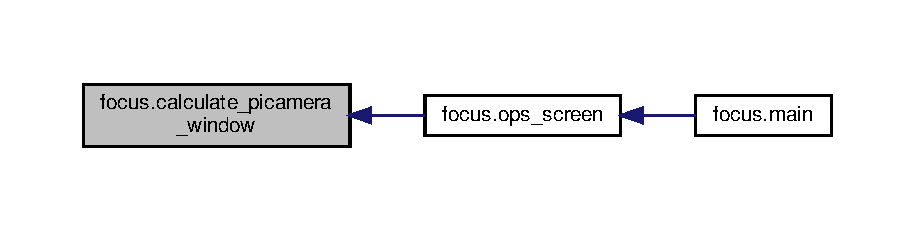
\includegraphics[width=350pt]{namespacefocus_ace593fb72d9a91bc93d3a25614a365d0_icgraph}
\end{center}
\end{figure}
\mbox{\Hypertarget{namespacefocus_aa9bf3f199d1bf68a1e49ec229dcf8c38}\label{namespacefocus_aa9bf3f199d1bf68a1e49ec229dcf8c38}} 
\index{focus@{focus}!cycle\+\_\+iso@{cycle\+\_\+iso}}
\index{cycle\+\_\+iso@{cycle\+\_\+iso}!focus@{focus}}
\subsubsection{\texorpdfstring{cycle\+\_\+iso()}{cycle\_iso()}}
{\footnotesize\ttfamily def focus.\+cycle\+\_\+iso (\begin{DoxyParamCaption}{ }\end{DoxyParamCaption})}



Void function which cycles the I\+SO value for the picamera to the next valid cycle (100, 200, 400, 800) 

Here is the caller graph for this function\+:
\nopagebreak
\begin{figure}[H]
\begin{center}
\leavevmode
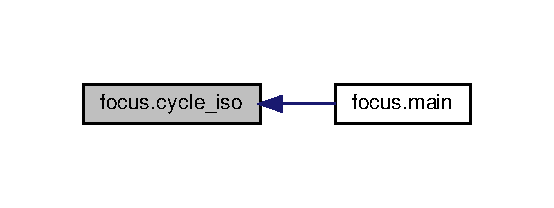
\includegraphics[width=266pt]{namespacefocus_aa9bf3f199d1bf68a1e49ec229dcf8c38_icgraph}
\end{center}
\end{figure}
\mbox{\Hypertarget{namespacefocus_a8fb78b10ef91e414ac6707d45fcd0e5b}\label{namespacefocus_a8fb78b10ef91e414ac6707d45fcd0e5b}} 
\index{focus@{focus}!decrease\+\_\+exposure@{decrease\+\_\+exposure}}
\index{decrease\+\_\+exposure@{decrease\+\_\+exposure}!focus@{focus}}
\subsubsection{\texorpdfstring{decrease\+\_\+exposure()}{decrease\_exposure()}}
{\footnotesize\ttfamily def focus.\+decrease\+\_\+exposure (\begin{DoxyParamCaption}{ }\end{DoxyParamCaption})}



Void function which decreases the exposure without letting it get all the way to 0. 

Here is the caller graph for this function\+:
\nopagebreak
\begin{figure}[H]
\begin{center}
\leavevmode
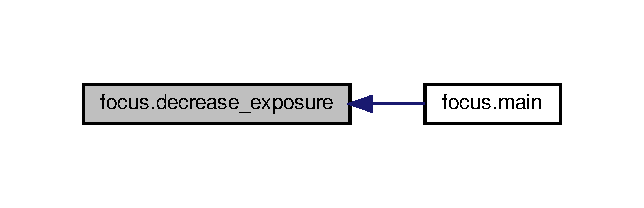
\includegraphics[width=309pt]{namespacefocus_a8fb78b10ef91e414ac6707d45fcd0e5b_icgraph}
\end{center}
\end{figure}
\mbox{\Hypertarget{namespacefocus_a7c48f36dcbc8deec93ed615925469176}\label{namespacefocus_a7c48f36dcbc8deec93ed615925469176}} 
\index{focus@{focus}!directions\+\_\+screen@{directions\+\_\+screen}}
\index{directions\+\_\+screen@{directions\+\_\+screen}!focus@{focus}}
\subsubsection{\texorpdfstring{directions\+\_\+screen()}{directions\_screen()}}
{\footnotesize\ttfamily def focus.\+directions\+\_\+screen (\begin{DoxyParamCaption}\item[{}]{screen,  }\item[{}]{font,  }\item[{}]{margin,  }\item[{}]{font\+\_\+size }\end{DoxyParamCaption})}



This is the generator for the initial directions screen. 

Prints red text on the black screen, and returns nothing. The blit changes are not activated until the pygame.\+display.\+update() is called.


\begin{DoxyParams}{Parameters}
{\em screen} & Pygame object representing the display we are operating on \\
\hline
{\em font} & Pygame object holding the font information \\
\hline
{\em margin} & int value of how far to space text lines (our margins). Additionally, this influences text position. \\
\hline
{\em font\+\_\+size} & int value for how large our font should be. Additionally, this influences text position. \\
\hline
\end{DoxyParams}
Here is the caller graph for this function\+:
\nopagebreak
\begin{figure}[H]
\begin{center}
\leavevmode
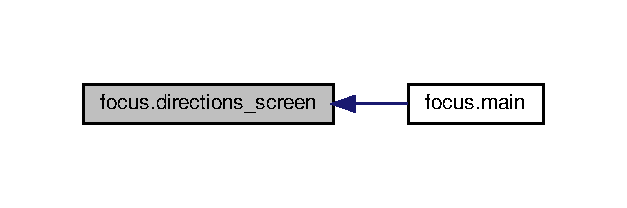
\includegraphics[width=301pt]{namespacefocus_a7c48f36dcbc8deec93ed615925469176_icgraph}
\end{center}
\end{figure}
\mbox{\Hypertarget{namespacefocus_a4dd9a598e7bc093873342c129ba80c98}\label{namespacefocus_a4dd9a598e7bc093873342c129ba80c98}} 
\index{focus@{focus}!increase\+\_\+exposure@{increase\+\_\+exposure}}
\index{increase\+\_\+exposure@{increase\+\_\+exposure}!focus@{focus}}
\subsubsection{\texorpdfstring{increase\+\_\+exposure()}{increase\_exposure()}}
{\footnotesize\ttfamily def focus.\+increase\+\_\+exposure (\begin{DoxyParamCaption}{ }\end{DoxyParamCaption})}



Void function which increases the exposure without letting it get all the way to our arbitrary M\+A\+X\+\_\+\+E\+XP. 

Here is the caller graph for this function\+:
\nopagebreak
\begin{figure}[H]
\begin{center}
\leavevmode
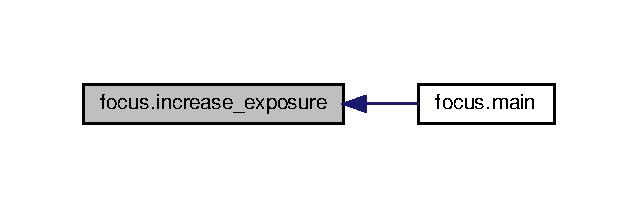
\includegraphics[width=306pt]{namespacefocus_a4dd9a598e7bc093873342c129ba80c98_icgraph}
\end{center}
\end{figure}
\mbox{\Hypertarget{namespacefocus_a813bbce9c83fa23eae05039332cf3d8a}\label{namespacefocus_a813bbce9c83fa23eae05039332cf3d8a}} 
\index{focus@{focus}!main@{main}}
\index{main@{main}!focus@{focus}}
\subsubsection{\texorpdfstring{main()}{main()}}
{\footnotesize\ttfamily def focus.\+main (\begin{DoxyParamCaption}{ }\end{DoxyParamCaption})}



This is the main execution script. 

The windows are called in order. Pygame events are used to capture keypresses from the user. These are hardcoded key bindings. Once the code is complete, or in System\+Exit conditions, cleanup methods are called for G\+P\+IO, picamera, and pygame if they were initialized previously. Here is the call graph for this function\+:
\nopagebreak
\begin{figure}[H]
\begin{center}
\leavevmode
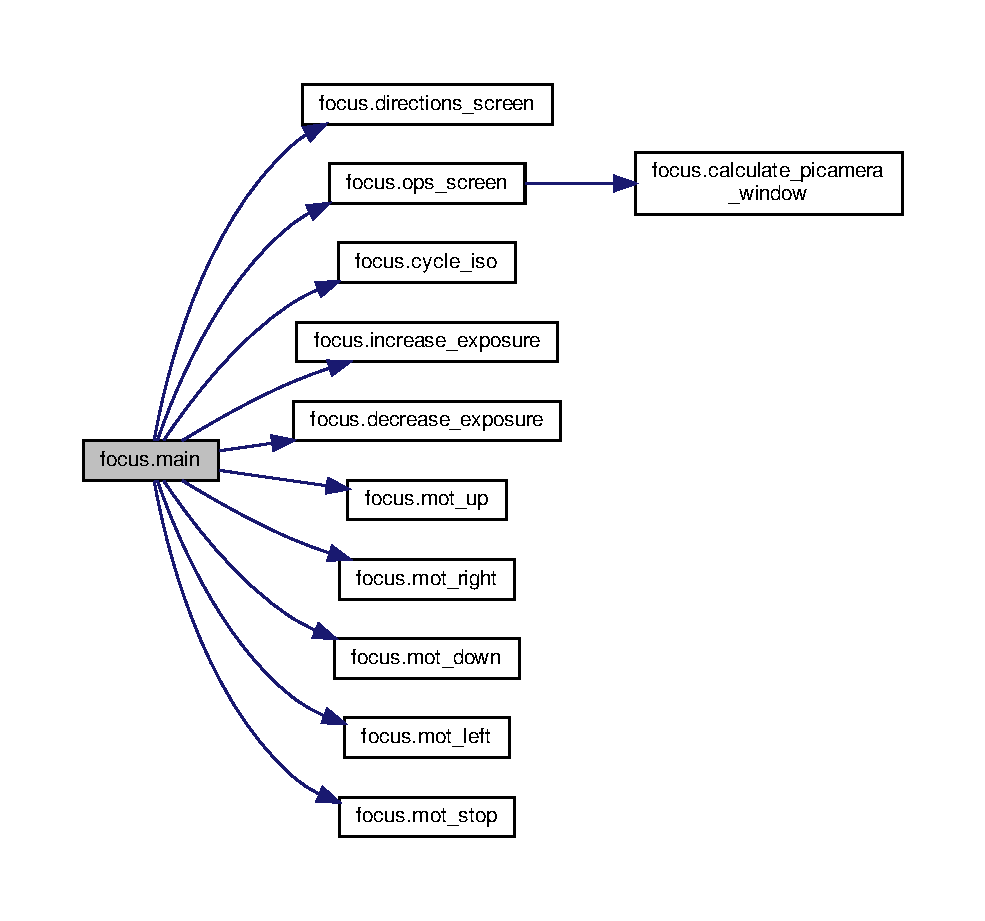
\includegraphics[width=350pt]{namespacefocus_a813bbce9c83fa23eae05039332cf3d8a_cgraph}
\end{center}
\end{figure}
\mbox{\Hypertarget{namespacefocus_ab92c9c6869b0af6ce3a5920ef8554190}\label{namespacefocus_ab92c9c6869b0af6ce3a5920ef8554190}} 
\index{focus@{focus}!mot\+\_\+down@{mot\+\_\+down}}
\index{mot\+\_\+down@{mot\+\_\+down}!focus@{focus}}
\subsubsection{\texorpdfstring{mot\+\_\+down()}{mot\_down()}}
{\footnotesize\ttfamily def focus.\+mot\+\_\+down (\begin{DoxyParamCaption}{ }\end{DoxyParamCaption})}



Void function to set the motor bits to decrease the scope\textquotesingle{}s altitude. 

Here is the caller graph for this function\+:
\nopagebreak
\begin{figure}[H]
\begin{center}
\leavevmode
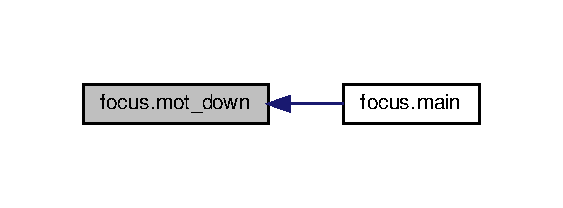
\includegraphics[width=270pt]{namespacefocus_ab92c9c6869b0af6ce3a5920ef8554190_icgraph}
\end{center}
\end{figure}
\mbox{\Hypertarget{namespacefocus_ace370021c60f38a82ce96e69a482cbe3}\label{namespacefocus_ace370021c60f38a82ce96e69a482cbe3}} 
\index{focus@{focus}!mot\+\_\+left@{mot\+\_\+left}}
\index{mot\+\_\+left@{mot\+\_\+left}!focus@{focus}}
\subsubsection{\texorpdfstring{mot\+\_\+left()}{mot\_left()}}
{\footnotesize\ttfamily def focus.\+mot\+\_\+left (\begin{DoxyParamCaption}{ }\end{DoxyParamCaption})}



Void function to set the motor bits for counter-\/clockwise azimuth adjustment. 

Here is the caller graph for this function\+:
\nopagebreak
\begin{figure}[H]
\begin{center}
\leavevmode
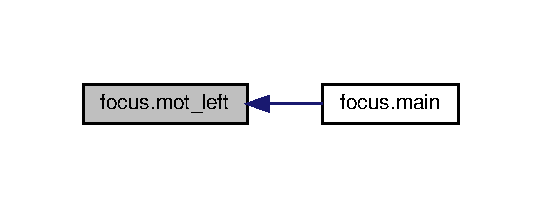
\includegraphics[width=260pt]{namespacefocus_ace370021c60f38a82ce96e69a482cbe3_icgraph}
\end{center}
\end{figure}
\mbox{\Hypertarget{namespacefocus_a9939d6f9388d8eb82625bd8e3af6f894}\label{namespacefocus_a9939d6f9388d8eb82625bd8e3af6f894}} 
\index{focus@{focus}!mot\+\_\+right@{mot\+\_\+right}}
\index{mot\+\_\+right@{mot\+\_\+right}!focus@{focus}}
\subsubsection{\texorpdfstring{mot\+\_\+right()}{mot\_right()}}
{\footnotesize\ttfamily def focus.\+mot\+\_\+right (\begin{DoxyParamCaption}{ }\end{DoxyParamCaption})}



Void function to set the motor bits for clockwise azimuth adjustment. 

Here is the caller graph for this function\+:
\nopagebreak
\begin{figure}[H]
\begin{center}
\leavevmode
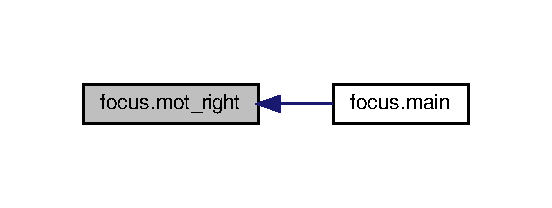
\includegraphics[width=265pt]{namespacefocus_a9939d6f9388d8eb82625bd8e3af6f894_icgraph}
\end{center}
\end{figure}
\mbox{\Hypertarget{namespacefocus_a19641d526d4c19ab6b10fc8ca9e8fe86}\label{namespacefocus_a19641d526d4c19ab6b10fc8ca9e8fe86}} 
\index{focus@{focus}!mot\+\_\+stop@{mot\+\_\+stop}}
\index{mot\+\_\+stop@{mot\+\_\+stop}!focus@{focus}}
\subsubsection{\texorpdfstring{mot\+\_\+stop()}{mot\_stop()}}
{\footnotesize\ttfamily def focus.\+mot\+\_\+stop (\begin{DoxyParamCaption}{ }\end{DoxyParamCaption})}



Void function to stop the motors. 

At high duty cycles, jumps to 10\%. At low duty cycles, the output duty cycle is decreased by 1\% each loop until reaching zero. This gradual speed reduction prevents jerky motion which may mess with the hardware. Here is the caller graph for this function\+:
\nopagebreak
\begin{figure}[H]
\begin{center}
\leavevmode
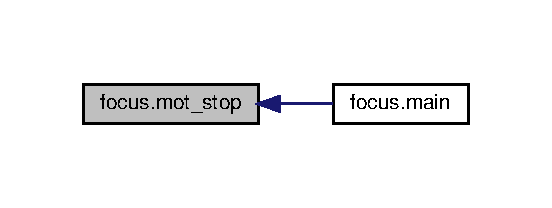
\includegraphics[width=265pt]{namespacefocus_a19641d526d4c19ab6b10fc8ca9e8fe86_icgraph}
\end{center}
\end{figure}
\mbox{\Hypertarget{namespacefocus_ad0102bfe821a43392640e33721246a8c}\label{namespacefocus_ad0102bfe821a43392640e33721246a8c}} 
\index{focus@{focus}!mot\+\_\+up@{mot\+\_\+up}}
\index{mot\+\_\+up@{mot\+\_\+up}!focus@{focus}}
\subsubsection{\texorpdfstring{mot\+\_\+up()}{mot\_up()}}
{\footnotesize\ttfamily def focus.\+mot\+\_\+up (\begin{DoxyParamCaption}{ }\end{DoxyParamCaption})}



Void function to set the motor bits to increase the scope\textquotesingle{}s altitude. 

Here is the caller graph for this function\+:
\nopagebreak
\begin{figure}[H]
\begin{center}
\leavevmode
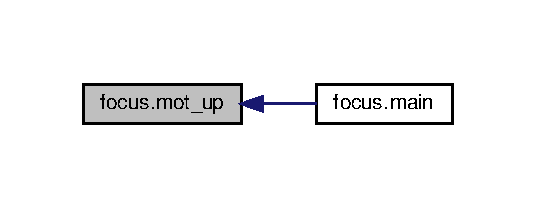
\includegraphics[width=257pt]{namespacefocus_ad0102bfe821a43392640e33721246a8c_icgraph}
\end{center}
\end{figure}
\mbox{\Hypertarget{namespacefocus_a30f8dfb1f7d958ee49491a2e359ea3e2}\label{namespacefocus_a30f8dfb1f7d958ee49491a2e359ea3e2}} 
\index{focus@{focus}!ops\+\_\+screen@{ops\+\_\+screen}}
\index{ops\+\_\+screen@{ops\+\_\+screen}!focus@{focus}}
\subsubsection{\texorpdfstring{ops\+\_\+screen()}{ops\_screen()}}
{\footnotesize\ttfamily def focus.\+ops\+\_\+screen (\begin{DoxyParamCaption}\item[{}]{screen,  }\item[{}]{font,  }\item[{}]{font\+\_\+size }\end{DoxyParamCaption})}



This is the generator for the operating window. 

Prints red text at the tippy top of the screen, and makes a red rectangle slightly larger than the expected preview window size. Also calls the camera to start the preview window. The blit changes are not activated until the pygame.\+display.\+update() is called.


\begin{DoxyParams}{Parameters}
{\em screen} & Pygame object representing the display we are operating on \\
\hline
{\em font} & Pygame object holding the font information \\
\hline
{\em font\+\_\+size} & int value for how large our font should be. In this screen, it is used to add margins to the red rectangle. \\
\hline
\end{DoxyParams}
Here is the call graph for this function\+:
\nopagebreak
\begin{figure}[H]
\begin{center}
\leavevmode
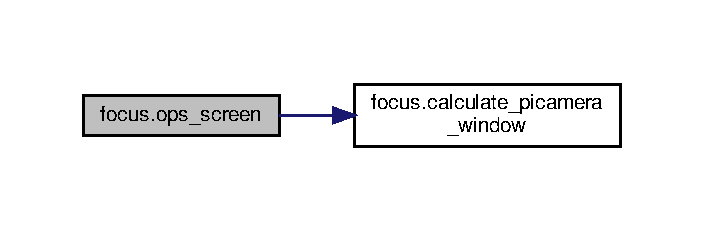
\includegraphics[width=338pt]{namespacefocus_a30f8dfb1f7d958ee49491a2e359ea3e2_cgraph}
\end{center}
\end{figure}
Here is the caller graph for this function\+:
\nopagebreak
\begin{figure}[H]
\begin{center}
\leavevmode
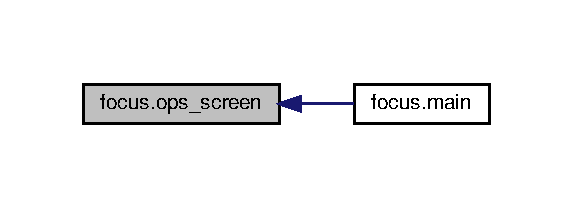
\includegraphics[width=275pt]{namespacefocus_a30f8dfb1f7d958ee49491a2e359ea3e2_icgraph}
\end{center}
\end{figure}


\subsection{Variable Documentation}
\mbox{\Hypertarget{namespacefocus_a4b9a0e4629814a6b99bd65e3200fe3bd}\label{namespacefocus_a4b9a0e4629814a6b99bd65e3200fe3bd}} 
\index{focus@{focus}!A\+P\+I\+N1@{A\+P\+I\+N1}}
\index{A\+P\+I\+N1@{A\+P\+I\+N1}!focus@{focus}}
\subsubsection{\texorpdfstring{A\+P\+I\+N1}{APIN1}}
{\footnotesize\ttfamily int focus.\+A\+P\+I\+N1 = 27}

\mbox{\Hypertarget{namespacefocus_aa7f17fd9c88f9bc5cf789df5cc73a20a}\label{namespacefocus_aa7f17fd9c88f9bc5cf789df5cc73a20a}} 
\index{focus@{focus}!A\+P\+I\+N2@{A\+P\+I\+N2}}
\index{A\+P\+I\+N2@{A\+P\+I\+N2}!focus@{focus}}
\subsubsection{\texorpdfstring{A\+P\+I\+N2}{APIN2}}
{\footnotesize\ttfamily int focus.\+A\+P\+I\+N2 = 22}

\mbox{\Hypertarget{namespacefocus_a358eaeffe0790a67619dfd820f2d66b5}\label{namespacefocus_a358eaeffe0790a67619dfd820f2d66b5}} 
\index{focus@{focus}!A\+P\+I\+NP@{A\+P\+I\+NP}}
\index{A\+P\+I\+NP@{A\+P\+I\+NP}!focus@{focus}}
\subsubsection{\texorpdfstring{A\+P\+I\+NP}{APINP}}
{\footnotesize\ttfamily int focus.\+A\+P\+I\+NP = 17}

\mbox{\Hypertarget{namespacefocus_a87a409792b8a912c225495a99b855b51}\label{namespacefocus_a87a409792b8a912c225495a99b855b51}} 
\index{focus@{focus}!B\+L\+A\+CK@{B\+L\+A\+CK}}
\index{B\+L\+A\+CK@{B\+L\+A\+CK}!focus@{focus}}
\subsubsection{\texorpdfstring{B\+L\+A\+CK}{BLACK}}
{\footnotesize\ttfamily tuple focus.\+B\+L\+A\+CK = (0, 0, 0)}

\mbox{\Hypertarget{namespacefocus_a9234861385a237ef6a50b00f5ab54f1c}\label{namespacefocus_a9234861385a237ef6a50b00f5ab54f1c}} 
\index{focus@{focus}!B\+P\+I\+N1@{B\+P\+I\+N1}}
\index{B\+P\+I\+N1@{B\+P\+I\+N1}!focus@{focus}}
\subsubsection{\texorpdfstring{B\+P\+I\+N1}{BPIN1}}
{\footnotesize\ttfamily int focus.\+B\+P\+I\+N1 = 10}

\mbox{\Hypertarget{namespacefocus_ae83fcc832e2b5c6a0281655870eae658}\label{namespacefocus_ae83fcc832e2b5c6a0281655870eae658}} 
\index{focus@{focus}!B\+P\+I\+N2@{B\+P\+I\+N2}}
\index{B\+P\+I\+N2@{B\+P\+I\+N2}!focus@{focus}}
\subsubsection{\texorpdfstring{B\+P\+I\+N2}{BPIN2}}
{\footnotesize\ttfamily int focus.\+B\+P\+I\+N2 = 9}

\mbox{\Hypertarget{namespacefocus_a88336729338c9d4ef54e14f02f406c1b}\label{namespacefocus_a88336729338c9d4ef54e14f02f406c1b}} 
\index{focus@{focus}!B\+P\+I\+NP@{B\+P\+I\+NP}}
\index{B\+P\+I\+NP@{B\+P\+I\+NP}!focus@{focus}}
\subsubsection{\texorpdfstring{B\+P\+I\+NP}{BPINP}}
{\footnotesize\ttfamily int focus.\+B\+P\+I\+NP = 11}

\mbox{\Hypertarget{namespacefocus_a2c64f595bbe297e961b55c735e7023c5}\label{namespacefocus_a2c64f595bbe297e961b55c735e7023c5}} 
\index{focus@{focus}!C\+AM@{C\+AM}}
\index{C\+AM@{C\+AM}!focus@{focus}}
\subsubsection{\texorpdfstring{C\+AM}{CAM}}
{\footnotesize\ttfamily focus.\+C\+AM = picamera.\+Pi\+Camera()}

\mbox{\Hypertarget{namespacefocus_a577e326aeb1867de857503429538fca3}\label{namespacefocus_a577e326aeb1867de857503429538fca3}} 
\index{focus@{focus}!C\+U\+R\+R\+\_\+H@{C\+U\+R\+R\+\_\+H}}
\index{C\+U\+R\+R\+\_\+H@{C\+U\+R\+R\+\_\+H}!focus@{focus}}
\subsubsection{\texorpdfstring{C\+U\+R\+R\+\_\+H}{CURR\_H}}
{\footnotesize\ttfamily focus.\+C\+U\+R\+R\+\_\+H = P\+Y\+G\+\_\+\+I\+N\+F.\+current\+\_\+h}

\mbox{\Hypertarget{namespacefocus_a2cf00646d7ebef8c88685295c224630e}\label{namespacefocus_a2cf00646d7ebef8c88685295c224630e}} 
\index{focus@{focus}!C\+U\+R\+R\+\_\+W@{C\+U\+R\+R\+\_\+W}}
\index{C\+U\+R\+R\+\_\+W@{C\+U\+R\+R\+\_\+W}!focus@{focus}}
\subsubsection{\texorpdfstring{C\+U\+R\+R\+\_\+W}{CURR\_W}}
{\footnotesize\ttfamily focus.\+C\+U\+R\+R\+\_\+W = P\+Y\+G\+\_\+\+I\+N\+F.\+current\+\_\+w}

\mbox{\Hypertarget{namespacefocus_aea3f9d81f82a645ab78f964477e8f30a}\label{namespacefocus_aea3f9d81f82a645ab78f964477e8f30a}} 
\index{focus@{focus}!D\+CA@{D\+CA}}
\index{D\+CA@{D\+CA}!focus@{focus}}
\subsubsection{\texorpdfstring{D\+CA}{DCA}}
{\footnotesize\ttfamily int focus.\+D\+CA = 0}

\mbox{\Hypertarget{namespacefocus_a7f3ad02c7918179b1964892572df8fc9}\label{namespacefocus_a7f3ad02c7918179b1964892572df8fc9}} 
\index{focus@{focus}!D\+CB@{D\+CB}}
\index{D\+CB@{D\+CB}!focus@{focus}}
\subsubsection{\texorpdfstring{D\+CB}{DCB}}
{\footnotesize\ttfamily int focus.\+D\+CB = 0}

\mbox{\Hypertarget{namespacefocus_a95643fc1eae4f9b190d9e91d48185206}\label{namespacefocus_a95643fc1eae4f9b190d9e91d48185206}} 
\index{focus@{focus}!D\+E\+B\+UG@{D\+E\+B\+UG}}
\index{D\+E\+B\+UG@{D\+E\+B\+UG}!focus@{focus}}
\subsubsection{\texorpdfstring{D\+E\+B\+UG}{DEBUG}}
{\footnotesize\ttfamily bool focus.\+D\+E\+B\+UG = True}

\mbox{\Hypertarget{namespacefocus_af9cd2a2921f660052cb32a72a681c63e}\label{namespacefocus_af9cd2a2921f660052cb32a72a681c63e}} 
\index{focus@{focus}!D\+I\+F\+F\+\_\+\+E\+XP@{D\+I\+F\+F\+\_\+\+E\+XP}}
\index{D\+I\+F\+F\+\_\+\+E\+XP@{D\+I\+F\+F\+\_\+\+E\+XP}!focus@{focus}}
\subsubsection{\texorpdfstring{D\+I\+F\+F\+\_\+\+E\+XP}{DIFF\_EXP}}
{\footnotesize\ttfamily int focus.\+D\+I\+F\+F\+\_\+\+E\+XP = 1000}

\mbox{\Hypertarget{namespacefocus_a40e81481d1b661338eda552bc7dc5513}\label{namespacefocus_a40e81481d1b661338eda552bc7dc5513}} 
\index{focus@{focus}!E\+XP@{E\+XP}}
\index{E\+XP@{E\+XP}!focus@{focus}}
\subsubsection{\texorpdfstring{E\+XP}{EXP}}
{\footnotesize\ttfamily int focus.\+E\+XP = 10000}

\mbox{\Hypertarget{namespacefocus_a9f8a2660e7de2a492738e587878c2b7a}\label{namespacefocus_a9f8a2660e7de2a492738e587878c2b7a}} 
\index{focus@{focus}!F\+R\+EQ@{F\+R\+EQ}}
\index{F\+R\+EQ@{F\+R\+EQ}!focus@{focus}}
\subsubsection{\texorpdfstring{F\+R\+EQ}{FREQ}}
{\footnotesize\ttfamily int focus.\+F\+R\+EQ = 10000}

\mbox{\Hypertarget{namespacefocus_ac7e622de99a123967bedbb1f5927ac40}\label{namespacefocus_ac7e622de99a123967bedbb1f5927ac40}} 
\index{focus@{focus}!I\+SO@{I\+SO}}
\index{I\+SO@{I\+SO}!focus@{focus}}
\subsubsection{\texorpdfstring{I\+SO}{ISO}}
{\footnotesize\ttfamily int focus.\+I\+SO = 200}

\mbox{\Hypertarget{namespacefocus_a3c4a2866356f68ceb6834b38951c16a0}\label{namespacefocus_a3c4a2866356f68ceb6834b38951c16a0}} 
\index{focus@{focus}!M\+A\+X\+\_\+\+E\+XP@{M\+A\+X\+\_\+\+E\+XP}}
\index{M\+A\+X\+\_\+\+E\+XP@{M\+A\+X\+\_\+\+E\+XP}!focus@{focus}}
\subsubsection{\texorpdfstring{M\+A\+X\+\_\+\+E\+XP}{MAX\_EXP}}
{\footnotesize\ttfamily int focus.\+M\+A\+X\+\_\+\+E\+XP = 30000}

\mbox{\Hypertarget{namespacefocus_a2418021a7b6b394da695928f0d8cd16b}\label{namespacefocus_a2418021a7b6b394da695928f0d8cd16b}} 
\index{focus@{focus}!P\+W\+MA@{P\+W\+MA}}
\index{P\+W\+MA@{P\+W\+MA}!focus@{focus}}
\subsubsection{\texorpdfstring{P\+W\+MA}{PWMA}}
{\footnotesize\ttfamily focus.\+P\+W\+MA = G\+P\+I\+O.\+P\+WM(\hyperlink{namespacefocus_a358eaeffe0790a67619dfd820f2d66b5}{A\+P\+I\+NP}, \hyperlink{namespacefocus_a9f8a2660e7de2a492738e587878c2b7a}{F\+R\+EQ})}

\mbox{\Hypertarget{namespacefocus_a9e16a63e33dd8dd160996df16dacb633}\label{namespacefocus_a9e16a63e33dd8dd160996df16dacb633}} 
\index{focus@{focus}!P\+W\+MB@{P\+W\+MB}}
\index{P\+W\+MB@{P\+W\+MB}!focus@{focus}}
\subsubsection{\texorpdfstring{P\+W\+MB}{PWMB}}
{\footnotesize\ttfamily focus.\+P\+W\+MB = G\+P\+I\+O.\+P\+WM(\hyperlink{namespacefocus_a88336729338c9d4ef54e14f02f406c1b}{B\+P\+I\+NP}, \hyperlink{namespacefocus_a9f8a2660e7de2a492738e587878c2b7a}{F\+R\+EQ})}

\mbox{\Hypertarget{namespacefocus_acc5e8b5ab47d18ad8776c429e3a3a4b7}\label{namespacefocus_acc5e8b5ab47d18ad8776c429e3a3a4b7}} 
\index{focus@{focus}!R\+ED@{R\+ED}}
\index{R\+ED@{R\+ED}!focus@{focus}}
\subsubsection{\texorpdfstring{R\+ED}{RED}}
{\footnotesize\ttfamily tuple focus.\+R\+ED = (255, 0, 0)}


\chapter{Class Documentation}
\hypertarget{classgtk__class}{}\section{gtk\+\_\+class Class Reference}
\label{classgtk__class}\index{gtk\+\_\+class@{gtk\+\_\+class}}


{\ttfamily \#include $<$gtk\+\_\+\+Lun\+Aero.\+hpp$>$}



Collaboration diagram for gtk\+\_\+class\+:
\nopagebreak
\begin{figure}[H]
\begin{center}
\leavevmode
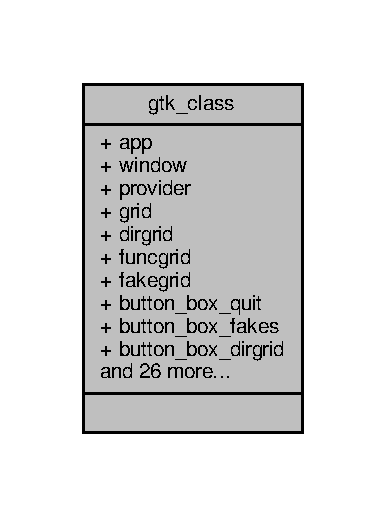
\includegraphics[width=185pt]{classgtk__class__coll__graph}
\end{center}
\end{figure}
\subsection*{Static Public Attributes}
\begin{DoxyCompactItemize}
\item 
static Gtk\+Application $\ast$ \hyperlink{classgtk__class_ae45e5712c6b5c5f0fa42a60aaff9f936}{app}
\item 
static Gtk\+Widget $\ast$ \hyperlink{classgtk__class_aa3947dc5d9f91482508977971c1a7ca2}{window}
\item 
static Gtk\+Css\+Provider $\ast$ \hyperlink{classgtk__class_a51f72983ecaccf83bb79d3d441754951}{provider}
\item 
static Gtk\+Widget $\ast$ \hyperlink{classgtk__class_aba5ba60ac9d62d3821667c89d12511fc}{grid}
\item 
static Gtk\+Widget $\ast$ \hyperlink{classgtk__class_a7fc243eec0ab61cdd6021c5f635dd40b}{dirgrid}
\item 
static Gtk\+Widget $\ast$ \hyperlink{classgtk__class_abd69dffa09078b21b628725bf1733682}{funcgrid}
\item 
static Gtk\+Widget $\ast$ \hyperlink{classgtk__class_a44907d6d72a937b0c3b6ab571e13533a}{fakegrid}
\item 
static Gtk\+Widget $\ast$ \hyperlink{classgtk__class_a291f7b187718826e0da79375375fe03f}{button\+\_\+box\+\_\+quit}
\item 
static Gtk\+Widget $\ast$ \hyperlink{classgtk__class_a4816355ec87898c40b8a3a450c7a0a75}{button\+\_\+box\+\_\+fakes}
\item 
static Gtk\+Widget $\ast$ \hyperlink{classgtk__class_aa310a332eba52f28d8819f1d419c3ca7}{button\+\_\+box\+\_\+dirgrid}
\item 
static Gtk\+Widget $\ast$ \hyperlink{classgtk__class_ab3c5243bcab4bc09a167737dd86c9cde}{button\+\_\+box\+\_\+redeploy}
\item 
static Gtk\+Widget $\ast$ \hyperlink{classgtk__class_a7bf2f4eb78eacf4c63f8eb5b59576e20}{button\+\_\+box\+\_\+funcs}
\item 
static Gtk\+Widget $\ast$ \hyperlink{classgtk__class_a0234a576c91f5d8999260eac4b6968b7}{button\+\_\+box\+\_\+activate}
\item 
static Gtk\+Widget $\ast$ \hyperlink{classgtk__class_aa6d7ef2e235a1b86782298fba1e191fa}{exit\+\_\+button}
\item 
static Gtk\+Widget $\ast$ \hyperlink{classgtk__class_aabb26f9d552a0a7e1177ec74feb838ff}{button\+\_\+up}
\item 
static Gtk\+Widget $\ast$ \hyperlink{classgtk__class_a709b242e98b6984e63a3469b2b420825}{button\+\_\+down}
\item 
static Gtk\+Widget $\ast$ \hyperlink{classgtk__class_a85b7fc192640e55afb364b3aaba0b0da}{button\+\_\+left}
\item 
static Gtk\+Widget $\ast$ \hyperlink{classgtk__class_a56405f6c6e75af4663741acc1432283c}{button\+\_\+right}
\item 
static Gtk\+Widget $\ast$ \hyperlink{classgtk__class_abf3f76bf2b007424210c597d954e7128}{button\+\_\+stop}
\item 
static Gtk\+Widget $\ast$ \hyperlink{classgtk__class_a3cb8e7ae140ae9c1b251f47aa70b570a}{button\+\_\+camera\+\_\+command}
\item 
static Gtk\+Widget $\ast$ \hyperlink{classgtk__class_ac9244ecad7ca4980e6744d333d623531}{button\+\_\+shutter\+\_\+up}
\item 
static Gtk\+Widget $\ast$ \hyperlink{classgtk__class_a5a16623a8e86c902492da7a2623ba7ed}{button\+\_\+shutter\+\_\+down}
\item 
static Gtk\+Widget $\ast$ \hyperlink{classgtk__class_ae7baa3e70983464d83caad8045f84111}{button\+\_\+shutter\+\_\+up\+\_\+up}
\item 
static Gtk\+Widget $\ast$ \hyperlink{classgtk__class_aa65822395ff08ca84df030062ff89c7f}{button\+\_\+shutter\+\_\+down\+\_\+down}
\item 
static Gtk\+Widget $\ast$ \hyperlink{classgtk__class_a2c851f4a856bc05adbeafa3ea9e9d321}{button\+\_\+iso}
\item 
static Gtk\+Widget $\ast$ \hyperlink{classgtk__class_a3b4676bf0e1502cf55fa859a338370ba}{button\+\_\+record}
\item 
static Gtk\+Widget $\ast$ \hyperlink{classgtk__class_a573da740beee14061237c96c9ede3cce}{text\+\_\+status}
\item 
static Gtk\+Widget $\ast$ \hyperlink{classgtk__class_a4150b41f2082f6827ba92cc14068e518}{text\+\_\+shutter}
\item 
static Gtk\+Widget $\ast$ \hyperlink{classgtk__class_a47995d83c3d5a3d2161361d5535c01ac}{text\+\_\+description}
\item 
static Gtk\+Widget $\ast$ \hyperlink{classgtk__class_a789555757e3a97cbf2208f9809737ba4}{fakebutton}
\item 
static Gtk\+Widget $\ast$ \hyperlink{classgtk__class_a8216a6db2ab7846b766bf1d6b476c968}{fakebutton2}
\item 
static Gtk\+Widget $\ast$ \hyperlink{classgtk__class_ad93a15c3ca9c2a605405ca967b99d8d3}{fakebutton3}
\item 
static Gtk\+Widget $\ast$ \hyperlink{classgtk__class_aad855c1e236264394ed7a353fc06fac5}{fakebutton4}
\item 
static Gtk\+Widget $\ast$ \hyperlink{classgtk__class_a39e7f05de43cf5c68285267198631336}{fakebutton5}
\item 
static const std\+::string \hyperlink{classgtk__class_a5cb715b2c56782b35912923c022cb08e}{css\+\_\+string} = \hyperlink{gtk__LunAero_8hpp_adb72df5ed4fc630244a078d8d8634b1d}{get\+\_\+css\+\_\+string}()
\item 
static gulong \hyperlink{classgtk__class_a7599d9e82fd4e3a6215730f96719d7cc}{key\+\_\+id}
\end{DoxyCompactItemize}


\subsection{Detailed Description}
This is a class to hold the various G\+TK widgets and whatnots. 

\subsection{Member Data Documentation}
\mbox{\Hypertarget{classgtk__class_ae45e5712c6b5c5f0fa42a60aaff9f936}\label{classgtk__class_ae45e5712c6b5c5f0fa42a60aaff9f936}} 
\index{gtk\+\_\+class@{gtk\+\_\+class}!app@{app}}
\index{app@{app}!gtk\+\_\+class@{gtk\+\_\+class}}
\subsubsection{\texorpdfstring{app}{app}}
{\footnotesize\ttfamily Gtk\+Application$\ast$ gtk\+\_\+class\+::app\hspace{0.3cm}{\ttfamily [inline]}, {\ttfamily [static]}}

G\+TK Main Application \mbox{\Hypertarget{classgtk__class_a0234a576c91f5d8999260eac4b6968b7}\label{classgtk__class_a0234a576c91f5d8999260eac4b6968b7}} 
\index{gtk\+\_\+class@{gtk\+\_\+class}!button\+\_\+box\+\_\+activate@{button\+\_\+box\+\_\+activate}}
\index{button\+\_\+box\+\_\+activate@{button\+\_\+box\+\_\+activate}!gtk\+\_\+class@{gtk\+\_\+class}}
\subsubsection{\texorpdfstring{button\+\_\+box\+\_\+activate}{button\_box\_activate}}
{\footnotesize\ttfamily Gtk\+Widget$\ast$ gtk\+\_\+class\+::button\+\_\+box\+\_\+activate\hspace{0.3cm}{\ttfamily [inline]}, {\ttfamily [static]}}

Container for the \char`\"{}start recording\char`\"{} button \mbox{\Hypertarget{classgtk__class_aa310a332eba52f28d8819f1d419c3ca7}\label{classgtk__class_aa310a332eba52f28d8819f1d419c3ca7}} 
\index{gtk\+\_\+class@{gtk\+\_\+class}!button\+\_\+box\+\_\+dirgrid@{button\+\_\+box\+\_\+dirgrid}}
\index{button\+\_\+box\+\_\+dirgrid@{button\+\_\+box\+\_\+dirgrid}!gtk\+\_\+class@{gtk\+\_\+class}}
\subsubsection{\texorpdfstring{button\+\_\+box\+\_\+dirgrid}{button\_box\_dirgrid}}
{\footnotesize\ttfamily Gtk\+Widget$\ast$ gtk\+\_\+class\+::button\+\_\+box\+\_\+dirgrid\hspace{0.3cm}{\ttfamily [inline]}, {\ttfamily [static]}}

Container for all of the directional pad buttons \mbox{\Hypertarget{classgtk__class_a4816355ec87898c40b8a3a450c7a0a75}\label{classgtk__class_a4816355ec87898c40b8a3a450c7a0a75}} 
\index{gtk\+\_\+class@{gtk\+\_\+class}!button\+\_\+box\+\_\+fakes@{button\+\_\+box\+\_\+fakes}}
\index{button\+\_\+box\+\_\+fakes@{button\+\_\+box\+\_\+fakes}!gtk\+\_\+class@{gtk\+\_\+class}}
\subsubsection{\texorpdfstring{button\+\_\+box\+\_\+fakes}{button\_box\_fakes}}
{\footnotesize\ttfamily Gtk\+Widget$\ast$ gtk\+\_\+class\+::button\+\_\+box\+\_\+fakes\hspace{0.3cm}{\ttfamily [inline]}, {\ttfamily [static]}}

Container for all of the fake buttons \mbox{\Hypertarget{classgtk__class_a7bf2f4eb78eacf4c63f8eb5b59576e20}\label{classgtk__class_a7bf2f4eb78eacf4c63f8eb5b59576e20}} 
\index{gtk\+\_\+class@{gtk\+\_\+class}!button\+\_\+box\+\_\+funcs@{button\+\_\+box\+\_\+funcs}}
\index{button\+\_\+box\+\_\+funcs@{button\+\_\+box\+\_\+funcs}!gtk\+\_\+class@{gtk\+\_\+class}}
\subsubsection{\texorpdfstring{button\+\_\+box\+\_\+funcs}{button\_box\_funcs}}
{\footnotesize\ttfamily Gtk\+Widget$\ast$ gtk\+\_\+class\+::button\+\_\+box\+\_\+funcs\hspace{0.3cm}{\ttfamily [inline]}, {\ttfamily [static]}}

Container for all of the I\+S\+O/\+Shutter editing buttons \mbox{\Hypertarget{classgtk__class_a291f7b187718826e0da79375375fe03f}\label{classgtk__class_a291f7b187718826e0da79375375fe03f}} 
\index{gtk\+\_\+class@{gtk\+\_\+class}!button\+\_\+box\+\_\+quit@{button\+\_\+box\+\_\+quit}}
\index{button\+\_\+box\+\_\+quit@{button\+\_\+box\+\_\+quit}!gtk\+\_\+class@{gtk\+\_\+class}}
\subsubsection{\texorpdfstring{button\+\_\+box\+\_\+quit}{button\_box\_quit}}
{\footnotesize\ttfamily Gtk\+Widget$\ast$ gtk\+\_\+class\+::button\+\_\+box\+\_\+quit\hspace{0.3cm}{\ttfamily [inline]}, {\ttfamily [static]}}

Quit button container \mbox{\Hypertarget{classgtk__class_ab3c5243bcab4bc09a167737dd86c9cde}\label{classgtk__class_ab3c5243bcab4bc09a167737dd86c9cde}} 
\index{gtk\+\_\+class@{gtk\+\_\+class}!button\+\_\+box\+\_\+redeploy@{button\+\_\+box\+\_\+redeploy}}
\index{button\+\_\+box\+\_\+redeploy@{button\+\_\+box\+\_\+redeploy}!gtk\+\_\+class@{gtk\+\_\+class}}
\subsubsection{\texorpdfstring{button\+\_\+box\+\_\+redeploy}{button\_box\_redeploy}}
{\footnotesize\ttfamily Gtk\+Widget$\ast$ gtk\+\_\+class\+::button\+\_\+box\+\_\+redeploy\hspace{0.3cm}{\ttfamily [inline]}, {\ttfamily [static]}}

Container for the camera refresh button \mbox{\Hypertarget{classgtk__class_a3cb8e7ae140ae9c1b251f47aa70b570a}\label{classgtk__class_a3cb8e7ae140ae9c1b251f47aa70b570a}} 
\index{gtk\+\_\+class@{gtk\+\_\+class}!button\+\_\+camera\+\_\+command@{button\+\_\+camera\+\_\+command}}
\index{button\+\_\+camera\+\_\+command@{button\+\_\+camera\+\_\+command}!gtk\+\_\+class@{gtk\+\_\+class}}
\subsubsection{\texorpdfstring{button\+\_\+camera\+\_\+command}{button\_camera\_command}}
{\footnotesize\ttfamily Gtk\+Widget$\ast$ gtk\+\_\+class\+::button\+\_\+camera\+\_\+command\hspace{0.3cm}{\ttfamily [inline]}, {\ttfamily [static]}}

refresh preview camera button \mbox{\Hypertarget{classgtk__class_a709b242e98b6984e63a3469b2b420825}\label{classgtk__class_a709b242e98b6984e63a3469b2b420825}} 
\index{gtk\+\_\+class@{gtk\+\_\+class}!button\+\_\+down@{button\+\_\+down}}
\index{button\+\_\+down@{button\+\_\+down}!gtk\+\_\+class@{gtk\+\_\+class}}
\subsubsection{\texorpdfstring{button\+\_\+down}{button\_down}}
{\footnotesize\ttfamily Gtk\+Widget$\ast$ gtk\+\_\+class\+::button\+\_\+down\hspace{0.3cm}{\ttfamily [inline]}, {\ttfamily [static]}}

movement down button \mbox{\Hypertarget{classgtk__class_a2c851f4a856bc05adbeafa3ea9e9d321}\label{classgtk__class_a2c851f4a856bc05adbeafa3ea9e9d321}} 
\index{gtk\+\_\+class@{gtk\+\_\+class}!button\+\_\+iso@{button\+\_\+iso}}
\index{button\+\_\+iso@{button\+\_\+iso}!gtk\+\_\+class@{gtk\+\_\+class}}
\subsubsection{\texorpdfstring{button\+\_\+iso}{button\_iso}}
{\footnotesize\ttfamily Gtk\+Widget$\ast$ gtk\+\_\+class\+::button\+\_\+iso\hspace{0.3cm}{\ttfamily [inline]}, {\ttfamily [static]}}

cycle I\+SO button \mbox{\Hypertarget{classgtk__class_a85b7fc192640e55afb364b3aaba0b0da}\label{classgtk__class_a85b7fc192640e55afb364b3aaba0b0da}} 
\index{gtk\+\_\+class@{gtk\+\_\+class}!button\+\_\+left@{button\+\_\+left}}
\index{button\+\_\+left@{button\+\_\+left}!gtk\+\_\+class@{gtk\+\_\+class}}
\subsubsection{\texorpdfstring{button\+\_\+left}{button\_left}}
{\footnotesize\ttfamily Gtk\+Widget$\ast$ gtk\+\_\+class\+::button\+\_\+left\hspace{0.3cm}{\ttfamily [inline]}, {\ttfamily [static]}}

movement left button \mbox{\Hypertarget{classgtk__class_a3b4676bf0e1502cf55fa859a338370ba}\label{classgtk__class_a3b4676bf0e1502cf55fa859a338370ba}} 
\index{gtk\+\_\+class@{gtk\+\_\+class}!button\+\_\+record@{button\+\_\+record}}
\index{button\+\_\+record@{button\+\_\+record}!gtk\+\_\+class@{gtk\+\_\+class}}
\subsubsection{\texorpdfstring{button\+\_\+record}{button\_record}}
{\footnotesize\ttfamily Gtk\+Widget$\ast$ gtk\+\_\+class\+::button\+\_\+record\hspace{0.3cm}{\ttfamily [inline]}, {\ttfamily [static]}}

begin recording button \mbox{\Hypertarget{classgtk__class_a56405f6c6e75af4663741acc1432283c}\label{classgtk__class_a56405f6c6e75af4663741acc1432283c}} 
\index{gtk\+\_\+class@{gtk\+\_\+class}!button\+\_\+right@{button\+\_\+right}}
\index{button\+\_\+right@{button\+\_\+right}!gtk\+\_\+class@{gtk\+\_\+class}}
\subsubsection{\texorpdfstring{button\+\_\+right}{button\_right}}
{\footnotesize\ttfamily Gtk\+Widget$\ast$ gtk\+\_\+class\+::button\+\_\+right\hspace{0.3cm}{\ttfamily [inline]}, {\ttfamily [static]}}

movement right button \mbox{\Hypertarget{classgtk__class_a5a16623a8e86c902492da7a2623ba7ed}\label{classgtk__class_a5a16623a8e86c902492da7a2623ba7ed}} 
\index{gtk\+\_\+class@{gtk\+\_\+class}!button\+\_\+shutter\+\_\+down@{button\+\_\+shutter\+\_\+down}}
\index{button\+\_\+shutter\+\_\+down@{button\+\_\+shutter\+\_\+down}!gtk\+\_\+class@{gtk\+\_\+class}}
\subsubsection{\texorpdfstring{button\+\_\+shutter\+\_\+down}{button\_shutter\_down}}
{\footnotesize\ttfamily Gtk\+Widget$\ast$ gtk\+\_\+class\+::button\+\_\+shutter\+\_\+down\hspace{0.3cm}{\ttfamily [inline]}, {\ttfamily [static]}}

decrease shutter value button \mbox{\Hypertarget{classgtk__class_aa65822395ff08ca84df030062ff89c7f}\label{classgtk__class_aa65822395ff08ca84df030062ff89c7f}} 
\index{gtk\+\_\+class@{gtk\+\_\+class}!button\+\_\+shutter\+\_\+down\+\_\+down@{button\+\_\+shutter\+\_\+down\+\_\+down}}
\index{button\+\_\+shutter\+\_\+down\+\_\+down@{button\+\_\+shutter\+\_\+down\+\_\+down}!gtk\+\_\+class@{gtk\+\_\+class}}
\subsubsection{\texorpdfstring{button\+\_\+shutter\+\_\+down\+\_\+down}{button\_shutter\_down\_down}}
{\footnotesize\ttfamily Gtk\+Widget$\ast$ gtk\+\_\+class\+::button\+\_\+shutter\+\_\+down\+\_\+down\hspace{0.3cm}{\ttfamily [inline]}, {\ttfamily [static]}}

greately decrease shutter button \mbox{\Hypertarget{classgtk__class_ac9244ecad7ca4980e6744d333d623531}\label{classgtk__class_ac9244ecad7ca4980e6744d333d623531}} 
\index{gtk\+\_\+class@{gtk\+\_\+class}!button\+\_\+shutter\+\_\+up@{button\+\_\+shutter\+\_\+up}}
\index{button\+\_\+shutter\+\_\+up@{button\+\_\+shutter\+\_\+up}!gtk\+\_\+class@{gtk\+\_\+class}}
\subsubsection{\texorpdfstring{button\+\_\+shutter\+\_\+up}{button\_shutter\_up}}
{\footnotesize\ttfamily Gtk\+Widget$\ast$ gtk\+\_\+class\+::button\+\_\+shutter\+\_\+up\hspace{0.3cm}{\ttfamily [inline]}, {\ttfamily [static]}}

increase shutter value button \mbox{\Hypertarget{classgtk__class_ae7baa3e70983464d83caad8045f84111}\label{classgtk__class_ae7baa3e70983464d83caad8045f84111}} 
\index{gtk\+\_\+class@{gtk\+\_\+class}!button\+\_\+shutter\+\_\+up\+\_\+up@{button\+\_\+shutter\+\_\+up\+\_\+up}}
\index{button\+\_\+shutter\+\_\+up\+\_\+up@{button\+\_\+shutter\+\_\+up\+\_\+up}!gtk\+\_\+class@{gtk\+\_\+class}}
\subsubsection{\texorpdfstring{button\+\_\+shutter\+\_\+up\+\_\+up}{button\_shutter\_up\_up}}
{\footnotesize\ttfamily Gtk\+Widget$\ast$ gtk\+\_\+class\+::button\+\_\+shutter\+\_\+up\+\_\+up\hspace{0.3cm}{\ttfamily [inline]}, {\ttfamily [static]}}

greatly increase shutter button \mbox{\Hypertarget{classgtk__class_abf3f76bf2b007424210c597d954e7128}\label{classgtk__class_abf3f76bf2b007424210c597d954e7128}} 
\index{gtk\+\_\+class@{gtk\+\_\+class}!button\+\_\+stop@{button\+\_\+stop}}
\index{button\+\_\+stop@{button\+\_\+stop}!gtk\+\_\+class@{gtk\+\_\+class}}
\subsubsection{\texorpdfstring{button\+\_\+stop}{button\_stop}}
{\footnotesize\ttfamily Gtk\+Widget$\ast$ gtk\+\_\+class\+::button\+\_\+stop\hspace{0.3cm}{\ttfamily [inline]}, {\ttfamily [static]}}

movement stop button \mbox{\Hypertarget{classgtk__class_aabb26f9d552a0a7e1177ec74feb838ff}\label{classgtk__class_aabb26f9d552a0a7e1177ec74feb838ff}} 
\index{gtk\+\_\+class@{gtk\+\_\+class}!button\+\_\+up@{button\+\_\+up}}
\index{button\+\_\+up@{button\+\_\+up}!gtk\+\_\+class@{gtk\+\_\+class}}
\subsubsection{\texorpdfstring{button\+\_\+up}{button\_up}}
{\footnotesize\ttfamily Gtk\+Widget$\ast$ gtk\+\_\+class\+::button\+\_\+up\hspace{0.3cm}{\ttfamily [inline]}, {\ttfamily [static]}}

movement up button \mbox{\Hypertarget{classgtk__class_a5cb715b2c56782b35912923c022cb08e}\label{classgtk__class_a5cb715b2c56782b35912923c022cb08e}} 
\index{gtk\+\_\+class@{gtk\+\_\+class}!css\+\_\+string@{css\+\_\+string}}
\index{css\+\_\+string@{css\+\_\+string}!gtk\+\_\+class@{gtk\+\_\+class}}
\subsubsection{\texorpdfstring{css\+\_\+string}{css\_string}}
{\footnotesize\ttfamily const std\+::string gtk\+\_\+class\+::css\+\_\+string = \hyperlink{gtk__LunAero_8hpp_adb72df5ed4fc630244a078d8d8634b1d}{get\+\_\+css\+\_\+string}()\hspace{0.3cm}{\ttfamily [inline]}, {\ttfamily [static]}}

Holds the C\+SS string. Not an actual widtet! \mbox{\Hypertarget{classgtk__class_a7fc243eec0ab61cdd6021c5f635dd40b}\label{classgtk__class_a7fc243eec0ab61cdd6021c5f635dd40b}} 
\index{gtk\+\_\+class@{gtk\+\_\+class}!dirgrid@{dirgrid}}
\index{dirgrid@{dirgrid}!gtk\+\_\+class@{gtk\+\_\+class}}
\subsubsection{\texorpdfstring{dirgrid}{dirgrid}}
{\footnotesize\ttfamily Gtk\+Widget$\ast$ gtk\+\_\+class\+::dirgrid\hspace{0.3cm}{\ttfamily [inline]}, {\ttfamily [static]}}

Grid to hold the directional movement pad \mbox{\Hypertarget{classgtk__class_aa6d7ef2e235a1b86782298fba1e191fa}\label{classgtk__class_aa6d7ef2e235a1b86782298fba1e191fa}} 
\index{gtk\+\_\+class@{gtk\+\_\+class}!exit\+\_\+button@{exit\+\_\+button}}
\index{exit\+\_\+button@{exit\+\_\+button}!gtk\+\_\+class@{gtk\+\_\+class}}
\subsubsection{\texorpdfstring{exit\+\_\+button}{exit\_button}}
{\footnotesize\ttfamily Gtk\+Widget$\ast$ gtk\+\_\+class\+::exit\+\_\+button\hspace{0.3cm}{\ttfamily [inline]}, {\ttfamily [static]}}

exit button \mbox{\Hypertarget{classgtk__class_a789555757e3a97cbf2208f9809737ba4}\label{classgtk__class_a789555757e3a97cbf2208f9809737ba4}} 
\index{gtk\+\_\+class@{gtk\+\_\+class}!fakebutton@{fakebutton}}
\index{fakebutton@{fakebutton}!gtk\+\_\+class@{gtk\+\_\+class}}
\subsubsection{\texorpdfstring{fakebutton}{fakebutton}}
{\footnotesize\ttfamily Gtk\+Widget$\ast$ gtk\+\_\+class\+::fakebutton\hspace{0.3cm}{\ttfamily [inline]}, {\ttfamily [static]}}

fake button -\/ does nothing \mbox{\Hypertarget{classgtk__class_a8216a6db2ab7846b766bf1d6b476c968}\label{classgtk__class_a8216a6db2ab7846b766bf1d6b476c968}} 
\index{gtk\+\_\+class@{gtk\+\_\+class}!fakebutton2@{fakebutton2}}
\index{fakebutton2@{fakebutton2}!gtk\+\_\+class@{gtk\+\_\+class}}
\subsubsection{\texorpdfstring{fakebutton2}{fakebutton2}}
{\footnotesize\ttfamily Gtk\+Widget$\ast$ gtk\+\_\+class\+::fakebutton2\hspace{0.3cm}{\ttfamily [inline]}, {\ttfamily [static]}}

fake button -\/ does nothing \mbox{\Hypertarget{classgtk__class_ad93a15c3ca9c2a605405ca967b99d8d3}\label{classgtk__class_ad93a15c3ca9c2a605405ca967b99d8d3}} 
\index{gtk\+\_\+class@{gtk\+\_\+class}!fakebutton3@{fakebutton3}}
\index{fakebutton3@{fakebutton3}!gtk\+\_\+class@{gtk\+\_\+class}}
\subsubsection{\texorpdfstring{fakebutton3}{fakebutton3}}
{\footnotesize\ttfamily Gtk\+Widget$\ast$ gtk\+\_\+class\+::fakebutton3\hspace{0.3cm}{\ttfamily [inline]}, {\ttfamily [static]}}

fake button -\/ does nothing \mbox{\Hypertarget{classgtk__class_aad855c1e236264394ed7a353fc06fac5}\label{classgtk__class_aad855c1e236264394ed7a353fc06fac5}} 
\index{gtk\+\_\+class@{gtk\+\_\+class}!fakebutton4@{fakebutton4}}
\index{fakebutton4@{fakebutton4}!gtk\+\_\+class@{gtk\+\_\+class}}
\subsubsection{\texorpdfstring{fakebutton4}{fakebutton4}}
{\footnotesize\ttfamily Gtk\+Widget$\ast$ gtk\+\_\+class\+::fakebutton4\hspace{0.3cm}{\ttfamily [inline]}, {\ttfamily [static]}}

fake button -\/ does nothing \mbox{\Hypertarget{classgtk__class_a39e7f05de43cf5c68285267198631336}\label{classgtk__class_a39e7f05de43cf5c68285267198631336}} 
\index{gtk\+\_\+class@{gtk\+\_\+class}!fakebutton5@{fakebutton5}}
\index{fakebutton5@{fakebutton5}!gtk\+\_\+class@{gtk\+\_\+class}}
\subsubsection{\texorpdfstring{fakebutton5}{fakebutton5}}
{\footnotesize\ttfamily Gtk\+Widget$\ast$ gtk\+\_\+class\+::fakebutton5\hspace{0.3cm}{\ttfamily [inline]}, {\ttfamily [static]}}

fake button -\/ does nothing \mbox{\Hypertarget{classgtk__class_a44907d6d72a937b0c3b6ab571e13533a}\label{classgtk__class_a44907d6d72a937b0c3b6ab571e13533a}} 
\index{gtk\+\_\+class@{gtk\+\_\+class}!fakegrid@{fakegrid}}
\index{fakegrid@{fakegrid}!gtk\+\_\+class@{gtk\+\_\+class}}
\subsubsection{\texorpdfstring{fakegrid}{fakegrid}}
{\footnotesize\ttfamily Gtk\+Widget$\ast$ gtk\+\_\+class\+::fakegrid\hspace{0.3cm}{\ttfamily [inline]}, {\ttfamily [static]}}

Grid to hold our fakebuttons \mbox{\Hypertarget{classgtk__class_abd69dffa09078b21b628725bf1733682}\label{classgtk__class_abd69dffa09078b21b628725bf1733682}} 
\index{gtk\+\_\+class@{gtk\+\_\+class}!funcgrid@{funcgrid}}
\index{funcgrid@{funcgrid}!gtk\+\_\+class@{gtk\+\_\+class}}
\subsubsection{\texorpdfstring{funcgrid}{funcgrid}}
{\footnotesize\ttfamily Gtk\+Widget$\ast$ gtk\+\_\+class\+::funcgrid\hspace{0.3cm}{\ttfamily [inline]}, {\ttfamily [static]}}

Grid to hold function buttons \mbox{\Hypertarget{classgtk__class_aba5ba60ac9d62d3821667c89d12511fc}\label{classgtk__class_aba5ba60ac9d62d3821667c89d12511fc}} 
\index{gtk\+\_\+class@{gtk\+\_\+class}!grid@{grid}}
\index{grid@{grid}!gtk\+\_\+class@{gtk\+\_\+class}}
\subsubsection{\texorpdfstring{grid}{grid}}
{\footnotesize\ttfamily Gtk\+Widget$\ast$ gtk\+\_\+class\+::grid\hspace{0.3cm}{\ttfamily [inline]}, {\ttfamily [static]}}

Primary grid for window layout. \mbox{\Hypertarget{classgtk__class_a7599d9e82fd4e3a6215730f96719d7cc}\label{classgtk__class_a7599d9e82fd4e3a6215730f96719d7cc}} 
\index{gtk\+\_\+class@{gtk\+\_\+class}!key\+\_\+id@{key\+\_\+id}}
\index{key\+\_\+id@{key\+\_\+id}!gtk\+\_\+class@{gtk\+\_\+class}}
\subsubsection{\texorpdfstring{key\+\_\+id}{key\_id}}
{\footnotesize\ttfamily gulong gtk\+\_\+class\+::key\+\_\+id\hspace{0.3cm}{\ttfamily [inline]}, {\ttfamily [static]}}

Holds the key\+\_\+id of a button pressed on the user\textquotesingle{}s keyboard. \mbox{\Hypertarget{classgtk__class_a51f72983ecaccf83bb79d3d441754951}\label{classgtk__class_a51f72983ecaccf83bb79d3d441754951}} 
\index{gtk\+\_\+class@{gtk\+\_\+class}!provider@{provider}}
\index{provider@{provider}!gtk\+\_\+class@{gtk\+\_\+class}}
\subsubsection{\texorpdfstring{provider}{provider}}
{\footnotesize\ttfamily Gtk\+Css\+Provider$\ast$ gtk\+\_\+class\+::provider\hspace{0.3cm}{\ttfamily [inline]}, {\ttfamily [static]}}

G\+TK C\+SS provider \mbox{\Hypertarget{classgtk__class_a47995d83c3d5a3d2161361d5535c01ac}\label{classgtk__class_a47995d83c3d5a3d2161361d5535c01ac}} 
\index{gtk\+\_\+class@{gtk\+\_\+class}!text\+\_\+description@{text\+\_\+description}}
\index{text\+\_\+description@{text\+\_\+description}!gtk\+\_\+class@{gtk\+\_\+class}}
\subsubsection{\texorpdfstring{text\+\_\+description}{text\_description}}
{\footnotesize\ttfamily Gtk\+Widget$\ast$ gtk\+\_\+class\+::text\+\_\+description\hspace{0.3cm}{\ttfamily [inline]}, {\ttfamily [static]}}

Container for some blank lines that help arrange the grid \mbox{\Hypertarget{classgtk__class_a4150b41f2082f6827ba92cc14068e518}\label{classgtk__class_a4150b41f2082f6827ba92cc14068e518}} 
\index{gtk\+\_\+class@{gtk\+\_\+class}!text\+\_\+shutter@{text\+\_\+shutter}}
\index{text\+\_\+shutter@{text\+\_\+shutter}!gtk\+\_\+class@{gtk\+\_\+class}}
\subsubsection{\texorpdfstring{text\+\_\+shutter}{text\_shutter}}
{\footnotesize\ttfamily Gtk\+Widget$\ast$ gtk\+\_\+class\+::text\+\_\+shutter\hspace{0.3cm}{\ttfamily [inline]}, {\ttfamily [static]}}

Container for shutter speed label \mbox{\Hypertarget{classgtk__class_a573da740beee14061237c96c9ede3cce}\label{classgtk__class_a573da740beee14061237c96c9ede3cce}} 
\index{gtk\+\_\+class@{gtk\+\_\+class}!text\+\_\+status@{text\+\_\+status}}
\index{text\+\_\+status@{text\+\_\+status}!gtk\+\_\+class@{gtk\+\_\+class}}
\subsubsection{\texorpdfstring{text\+\_\+status}{text\_status}}
{\footnotesize\ttfamily Gtk\+Widget$\ast$ gtk\+\_\+class\+::text\+\_\+status\hspace{0.3cm}{\ttfamily [inline]}, {\ttfamily [static]}}

Container to hold the status (I\+S\+O/\+Shutter/\+Blur and Running) \mbox{\Hypertarget{classgtk__class_aa3947dc5d9f91482508977971c1a7ca2}\label{classgtk__class_aa3947dc5d9f91482508977971c1a7ca2}} 
\index{gtk\+\_\+class@{gtk\+\_\+class}!window@{window}}
\index{window@{window}!gtk\+\_\+class@{gtk\+\_\+class}}
\subsubsection{\texorpdfstring{window}{window}}
{\footnotesize\ttfamily Gtk\+Widget$\ast$ gtk\+\_\+class\+::window\hspace{0.3cm}{\ttfamily [inline]}, {\ttfamily [static]}}

Main G\+TK window 

The documentation for this class was generated from the following file\+:\begin{DoxyCompactItemize}
\item 
\hyperlink{gtk__LunAero_8hpp}{gtk\+\_\+\+Lun\+Aero.\+hpp}\end{DoxyCompactItemize}

\hypertarget{structval__addresses}{}\section{val\+\_\+addresses Struct Reference}
\label{structval__addresses}\index{val\+\_\+addresses@{val\+\_\+addresses}}


{\ttfamily \#include $<$Lun\+Aero.\+hpp$>$}



Collaboration diagram for val\+\_\+addresses\+:
\nopagebreak
\begin{figure}[H]
\begin{center}
\leavevmode
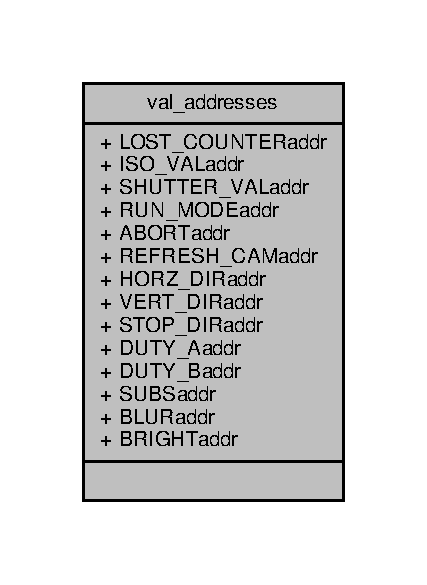
\includegraphics[width=205pt]{structval__addresses__coll__graph}
\end{center}
\end{figure}
\subsection*{Public Attributes}
\begin{DoxyCompactItemize}
\item 
volatile int $\ast$ \hyperlink{structval__addresses_a0eb119cb562c1ab4a3d68e513d439fcd}{L\+O\+S\+T\+\_\+\+C\+O\+U\+N\+T\+E\+Raddr}
\item 
volatile int $\ast$ \hyperlink{structval__addresses_a5a5f6d9a976602675639458fa735c845}{I\+S\+O\+\_\+\+V\+A\+Laddr}
\item 
volatile int $\ast$ \hyperlink{structval__addresses_a57ee2cd54ae492b38aae06975b64b0e2}{S\+H\+U\+T\+T\+E\+R\+\_\+\+V\+A\+Laddr}
\item 
volatile int $\ast$ \hyperlink{structval__addresses_aae5779146fa4fb188bb9572c20d5da4a}{R\+U\+N\+\_\+\+M\+O\+D\+Eaddr}
\item 
volatile int $\ast$ \hyperlink{structval__addresses_a0fe118a58a06a6f24181c13f97962e26}{A\+B\+O\+R\+Taddr}
\item 
volatile int $\ast$ \hyperlink{structval__addresses_a9da32da59ec29598d672ad09003491fd}{R\+E\+F\+R\+E\+S\+H\+\_\+\+C\+A\+Maddr}
\item 
volatile int $\ast$ \hyperlink{structval__addresses_aaa663924337345adb7b14897d1e7d1a5}{H\+O\+R\+Z\+\_\+\+D\+I\+Raddr}
\item 
volatile int $\ast$ \hyperlink{structval__addresses_a0bc3ea6915b32a17b4c333b865c81ea9}{V\+E\+R\+T\+\_\+\+D\+I\+Raddr}
\item 
volatile int $\ast$ \hyperlink{structval__addresses_ae9ae522d433f333dbb15a1ed5ebe70e6}{S\+T\+O\+P\+\_\+\+D\+I\+Raddr}
\item 
volatile int $\ast$ \hyperlink{structval__addresses_aadc43e056f0b10d3c772bd0ed45ae5bc}{D\+U\+T\+Y\+\_\+\+Aaddr}
\item 
volatile int $\ast$ \hyperlink{structval__addresses_a3bb48724a49aba39d68249e4714f731c}{D\+U\+T\+Y\+\_\+\+Baddr}
\item 
volatile int $\ast$ \hyperlink{structval__addresses_a2dc7beaca139f55cee0def0170611e03}{S\+U\+B\+Saddr}
\end{DoxyCompactItemize}


\subsection{Detailed Description}
Struct of addresses used across forks to store important values. Call these values with the prototype\+: $\ast$val\+\_\+ptr.E\+X\+A\+M\+P\+L\+Eaddr. These are declared inline across cpp files, requiring C++17. 

\subsection{Member Data Documentation}
\mbox{\Hypertarget{structval__addresses_a0fe118a58a06a6f24181c13f97962e26}\label{structval__addresses_a0fe118a58a06a6f24181c13f97962e26}} 
\index{val\+\_\+addresses@{val\+\_\+addresses}!A\+B\+O\+R\+Taddr@{A\+B\+O\+R\+Taddr}}
\index{A\+B\+O\+R\+Taddr@{A\+B\+O\+R\+Taddr}!val\+\_\+addresses@{val\+\_\+addresses}}
\subsubsection{\texorpdfstring{A\+B\+O\+R\+Taddr}{ABORTaddr}}
{\footnotesize\ttfamily volatile int$\ast$ val\+\_\+addresses\+::\+A\+B\+O\+R\+Taddr}

Flag to sync abort functions across code forks. If 0, run. If 1, abort. \mbox{\Hypertarget{structval__addresses_aadc43e056f0b10d3c772bd0ed45ae5bc}\label{structval__addresses_aadc43e056f0b10d3c772bd0ed45ae5bc}} 
\index{val\+\_\+addresses@{val\+\_\+addresses}!D\+U\+T\+Y\+\_\+\+Aaddr@{D\+U\+T\+Y\+\_\+\+Aaddr}}
\index{D\+U\+T\+Y\+\_\+\+Aaddr@{D\+U\+T\+Y\+\_\+\+Aaddr}!val\+\_\+addresses@{val\+\_\+addresses}}
\subsubsection{\texorpdfstring{D\+U\+T\+Y\+\_\+\+Aaddr}{DUTY\_Aaddr}}
{\footnotesize\ttfamily volatile int$\ast$ val\+\_\+addresses\+::\+D\+U\+T\+Y\+\_\+\+Aaddr}

Current duty cycle of motor A. Valid values 0-\/100. \mbox{\Hypertarget{structval__addresses_a3bb48724a49aba39d68249e4714f731c}\label{structval__addresses_a3bb48724a49aba39d68249e4714f731c}} 
\index{val\+\_\+addresses@{val\+\_\+addresses}!D\+U\+T\+Y\+\_\+\+Baddr@{D\+U\+T\+Y\+\_\+\+Baddr}}
\index{D\+U\+T\+Y\+\_\+\+Baddr@{D\+U\+T\+Y\+\_\+\+Baddr}!val\+\_\+addresses@{val\+\_\+addresses}}
\subsubsection{\texorpdfstring{D\+U\+T\+Y\+\_\+\+Baddr}{DUTY\_Baddr}}
{\footnotesize\ttfamily volatile int$\ast$ val\+\_\+addresses\+::\+D\+U\+T\+Y\+\_\+\+Baddr}

Current duty cycle of motor B. Valid values 0-\/100. \mbox{\Hypertarget{structval__addresses_aaa663924337345adb7b14897d1e7d1a5}\label{structval__addresses_aaa663924337345adb7b14897d1e7d1a5}} 
\index{val\+\_\+addresses@{val\+\_\+addresses}!H\+O\+R\+Z\+\_\+\+D\+I\+Raddr@{H\+O\+R\+Z\+\_\+\+D\+I\+Raddr}}
\index{H\+O\+R\+Z\+\_\+\+D\+I\+Raddr@{H\+O\+R\+Z\+\_\+\+D\+I\+Raddr}!val\+\_\+addresses@{val\+\_\+addresses}}
\subsubsection{\texorpdfstring{H\+O\+R\+Z\+\_\+\+D\+I\+Raddr}{HORZ\_DIRaddr}}
{\footnotesize\ttfamily volatile int$\ast$ val\+\_\+addresses\+::\+H\+O\+R\+Z\+\_\+\+D\+I\+Raddr}

Horizontal motion to be applied to motor B. Values\+: 0 = none, 1 = left, 2 = right \mbox{\Hypertarget{structval__addresses_a5a5f6d9a976602675639458fa735c845}\label{structval__addresses_a5a5f6d9a976602675639458fa735c845}} 
\index{val\+\_\+addresses@{val\+\_\+addresses}!I\+S\+O\+\_\+\+V\+A\+Laddr@{I\+S\+O\+\_\+\+V\+A\+Laddr}}
\index{I\+S\+O\+\_\+\+V\+A\+Laddr@{I\+S\+O\+\_\+\+V\+A\+Laddr}!val\+\_\+addresses@{val\+\_\+addresses}}
\subsubsection{\texorpdfstring{I\+S\+O\+\_\+\+V\+A\+Laddr}{ISO\_VALaddr}}
{\footnotesize\ttfamily volatile int$\ast$ val\+\_\+addresses\+::\+I\+S\+O\+\_\+\+V\+A\+Laddr}

Value of I\+SO selected by the user. Valid values (100, 200, 400, 800) \mbox{\Hypertarget{structval__addresses_a0eb119cb562c1ab4a3d68e513d439fcd}\label{structval__addresses_a0eb119cb562c1ab4a3d68e513d439fcd}} 
\index{val\+\_\+addresses@{val\+\_\+addresses}!L\+O\+S\+T\+\_\+\+C\+O\+U\+N\+T\+E\+Raddr@{L\+O\+S\+T\+\_\+\+C\+O\+U\+N\+T\+E\+Raddr}}
\index{L\+O\+S\+T\+\_\+\+C\+O\+U\+N\+T\+E\+Raddr@{L\+O\+S\+T\+\_\+\+C\+O\+U\+N\+T\+E\+Raddr}!val\+\_\+addresses@{val\+\_\+addresses}}
\subsubsection{\texorpdfstring{L\+O\+S\+T\+\_\+\+C\+O\+U\+N\+T\+E\+Raddr}{LOST\_COUNTERaddr}}
{\footnotesize\ttfamily volatile int$\ast$ val\+\_\+addresses\+::\+L\+O\+S\+T\+\_\+\+C\+O\+U\+N\+T\+E\+Raddr}

Counter of the number of cycles the moon has been lost. \mbox{\Hypertarget{structval__addresses_a9da32da59ec29598d672ad09003491fd}\label{structval__addresses_a9da32da59ec29598d672ad09003491fd}} 
\index{val\+\_\+addresses@{val\+\_\+addresses}!R\+E\+F\+R\+E\+S\+H\+\_\+\+C\+A\+Maddr@{R\+E\+F\+R\+E\+S\+H\+\_\+\+C\+A\+Maddr}}
\index{R\+E\+F\+R\+E\+S\+H\+\_\+\+C\+A\+Maddr@{R\+E\+F\+R\+E\+S\+H\+\_\+\+C\+A\+Maddr}!val\+\_\+addresses@{val\+\_\+addresses}}
\subsubsection{\texorpdfstring{R\+E\+F\+R\+E\+S\+H\+\_\+\+C\+A\+Maddr}{REFRESH\_CAMaddr}}
{\footnotesize\ttfamily volatile int$\ast$ val\+\_\+addresses\+::\+R\+E\+F\+R\+E\+S\+H\+\_\+\+C\+A\+Maddr}

Flag to sync camera refreshes across forks. If 0, do nothing. If 1, refresh. \mbox{\Hypertarget{structval__addresses_aae5779146fa4fb188bb9572c20d5da4a}\label{structval__addresses_aae5779146fa4fb188bb9572c20d5da4a}} 
\index{val\+\_\+addresses@{val\+\_\+addresses}!R\+U\+N\+\_\+\+M\+O\+D\+Eaddr@{R\+U\+N\+\_\+\+M\+O\+D\+Eaddr}}
\index{R\+U\+N\+\_\+\+M\+O\+D\+Eaddr@{R\+U\+N\+\_\+\+M\+O\+D\+Eaddr}!val\+\_\+addresses@{val\+\_\+addresses}}
\subsubsection{\texorpdfstring{R\+U\+N\+\_\+\+M\+O\+D\+Eaddr}{RUN\_MODEaddr}}
{\footnotesize\ttfamily volatile int$\ast$ val\+\_\+addresses\+::\+R\+U\+N\+\_\+\+M\+O\+D\+Eaddr}

Value of the current run mode. Valid values are 0 for preview/manual mode and 1 for recording/automatic mode \mbox{\Hypertarget{structval__addresses_a57ee2cd54ae492b38aae06975b64b0e2}\label{structval__addresses_a57ee2cd54ae492b38aae06975b64b0e2}} 
\index{val\+\_\+addresses@{val\+\_\+addresses}!S\+H\+U\+T\+T\+E\+R\+\_\+\+V\+A\+Laddr@{S\+H\+U\+T\+T\+E\+R\+\_\+\+V\+A\+Laddr}}
\index{S\+H\+U\+T\+T\+E\+R\+\_\+\+V\+A\+Laddr@{S\+H\+U\+T\+T\+E\+R\+\_\+\+V\+A\+Laddr}!val\+\_\+addresses@{val\+\_\+addresses}}
\subsubsection{\texorpdfstring{S\+H\+U\+T\+T\+E\+R\+\_\+\+V\+A\+Laddr}{SHUTTER\_VALaddr}}
{\footnotesize\ttfamily volatile int$\ast$ val\+\_\+addresses\+::\+S\+H\+U\+T\+T\+E\+R\+\_\+\+V\+A\+Laddr}

Value of the shutter speed selected by the user. Minimum and maximum values are determined by the hardware and limited further by code. \mbox{\Hypertarget{structval__addresses_ae9ae522d433f333dbb15a1ed5ebe70e6}\label{structval__addresses_ae9ae522d433f333dbb15a1ed5ebe70e6}} 
\index{val\+\_\+addresses@{val\+\_\+addresses}!S\+T\+O\+P\+\_\+\+D\+I\+Raddr@{S\+T\+O\+P\+\_\+\+D\+I\+Raddr}}
\index{S\+T\+O\+P\+\_\+\+D\+I\+Raddr@{S\+T\+O\+P\+\_\+\+D\+I\+Raddr}!val\+\_\+addresses@{val\+\_\+addresses}}
\subsubsection{\texorpdfstring{S\+T\+O\+P\+\_\+\+D\+I\+Raddr}{STOP\_DIRaddr}}
{\footnotesize\ttfamily volatile int$\ast$ val\+\_\+addresses\+::\+S\+T\+O\+P\+\_\+\+D\+I\+Raddr}

Stop motors selected by this flag. Values\+: 0 = none, 1 = horizontal only, 2 = vertical only, 3 = both motors. \mbox{\Hypertarget{structval__addresses_a2dc7beaca139f55cee0def0170611e03}\label{structval__addresses_a2dc7beaca139f55cee0def0170611e03}} 
\index{val\+\_\+addresses@{val\+\_\+addresses}!S\+U\+B\+Saddr@{S\+U\+B\+Saddr}}
\index{S\+U\+B\+Saddr@{S\+U\+B\+Saddr}!val\+\_\+addresses@{val\+\_\+addresses}}
\subsubsection{\texorpdfstring{S\+U\+B\+Saddr}{SUBSaddr}}
{\footnotesize\ttfamily volatile int$\ast$ val\+\_\+addresses\+::\+S\+U\+B\+Saddr}

Flag for telling the raspivid refresh algorithm if this the original run or subsequent runs being refreshed to elicit appropriate behavior. \mbox{\Hypertarget{structval__addresses_a0bc3ea6915b32a17b4c333b865c81ea9}\label{structval__addresses_a0bc3ea6915b32a17b4c333b865c81ea9}} 
\index{val\+\_\+addresses@{val\+\_\+addresses}!V\+E\+R\+T\+\_\+\+D\+I\+Raddr@{V\+E\+R\+T\+\_\+\+D\+I\+Raddr}}
\index{V\+E\+R\+T\+\_\+\+D\+I\+Raddr@{V\+E\+R\+T\+\_\+\+D\+I\+Raddr}!val\+\_\+addresses@{val\+\_\+addresses}}
\subsubsection{\texorpdfstring{V\+E\+R\+T\+\_\+\+D\+I\+Raddr}{VERT\_DIRaddr}}
{\footnotesize\ttfamily volatile int$\ast$ val\+\_\+addresses\+::\+V\+E\+R\+T\+\_\+\+D\+I\+Raddr}

Vertical motion to be applied to motor A. Values\+: 0 = none, 1 = up, 2 = down 

The documentation for this struct was generated from the following file\+:\begin{DoxyCompactItemize}
\item 
\hyperlink{LunAero_8hpp}{Lun\+Aero.\+hpp}\end{DoxyCompactItemize}

\chapter{File Documentation}
\hypertarget{camera__LunAero_8cpp}{}\section{camera\+\_\+\+Lun\+Aero.\+cpp File Reference}
\label{camera__LunAero_8cpp}\index{camera\+\_\+\+Lun\+Aero.\+cpp@{camera\+\_\+\+Lun\+Aero.\+cpp}}
{\ttfamily \#include \char`\"{}camera\+\_\+\+Lun\+Aero.\+hpp\char`\"{}}\newline
Include dependency graph for camera\+\_\+\+Lun\+Aero.\+cpp\+:
\nopagebreak
\begin{figure}[H]
\begin{center}
\leavevmode
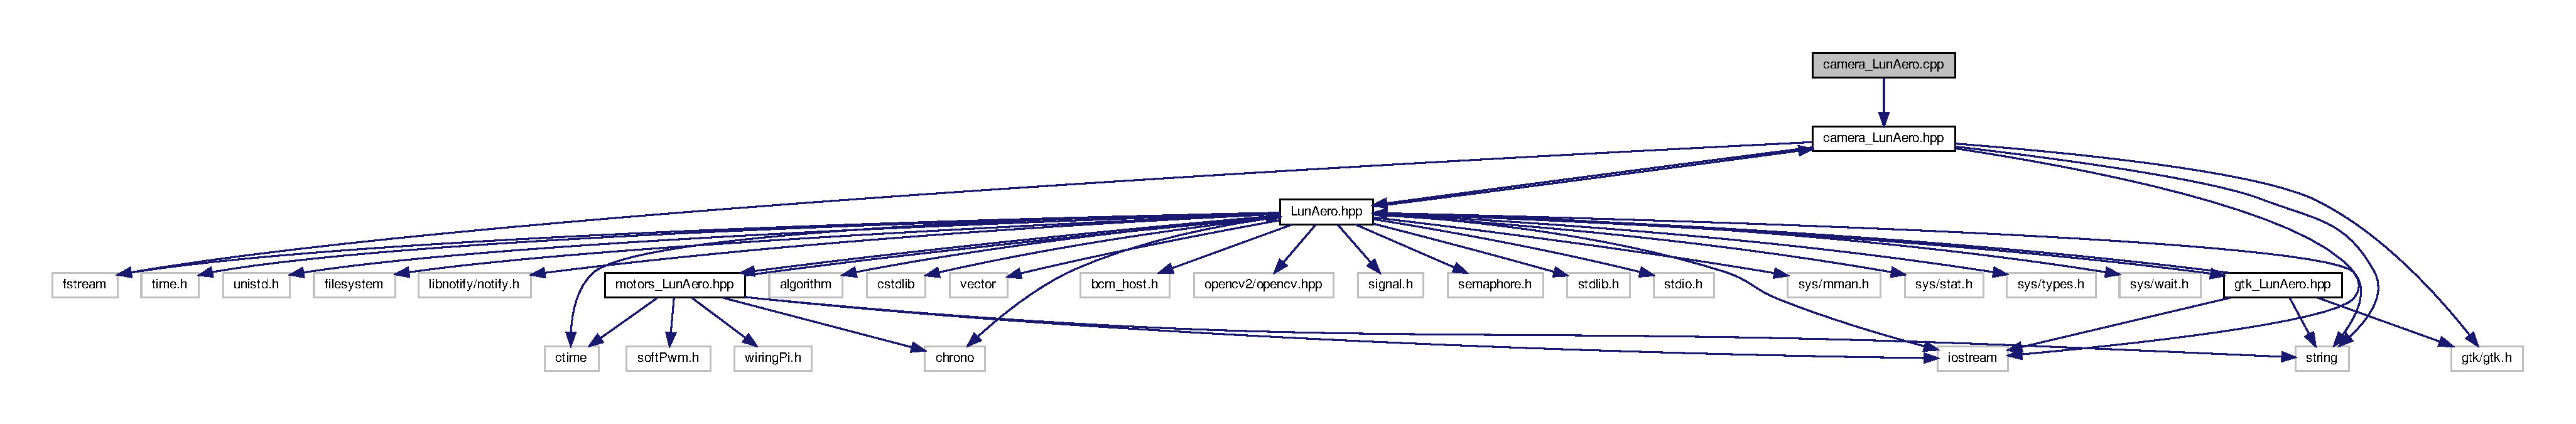
\includegraphics[width=350pt]{camera__LunAero_8cpp__incl}
\end{center}
\end{figure}
\subsection*{Functions}
\begin{DoxyCompactItemize}
\item 
int \hyperlink{camera__LunAero_8cpp_aa1ba49194500be6a8d8257f10bb98664}{confirm\+\_\+filespace} ()
\item 
int \hyperlink{camera__LunAero_8cpp_a04412b2d20fd79cb301ff78b67ece58b}{confirm\+\_\+mmal\+\_\+safety} (int error\+\_\+cnt)
\item 
void \hyperlink{camera__LunAero_8cpp_ae758d181371cae3622978bee489d5853}{camera\+\_\+start} ()
\item 
void \hyperlink{camera__LunAero_8cpp_a5828cc9ffb99db33b01fc641613cc59d}{camera\+\_\+preview} ()
\item 
std\+::string \hyperlink{camera__LunAero_8cpp_a7974714210bd0c046bfe4001f021697e}{command\+\_\+cam\+\_\+preview} ()
\item 
std\+::string \hyperlink{camera__LunAero_8cpp_aec581f7a0627d9324e87241671dcac8b}{command\+\_\+cam\+\_\+start} ()
\item 
void \hyperlink{camera__LunAero_8cpp_a02da38125ad204a1c0efc2355499d24c}{write\+\_\+video\+\_\+id} ()
\item 
void \hyperlink{camera__LunAero_8cpp_ac812e7b1a6d57e7ca306e001c99cf2b6}{first\+\_\+record} ()
\item 
void \hyperlink{camera__LunAero_8cpp_a36692fd7d4a8ab80af918d722a5b7a31}{reset\+\_\+record} ()
\item 
void \hyperlink{camera__LunAero_8cpp_add493d0baf9631379ba04e6690a3a8c8}{refresh\+\_\+camera} ()
\item 
void \hyperlink{camera__LunAero_8cpp_a988599eec44c71a7036263c3a7e817ce}{shutter\+\_\+up} ()
\item 
void \hyperlink{camera__LunAero_8cpp_a10580de6e0551da1e55d05ae761f3950}{shutter\+\_\+down} ()
\item 
void \hyperlink{camera__LunAero_8cpp_ac5f31346ed6951fa58b11f8e8e8a276a}{shutter\+\_\+up\+\_\+up} ()
\item 
void \hyperlink{camera__LunAero_8cpp_a527b79b0c862e105cc03bcac5ea85c84}{shutter\+\_\+down\+\_\+down} ()
\item 
void \hyperlink{camera__LunAero_8cpp_aa6d930952628ad620e2a259108de4b2c}{iso\+\_\+cycle} ()
\end{DoxyCompactItemize}


\subsection{Function Documentation}
\mbox{\Hypertarget{camera__LunAero_8cpp_a5828cc9ffb99db33b01fc641613cc59d}\label{camera__LunAero_8cpp_a5828cc9ffb99db33b01fc641613cc59d}} 
\index{camera\+\_\+\+Lun\+Aero.\+cpp@{camera\+\_\+\+Lun\+Aero.\+cpp}!camera\+\_\+preview@{camera\+\_\+preview}}
\index{camera\+\_\+preview@{camera\+\_\+preview}!camera\+\_\+\+Lun\+Aero.\+cpp@{camera\+\_\+\+Lun\+Aero.\+cpp}}
\subsubsection{\texorpdfstring{camera\+\_\+preview()}{camera\_preview()}}
{\footnotesize\ttfamily void camera\+\_\+preview (\begin{DoxyParamCaption}{ }\end{DoxyParamCaption})}

This command starts the preview screen using raspivid. The command is constructed based on command\+\_\+cam\+\_\+preview and the M\+M\+AL integrity is checked with mmal\+\_\+safety\+\_\+outcome. Here is the call graph for this function\+:
\nopagebreak
\begin{figure}[H]
\begin{center}
\leavevmode
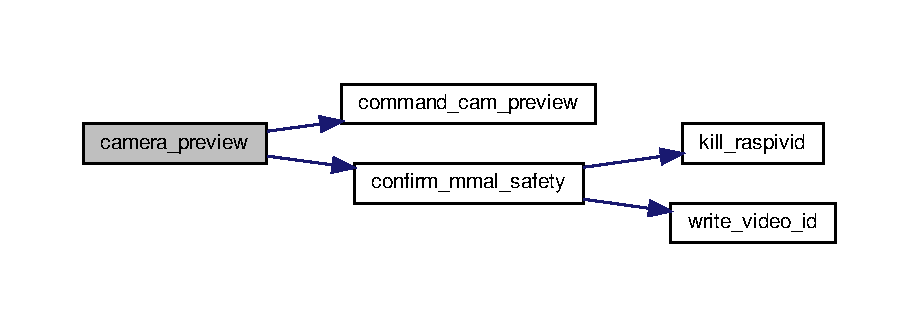
\includegraphics[width=350pt]{camera__LunAero_8cpp_a5828cc9ffb99db33b01fc641613cc59d_cgraph}
\end{center}
\end{figure}
Here is the caller graph for this function\+:
\nopagebreak
\begin{figure}[H]
\begin{center}
\leavevmode
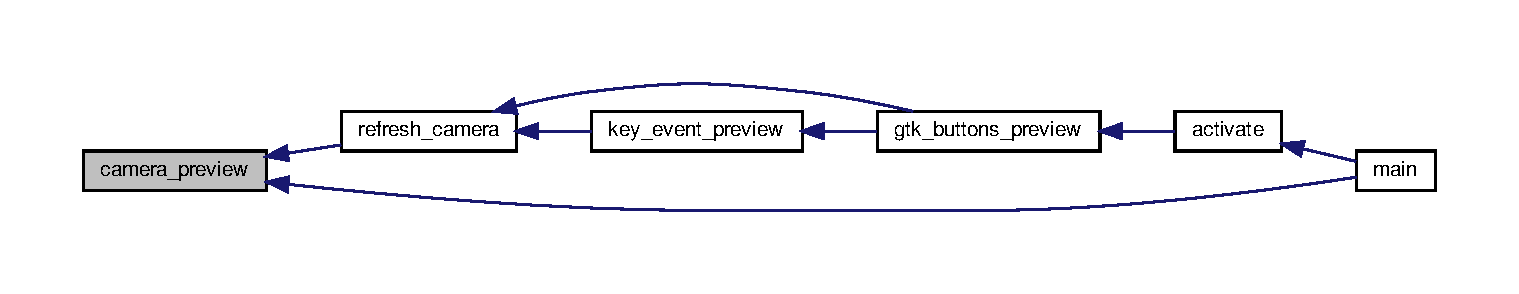
\includegraphics[width=350pt]{camera__LunAero_8cpp_a5828cc9ffb99db33b01fc641613cc59d_icgraph}
\end{center}
\end{figure}
\mbox{\Hypertarget{camera__LunAero_8cpp_ae758d181371cae3622978bee489d5853}\label{camera__LunAero_8cpp_ae758d181371cae3622978bee489d5853}} 
\index{camera\+\_\+\+Lun\+Aero.\+cpp@{camera\+\_\+\+Lun\+Aero.\+cpp}!camera\+\_\+start@{camera\+\_\+start}}
\index{camera\+\_\+start@{camera\+\_\+start}!camera\+\_\+\+Lun\+Aero.\+cpp@{camera\+\_\+\+Lun\+Aero.\+cpp}}
\subsubsection{\texorpdfstring{camera\+\_\+start()}{camera\_start()}}
{\footnotesize\ttfamily void camera\+\_\+start (\begin{DoxyParamCaption}{ }\end{DoxyParamCaption})}

This functions ties together multiple functions to 1) confirm\+\_\+filespace 2) confirm\+\_\+mmal\+\_\+safety 3) execute the command constructed by command\+\_\+cam\+\_\+start. Here is the call graph for this function\+:
\nopagebreak
\begin{figure}[H]
\begin{center}
\leavevmode
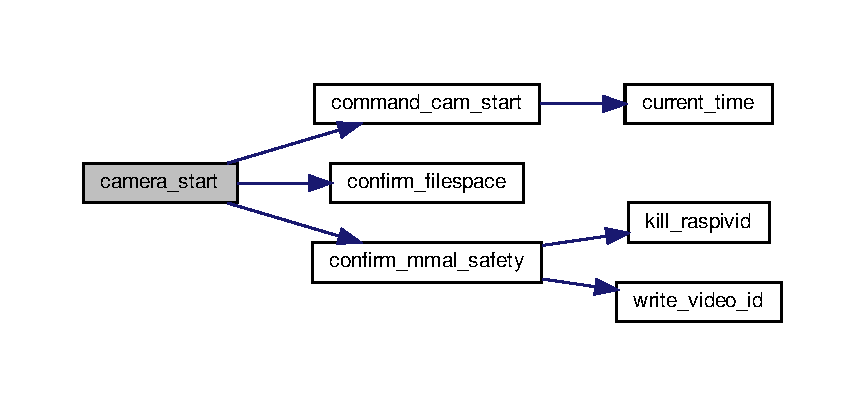
\includegraphics[width=350pt]{camera__LunAero_8cpp_ae758d181371cae3622978bee489d5853_cgraph}
\end{center}
\end{figure}
Here is the caller graph for this function\+:
\nopagebreak
\begin{figure}[H]
\begin{center}
\leavevmode
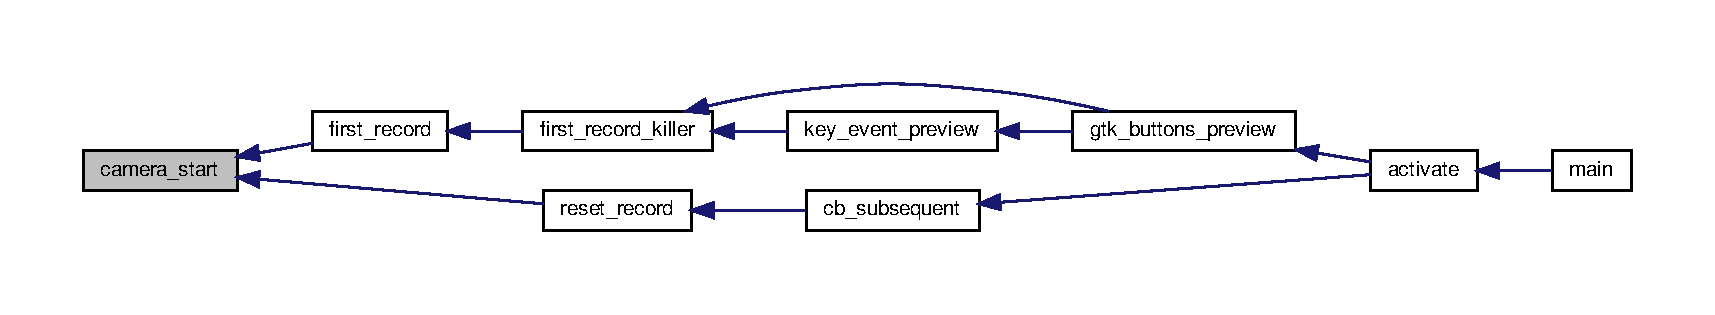
\includegraphics[width=350pt]{camera__LunAero_8cpp_ae758d181371cae3622978bee489d5853_icgraph}
\end{center}
\end{figure}
\mbox{\Hypertarget{camera__LunAero_8cpp_a7974714210bd0c046bfe4001f021697e}\label{camera__LunAero_8cpp_a7974714210bd0c046bfe4001f021697e}} 
\index{camera\+\_\+\+Lun\+Aero.\+cpp@{camera\+\_\+\+Lun\+Aero.\+cpp}!command\+\_\+cam\+\_\+preview@{command\+\_\+cam\+\_\+preview}}
\index{command\+\_\+cam\+\_\+preview@{command\+\_\+cam\+\_\+preview}!camera\+\_\+\+Lun\+Aero.\+cpp@{camera\+\_\+\+Lun\+Aero.\+cpp}}
\subsubsection{\texorpdfstring{command\+\_\+cam\+\_\+preview()}{command\_cam\_preview()}}
{\footnotesize\ttfamily std\+::string command\+\_\+cam\+\_\+preview (\begin{DoxyParamCaption}{ }\end{DoxyParamCaption})}

This function constructs the command string to call a raspivid preview. The size of the mini screen determined by other functions and used to construct the window.

\begin{DoxyReturn}{Returns}
commandstring the constructed command formatted as a string 
\end{DoxyReturn}
Here is the caller graph for this function\+:
\nopagebreak
\begin{figure}[H]
\begin{center}
\leavevmode
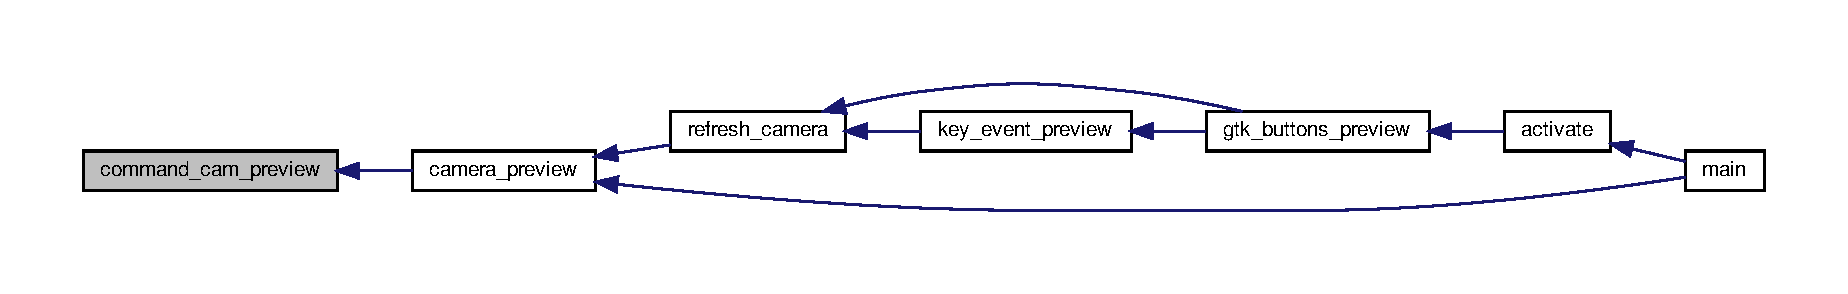
\includegraphics[width=350pt]{camera__LunAero_8cpp_a7974714210bd0c046bfe4001f021697e_icgraph}
\end{center}
\end{figure}
\mbox{\Hypertarget{camera__LunAero_8cpp_aec581f7a0627d9324e87241671dcac8b}\label{camera__LunAero_8cpp_aec581f7a0627d9324e87241671dcac8b}} 
\index{camera\+\_\+\+Lun\+Aero.\+cpp@{camera\+\_\+\+Lun\+Aero.\+cpp}!command\+\_\+cam\+\_\+start@{command\+\_\+cam\+\_\+start}}
\index{command\+\_\+cam\+\_\+start@{command\+\_\+cam\+\_\+start}!camera\+\_\+\+Lun\+Aero.\+cpp@{camera\+\_\+\+Lun\+Aero.\+cpp}}
\subsubsection{\texorpdfstring{command\+\_\+cam\+\_\+start()}{command\_cam\_start()}}
{\footnotesize\ttfamily std\+::string command\+\_\+cam\+\_\+start (\begin{DoxyParamCaption}{ }\end{DoxyParamCaption})}

This function constructs the command string to call a raspivid recording and preview window. The size of the mini screen determined by other functions and used to construct the preview window. The save location of the video is determined by the current timestamp.

\begin{DoxyReturn}{Returns}
commandstring the constructed command formatted as a string 
\end{DoxyReturn}
Here is the call graph for this function\+:
\nopagebreak
\begin{figure}[H]
\begin{center}
\leavevmode
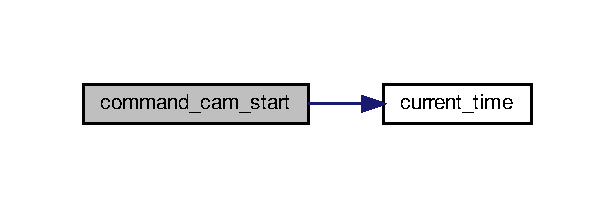
\includegraphics[width=295pt]{camera__LunAero_8cpp_aec581f7a0627d9324e87241671dcac8b_cgraph}
\end{center}
\end{figure}
Here is the caller graph for this function\+:
\nopagebreak
\begin{figure}[H]
\begin{center}
\leavevmode
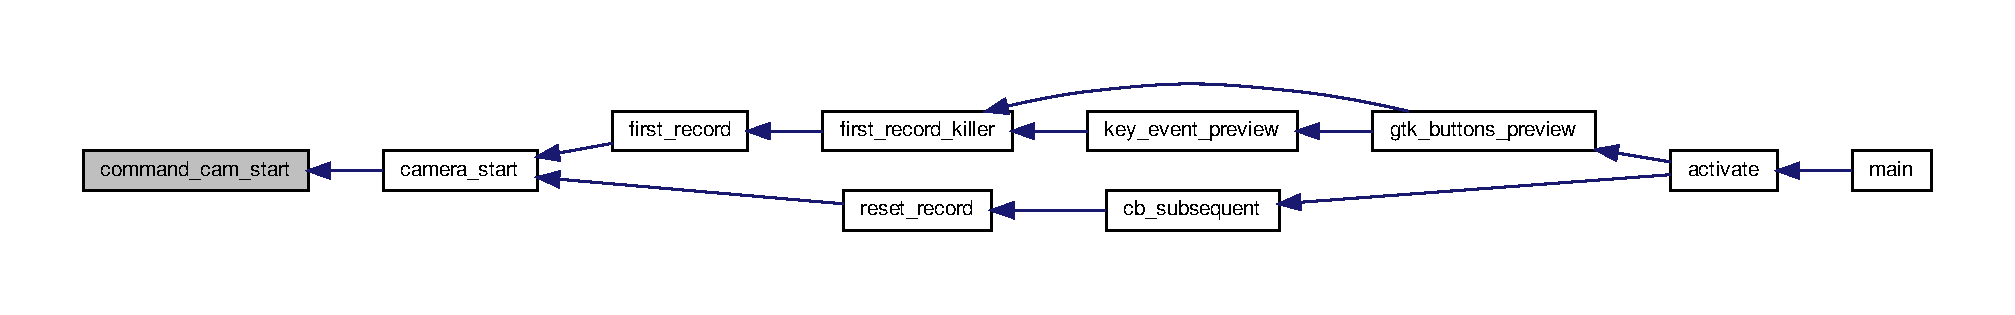
\includegraphics[width=350pt]{camera__LunAero_8cpp_aec581f7a0627d9324e87241671dcac8b_icgraph}
\end{center}
\end{figure}
\mbox{\Hypertarget{camera__LunAero_8cpp_aa1ba49194500be6a8d8257f10bb98664}\label{camera__LunAero_8cpp_aa1ba49194500be6a8d8257f10bb98664}} 
\index{camera\+\_\+\+Lun\+Aero.\+cpp@{camera\+\_\+\+Lun\+Aero.\+cpp}!confirm\+\_\+filespace@{confirm\+\_\+filespace}}
\index{confirm\+\_\+filespace@{confirm\+\_\+filespace}!camera\+\_\+\+Lun\+Aero.\+cpp@{camera\+\_\+\+Lun\+Aero.\+cpp}}
\subsubsection{\texorpdfstring{confirm\+\_\+filespace()}{confirm\_filespace()}}
{\footnotesize\ttfamily int confirm\+\_\+filespace (\begin{DoxyParamCaption}{ }\end{DoxyParamCaption})}

This function confirms that there is enought space on the output drive for a new video to be saved. While this is similar to \hyperlink{LunAero_8cpp}{Lun\+Aero.\+cpp}/startup\+\_\+disk\+\_\+check, it only checks the available space rather than the drive integrity. And, it does not predictively check for low hard drive space for future videos. If the check fails, a positive status is returned and the program ends.

\begin{DoxyReturn}{Returns}
status 
\end{DoxyReturn}
Here is the caller graph for this function\+:
\nopagebreak
\begin{figure}[H]
\begin{center}
\leavevmode
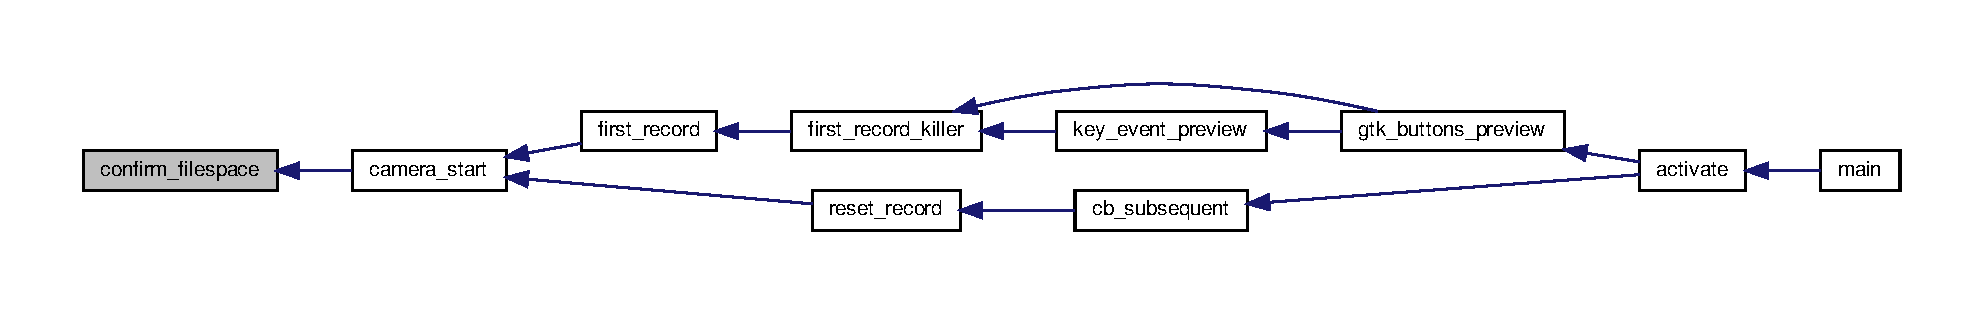
\includegraphics[width=350pt]{camera__LunAero_8cpp_aa1ba49194500be6a8d8257f10bb98664_icgraph}
\end{center}
\end{figure}
\mbox{\Hypertarget{camera__LunAero_8cpp_a04412b2d20fd79cb301ff78b67ece58b}\label{camera__LunAero_8cpp_a04412b2d20fd79cb301ff78b67ece58b}} 
\index{camera\+\_\+\+Lun\+Aero.\+cpp@{camera\+\_\+\+Lun\+Aero.\+cpp}!confirm\+\_\+mmal\+\_\+safety@{confirm\+\_\+mmal\+\_\+safety}}
\index{confirm\+\_\+mmal\+\_\+safety@{confirm\+\_\+mmal\+\_\+safety}!camera\+\_\+\+Lun\+Aero.\+cpp@{camera\+\_\+\+Lun\+Aero.\+cpp}}
\subsubsection{\texorpdfstring{confirm\+\_\+mmal\+\_\+safety()}{confirm\_mmal\_safety()}}
{\footnotesize\ttfamily int confirm\+\_\+mmal\+\_\+safety (\begin{DoxyParamCaption}\item[{int}]{error\+\_\+cnt }\end{DoxyParamCaption})}

This function checks the integrity of the M\+M\+AL camera connection. This prevents improper restarts of the raspivid program caused by quick successive stops and starts. Originally, on these restarts, the M\+M\+AL may fail for a few microseconds after a shutdown since something had not finished clearing in the background (black magic). This simply handles a few failures before deciding that the M\+M\+AL device is not actually connected and ending the program.

\begin{DoxyReturn}{Returns}
status 
\end{DoxyReturn}
Here is the call graph for this function\+:
\nopagebreak
\begin{figure}[H]
\begin{center}
\leavevmode
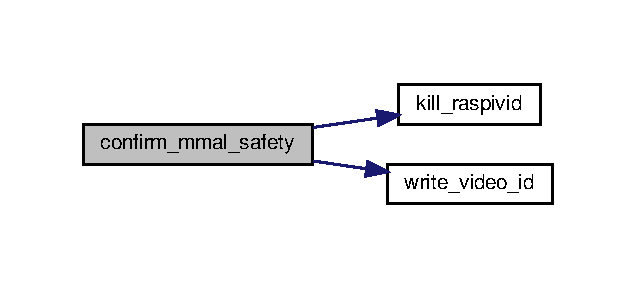
\includegraphics[width=305pt]{camera__LunAero_8cpp_a04412b2d20fd79cb301ff78b67ece58b_cgraph}
\end{center}
\end{figure}
Here is the caller graph for this function\+:
\nopagebreak
\begin{figure}[H]
\begin{center}
\leavevmode
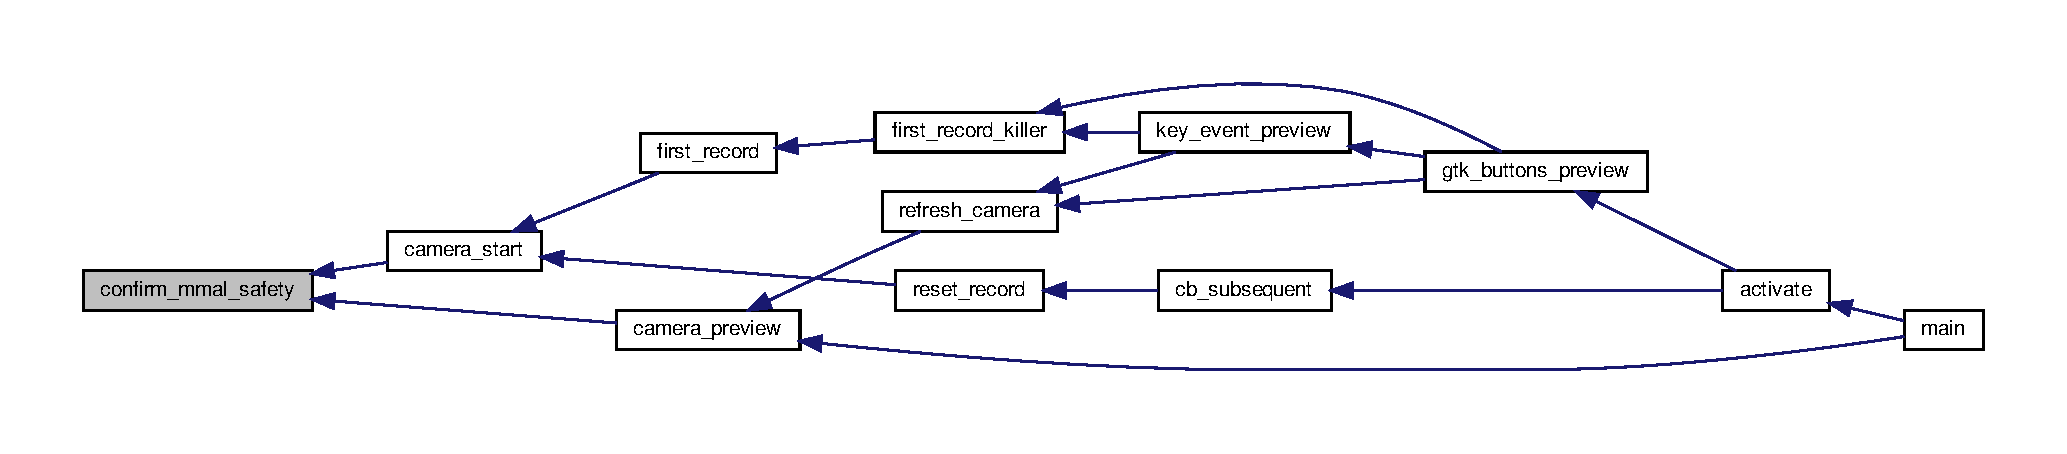
\includegraphics[width=350pt]{camera__LunAero_8cpp_a04412b2d20fd79cb301ff78b67ece58b_icgraph}
\end{center}
\end{figure}
\mbox{\Hypertarget{camera__LunAero_8cpp_ac812e7b1a6d57e7ca306e001c99cf2b6}\label{camera__LunAero_8cpp_ac812e7b1a6d57e7ca306e001c99cf2b6}} 
\index{camera\+\_\+\+Lun\+Aero.\+cpp@{camera\+\_\+\+Lun\+Aero.\+cpp}!first\+\_\+record@{first\+\_\+record}}
\index{first\+\_\+record@{first\+\_\+record}!camera\+\_\+\+Lun\+Aero.\+cpp@{camera\+\_\+\+Lun\+Aero.\+cpp}}
\subsubsection{\texorpdfstring{first\+\_\+record()}{first\_record()}}
{\footnotesize\ttfamily void first\+\_\+record (\begin{DoxyParamCaption}{ }\end{DoxyParamCaption})}

This function handles the first recording. This is distinct as we need to kill the preview window and ensure that the motors are in an initial state. If we don\textquotesingle{}t set the duty cycles for the motors to the minimum here, the motors start too aggressive and lose the target. Here is the call graph for this function\+:
\nopagebreak
\begin{figure}[H]
\begin{center}
\leavevmode
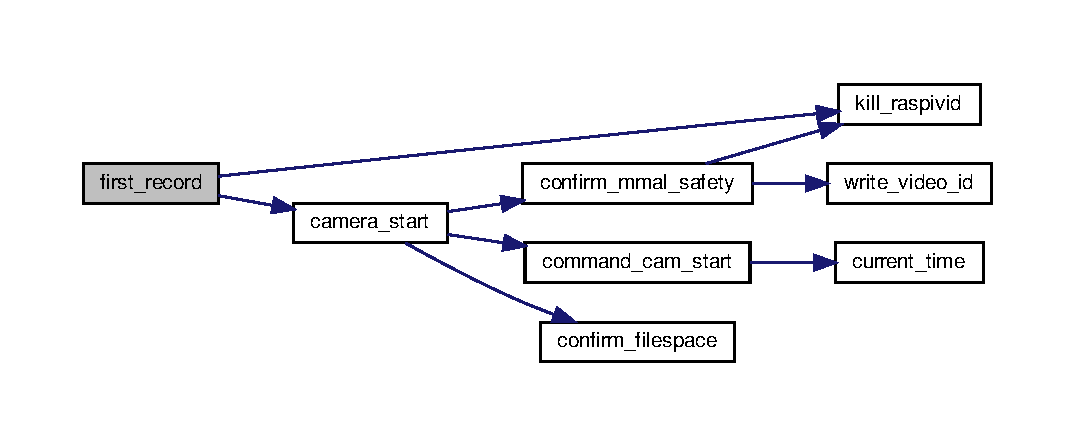
\includegraphics[width=350pt]{camera__LunAero_8cpp_ac812e7b1a6d57e7ca306e001c99cf2b6_cgraph}
\end{center}
\end{figure}
Here is the caller graph for this function\+:
\nopagebreak
\begin{figure}[H]
\begin{center}
\leavevmode
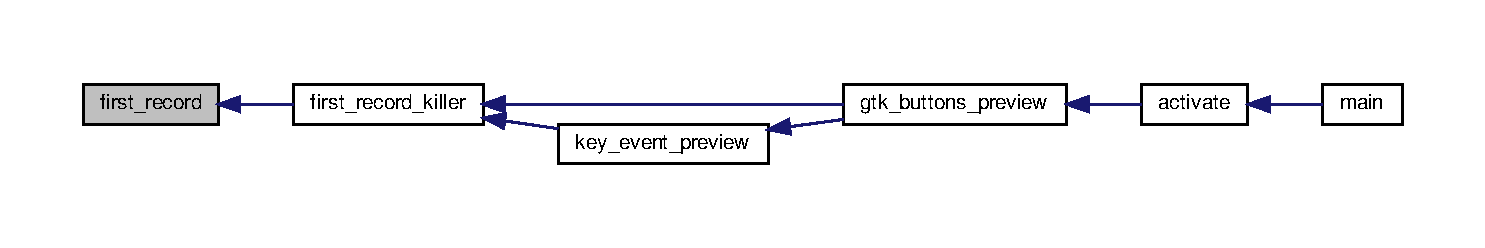
\includegraphics[width=350pt]{camera__LunAero_8cpp_ac812e7b1a6d57e7ca306e001c99cf2b6_icgraph}
\end{center}
\end{figure}
\mbox{\Hypertarget{camera__LunAero_8cpp_aa6d930952628ad620e2a259108de4b2c}\label{camera__LunAero_8cpp_aa6d930952628ad620e2a259108de4b2c}} 
\index{camera\+\_\+\+Lun\+Aero.\+cpp@{camera\+\_\+\+Lun\+Aero.\+cpp}!iso\+\_\+cycle@{iso\+\_\+cycle}}
\index{iso\+\_\+cycle@{iso\+\_\+cycle}!camera\+\_\+\+Lun\+Aero.\+cpp@{camera\+\_\+\+Lun\+Aero.\+cpp}}
\subsubsection{\texorpdfstring{iso\+\_\+cycle()}{iso\_cycle()}}
{\footnotesize\ttfamily void iso\+\_\+cycle (\begin{DoxyParamCaption}{ }\end{DoxyParamCaption})}

This function handles the I\+SO cycle from gtk\+\_\+\+Lun\+Aero. Since there are only 4 valid I\+SO values (100, 200, 400, 800) for the Raspberry Pi camera, it cycles through these values. Here is the caller graph for this function\+:
\nopagebreak
\begin{figure}[H]
\begin{center}
\leavevmode
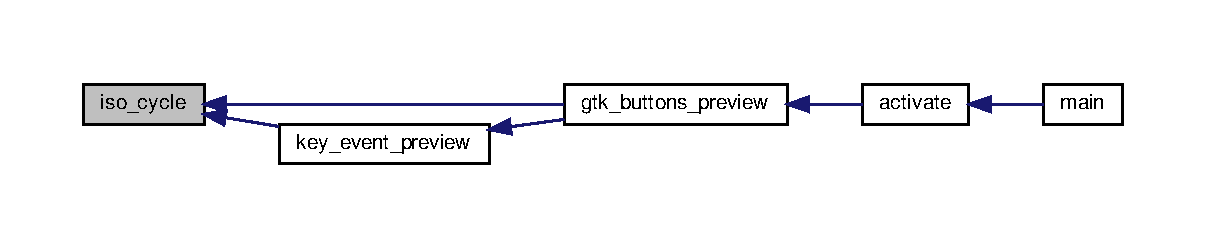
\includegraphics[width=350pt]{camera__LunAero_8cpp_aa6d930952628ad620e2a259108de4b2c_icgraph}
\end{center}
\end{figure}
\mbox{\Hypertarget{camera__LunAero_8cpp_add493d0baf9631379ba04e6690a3a8c8}\label{camera__LunAero_8cpp_add493d0baf9631379ba04e6690a3a8c8}} 
\index{camera\+\_\+\+Lun\+Aero.\+cpp@{camera\+\_\+\+Lun\+Aero.\+cpp}!refresh\+\_\+camera@{refresh\+\_\+camera}}
\index{refresh\+\_\+camera@{refresh\+\_\+camera}!camera\+\_\+\+Lun\+Aero.\+cpp@{camera\+\_\+\+Lun\+Aero.\+cpp}}
\subsubsection{\texorpdfstring{refresh\+\_\+camera()}{refresh\_camera()}}
{\footnotesize\ttfamily void refresh\+\_\+camera (\begin{DoxyParamCaption}{ }\end{DoxyParamCaption})}

This helper function is called by a G\+TK button and is used to kill the existing preview window and replace it with a new window based on the latest I\+S\+O/\+Shutter values. Here is the call graph for this function\+:
\nopagebreak
\begin{figure}[H]
\begin{center}
\leavevmode
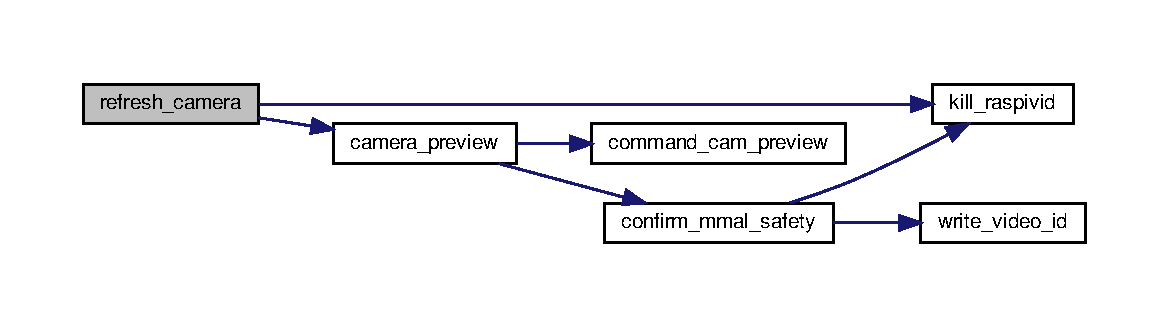
\includegraphics[width=350pt]{camera__LunAero_8cpp_add493d0baf9631379ba04e6690a3a8c8_cgraph}
\end{center}
\end{figure}
Here is the caller graph for this function\+:
\nopagebreak
\begin{figure}[H]
\begin{center}
\leavevmode
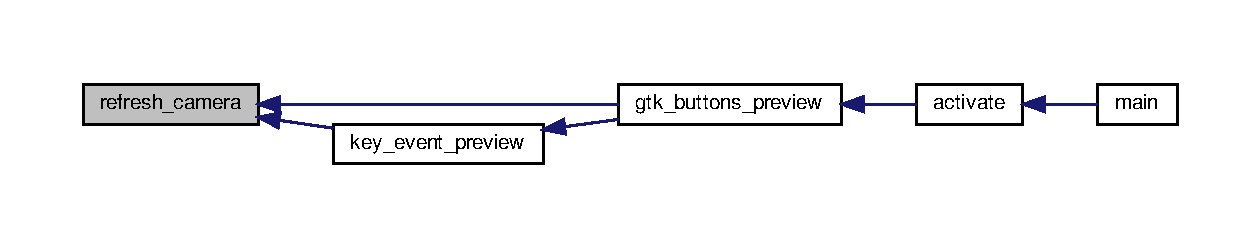
\includegraphics[width=350pt]{camera__LunAero_8cpp_add493d0baf9631379ba04e6690a3a8c8_icgraph}
\end{center}
\end{figure}
\mbox{\Hypertarget{camera__LunAero_8cpp_a36692fd7d4a8ab80af918d722a5b7a31}\label{camera__LunAero_8cpp_a36692fd7d4a8ab80af918d722a5b7a31}} 
\index{camera\+\_\+\+Lun\+Aero.\+cpp@{camera\+\_\+\+Lun\+Aero.\+cpp}!reset\+\_\+record@{reset\+\_\+record}}
\index{reset\+\_\+record@{reset\+\_\+record}!camera\+\_\+\+Lun\+Aero.\+cpp@{camera\+\_\+\+Lun\+Aero.\+cpp}}
\subsubsection{\texorpdfstring{reset\+\_\+record()}{reset\_record()}}
{\footnotesize\ttfamily void reset\+\_\+record (\begin{DoxyParamCaption}{ }\end{DoxyParamCaption})}

This helper function kills raspivid and starts recording for each video restart subsequent to the initial recording. Here is the call graph for this function\+:
\nopagebreak
\begin{figure}[H]
\begin{center}
\leavevmode
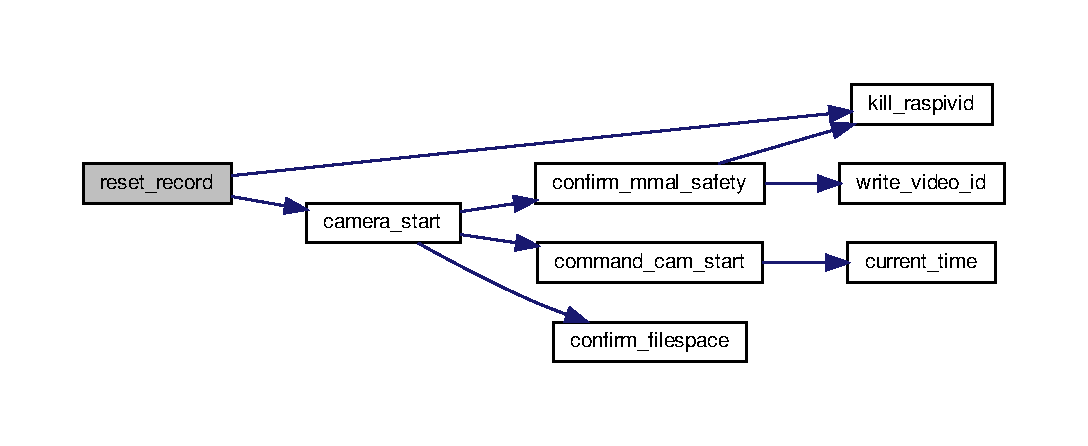
\includegraphics[width=350pt]{camera__LunAero_8cpp_a36692fd7d4a8ab80af918d722a5b7a31_cgraph}
\end{center}
\end{figure}
Here is the caller graph for this function\+:
\nopagebreak
\begin{figure}[H]
\begin{center}
\leavevmode
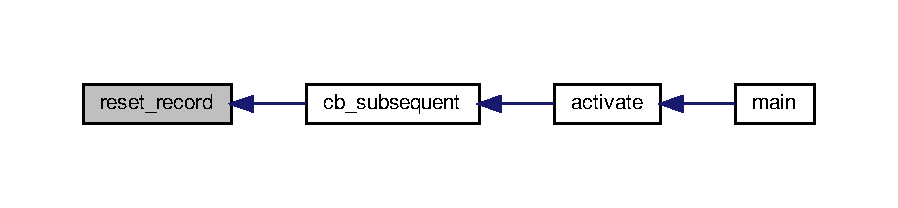
\includegraphics[width=350pt]{camera__LunAero_8cpp_a36692fd7d4a8ab80af918d722a5b7a31_icgraph}
\end{center}
\end{figure}
\mbox{\Hypertarget{camera__LunAero_8cpp_a10580de6e0551da1e55d05ae761f3950}\label{camera__LunAero_8cpp_a10580de6e0551da1e55d05ae761f3950}} 
\index{camera\+\_\+\+Lun\+Aero.\+cpp@{camera\+\_\+\+Lun\+Aero.\+cpp}!shutter\+\_\+down@{shutter\+\_\+down}}
\index{shutter\+\_\+down@{shutter\+\_\+down}!camera\+\_\+\+Lun\+Aero.\+cpp@{camera\+\_\+\+Lun\+Aero.\+cpp}}
\subsubsection{\texorpdfstring{shutter\+\_\+down()}{shutter\_down()}}
{\footnotesize\ttfamily void shutter\+\_\+down (\begin{DoxyParamCaption}{ }\end{DoxyParamCaption})}

This function called from gtk\+\_\+\+Lun\+Aero handles a request to decrease the shutter value. The minimum shutter value is locked in here and prevents a shutter value from extending below this limit. Here is the caller graph for this function\+:
\nopagebreak
\begin{figure}[H]
\begin{center}
\leavevmode
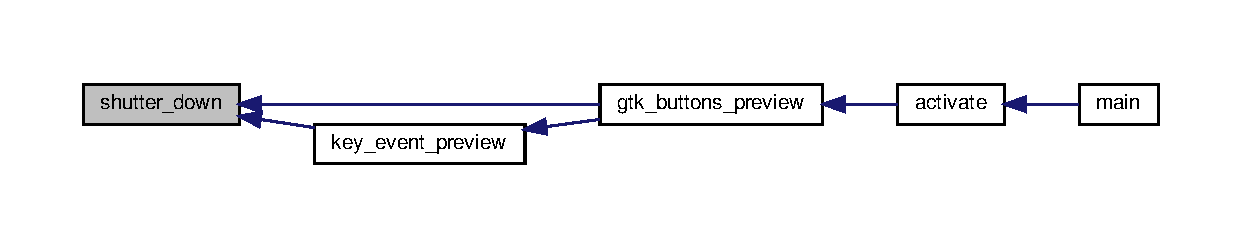
\includegraphics[width=350pt]{camera__LunAero_8cpp_a10580de6e0551da1e55d05ae761f3950_icgraph}
\end{center}
\end{figure}
\mbox{\Hypertarget{camera__LunAero_8cpp_a527b79b0c862e105cc03bcac5ea85c84}\label{camera__LunAero_8cpp_a527b79b0c862e105cc03bcac5ea85c84}} 
\index{camera\+\_\+\+Lun\+Aero.\+cpp@{camera\+\_\+\+Lun\+Aero.\+cpp}!shutter\+\_\+down\+\_\+down@{shutter\+\_\+down\+\_\+down}}
\index{shutter\+\_\+down\+\_\+down@{shutter\+\_\+down\+\_\+down}!camera\+\_\+\+Lun\+Aero.\+cpp@{camera\+\_\+\+Lun\+Aero.\+cpp}}
\subsubsection{\texorpdfstring{shutter\+\_\+down\+\_\+down()}{shutter\_down\_down()}}
{\footnotesize\ttfamily void shutter\+\_\+down\+\_\+down (\begin{DoxyParamCaption}{ }\end{DoxyParamCaption})}

This function called from gtk\+\_\+\+Lun\+Aero handles a request to greatly decrease the shutter value. The minimum shutter value is locked in here and prevents a shutter value from extending below this limit. Here is the caller graph for this function\+:
\nopagebreak
\begin{figure}[H]
\begin{center}
\leavevmode
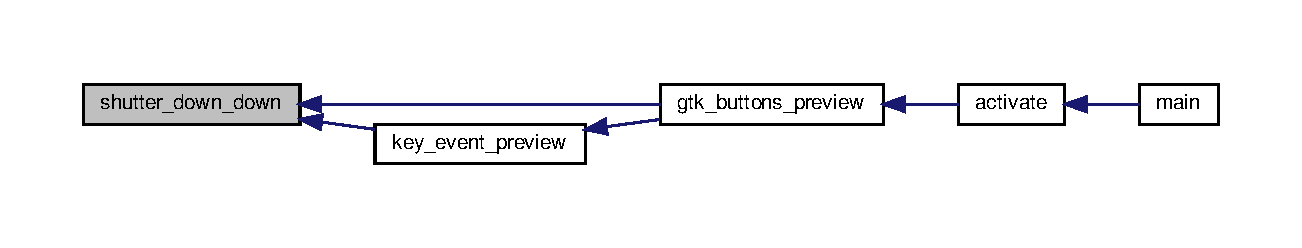
\includegraphics[width=350pt]{camera__LunAero_8cpp_a527b79b0c862e105cc03bcac5ea85c84_icgraph}
\end{center}
\end{figure}
\mbox{\Hypertarget{camera__LunAero_8cpp_a988599eec44c71a7036263c3a7e817ce}\label{camera__LunAero_8cpp_a988599eec44c71a7036263c3a7e817ce}} 
\index{camera\+\_\+\+Lun\+Aero.\+cpp@{camera\+\_\+\+Lun\+Aero.\+cpp}!shutter\+\_\+up@{shutter\+\_\+up}}
\index{shutter\+\_\+up@{shutter\+\_\+up}!camera\+\_\+\+Lun\+Aero.\+cpp@{camera\+\_\+\+Lun\+Aero.\+cpp}}
\subsubsection{\texorpdfstring{shutter\+\_\+up()}{shutter\_up()}}
{\footnotesize\ttfamily void shutter\+\_\+up (\begin{DoxyParamCaption}{ }\end{DoxyParamCaption})}

This function called from gtk\+\_\+\+Lun\+Aero handles a request to increase the shutter value. The maximum shutter value is locked in here and prevents a shutter value from extending beyond this limit. Here is the caller graph for this function\+:
\nopagebreak
\begin{figure}[H]
\begin{center}
\leavevmode
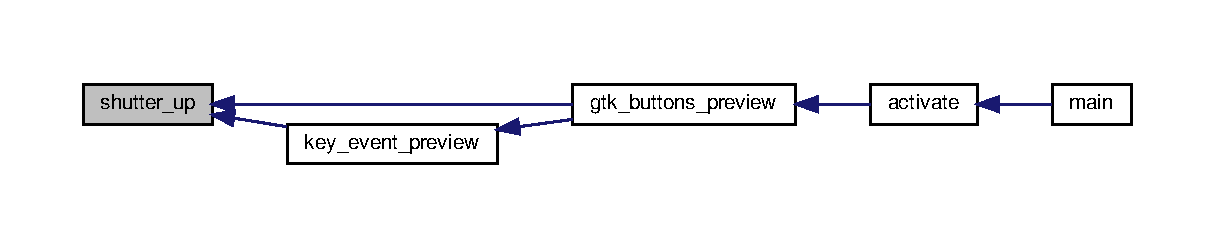
\includegraphics[width=350pt]{camera__LunAero_8cpp_a988599eec44c71a7036263c3a7e817ce_icgraph}
\end{center}
\end{figure}
\mbox{\Hypertarget{camera__LunAero_8cpp_ac5f31346ed6951fa58b11f8e8e8a276a}\label{camera__LunAero_8cpp_ac5f31346ed6951fa58b11f8e8e8a276a}} 
\index{camera\+\_\+\+Lun\+Aero.\+cpp@{camera\+\_\+\+Lun\+Aero.\+cpp}!shutter\+\_\+up\+\_\+up@{shutter\+\_\+up\+\_\+up}}
\index{shutter\+\_\+up\+\_\+up@{shutter\+\_\+up\+\_\+up}!camera\+\_\+\+Lun\+Aero.\+cpp@{camera\+\_\+\+Lun\+Aero.\+cpp}}
\subsubsection{\texorpdfstring{shutter\+\_\+up\+\_\+up()}{shutter\_up\_up()}}
{\footnotesize\ttfamily void shutter\+\_\+up\+\_\+up (\begin{DoxyParamCaption}{ }\end{DoxyParamCaption})}

This function called from gtk\+\_\+\+Lun\+Aero handles a request to greatly increase the shutter value. The maximum shutter value is locked in here and prevents a shutter value from extending beyond this limit. Here is the caller graph for this function\+:
\nopagebreak
\begin{figure}[H]
\begin{center}
\leavevmode
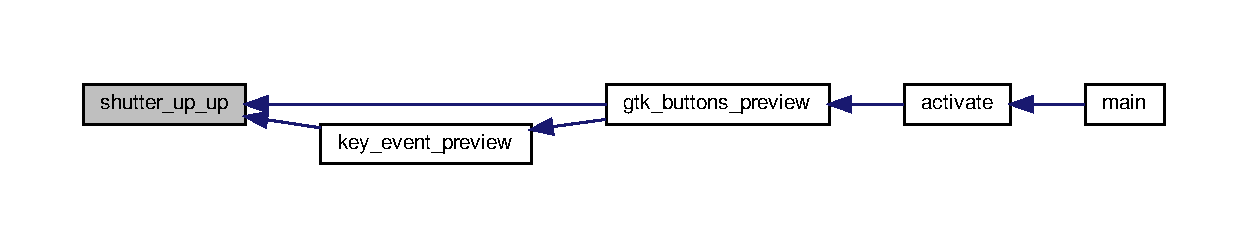
\includegraphics[width=350pt]{camera__LunAero_8cpp_ac5f31346ed6951fa58b11f8e8e8a276a_icgraph}
\end{center}
\end{figure}
\mbox{\Hypertarget{camera__LunAero_8cpp_a02da38125ad204a1c0efc2355499d24c}\label{camera__LunAero_8cpp_a02da38125ad204a1c0efc2355499d24c}} 
\index{camera\+\_\+\+Lun\+Aero.\+cpp@{camera\+\_\+\+Lun\+Aero.\+cpp}!write\+\_\+video\+\_\+id@{write\+\_\+video\+\_\+id}}
\index{write\+\_\+video\+\_\+id@{write\+\_\+video\+\_\+id}!camera\+\_\+\+Lun\+Aero.\+cpp@{camera\+\_\+\+Lun\+Aero.\+cpp}}
\subsubsection{\texorpdfstring{write\+\_\+video\+\_\+id()}{write\_video\_id()}}
{\footnotesize\ttfamily void write\+\_\+video\+\_\+id (\begin{DoxyParamCaption}{ }\end{DoxyParamCaption})}

This function creates a metadata file for each recording called by Lun\+Aero. The metadata includes the recording values set by the command constructed in command\+\_\+cam\+\_\+start. The file is stored in the same directory as the video. Here is the caller graph for this function\+:
\nopagebreak
\begin{figure}[H]
\begin{center}
\leavevmode
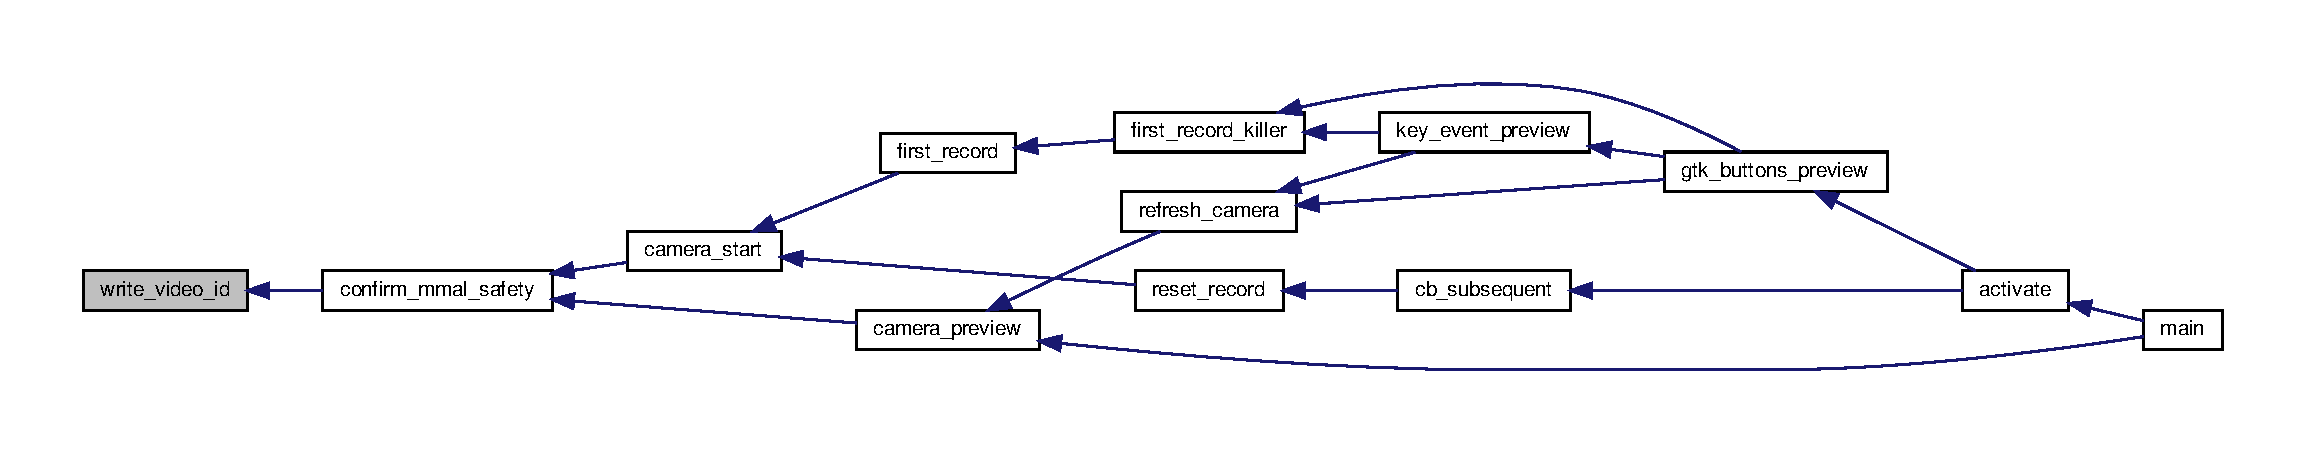
\includegraphics[width=350pt]{camera__LunAero_8cpp_a02da38125ad204a1c0efc2355499d24c_icgraph}
\end{center}
\end{figure}

\hypertarget{camera__LunAero_8hpp}{}\section{camera\+\_\+\+Lun\+Aero.\+hpp File Reference}
\label{camera__LunAero_8hpp}\index{camera\+\_\+\+Lun\+Aero.\+hpp@{camera\+\_\+\+Lun\+Aero.\+hpp}}
{\ttfamily \#include $<$string$>$}\newline
{\ttfamily \#include $<$iostream$>$}\newline
{\ttfamily \#include $<$gtk/gtk.\+h$>$}\newline
{\ttfamily \#include $<$fstream$>$}\newline
{\ttfamily \#include \char`\"{}Lun\+Aero.\+hpp\char`\"{}}\newline
Include dependency graph for camera\+\_\+\+Lun\+Aero.\+hpp\+:\nopagebreak
\begin{figure}[H]
\begin{center}
\leavevmode
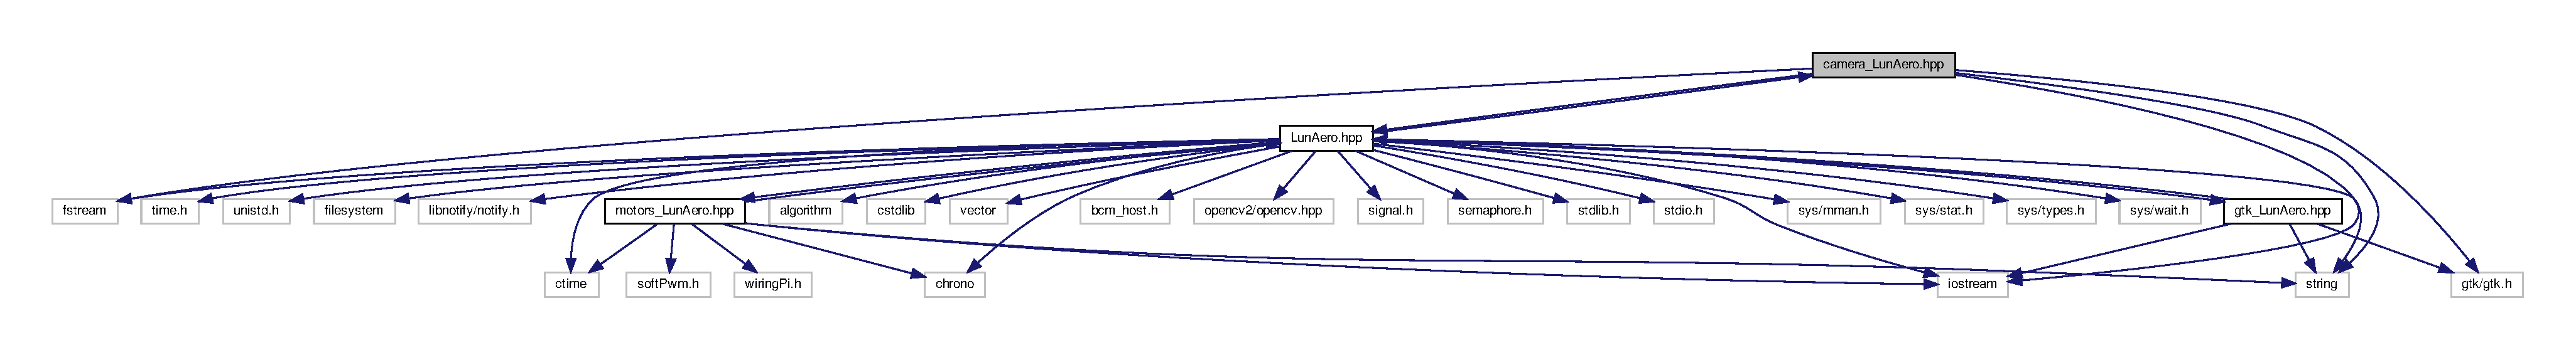
\includegraphics[width=350pt]{camera__LunAero_8hpp__incl}
\end{center}
\end{figure}
This graph shows which files directly or indirectly include this file\+:\nopagebreak
\begin{figure}[H]
\begin{center}
\leavevmode
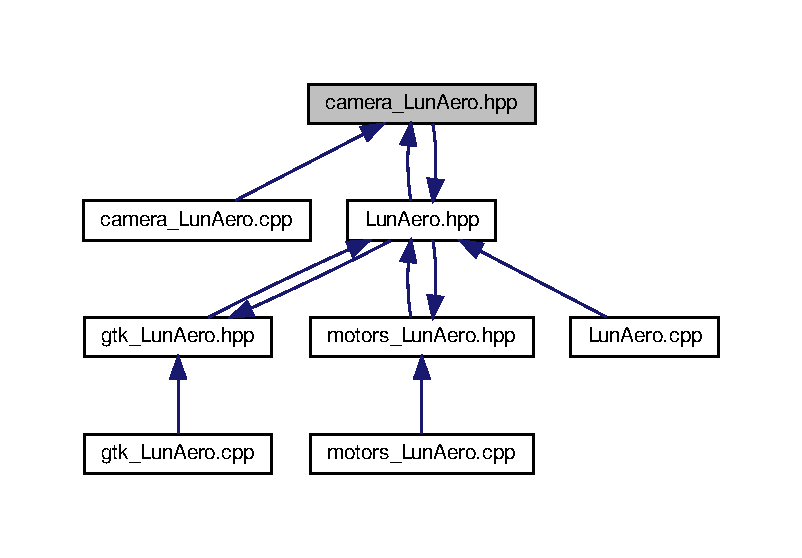
\includegraphics[width=350pt]{camera__LunAero_8hpp__dep__incl}
\end{center}
\end{figure}
\subsection*{Functions}
\begin{DoxyCompactItemize}
\item 
int \hyperlink{camera__LunAero_8hpp_aa1ba49194500be6a8d8257f10bb98664}{confirm\+\_\+filespace} ()
\item 
int \hyperlink{camera__LunAero_8hpp_a04412b2d20fd79cb301ff78b67ece58b}{confirm\+\_\+mmal\+\_\+safety} (int error\+\_\+cnt)
\item 
void \hyperlink{camera__LunAero_8hpp_a5828cc9ffb99db33b01fc641613cc59d}{camera\+\_\+preview} ()
\item 
void \hyperlink{camera__LunAero_8hpp_ae758d181371cae3622978bee489d5853}{camera\+\_\+start} ()
\item 
std\+::string \hyperlink{camera__LunAero_8hpp_aec581f7a0627d9324e87241671dcac8b}{command\+\_\+cam\+\_\+start} ()
\item 
std\+::string \hyperlink{camera__LunAero_8hpp_a7974714210bd0c046bfe4001f021697e}{command\+\_\+cam\+\_\+preview} ()
\item 
void \hyperlink{camera__LunAero_8hpp_a02da38125ad204a1c0efc2355499d24c}{write\+\_\+video\+\_\+id} ()
\item 
void \hyperlink{camera__LunAero_8hpp_aa6d930952628ad620e2a259108de4b2c}{iso\+\_\+cycle} ()
\item 
void \hyperlink{camera__LunAero_8hpp_ac812e7b1a6d57e7ca306e001c99cf2b6}{first\+\_\+record} ()
\item 
void \hyperlink{camera__LunAero_8hpp_add493d0baf9631379ba04e6690a3a8c8}{refresh\+\_\+camera} ()
\item 
void \hyperlink{camera__LunAero_8hpp_a988599eec44c71a7036263c3a7e817ce}{shutter\+\_\+up} ()
\item 
void \hyperlink{camera__LunAero_8hpp_a10580de6e0551da1e55d05ae761f3950}{shutter\+\_\+down} ()
\item 
void \hyperlink{camera__LunAero_8hpp_ac5f31346ed6951fa58b11f8e8e8a276a}{shutter\+\_\+up\+\_\+up} ()
\item 
void \hyperlink{camera__LunAero_8hpp_a527b79b0c862e105cc03bcac5ea85c84}{shutter\+\_\+down\+\_\+down} ()
\item 
void \hyperlink{camera__LunAero_8hpp_a36692fd7d4a8ab80af918d722a5b7a31}{reset\+\_\+record} ()
\end{DoxyCompactItemize}
\subsection*{Variables}
\begin{DoxyCompactItemize}
\item 
int \hyperlink{camera__LunAero_8hpp_adb112806aaf0c4ac7e5f142ad14cbf0e}{M\+M\+A\+L\+\_\+\+E\+R\+R\+O\+R\+\_\+\+T\+H\+R\+E\+SH} = 100
\item 
int \hyperlink{camera__LunAero_8hpp_a5934f6758956d58fc3ea68f9afecf4d5}{R\+P\+I\+\_\+\+F\+PS} = 30
\item 
int \hyperlink{camera__LunAero_8hpp_a111b596c8d8085e310d89ced7b3ce74e}{R\+P\+I\+\_\+\+BR} = 8000000
\item 
std\+::string \hyperlink{camera__LunAero_8hpp_a36c1dcc02f008386f600ee5024003d36}{R\+P\+I\+\_\+\+EX} = \char`\"{}auto\char`\"{}
\item 
int \hyperlink{camera__LunAero_8hpp_a5516a56b19d969ea808eeaf8d1c1da10}{S\+H\+U\+T\+\_\+\+J\+U\+MP} = 100
\item 
int \hyperlink{camera__LunAero_8hpp_a8b1e2a5d95b3018ff430d1a10ee3e8f2}{S\+H\+U\+T\+\_\+\+J\+U\+M\+P\+\_\+\+B\+IG} = 1000
\end{DoxyCompactItemize}


\subsection{Function Documentation}
\mbox{\Hypertarget{camera__LunAero_8hpp_a5828cc9ffb99db33b01fc641613cc59d}\label{camera__LunAero_8hpp_a5828cc9ffb99db33b01fc641613cc59d}} 
\index{camera\+\_\+\+Lun\+Aero.\+hpp@{camera\+\_\+\+Lun\+Aero.\+hpp}!camera\+\_\+preview@{camera\+\_\+preview}}
\index{camera\+\_\+preview@{camera\+\_\+preview}!camera\+\_\+\+Lun\+Aero.\+hpp@{camera\+\_\+\+Lun\+Aero.\+hpp}}
\subsubsection{\texorpdfstring{camera\+\_\+preview()}{camera\_preview()}}
{\footnotesize\ttfamily void camera\+\_\+preview (\begin{DoxyParamCaption}{ }\end{DoxyParamCaption})}

This command starts the preview screen using raspivid. The command is constructed based on command\+\_\+cam\+\_\+preview and the M\+M\+AL integrity is checked with mmal\+\_\+safety\+\_\+outcome. Here is the call graph for this function\+:\nopagebreak
\begin{figure}[H]
\begin{center}
\leavevmode
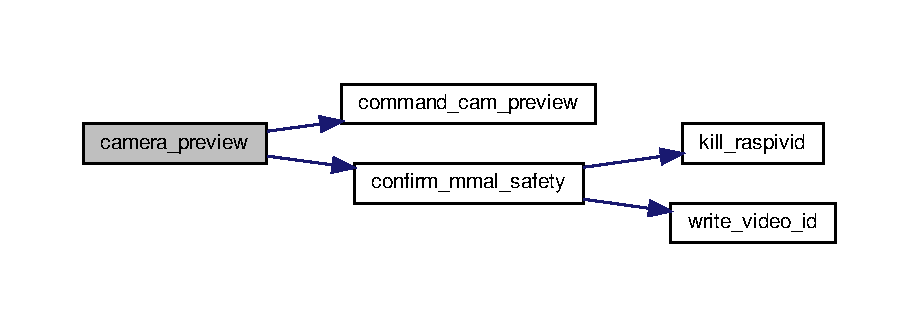
\includegraphics[width=350pt]{camera__LunAero_8hpp_a5828cc9ffb99db33b01fc641613cc59d_cgraph}
\end{center}
\end{figure}
Here is the caller graph for this function\+:\nopagebreak
\begin{figure}[H]
\begin{center}
\leavevmode
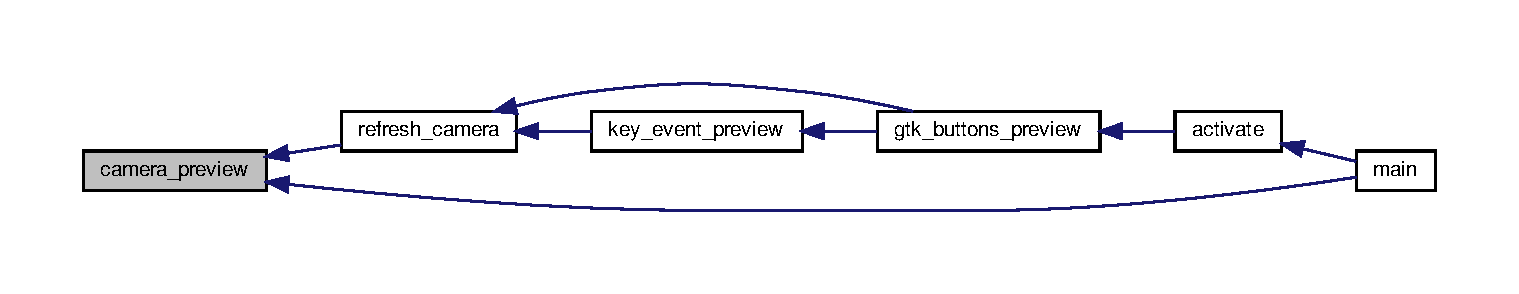
\includegraphics[width=350pt]{camera__LunAero_8hpp_a5828cc9ffb99db33b01fc641613cc59d_icgraph}
\end{center}
\end{figure}
\mbox{\Hypertarget{camera__LunAero_8hpp_ae758d181371cae3622978bee489d5853}\label{camera__LunAero_8hpp_ae758d181371cae3622978bee489d5853}} 
\index{camera\+\_\+\+Lun\+Aero.\+hpp@{camera\+\_\+\+Lun\+Aero.\+hpp}!camera\+\_\+start@{camera\+\_\+start}}
\index{camera\+\_\+start@{camera\+\_\+start}!camera\+\_\+\+Lun\+Aero.\+hpp@{camera\+\_\+\+Lun\+Aero.\+hpp}}
\subsubsection{\texorpdfstring{camera\+\_\+start()}{camera\_start()}}
{\footnotesize\ttfamily void camera\+\_\+start (\begin{DoxyParamCaption}{ }\end{DoxyParamCaption})}

This functions ties together multiple functions to 1) confirm\+\_\+filespace 2) confirm\+\_\+mmal\+\_\+safety 3) execute the command constructed by command\+\_\+cam\+\_\+start. Here is the call graph for this function\+:\nopagebreak
\begin{figure}[H]
\begin{center}
\leavevmode
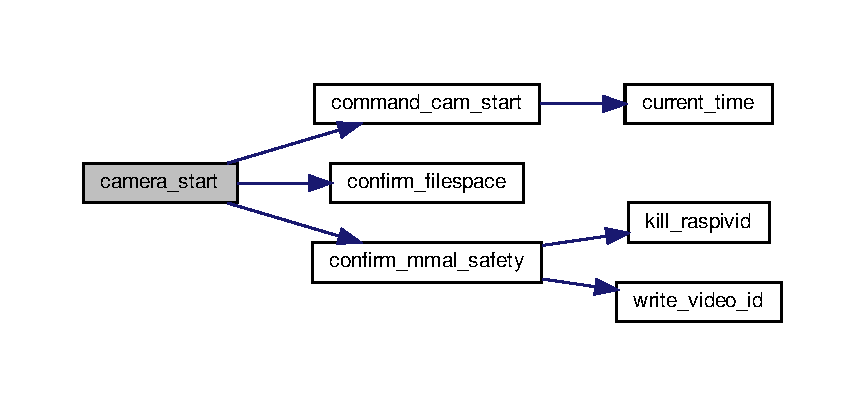
\includegraphics[width=350pt]{camera__LunAero_8hpp_ae758d181371cae3622978bee489d5853_cgraph}
\end{center}
\end{figure}
Here is the caller graph for this function\+:\nopagebreak
\begin{figure}[H]
\begin{center}
\leavevmode
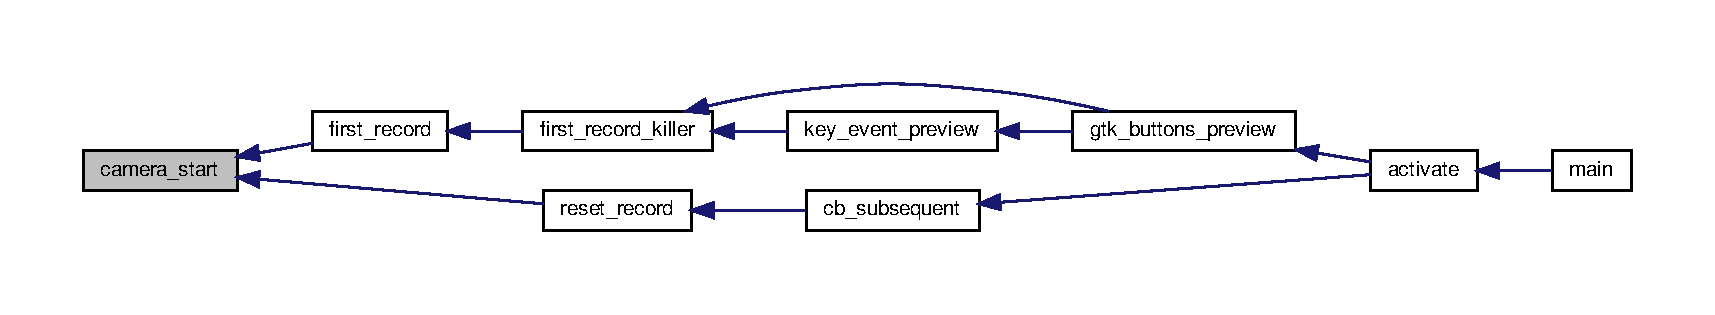
\includegraphics[width=350pt]{camera__LunAero_8hpp_ae758d181371cae3622978bee489d5853_icgraph}
\end{center}
\end{figure}
\mbox{\Hypertarget{camera__LunAero_8hpp_a7974714210bd0c046bfe4001f021697e}\label{camera__LunAero_8hpp_a7974714210bd0c046bfe4001f021697e}} 
\index{camera\+\_\+\+Lun\+Aero.\+hpp@{camera\+\_\+\+Lun\+Aero.\+hpp}!command\+\_\+cam\+\_\+preview@{command\+\_\+cam\+\_\+preview}}
\index{command\+\_\+cam\+\_\+preview@{command\+\_\+cam\+\_\+preview}!camera\+\_\+\+Lun\+Aero.\+hpp@{camera\+\_\+\+Lun\+Aero.\+hpp}}
\subsubsection{\texorpdfstring{command\+\_\+cam\+\_\+preview()}{command\_cam\_preview()}}
{\footnotesize\ttfamily std\+::string command\+\_\+cam\+\_\+preview (\begin{DoxyParamCaption}{ }\end{DoxyParamCaption})}

This function constructs the command string to call a raspivid preview. The size of the mini screen determined by other functions and used to construct the window.

\begin{DoxyReturn}{Returns}
commandstring the constructed command formatted as a string 
\end{DoxyReturn}
Here is the caller graph for this function\+:\nopagebreak
\begin{figure}[H]
\begin{center}
\leavevmode
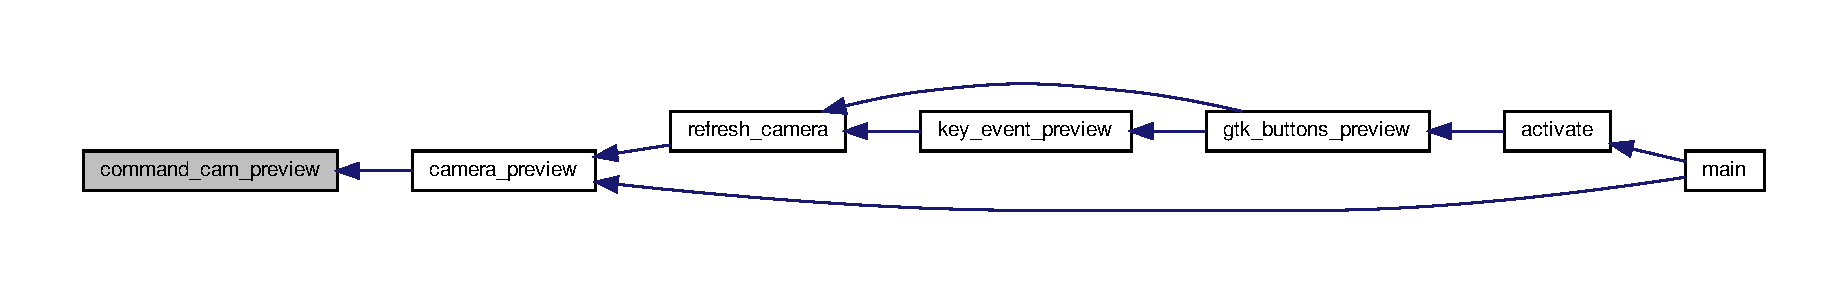
\includegraphics[width=350pt]{camera__LunAero_8hpp_a7974714210bd0c046bfe4001f021697e_icgraph}
\end{center}
\end{figure}
\mbox{\Hypertarget{camera__LunAero_8hpp_aec581f7a0627d9324e87241671dcac8b}\label{camera__LunAero_8hpp_aec581f7a0627d9324e87241671dcac8b}} 
\index{camera\+\_\+\+Lun\+Aero.\+hpp@{camera\+\_\+\+Lun\+Aero.\+hpp}!command\+\_\+cam\+\_\+start@{command\+\_\+cam\+\_\+start}}
\index{command\+\_\+cam\+\_\+start@{command\+\_\+cam\+\_\+start}!camera\+\_\+\+Lun\+Aero.\+hpp@{camera\+\_\+\+Lun\+Aero.\+hpp}}
\subsubsection{\texorpdfstring{command\+\_\+cam\+\_\+start()}{command\_cam\_start()}}
{\footnotesize\ttfamily std\+::string command\+\_\+cam\+\_\+start (\begin{DoxyParamCaption}{ }\end{DoxyParamCaption})}

This function constructs the command string to call a raspivid recording and preview window. The size of the mini screen determined by other functions and used to construct the preview window. The save location of the video is determined by the current timestamp.

\begin{DoxyReturn}{Returns}
commandstring the constructed command formatted as a string 
\end{DoxyReturn}
Here is the call graph for this function\+:\nopagebreak
\begin{figure}[H]
\begin{center}
\leavevmode
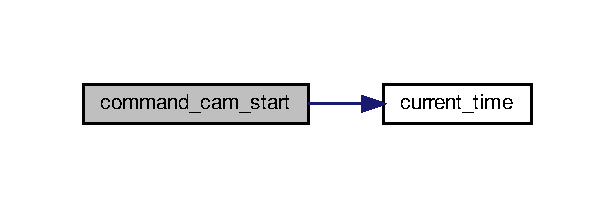
\includegraphics[width=295pt]{camera__LunAero_8hpp_aec581f7a0627d9324e87241671dcac8b_cgraph}
\end{center}
\end{figure}
Here is the caller graph for this function\+:\nopagebreak
\begin{figure}[H]
\begin{center}
\leavevmode
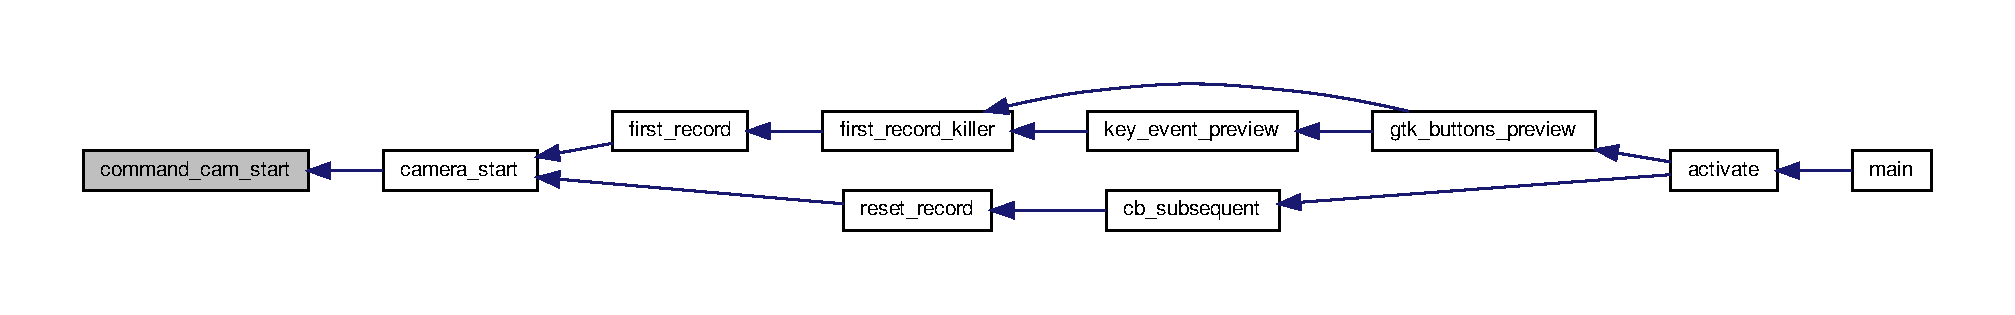
\includegraphics[width=350pt]{camera__LunAero_8hpp_aec581f7a0627d9324e87241671dcac8b_icgraph}
\end{center}
\end{figure}
\mbox{\Hypertarget{camera__LunAero_8hpp_aa1ba49194500be6a8d8257f10bb98664}\label{camera__LunAero_8hpp_aa1ba49194500be6a8d8257f10bb98664}} 
\index{camera\+\_\+\+Lun\+Aero.\+hpp@{camera\+\_\+\+Lun\+Aero.\+hpp}!confirm\+\_\+filespace@{confirm\+\_\+filespace}}
\index{confirm\+\_\+filespace@{confirm\+\_\+filespace}!camera\+\_\+\+Lun\+Aero.\+hpp@{camera\+\_\+\+Lun\+Aero.\+hpp}}
\subsubsection{\texorpdfstring{confirm\+\_\+filespace()}{confirm\_filespace()}}
{\footnotesize\ttfamily int confirm\+\_\+filespace (\begin{DoxyParamCaption}{ }\end{DoxyParamCaption})}

This function confirms that there is enought space on the output drive for a new video to be saved. While this is similar to \hyperlink{LunAero_8cpp}{Lun\+Aero.\+cpp}/startup\+\_\+disk\+\_\+check, it only checks the available space rather than the drive integrity. And, it does not predictively check for low hard drive space for future videos. If the check fails, a positive status is returned and the program ends.

\begin{DoxyReturn}{Returns}
status 
\end{DoxyReturn}
Here is the caller graph for this function\+:\nopagebreak
\begin{figure}[H]
\begin{center}
\leavevmode
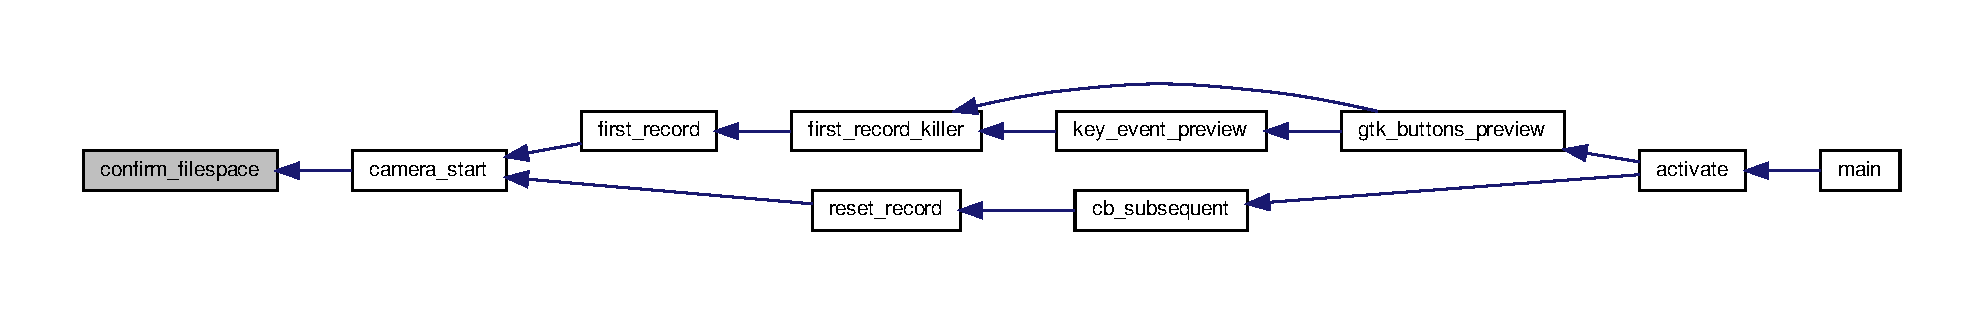
\includegraphics[width=350pt]{camera__LunAero_8hpp_aa1ba49194500be6a8d8257f10bb98664_icgraph}
\end{center}
\end{figure}
\mbox{\Hypertarget{camera__LunAero_8hpp_a04412b2d20fd79cb301ff78b67ece58b}\label{camera__LunAero_8hpp_a04412b2d20fd79cb301ff78b67ece58b}} 
\index{camera\+\_\+\+Lun\+Aero.\+hpp@{camera\+\_\+\+Lun\+Aero.\+hpp}!confirm\+\_\+mmal\+\_\+safety@{confirm\+\_\+mmal\+\_\+safety}}
\index{confirm\+\_\+mmal\+\_\+safety@{confirm\+\_\+mmal\+\_\+safety}!camera\+\_\+\+Lun\+Aero.\+hpp@{camera\+\_\+\+Lun\+Aero.\+hpp}}
\subsubsection{\texorpdfstring{confirm\+\_\+mmal\+\_\+safety()}{confirm\_mmal\_safety()}}
{\footnotesize\ttfamily int confirm\+\_\+mmal\+\_\+safety (\begin{DoxyParamCaption}\item[{int}]{error\+\_\+cnt }\end{DoxyParamCaption})}

This function checks the integrity of the M\+M\+AL camera connection. This prevents improper restarts of the raspivid program caused by quick successive stops and starts. Originally, on these restarts, the M\+M\+AL may fail for a few microseconds after a shutdown since something had not finished clearing in the background (black magic). This simply handles a few failures before deciding that the M\+M\+AL device is not actually connected and ending the program.

\begin{DoxyReturn}{Returns}
status 
\end{DoxyReturn}
Here is the call graph for this function\+:\nopagebreak
\begin{figure}[H]
\begin{center}
\leavevmode
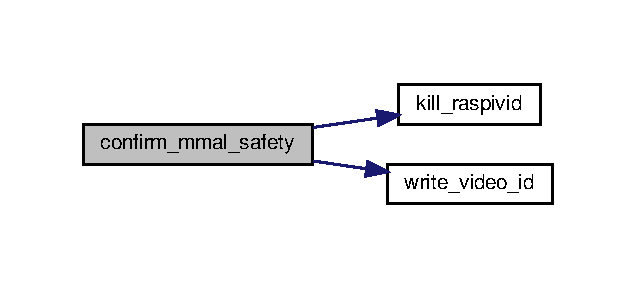
\includegraphics[width=305pt]{camera__LunAero_8hpp_a04412b2d20fd79cb301ff78b67ece58b_cgraph}
\end{center}
\end{figure}
Here is the caller graph for this function\+:\nopagebreak
\begin{figure}[H]
\begin{center}
\leavevmode
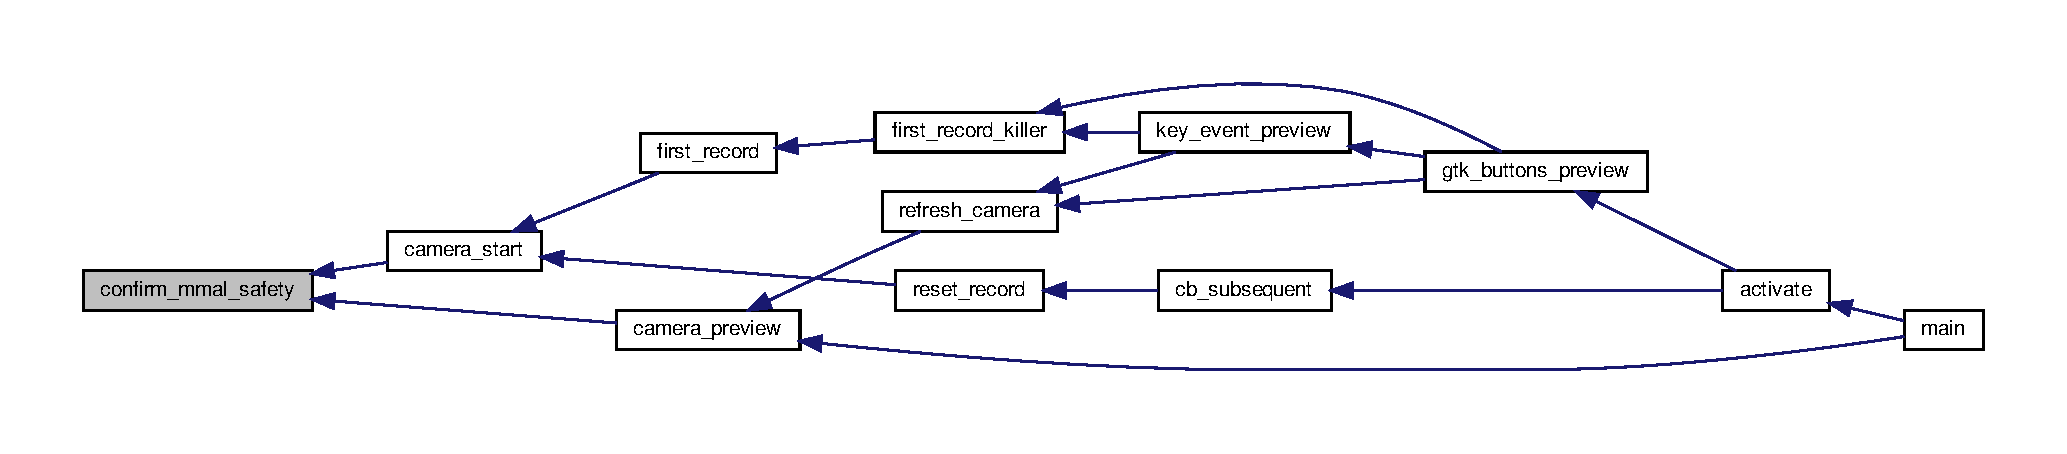
\includegraphics[width=350pt]{camera__LunAero_8hpp_a04412b2d20fd79cb301ff78b67ece58b_icgraph}
\end{center}
\end{figure}
\mbox{\Hypertarget{camera__LunAero_8hpp_ac812e7b1a6d57e7ca306e001c99cf2b6}\label{camera__LunAero_8hpp_ac812e7b1a6d57e7ca306e001c99cf2b6}} 
\index{camera\+\_\+\+Lun\+Aero.\+hpp@{camera\+\_\+\+Lun\+Aero.\+hpp}!first\+\_\+record@{first\+\_\+record}}
\index{first\+\_\+record@{first\+\_\+record}!camera\+\_\+\+Lun\+Aero.\+hpp@{camera\+\_\+\+Lun\+Aero.\+hpp}}
\subsubsection{\texorpdfstring{first\+\_\+record()}{first\_record()}}
{\footnotesize\ttfamily void first\+\_\+record (\begin{DoxyParamCaption}{ }\end{DoxyParamCaption})}

This function handles the first recording. This is distinct as we need to kill the preview window and ensure that the motors are in an initial state. If we don\textquotesingle{}t set the duty cycles for the motors to the minimum here, the motors start too aggressive and lose the target. Here is the call graph for this function\+:\nopagebreak
\begin{figure}[H]
\begin{center}
\leavevmode
\includegraphics[width=350pt]{camera__LunAero_8hpp_ac812e7b1a6d57e7ca306e001c99cf2b6_cgraph}
\end{center}
\end{figure}
Here is the caller graph for this function\+:\nopagebreak
\begin{figure}[H]
\begin{center}
\leavevmode
\includegraphics[width=350pt]{camera__LunAero_8hpp_ac812e7b1a6d57e7ca306e001c99cf2b6_icgraph}
\end{center}
\end{figure}
\mbox{\Hypertarget{camera__LunAero_8hpp_aa6d930952628ad620e2a259108de4b2c}\label{camera__LunAero_8hpp_aa6d930952628ad620e2a259108de4b2c}} 
\index{camera\+\_\+\+Lun\+Aero.\+hpp@{camera\+\_\+\+Lun\+Aero.\+hpp}!iso\+\_\+cycle@{iso\+\_\+cycle}}
\index{iso\+\_\+cycle@{iso\+\_\+cycle}!camera\+\_\+\+Lun\+Aero.\+hpp@{camera\+\_\+\+Lun\+Aero.\+hpp}}
\subsubsection{\texorpdfstring{iso\+\_\+cycle()}{iso\_cycle()}}
{\footnotesize\ttfamily void iso\+\_\+cycle (\begin{DoxyParamCaption}{ }\end{DoxyParamCaption})}

This function handles the I\+SO cycle from gtk\+\_\+\+Lun\+Aero. Since there are only 4 valid I\+SO values (100, 200, 400, 800) for the Raspberry Pi camera, it cycles through these values. Here is the caller graph for this function\+:\nopagebreak
\begin{figure}[H]
\begin{center}
\leavevmode
\includegraphics[width=350pt]{camera__LunAero_8hpp_aa6d930952628ad620e2a259108de4b2c_icgraph}
\end{center}
\end{figure}
\mbox{\Hypertarget{camera__LunAero_8hpp_add493d0baf9631379ba04e6690a3a8c8}\label{camera__LunAero_8hpp_add493d0baf9631379ba04e6690a3a8c8}} 
\index{camera\+\_\+\+Lun\+Aero.\+hpp@{camera\+\_\+\+Lun\+Aero.\+hpp}!refresh\+\_\+camera@{refresh\+\_\+camera}}
\index{refresh\+\_\+camera@{refresh\+\_\+camera}!camera\+\_\+\+Lun\+Aero.\+hpp@{camera\+\_\+\+Lun\+Aero.\+hpp}}
\subsubsection{\texorpdfstring{refresh\+\_\+camera()}{refresh\_camera()}}
{\footnotesize\ttfamily void refresh\+\_\+camera (\begin{DoxyParamCaption}{ }\end{DoxyParamCaption})}

This helper function is called by a G\+TK button and is used to kill the existing preview window and replace it with a new window based on the latest I\+S\+O/\+Shutter values. Here is the call graph for this function\+:\nopagebreak
\begin{figure}[H]
\begin{center}
\leavevmode
\includegraphics[width=350pt]{camera__LunAero_8hpp_add493d0baf9631379ba04e6690a3a8c8_cgraph}
\end{center}
\end{figure}
Here is the caller graph for this function\+:\nopagebreak
\begin{figure}[H]
\begin{center}
\leavevmode
\includegraphics[width=350pt]{camera__LunAero_8hpp_add493d0baf9631379ba04e6690a3a8c8_icgraph}
\end{center}
\end{figure}
\mbox{\Hypertarget{camera__LunAero_8hpp_a36692fd7d4a8ab80af918d722a5b7a31}\label{camera__LunAero_8hpp_a36692fd7d4a8ab80af918d722a5b7a31}} 
\index{camera\+\_\+\+Lun\+Aero.\+hpp@{camera\+\_\+\+Lun\+Aero.\+hpp}!reset\+\_\+record@{reset\+\_\+record}}
\index{reset\+\_\+record@{reset\+\_\+record}!camera\+\_\+\+Lun\+Aero.\+hpp@{camera\+\_\+\+Lun\+Aero.\+hpp}}
\subsubsection{\texorpdfstring{reset\+\_\+record()}{reset\_record()}}
{\footnotesize\ttfamily void reset\+\_\+record (\begin{DoxyParamCaption}{ }\end{DoxyParamCaption})}

This helper function kills raspivid and starts recording for each video restart subsequent to the initial recording. Here is the call graph for this function\+:\nopagebreak
\begin{figure}[H]
\begin{center}
\leavevmode
\includegraphics[width=350pt]{camera__LunAero_8hpp_a36692fd7d4a8ab80af918d722a5b7a31_cgraph}
\end{center}
\end{figure}
Here is the caller graph for this function\+:\nopagebreak
\begin{figure}[H]
\begin{center}
\leavevmode
\includegraphics[width=350pt]{camera__LunAero_8hpp_a36692fd7d4a8ab80af918d722a5b7a31_icgraph}
\end{center}
\end{figure}
\mbox{\Hypertarget{camera__LunAero_8hpp_a10580de6e0551da1e55d05ae761f3950}\label{camera__LunAero_8hpp_a10580de6e0551da1e55d05ae761f3950}} 
\index{camera\+\_\+\+Lun\+Aero.\+hpp@{camera\+\_\+\+Lun\+Aero.\+hpp}!shutter\+\_\+down@{shutter\+\_\+down}}
\index{shutter\+\_\+down@{shutter\+\_\+down}!camera\+\_\+\+Lun\+Aero.\+hpp@{camera\+\_\+\+Lun\+Aero.\+hpp}}
\subsubsection{\texorpdfstring{shutter\+\_\+down()}{shutter\_down()}}
{\footnotesize\ttfamily void shutter\+\_\+down (\begin{DoxyParamCaption}{ }\end{DoxyParamCaption})}

This function called from gtk\+\_\+\+Lun\+Aero handles a request to decrease the shutter value. The minimum shutter value is locked in here and prevents a shutter value from extending below this limit. Here is the caller graph for this function\+:\nopagebreak
\begin{figure}[H]
\begin{center}
\leavevmode
\includegraphics[width=350pt]{camera__LunAero_8hpp_a10580de6e0551da1e55d05ae761f3950_icgraph}
\end{center}
\end{figure}
\mbox{\Hypertarget{camera__LunAero_8hpp_a527b79b0c862e105cc03bcac5ea85c84}\label{camera__LunAero_8hpp_a527b79b0c862e105cc03bcac5ea85c84}} 
\index{camera\+\_\+\+Lun\+Aero.\+hpp@{camera\+\_\+\+Lun\+Aero.\+hpp}!shutter\+\_\+down\+\_\+down@{shutter\+\_\+down\+\_\+down}}
\index{shutter\+\_\+down\+\_\+down@{shutter\+\_\+down\+\_\+down}!camera\+\_\+\+Lun\+Aero.\+hpp@{camera\+\_\+\+Lun\+Aero.\+hpp}}
\subsubsection{\texorpdfstring{shutter\+\_\+down\+\_\+down()}{shutter\_down\_down()}}
{\footnotesize\ttfamily void shutter\+\_\+down\+\_\+down (\begin{DoxyParamCaption}{ }\end{DoxyParamCaption})}

This function called from gtk\+\_\+\+Lun\+Aero handles a request to greatly decrease the shutter value. The minimum shutter value is locked in here and prevents a shutter value from extending below this limit. Here is the caller graph for this function\+:\nopagebreak
\begin{figure}[H]
\begin{center}
\leavevmode
\includegraphics[width=350pt]{camera__LunAero_8hpp_a527b79b0c862e105cc03bcac5ea85c84_icgraph}
\end{center}
\end{figure}
\mbox{\Hypertarget{camera__LunAero_8hpp_a988599eec44c71a7036263c3a7e817ce}\label{camera__LunAero_8hpp_a988599eec44c71a7036263c3a7e817ce}} 
\index{camera\+\_\+\+Lun\+Aero.\+hpp@{camera\+\_\+\+Lun\+Aero.\+hpp}!shutter\+\_\+up@{shutter\+\_\+up}}
\index{shutter\+\_\+up@{shutter\+\_\+up}!camera\+\_\+\+Lun\+Aero.\+hpp@{camera\+\_\+\+Lun\+Aero.\+hpp}}
\subsubsection{\texorpdfstring{shutter\+\_\+up()}{shutter\_up()}}
{\footnotesize\ttfamily void shutter\+\_\+up (\begin{DoxyParamCaption}{ }\end{DoxyParamCaption})}

This function called from gtk\+\_\+\+Lun\+Aero handles a request to increase the shutter value. The maximum shutter value is locked in here and prevents a shutter value from extending beyond this limit. Here is the caller graph for this function\+:\nopagebreak
\begin{figure}[H]
\begin{center}
\leavevmode
\includegraphics[width=350pt]{camera__LunAero_8hpp_a988599eec44c71a7036263c3a7e817ce_icgraph}
\end{center}
\end{figure}
\mbox{\Hypertarget{camera__LunAero_8hpp_ac5f31346ed6951fa58b11f8e8e8a276a}\label{camera__LunAero_8hpp_ac5f31346ed6951fa58b11f8e8e8a276a}} 
\index{camera\+\_\+\+Lun\+Aero.\+hpp@{camera\+\_\+\+Lun\+Aero.\+hpp}!shutter\+\_\+up\+\_\+up@{shutter\+\_\+up\+\_\+up}}
\index{shutter\+\_\+up\+\_\+up@{shutter\+\_\+up\+\_\+up}!camera\+\_\+\+Lun\+Aero.\+hpp@{camera\+\_\+\+Lun\+Aero.\+hpp}}
\subsubsection{\texorpdfstring{shutter\+\_\+up\+\_\+up()}{shutter\_up\_up()}}
{\footnotesize\ttfamily void shutter\+\_\+up\+\_\+up (\begin{DoxyParamCaption}{ }\end{DoxyParamCaption})}

This function called from gtk\+\_\+\+Lun\+Aero handles a request to greatly increase the shutter value. The maximum shutter value is locked in here and prevents a shutter value from extending beyond this limit. Here is the caller graph for this function\+:\nopagebreak
\begin{figure}[H]
\begin{center}
\leavevmode
\includegraphics[width=350pt]{camera__LunAero_8hpp_ac5f31346ed6951fa58b11f8e8e8a276a_icgraph}
\end{center}
\end{figure}
\mbox{\Hypertarget{camera__LunAero_8hpp_a02da38125ad204a1c0efc2355499d24c}\label{camera__LunAero_8hpp_a02da38125ad204a1c0efc2355499d24c}} 
\index{camera\+\_\+\+Lun\+Aero.\+hpp@{camera\+\_\+\+Lun\+Aero.\+hpp}!write\+\_\+video\+\_\+id@{write\+\_\+video\+\_\+id}}
\index{write\+\_\+video\+\_\+id@{write\+\_\+video\+\_\+id}!camera\+\_\+\+Lun\+Aero.\+hpp@{camera\+\_\+\+Lun\+Aero.\+hpp}}
\subsubsection{\texorpdfstring{write\+\_\+video\+\_\+id()}{write\_video\_id()}}
{\footnotesize\ttfamily void write\+\_\+video\+\_\+id (\begin{DoxyParamCaption}{ }\end{DoxyParamCaption})}

This function creates a metadata file for each recording called by Lun\+Aero. The metadata includes the recording values set by the command constructed in command\+\_\+cam\+\_\+start. The file is stored in the same directory as the video. Here is the caller graph for this function\+:\nopagebreak
\begin{figure}[H]
\begin{center}
\leavevmode
\includegraphics[width=350pt]{camera__LunAero_8hpp_a02da38125ad204a1c0efc2355499d24c_icgraph}
\end{center}
\end{figure}


\subsection{Variable Documentation}
\mbox{\Hypertarget{camera__LunAero_8hpp_adb112806aaf0c4ac7e5f142ad14cbf0e}\label{camera__LunAero_8hpp_adb112806aaf0c4ac7e5f142ad14cbf0e}} 
\index{camera\+\_\+\+Lun\+Aero.\+hpp@{camera\+\_\+\+Lun\+Aero.\+hpp}!M\+M\+A\+L\+\_\+\+E\+R\+R\+O\+R\+\_\+\+T\+H\+R\+E\+SH@{M\+M\+A\+L\+\_\+\+E\+R\+R\+O\+R\+\_\+\+T\+H\+R\+E\+SH}}
\index{M\+M\+A\+L\+\_\+\+E\+R\+R\+O\+R\+\_\+\+T\+H\+R\+E\+SH@{M\+M\+A\+L\+\_\+\+E\+R\+R\+O\+R\+\_\+\+T\+H\+R\+E\+SH}!camera\+\_\+\+Lun\+Aero.\+hpp@{camera\+\_\+\+Lun\+Aero.\+hpp}}
\subsubsection{\texorpdfstring{M\+M\+A\+L\+\_\+\+E\+R\+R\+O\+R\+\_\+\+T\+H\+R\+E\+SH}{MMAL\_ERROR\_THRESH}}
{\footnotesize\ttfamily int M\+M\+A\+L\+\_\+\+E\+R\+R\+O\+R\+\_\+\+T\+H\+R\+E\+SH = 100\hspace{0.3cm}{\ttfamily [inline]}}

Threshold of M\+M\+AL errors encountered sequentially before ending the run. Customizable from settings.\+cfg \mbox{\Hypertarget{camera__LunAero_8hpp_a111b596c8d8085e310d89ced7b3ce74e}\label{camera__LunAero_8hpp_a111b596c8d8085e310d89ced7b3ce74e}} 
\index{camera\+\_\+\+Lun\+Aero.\+hpp@{camera\+\_\+\+Lun\+Aero.\+hpp}!R\+P\+I\+\_\+\+BR@{R\+P\+I\+\_\+\+BR}}
\index{R\+P\+I\+\_\+\+BR@{R\+P\+I\+\_\+\+BR}!camera\+\_\+\+Lun\+Aero.\+hpp@{camera\+\_\+\+Lun\+Aero.\+hpp}}
\subsubsection{\texorpdfstring{R\+P\+I\+\_\+\+BR}{RPI\_BR}}
{\footnotesize\ttfamily int R\+P\+I\+\_\+\+BR = 8000000\hspace{0.3cm}{\ttfamily [inline]}}

Bitrate to record video at. Customizable from settings.\+cfg \mbox{\Hypertarget{camera__LunAero_8hpp_a36c1dcc02f008386f600ee5024003d36}\label{camera__LunAero_8hpp_a36c1dcc02f008386f600ee5024003d36}} 
\index{camera\+\_\+\+Lun\+Aero.\+hpp@{camera\+\_\+\+Lun\+Aero.\+hpp}!R\+P\+I\+\_\+\+EX@{R\+P\+I\+\_\+\+EX}}
\index{R\+P\+I\+\_\+\+EX@{R\+P\+I\+\_\+\+EX}!camera\+\_\+\+Lun\+Aero.\+hpp@{camera\+\_\+\+Lun\+Aero.\+hpp}}
\subsubsection{\texorpdfstring{R\+P\+I\+\_\+\+EX}{RPI\_EX}}
{\footnotesize\ttfamily std\+::string R\+P\+I\+\_\+\+EX = \char`\"{}auto\char`\"{}\hspace{0.3cm}{\ttfamily [inline]}}

Raspivid exposure mode to use. Customizable from settings.\+cfg \mbox{\Hypertarget{camera__LunAero_8hpp_a5934f6758956d58fc3ea68f9afecf4d5}\label{camera__LunAero_8hpp_a5934f6758956d58fc3ea68f9afecf4d5}} 
\index{camera\+\_\+\+Lun\+Aero.\+hpp@{camera\+\_\+\+Lun\+Aero.\+hpp}!R\+P\+I\+\_\+\+F\+PS@{R\+P\+I\+\_\+\+F\+PS}}
\index{R\+P\+I\+\_\+\+F\+PS@{R\+P\+I\+\_\+\+F\+PS}!camera\+\_\+\+Lun\+Aero.\+hpp@{camera\+\_\+\+Lun\+Aero.\+hpp}}
\subsubsection{\texorpdfstring{R\+P\+I\+\_\+\+F\+PS}{RPI\_FPS}}
{\footnotesize\ttfamily int R\+P\+I\+\_\+\+F\+PS = 30\hspace{0.3cm}{\ttfamily [inline]}}

Framerate to record video at. Customizable from settings.\+cfg \mbox{\Hypertarget{camera__LunAero_8hpp_a5516a56b19d969ea808eeaf8d1c1da10}\label{camera__LunAero_8hpp_a5516a56b19d969ea808eeaf8d1c1da10}} 
\index{camera\+\_\+\+Lun\+Aero.\+hpp@{camera\+\_\+\+Lun\+Aero.\+hpp}!S\+H\+U\+T\+\_\+\+J\+U\+MP@{S\+H\+U\+T\+\_\+\+J\+U\+MP}}
\index{S\+H\+U\+T\+\_\+\+J\+U\+MP@{S\+H\+U\+T\+\_\+\+J\+U\+MP}!camera\+\_\+\+Lun\+Aero.\+hpp@{camera\+\_\+\+Lun\+Aero.\+hpp}}
\subsubsection{\texorpdfstring{S\+H\+U\+T\+\_\+\+J\+U\+MP}{SHUT\_JUMP}}
{\footnotesize\ttfamily int S\+H\+U\+T\+\_\+\+J\+U\+MP = 100\hspace{0.3cm}{\ttfamily [inline]}}

Shutter speed increase and decrease when using the up or down buttons. Customziable from settings.\+cfg \mbox{\Hypertarget{camera__LunAero_8hpp_a8b1e2a5d95b3018ff430d1a10ee3e8f2}\label{camera__LunAero_8hpp_a8b1e2a5d95b3018ff430d1a10ee3e8f2}} 
\index{camera\+\_\+\+Lun\+Aero.\+hpp@{camera\+\_\+\+Lun\+Aero.\+hpp}!S\+H\+U\+T\+\_\+\+J\+U\+M\+P\+\_\+\+B\+IG@{S\+H\+U\+T\+\_\+\+J\+U\+M\+P\+\_\+\+B\+IG}}
\index{S\+H\+U\+T\+\_\+\+J\+U\+M\+P\+\_\+\+B\+IG@{S\+H\+U\+T\+\_\+\+J\+U\+M\+P\+\_\+\+B\+IG}!camera\+\_\+\+Lun\+Aero.\+hpp@{camera\+\_\+\+Lun\+Aero.\+hpp}}
\subsubsection{\texorpdfstring{S\+H\+U\+T\+\_\+\+J\+U\+M\+P\+\_\+\+B\+IG}{SHUT\_JUMP\_BIG}}
{\footnotesize\ttfamily int S\+H\+U\+T\+\_\+\+J\+U\+M\+P\+\_\+\+B\+IG = 1000\hspace{0.3cm}{\ttfamily [inline]}}

Large shutter speed increase and decrease when using the up\+\_\+up or down\+\_\+down buttons. Customizable from settings.\+cfg 
\hypertarget{focus_8py}{}\section{focus.\+py File Reference}
\label{focus_8py}\index{focus.\+py@{focus.\+py}}


Script to preview the camera output for focus and brightness adjustment prior to Lun\+Aero run.  


\subsection*{Namespaces}
\begin{DoxyCompactItemize}
\item 
 \hyperlink{namespacefocus}{focus}
\end{DoxyCompactItemize}
\subsection*{Functions}
\begin{DoxyCompactItemize}
\item 
def \hyperlink{namespacefocus_ace593fb72d9a91bc93d3a25614a365d0}{focus.\+calculate\+\_\+picamera\+\_\+window} ()
\begin{DoxyCompactList}\small\item\em This function calculates how large to create the camera preview window for the user. \end{DoxyCompactList}\item 
def \hyperlink{namespacefocus_ab92c9c6869b0af6ce3a5920ef8554190}{focus.\+mot\+\_\+down} ()
\begin{DoxyCompactList}\small\item\em Void function to set the motor bits to decrease the scope\textquotesingle{}s altitude. \end{DoxyCompactList}\item 
def \hyperlink{namespacefocus_ad0102bfe821a43392640e33721246a8c}{focus.\+mot\+\_\+up} ()
\begin{DoxyCompactList}\small\item\em Void function to set the motor bits to increase the scope\textquotesingle{}s altitude. \end{DoxyCompactList}\item 
def \hyperlink{namespacefocus_a9939d6f9388d8eb82625bd8e3af6f894}{focus.\+mot\+\_\+right} ()
\begin{DoxyCompactList}\small\item\em Void function to set the motor bits for clockwise azimuth adjustment. \end{DoxyCompactList}\item 
def \hyperlink{namespacefocus_ace370021c60f38a82ce96e69a482cbe3}{focus.\+mot\+\_\+left} ()
\begin{DoxyCompactList}\small\item\em Void function to set the motor bits for counter-\/clockwise azimuth adjustment. \end{DoxyCompactList}\item 
def \hyperlink{namespacefocus_a19641d526d4c19ab6b10fc8ca9e8fe86}{focus.\+mot\+\_\+stop} ()
\begin{DoxyCompactList}\small\item\em Void function to stop the motors. \end{DoxyCompactList}\item 
def \hyperlink{namespacefocus_aa9bf3f199d1bf68a1e49ec229dcf8c38}{focus.\+cycle\+\_\+iso} ()
\begin{DoxyCompactList}\small\item\em Void function which cycles the I\+SO value for the picamera to the next valid cycle (100, 200, 400, 800) \end{DoxyCompactList}\item 
def \hyperlink{namespacefocus_a8fb78b10ef91e414ac6707d45fcd0e5b}{focus.\+decrease\+\_\+exposure} ()
\begin{DoxyCompactList}\small\item\em Void function which decreases the exposure without letting it get all the way to 0. \end{DoxyCompactList}\item 
def \hyperlink{namespacefocus_a4dd9a598e7bc093873342c129ba80c98}{focus.\+increase\+\_\+exposure} ()
\begin{DoxyCompactList}\small\item\em Void function which increases the exposure without letting it get all the way to our arbitrary M\+A\+X\+\_\+\+E\+XP. \end{DoxyCompactList}\item 
def \hyperlink{namespacefocus_a7c48f36dcbc8deec93ed615925469176}{focus.\+directions\+\_\+screen} (screen, font, margin, font\+\_\+size)
\begin{DoxyCompactList}\small\item\em This is the generator for the initial directions screen. \end{DoxyCompactList}\item 
def \hyperlink{namespacefocus_a30f8dfb1f7d958ee49491a2e359ea3e2}{focus.\+ops\+\_\+screen} (screen, font, font\+\_\+size)
\begin{DoxyCompactList}\small\item\em This is the generator for the operating window. \end{DoxyCompactList}\item 
def \hyperlink{namespacefocus_a813bbce9c83fa23eae05039332cf3d8a}{focus.\+main} ()
\begin{DoxyCompactList}\small\item\em This is the main execution script. \end{DoxyCompactList}\end{DoxyCompactItemize}
\subsection*{Variables}
\begin{DoxyCompactItemize}
\item 
bool \hyperlink{namespacefocus_a95643fc1eae4f9b190d9e91d48185206}{focus.\+D\+E\+B\+UG} = True
\item 
int \hyperlink{namespacefocus_a9f8a2660e7de2a492738e587878c2b7a}{focus.\+F\+R\+EQ} = 10000
\item 
int \hyperlink{namespacefocus_aea3f9d81f82a645ab78f964477e8f30a}{focus.\+D\+CA} = 0
\item 
int \hyperlink{namespacefocus_a7f3ad02c7918179b1964892572df8fc9}{focus.\+D\+CB} = 0
\item 
tuple \hyperlink{namespacefocus_a87a409792b8a912c225495a99b855b51}{focus.\+B\+L\+A\+CK} = (0, 0, 0)
\item 
tuple \hyperlink{namespacefocus_acc5e8b5ab47d18ad8776c429e3a3a4b7}{focus.\+R\+ED} = (255, 0, 0)
\item 
int \hyperlink{namespacefocus_a358eaeffe0790a67619dfd820f2d66b5}{focus.\+A\+P\+I\+NP} = 17
\item 
int \hyperlink{namespacefocus_a4b9a0e4629814a6b99bd65e3200fe3bd}{focus.\+A\+P\+I\+N1} = 27
\item 
int \hyperlink{namespacefocus_aa7f17fd9c88f9bc5cf789df5cc73a20a}{focus.\+A\+P\+I\+N2} = 22
\item 
int \hyperlink{namespacefocus_a9234861385a237ef6a50b00f5ab54f1c}{focus.\+B\+P\+I\+N1} = 10
\item 
int \hyperlink{namespacefocus_ae83fcc832e2b5c6a0281655870eae658}{focus.\+B\+P\+I\+N2} = 9
\item 
int \hyperlink{namespacefocus_a88336729338c9d4ef54e14f02f406c1b}{focus.\+B\+P\+I\+NP} = 11
\item 
int \hyperlink{namespacefocus_ac7e622de99a123967bedbb1f5927ac40}{focus.\+I\+SO} = 200
\item 
int \hyperlink{namespacefocus_a40e81481d1b661338eda552bc7dc5513}{focus.\+E\+XP} = 10000
\item 
int \hyperlink{namespacefocus_af9cd2a2921f660052cb32a72a681c63e}{focus.\+D\+I\+F\+F\+\_\+\+E\+XP} = 1000
\item 
int \hyperlink{namespacefocus_a3c4a2866356f68ceb6834b38951c16a0}{focus.\+M\+A\+X\+\_\+\+E\+XP} = 30000
\item 
\hyperlink{namespacefocus_a2cf00646d7ebef8c88685295c224630e}{focus.\+C\+U\+R\+R\+\_\+W} = P\+Y\+G\+\_\+\+I\+N\+F.\+current\+\_\+w
\item 
\hyperlink{namespacefocus_a577e326aeb1867de857503429538fca3}{focus.\+C\+U\+R\+R\+\_\+H} = P\+Y\+G\+\_\+\+I\+N\+F.\+current\+\_\+h
\item 
\hyperlink{namespacefocus_a2418021a7b6b394da695928f0d8cd16b}{focus.\+P\+W\+MA} = G\+P\+I\+O.\+P\+WM(\hyperlink{motors__LunAero_8hpp_a731dda95d3c6462cecd3979241eef5a1}{A\+P\+I\+NP}, \hyperlink{motors__LunAero_8hpp_a129f1b691f4c7a6269b4fed302fe60b3}{F\+R\+EQ})
\item 
\hyperlink{namespacefocus_a9e16a63e33dd8dd160996df16dacb633}{focus.\+P\+W\+MB} = G\+P\+I\+O.\+P\+WM(\hyperlink{motors__LunAero_8hpp_ad67af3ff13c24d7ca610f9a4217bcde9}{B\+P\+I\+NP}, \hyperlink{motors__LunAero_8hpp_a129f1b691f4c7a6269b4fed302fe60b3}{F\+R\+EQ})
\item 
\hyperlink{namespacefocus_a2c64f595bbe297e961b55c735e7023c5}{focus.\+C\+AM} = picamera.\+Pi\+Camera()
\end{DoxyCompactItemize}


\subsection{Detailed Description}
Script to preview the camera output for focus and brightness adjustment prior to Lun\+Aero run. 

This script uses pygame to create a simple previewing environment for the Lun\+Aero hardware output. A fullscreen window is created, calculating the display size of the unit\textquotesingle{}s monitor. Instructions are printed on an initial view to inform the user of the functions available to them and the associated key bindings. Upon confirmation, the window updates, removing the full instructions, leaving only a limited version of the instructions. This window leaves much more space for the video. A raspberry pi camera preview window is called and placed over this screen. A red rectangle in the back makes it easier for the user to recognize the edges of this window in dark conditions. Motor commands, camera I\+SO settings, and shutter speed settings are available to the user. The user is encouraged to focus his or her scope during this phase. Pressing q exits.\hypertarget{focus_8py_example_focus}{}\subsection{Usage Example}\label{focus_8py_example_focus}
\begin{DoxyVerb}python3 ./focus.py
\end{DoxyVerb}
\hypertarget{focus_8py_libraries_focus}{}\subsection{Libraries/\+Modules}\label{focus_8py_libraries_focus}

\begin{DoxyItemize}
\item pygame (tested with version 1.\+9.\+4.\+post1)
\item picamera (tested with version 1.\+13)
\item R\+Pi.\+G\+P\+IO (tested with version 0.\+7.\+0) 
\end{DoxyItemize}
\hypertarget{gtk__LunAero_8cpp}{}\section{gtk\+\_\+\+Lun\+Aero.\+cpp File Reference}
\label{gtk__LunAero_8cpp}\index{gtk\+\_\+\+Lun\+Aero.\+cpp@{gtk\+\_\+\+Lun\+Aero.\+cpp}}
{\ttfamily \#include \char`\"{}gtk\+\_\+\+Lun\+Aero.\+hpp\char`\"{}}\newline
Include dependency graph for gtk\+\_\+\+Lun\+Aero.\+cpp\+:\nopagebreak
\begin{figure}[H]
\begin{center}
\leavevmode
\includegraphics[width=350pt]{gtk__LunAero_8cpp__incl}
\end{center}
\end{figure}
\subsection*{Functions}
\begin{DoxyCompactItemize}
\item 
gboolean \hyperlink{gtk__LunAero_8cpp_a792fd677525c6702a572e7378b3d264b}{bb\+\_\+runner} (gpointer data)
\item 
gboolean \hyperlink{gtk__LunAero_8cpp_ac253bfe06d7523cbf5ec19eacbfd3436}{refresh\+\_\+text\+\_\+boxes} (gpointer data)
\item 
gboolean \hyperlink{gtk__LunAero_8cpp_a5f46419ebd4dfb012b2327e096a63dac}{g\+\_\+framecheck} (gpointer data)
\item 
void \hyperlink{gtk__LunAero_8cpp_a5db1bf09071621babb4828759272df5c}{screen\+\_\+size} ()
\item 
std\+::string \hyperlink{gtk__LunAero_8cpp_adb72df5ed4fc630244a078d8d8634b1d}{get\+\_\+css\+\_\+string} ()
\item 
void \hyperlink{gtk__LunAero_8cpp_a1f4d92b1febba4e5792a59bf9d9e3341}{gtk\+\_\+global\+\_\+setup} (Gtk\+Application $\ast$app, gpointer local\+\_\+val\+\_\+ptr)
\item 
void \hyperlink{gtk__LunAero_8cpp_a69f155fbf14cd6831f9326a2c9827537}{mot\+\_\+stop\+\_\+command} ()
\item 
void \hyperlink{gtk__LunAero_8cpp_a01f57e0cb4e3700318b9afd117486f40}{mot\+\_\+up\+\_\+command} ()
\item 
void \hyperlink{gtk__LunAero_8cpp_a3579f9c4f5a343bc7eda1ea1e611e3d8}{mot\+\_\+down\+\_\+command} ()
\item 
void \hyperlink{gtk__LunAero_8cpp_a4d5405c09f5c514e981df9713684dadd}{mot\+\_\+left\+\_\+command} ()
\item 
void \hyperlink{gtk__LunAero_8cpp_a50fd5146f11b6b0e706b5abc41be62e3}{mot\+\_\+right\+\_\+command} ()
\item 
void \hyperlink{gtk__LunAero_8cpp_aba9adda53abd96f5aaf40be29107e489}{gtk\+\_\+buttons\+\_\+preview} ()
\item 
void \hyperlink{gtk__LunAero_8cpp_aa1f473ae14e316932727b28cc70a4dce}{gtk\+\_\+css\+\_\+preview} ()
\item 
void \hyperlink{gtk__LunAero_8cpp_ac4ab008bd8e814243a10acf52d081d64}{activate} (Gtk\+Application $\ast$app, gpointer local\+\_\+val\+\_\+ptr)
\item 
gboolean \hyperlink{gtk__LunAero_8cpp_abb666b830e27ab984f57f5ffb8b3a4e4}{key\+\_\+event\+\_\+preview} (Gtk\+Widget $\ast$widget, Gdk\+Event\+Key $\ast$event)
\item 
gboolean \hyperlink{gtk__LunAero_8cpp_a7f06833fc54e355a9986b60429b753b5}{key\+\_\+event\+\_\+running} (Gtk\+Widget $\ast$widget, Gdk\+Event\+Key $\ast$event)
\item 
gboolean \hyperlink{gtk__LunAero_8cpp_a2750298f3b0a2e50ef22012254eb5bda}{abort\+\_\+check} (Gtk\+Widget $\ast$data)
\item 
void \hyperlink{gtk__LunAero_8cpp_a8665ac28fcb5db55c256e862f6199088}{first\+\_\+record\+\_\+killer} (Gtk\+Widget $\ast$data)
\item 
gboolean \hyperlink{gtk__LunAero_8cpp_aafae350f5d2b26d5747353d472ae4018}{cb\+\_\+subsequent} (Gtk\+Widget $\ast$data)
\end{DoxyCompactItemize}


\subsection{Function Documentation}
\mbox{\Hypertarget{gtk__LunAero_8cpp_a2750298f3b0a2e50ef22012254eb5bda}\label{gtk__LunAero_8cpp_a2750298f3b0a2e50ef22012254eb5bda}} 
\index{gtk\+\_\+\+Lun\+Aero.\+cpp@{gtk\+\_\+\+Lun\+Aero.\+cpp}!abort\+\_\+check@{abort\+\_\+check}}
\index{abort\+\_\+check@{abort\+\_\+check}!gtk\+\_\+\+Lun\+Aero.\+cpp@{gtk\+\_\+\+Lun\+Aero.\+cpp}}
\subsubsection{\texorpdfstring{abort\+\_\+check()}{abort\_check()}}
{\footnotesize\ttfamily gboolean abort\+\_\+check (\begin{DoxyParamCaption}\item[{Gtk\+Widget $\ast$}]{data }\end{DoxyParamCaption})}

This function checks whether the A\+B\+O\+RT flag has been set elsewhere in the code. If it is found, the appropriate action is taken. Next, the code checks if the L\+O\+S\+T\+\_\+\+C\+O\+U\+N\+T\+ER has passed the L\+O\+S\+T\+\_\+\+T\+H\+R\+E\+SH. If this value is breached, the moon has been lost by Lun\+Aero and a shutdown is initiated.


\begin{DoxyParams}{Parameters}
{\em data} & gpointer to data from callback. Not used here. \\
\hline
\end{DoxyParams}
\begin{DoxyReturn}{Returns}
gboolean status 
\end{DoxyReturn}
Here is the call graph for this function\+:\nopagebreak
\begin{figure}[H]
\begin{center}
\leavevmode
\includegraphics[width=340pt]{gtk__LunAero_8cpp_a2750298f3b0a2e50ef22012254eb5bda_cgraph}
\end{center}
\end{figure}
Here is the caller graph for this function\+:\nopagebreak
\begin{figure}[H]
\begin{center}
\leavevmode
\includegraphics[width=311pt]{gtk__LunAero_8cpp_a2750298f3b0a2e50ef22012254eb5bda_icgraph}
\end{center}
\end{figure}
\mbox{\Hypertarget{gtk__LunAero_8cpp_ac4ab008bd8e814243a10acf52d081d64}\label{gtk__LunAero_8cpp_ac4ab008bd8e814243a10acf52d081d64}} 
\index{gtk\+\_\+\+Lun\+Aero.\+cpp@{gtk\+\_\+\+Lun\+Aero.\+cpp}!activate@{activate}}
\index{activate@{activate}!gtk\+\_\+\+Lun\+Aero.\+cpp@{gtk\+\_\+\+Lun\+Aero.\+cpp}}
\subsubsection{\texorpdfstring{activate()}{activate()}}
{\footnotesize\ttfamily void activate (\begin{DoxyParamCaption}\item[{Gtk\+Application $\ast$}]{app,  }\item[{gpointer}]{local\+\_\+val\+\_\+ptr }\end{DoxyParamCaption})}

This is the main function of the G\+TK code, per the G\+TK usage guide. The elements are set up from global definitions, buttons are connected, and the C\+SS is applied. Timeouts are applied which, after a set number of microseconds (or maybe cycles?) the function in G\+\_\+\+S\+O\+U\+R\+C\+E\+\_\+\+F\+U\+NC is called. Keyboard focus is set to one of the fake buttons to prevent accidental button presses. Finally, the actual window is activated.


\begin{DoxyParams}{Parameters}
{\em $\ast$app} & Pointer value to the whole Gtk\+Application \\
\hline
{\em local\+\_\+val\+\_\+ptr} & payload passed to this function (unused but passed on) \\
\hline
\end{DoxyParams}
Here is the call graph for this function\+:\nopagebreak
\begin{figure}[H]
\begin{center}
\leavevmode
\includegraphics[width=350pt]{gtk__LunAero_8cpp_ac4ab008bd8e814243a10acf52d081d64_cgraph}
\end{center}
\end{figure}
Here is the caller graph for this function\+:\nopagebreak
\begin{figure}[H]
\begin{center}
\leavevmode
\includegraphics[width=205pt]{gtk__LunAero_8cpp_ac4ab008bd8e814243a10acf52d081d64_icgraph}
\end{center}
\end{figure}
\mbox{\Hypertarget{gtk__LunAero_8cpp_a792fd677525c6702a572e7378b3d264b}\label{gtk__LunAero_8cpp_a792fd677525c6702a572e7378b3d264b}} 
\index{gtk\+\_\+\+Lun\+Aero.\+cpp@{gtk\+\_\+\+Lun\+Aero.\+cpp}!bb\+\_\+runner@{bb\+\_\+runner}}
\index{bb\+\_\+runner@{bb\+\_\+runner}!gtk\+\_\+\+Lun\+Aero.\+cpp@{gtk\+\_\+\+Lun\+Aero.\+cpp}}
\subsubsection{\texorpdfstring{bb\+\_\+runner()}{bb\_runner()}}
{\footnotesize\ttfamily gboolean bb\+\_\+runner (\begin{DoxyParamCaption}\item[{gpointer}]{data }\end{DoxyParamCaption})}

Here is the call graph for this function\+:\nopagebreak
\begin{figure}[H]
\begin{center}
\leavevmode
\includegraphics[width=237pt]{gtk__LunAero_8cpp_a792fd677525c6702a572e7378b3d264b_cgraph}
\end{center}
\end{figure}
Here is the caller graph for this function\+:\nopagebreak
\begin{figure}[H]
\begin{center}
\leavevmode
\includegraphics[width=300pt]{gtk__LunAero_8cpp_a792fd677525c6702a572e7378b3d264b_icgraph}
\end{center}
\end{figure}
\mbox{\Hypertarget{gtk__LunAero_8cpp_aafae350f5d2b26d5747353d472ae4018}\label{gtk__LunAero_8cpp_aafae350f5d2b26d5747353d472ae4018}} 
\index{gtk\+\_\+\+Lun\+Aero.\+cpp@{gtk\+\_\+\+Lun\+Aero.\+cpp}!cb\+\_\+subsequent@{cb\+\_\+subsequent}}
\index{cb\+\_\+subsequent@{cb\+\_\+subsequent}!gtk\+\_\+\+Lun\+Aero.\+cpp@{gtk\+\_\+\+Lun\+Aero.\+cpp}}
\subsubsection{\texorpdfstring{cb\+\_\+subsequent()}{cb\_subsequent()}}
{\footnotesize\ttfamily gboolean cb\+\_\+subsequent (\begin{DoxyParamCaption}\item[{Gtk\+Widget $\ast$}]{data }\end{DoxyParamCaption})}

This callback function handles resetting video recording subsequent to the first recording event, which is manually called by the user on mode switch.


\begin{DoxyParams}{Parameters}
{\em data} & gpointer to data from callback. Not used here. \\
\hline
\end{DoxyParams}
\begin{DoxyReturn}{Returns}
gboolean status 
\end{DoxyReturn}
Here is the call graph for this function\+:\nopagebreak
\begin{figure}[H]
\begin{center}
\leavevmode
\includegraphics[width=350pt]{gtk__LunAero_8cpp_aafae350f5d2b26d5747353d472ae4018_cgraph}
\end{center}
\end{figure}
Here is the caller graph for this function\+:\nopagebreak
\begin{figure}[H]
\begin{center}
\leavevmode
\includegraphics[width=324pt]{gtk__LunAero_8cpp_aafae350f5d2b26d5747353d472ae4018_icgraph}
\end{center}
\end{figure}
\mbox{\Hypertarget{gtk__LunAero_8cpp_a8665ac28fcb5db55c256e862f6199088}\label{gtk__LunAero_8cpp_a8665ac28fcb5db55c256e862f6199088}} 
\index{gtk\+\_\+\+Lun\+Aero.\+cpp@{gtk\+\_\+\+Lun\+Aero.\+cpp}!first\+\_\+record\+\_\+killer@{first\+\_\+record\+\_\+killer}}
\index{first\+\_\+record\+\_\+killer@{first\+\_\+record\+\_\+killer}!gtk\+\_\+\+Lun\+Aero.\+cpp@{gtk\+\_\+\+Lun\+Aero.\+cpp}}
\subsubsection{\texorpdfstring{first\+\_\+record\+\_\+killer()}{first\_record\_killer()}}
{\footnotesize\ttfamily void first\+\_\+record\+\_\+killer (\begin{DoxyParamCaption}\item[{Gtk\+Widget $\ast$}]{data }\end{DoxyParamCaption})}

This function is called when the mode is switched from preview/manual mode to recording/automatic mode. The code here transitions between the modes by refreshing elements of the screen to be kept and removing functionality from buttons that no longer have function in recording/automatic mode. Keyboard bindings from preview/manual mode are disconnected and the new bindings are set. Finally, a new timeout is added to call g\+\_\+framecheck and begin testing frames for moon centering. The mode flag R\+U\+N\+\_\+\+M\+O\+DE is incremented here.


\begin{DoxyParams}{Parameters}
{\em data} & gpointer to data from callback. Not used here. \\
\hline
\end{DoxyParams}
Here is the call graph for this function\+:\nopagebreak
\begin{figure}[H]
\begin{center}
\leavevmode
\includegraphics[width=350pt]{gtk__LunAero_8cpp_a8665ac28fcb5db55c256e862f6199088_cgraph}
\end{center}
\end{figure}
Here is the caller graph for this function\+:\nopagebreak
\begin{figure}[H]
\begin{center}
\leavevmode
\includegraphics[width=350pt]{gtk__LunAero_8cpp_a8665ac28fcb5db55c256e862f6199088_icgraph}
\end{center}
\end{figure}
\mbox{\Hypertarget{gtk__LunAero_8cpp_a5f46419ebd4dfb012b2327e096a63dac}\label{gtk__LunAero_8cpp_a5f46419ebd4dfb012b2327e096a63dac}} 
\index{gtk\+\_\+\+Lun\+Aero.\+cpp@{gtk\+\_\+\+Lun\+Aero.\+cpp}!g\+\_\+framecheck@{g\+\_\+framecheck}}
\index{g\+\_\+framecheck@{g\+\_\+framecheck}!gtk\+\_\+\+Lun\+Aero.\+cpp@{gtk\+\_\+\+Lun\+Aero.\+cpp}}
\subsubsection{\texorpdfstring{g\+\_\+framecheck()}{g\_framecheck()}}
{\footnotesize\ttfamily gboolean g\+\_\+framecheck (\begin{DoxyParamCaption}\item[{gpointer}]{data }\end{DoxyParamCaption})}

This callback function is a local holder of the cb\+\_\+framecheck function from \hyperlink{LunAero_8cpp}{Lun\+Aero.\+cpp}


\begin{DoxyParams}{Parameters}
{\em data} & gpointer to data from callback. Not used here. \\
\hline
\end{DoxyParams}
\begin{DoxyReturn}{Returns}
gboolean status 
\end{DoxyReturn}
Here is the call graph for this function\+:\nopagebreak
\begin{figure}[H]
\begin{center}
\leavevmode
\includegraphics[width=350pt]{gtk__LunAero_8cpp_a5f46419ebd4dfb012b2327e096a63dac_cgraph}
\end{center}
\end{figure}
Here is the caller graph for this function\+:\nopagebreak
\begin{figure}[H]
\begin{center}
\leavevmode
\includegraphics[width=350pt]{gtk__LunAero_8cpp_a5f46419ebd4dfb012b2327e096a63dac_icgraph}
\end{center}
\end{figure}
\mbox{\Hypertarget{gtk__LunAero_8cpp_adb72df5ed4fc630244a078d8d8634b1d}\label{gtk__LunAero_8cpp_adb72df5ed4fc630244a078d8d8634b1d}} 
\index{gtk\+\_\+\+Lun\+Aero.\+cpp@{gtk\+\_\+\+Lun\+Aero.\+cpp}!get\+\_\+css\+\_\+string@{get\+\_\+css\+\_\+string}}
\index{get\+\_\+css\+\_\+string@{get\+\_\+css\+\_\+string}!gtk\+\_\+\+Lun\+Aero.\+cpp@{gtk\+\_\+\+Lun\+Aero.\+cpp}}
\subsubsection{\texorpdfstring{get\+\_\+css\+\_\+string()}{get\_css\_string()}}
{\footnotesize\ttfamily std\+::string get\+\_\+css\+\_\+string (\begin{DoxyParamCaption}{ }\end{DoxyParamCaption})}

This function constructs a C\+SS string which is used to format the G\+TK window. This is a hacky way to generate the C\+SS code since we want our screen properties and font size to be dependent on the size of the screen as determined by W\+O\+R\+K\+\_\+\+W\+I\+D\+TH and W\+O\+R\+K\+\_\+\+H\+E\+I\+G\+HT. Therefore, a static C\+SS will not do.

\begin{DoxyReturn}{Returns}
css\+\_\+string the C\+SS formatting code formatted as a string 
\end{DoxyReturn}
Here is the call graph for this function\+:\nopagebreak
\begin{figure}[H]
\begin{center}
\leavevmode
\includegraphics[width=265pt]{gtk__LunAero_8cpp_adb72df5ed4fc630244a078d8d8634b1d_cgraph}
\end{center}
\end{figure}
\mbox{\Hypertarget{gtk__LunAero_8cpp_aba9adda53abd96f5aaf40be29107e489}\label{gtk__LunAero_8cpp_aba9adda53abd96f5aaf40be29107e489}} 
\index{gtk\+\_\+\+Lun\+Aero.\+cpp@{gtk\+\_\+\+Lun\+Aero.\+cpp}!gtk\+\_\+buttons\+\_\+preview@{gtk\+\_\+buttons\+\_\+preview}}
\index{gtk\+\_\+buttons\+\_\+preview@{gtk\+\_\+buttons\+\_\+preview}!gtk\+\_\+\+Lun\+Aero.\+cpp@{gtk\+\_\+\+Lun\+Aero.\+cpp}}
\subsubsection{\texorpdfstring{gtk\+\_\+buttons\+\_\+preview()}{gtk\_buttons\_preview()}}
{\footnotesize\ttfamily void gtk\+\_\+buttons\+\_\+preview (\begin{DoxyParamCaption}{ }\end{DoxyParamCaption})}

This function connects the buttons available during preview/manual mode to the appropriate functions on button behaviors. Here is the call graph for this function\+:\nopagebreak
\begin{figure}[H]
\begin{center}
\leavevmode
\includegraphics[width=350pt]{gtk__LunAero_8cpp_aba9adda53abd96f5aaf40be29107e489_cgraph}
\end{center}
\end{figure}
Here is the caller graph for this function\+:\nopagebreak
\begin{figure}[H]
\begin{center}
\leavevmode
\includegraphics[width=348pt]{gtk__LunAero_8cpp_aba9adda53abd96f5aaf40be29107e489_icgraph}
\end{center}
\end{figure}
\mbox{\Hypertarget{gtk__LunAero_8cpp_aa1f473ae14e316932727b28cc70a4dce}\label{gtk__LunAero_8cpp_aa1f473ae14e316932727b28cc70a4dce}} 
\index{gtk\+\_\+\+Lun\+Aero.\+cpp@{gtk\+\_\+\+Lun\+Aero.\+cpp}!gtk\+\_\+css\+\_\+preview@{gtk\+\_\+css\+\_\+preview}}
\index{gtk\+\_\+css\+\_\+preview@{gtk\+\_\+css\+\_\+preview}!gtk\+\_\+\+Lun\+Aero.\+cpp@{gtk\+\_\+\+Lun\+Aero.\+cpp}}
\subsubsection{\texorpdfstring{gtk\+\_\+css\+\_\+preview()}{gtk\_css\_preview()}}
{\footnotesize\ttfamily void gtk\+\_\+css\+\_\+preview (\begin{DoxyParamCaption}{ }\end{DoxyParamCaption})}

This function applies the C\+SS style to the elements of the preview/manual mode G\+TK window. Here is the caller graph for this function\+:\nopagebreak
\begin{figure}[H]
\begin{center}
\leavevmode
\includegraphics[width=331pt]{gtk__LunAero_8cpp_aa1f473ae14e316932727b28cc70a4dce_icgraph}
\end{center}
\end{figure}
\mbox{\Hypertarget{gtk__LunAero_8cpp_a1f4d92b1febba4e5792a59bf9d9e3341}\label{gtk__LunAero_8cpp_a1f4d92b1febba4e5792a59bf9d9e3341}} 
\index{gtk\+\_\+\+Lun\+Aero.\+cpp@{gtk\+\_\+\+Lun\+Aero.\+cpp}!gtk\+\_\+global\+\_\+setup@{gtk\+\_\+global\+\_\+setup}}
\index{gtk\+\_\+global\+\_\+setup@{gtk\+\_\+global\+\_\+setup}!gtk\+\_\+\+Lun\+Aero.\+cpp@{gtk\+\_\+\+Lun\+Aero.\+cpp}}
\subsubsection{\texorpdfstring{gtk\+\_\+global\+\_\+setup()}{gtk\_global\_setup()}}
{\footnotesize\ttfamily void gtk\+\_\+global\+\_\+setup (\begin{DoxyParamCaption}\item[{Gtk\+Application $\ast$}]{app,  }\item[{gpointer}]{local\+\_\+val\+\_\+ptr }\end{DoxyParamCaption})}

This function prepares the G\+TK window layout. All widgets available to our G\+TK setup are defined here before being activated. The steps taken are 1) Define the window based on dynamic screen size 2) create table layouts and apply to screen 3) define simple buttons 4) define button boxes to hold the buttons 5) define exit button and box 6) define fake buttons (buttons used to prevent incorrect keyboard focus) and grid 6) define directional button pad and grid 7) define refresh button 8) define camera function buttons using a grid layout 9) define record button and box 10) define text boxes 11) attach these elements to a grid (rudimentary image of layout is in the function comments) 12) expand and align all boxes to fill space.


\begin{DoxyParams}{Parameters}
{\em $\ast$app} & Pointer value to the whole Gtk\+Application \\
\hline
{\em local\+\_\+val\+\_\+ptr} & payload passed to this function (unused) \\
\hline
\end{DoxyParams}
Here is the caller graph for this function\+:\nopagebreak
\begin{figure}[H]
\begin{center}
\leavevmode
\includegraphics[width=331pt]{gtk__LunAero_8cpp_a1f4d92b1febba4e5792a59bf9d9e3341_icgraph}
\end{center}
\end{figure}
\mbox{\Hypertarget{gtk__LunAero_8cpp_abb666b830e27ab984f57f5ffb8b3a4e4}\label{gtk__LunAero_8cpp_abb666b830e27ab984f57f5ffb8b3a4e4}} 
\index{gtk\+\_\+\+Lun\+Aero.\+cpp@{gtk\+\_\+\+Lun\+Aero.\+cpp}!key\+\_\+event\+\_\+preview@{key\+\_\+event\+\_\+preview}}
\index{key\+\_\+event\+\_\+preview@{key\+\_\+event\+\_\+preview}!gtk\+\_\+\+Lun\+Aero.\+cpp@{gtk\+\_\+\+Lun\+Aero.\+cpp}}
\subsubsection{\texorpdfstring{key\+\_\+event\+\_\+preview()}{key\_event\_preview()}}
{\footnotesize\ttfamily gboolean key\+\_\+event\+\_\+preview (\begin{DoxyParamCaption}\item[{Gtk\+Widget $\ast$}]{widget,  }\item[{Gdk\+Event\+Key $\ast$}]{event }\end{DoxyParamCaption})}

This function defines keyboard button press events for the preview/manual mode. The code here captures button pressed on the user\textquotesingle{}s keyboard and issues the appropriate command.


\begin{DoxyParams}{Parameters}
{\em $\ast$widget} & Pointer value to the associated G\+TK widget \\
\hline
{\em $\ast$event} & payload contents of button press event passed to this function. Holds keyvalue. \\
\hline
\end{DoxyParams}
\begin{DoxyReturn}{Returns}
gboolean status 
\end{DoxyReturn}
Here is the call graph for this function\+:\nopagebreak
\begin{figure}[H]
\begin{center}
\leavevmode
\includegraphics[width=350pt]{gtk__LunAero_8cpp_abb666b830e27ab984f57f5ffb8b3a4e4_cgraph}
\end{center}
\end{figure}
Here is the caller graph for this function\+:\nopagebreak
\begin{figure}[H]
\begin{center}
\leavevmode
\includegraphics[width=350pt]{gtk__LunAero_8cpp_abb666b830e27ab984f57f5ffb8b3a4e4_icgraph}
\end{center}
\end{figure}
\mbox{\Hypertarget{gtk__LunAero_8cpp_a7f06833fc54e355a9986b60429b753b5}\label{gtk__LunAero_8cpp_a7f06833fc54e355a9986b60429b753b5}} 
\index{gtk\+\_\+\+Lun\+Aero.\+cpp@{gtk\+\_\+\+Lun\+Aero.\+cpp}!key\+\_\+event\+\_\+running@{key\+\_\+event\+\_\+running}}
\index{key\+\_\+event\+\_\+running@{key\+\_\+event\+\_\+running}!gtk\+\_\+\+Lun\+Aero.\+cpp@{gtk\+\_\+\+Lun\+Aero.\+cpp}}
\subsubsection{\texorpdfstring{key\+\_\+event\+\_\+running()}{key\_event\_running()}}
{\footnotesize\ttfamily gboolean key\+\_\+event\+\_\+running (\begin{DoxyParamCaption}\item[{Gtk\+Widget $\ast$}]{widget,  }\item[{Gdk\+Event\+Key $\ast$}]{event }\end{DoxyParamCaption})}

This function defines keyboard button press events for the recording/automatic mode. The code here captures button pressed on the user\textquotesingle{}s keyboard and issues the appropriate command.


\begin{DoxyParams}{Parameters}
{\em $\ast$widget} & Pointer value to the associated G\+TK widget \\
\hline
{\em $\ast$event} & payload contents of button press event passed to this function. Holds keyvalue. \\
\hline
\end{DoxyParams}
\begin{DoxyReturn}{Returns}
gboolean status 
\end{DoxyReturn}
Here is the caller graph for this function\+:\nopagebreak
\begin{figure}[H]
\begin{center}
\leavevmode
\includegraphics[width=350pt]{gtk__LunAero_8cpp_a7f06833fc54e355a9986b60429b753b5_icgraph}
\end{center}
\end{figure}
\mbox{\Hypertarget{gtk__LunAero_8cpp_a3579f9c4f5a343bc7eda1ea1e611e3d8}\label{gtk__LunAero_8cpp_a3579f9c4f5a343bc7eda1ea1e611e3d8}} 
\index{gtk\+\_\+\+Lun\+Aero.\+cpp@{gtk\+\_\+\+Lun\+Aero.\+cpp}!mot\+\_\+down\+\_\+command@{mot\+\_\+down\+\_\+command}}
\index{mot\+\_\+down\+\_\+command@{mot\+\_\+down\+\_\+command}!gtk\+\_\+\+Lun\+Aero.\+cpp@{gtk\+\_\+\+Lun\+Aero.\+cpp}}
\subsubsection{\texorpdfstring{mot\+\_\+down\+\_\+command()}{mot\_down\_command()}}
{\footnotesize\ttfamily void mot\+\_\+down\+\_\+command (\begin{DoxyParamCaption}{ }\end{DoxyParamCaption})}

This function describes the down button response and sets the behavior value to be processed on the next cycle of \hyperlink{motors__LunAero_8cpp}{motors\+\_\+\+Lun\+Aero.\+cpp}/motor\+\_\+handler. Here is the caller graph for this function\+:\nopagebreak
\begin{figure}[H]
\begin{center}
\leavevmode
\includegraphics[width=350pt]{gtk__LunAero_8cpp_a3579f9c4f5a343bc7eda1ea1e611e3d8_icgraph}
\end{center}
\end{figure}
\mbox{\Hypertarget{gtk__LunAero_8cpp_a4d5405c09f5c514e981df9713684dadd}\label{gtk__LunAero_8cpp_a4d5405c09f5c514e981df9713684dadd}} 
\index{gtk\+\_\+\+Lun\+Aero.\+cpp@{gtk\+\_\+\+Lun\+Aero.\+cpp}!mot\+\_\+left\+\_\+command@{mot\+\_\+left\+\_\+command}}
\index{mot\+\_\+left\+\_\+command@{mot\+\_\+left\+\_\+command}!gtk\+\_\+\+Lun\+Aero.\+cpp@{gtk\+\_\+\+Lun\+Aero.\+cpp}}
\subsubsection{\texorpdfstring{mot\+\_\+left\+\_\+command()}{mot\_left\_command()}}
{\footnotesize\ttfamily void mot\+\_\+left\+\_\+command (\begin{DoxyParamCaption}{ }\end{DoxyParamCaption})}

This function describes the left button response and sets the behavior value to be processed on the next cycle of \hyperlink{motors__LunAero_8cpp}{motors\+\_\+\+Lun\+Aero.\+cpp}/motor\+\_\+handler. Here is the caller graph for this function\+:\nopagebreak
\begin{figure}[H]
\begin{center}
\leavevmode
\includegraphics[width=350pt]{gtk__LunAero_8cpp_a4d5405c09f5c514e981df9713684dadd_icgraph}
\end{center}
\end{figure}
\mbox{\Hypertarget{gtk__LunAero_8cpp_a50fd5146f11b6b0e706b5abc41be62e3}\label{gtk__LunAero_8cpp_a50fd5146f11b6b0e706b5abc41be62e3}} 
\index{gtk\+\_\+\+Lun\+Aero.\+cpp@{gtk\+\_\+\+Lun\+Aero.\+cpp}!mot\+\_\+right\+\_\+command@{mot\+\_\+right\+\_\+command}}
\index{mot\+\_\+right\+\_\+command@{mot\+\_\+right\+\_\+command}!gtk\+\_\+\+Lun\+Aero.\+cpp@{gtk\+\_\+\+Lun\+Aero.\+cpp}}
\subsubsection{\texorpdfstring{mot\+\_\+right\+\_\+command()}{mot\_right\_command()}}
{\footnotesize\ttfamily void mot\+\_\+right\+\_\+command (\begin{DoxyParamCaption}{ }\end{DoxyParamCaption})}

This function describes the right button response and sets the behavior value to be processed on the next cycle of \hyperlink{motors__LunAero_8cpp}{motors\+\_\+\+Lun\+Aero.\+cpp}/motor\+\_\+handler. Here is the caller graph for this function\+:\nopagebreak
\begin{figure}[H]
\begin{center}
\leavevmode
\includegraphics[width=350pt]{gtk__LunAero_8cpp_a50fd5146f11b6b0e706b5abc41be62e3_icgraph}
\end{center}
\end{figure}
\mbox{\Hypertarget{gtk__LunAero_8cpp_a69f155fbf14cd6831f9326a2c9827537}\label{gtk__LunAero_8cpp_a69f155fbf14cd6831f9326a2c9827537}} 
\index{gtk\+\_\+\+Lun\+Aero.\+cpp@{gtk\+\_\+\+Lun\+Aero.\+cpp}!mot\+\_\+stop\+\_\+command@{mot\+\_\+stop\+\_\+command}}
\index{mot\+\_\+stop\+\_\+command@{mot\+\_\+stop\+\_\+command}!gtk\+\_\+\+Lun\+Aero.\+cpp@{gtk\+\_\+\+Lun\+Aero.\+cpp}}
\subsubsection{\texorpdfstring{mot\+\_\+stop\+\_\+command()}{mot\_stop\_command()}}
{\footnotesize\ttfamily void mot\+\_\+stop\+\_\+command (\begin{DoxyParamCaption}{ }\end{DoxyParamCaption})}

This function defines the stop button response and tells \hyperlink{motors__LunAero_8cpp}{motors\+\_\+\+Lun\+Aero.\+cpp} to execute a stop on both motors. Here is the caller graph for this function\+:\nopagebreak
\begin{figure}[H]
\begin{center}
\leavevmode
\includegraphics[width=350pt]{gtk__LunAero_8cpp_a69f155fbf14cd6831f9326a2c9827537_icgraph}
\end{center}
\end{figure}
\mbox{\Hypertarget{gtk__LunAero_8cpp_a01f57e0cb4e3700318b9afd117486f40}\label{gtk__LunAero_8cpp_a01f57e0cb4e3700318b9afd117486f40}} 
\index{gtk\+\_\+\+Lun\+Aero.\+cpp@{gtk\+\_\+\+Lun\+Aero.\+cpp}!mot\+\_\+up\+\_\+command@{mot\+\_\+up\+\_\+command}}
\index{mot\+\_\+up\+\_\+command@{mot\+\_\+up\+\_\+command}!gtk\+\_\+\+Lun\+Aero.\+cpp@{gtk\+\_\+\+Lun\+Aero.\+cpp}}
\subsubsection{\texorpdfstring{mot\+\_\+up\+\_\+command()}{mot\_up\_command()}}
{\footnotesize\ttfamily void mot\+\_\+up\+\_\+command (\begin{DoxyParamCaption}{ }\end{DoxyParamCaption})}

This function describes the up button response and sets the behavior value to be processed on the next cycle of \hyperlink{motors__LunAero_8cpp}{motors\+\_\+\+Lun\+Aero.\+cpp}/motor\+\_\+handler. Here is the caller graph for this function\+:\nopagebreak
\begin{figure}[H]
\begin{center}
\leavevmode
\includegraphics[width=350pt]{gtk__LunAero_8cpp_a01f57e0cb4e3700318b9afd117486f40_icgraph}
\end{center}
\end{figure}
\mbox{\Hypertarget{gtk__LunAero_8cpp_ac253bfe06d7523cbf5ec19eacbfd3436}\label{gtk__LunAero_8cpp_ac253bfe06d7523cbf5ec19eacbfd3436}} 
\index{gtk\+\_\+\+Lun\+Aero.\+cpp@{gtk\+\_\+\+Lun\+Aero.\+cpp}!refresh\+\_\+text\+\_\+boxes@{refresh\+\_\+text\+\_\+boxes}}
\index{refresh\+\_\+text\+\_\+boxes@{refresh\+\_\+text\+\_\+boxes}!gtk\+\_\+\+Lun\+Aero.\+cpp@{gtk\+\_\+\+Lun\+Aero.\+cpp}}
\subsubsection{\texorpdfstring{refresh\+\_\+text\+\_\+boxes()}{refresh\_text\_boxes()}}
{\footnotesize\ttfamily gboolean refresh\+\_\+text\+\_\+boxes (\begin{DoxyParamCaption}\item[{gpointer}]{data }\end{DoxyParamCaption})}

This function refreshes the text boxes on the side of the G\+TK window. During preview and manual motor movement mode, this portion of the screen shows the value of the selected S\+H\+U\+T\+T\+E\+R\+\_\+\+V\+AL, I\+SO, and blur value. Note that this does not show the values of the video in the preview screen if the values have been adjusted but not refreshed using the refresh camera button. During normal operation, the box just says \char`\"{}running\char`\"{}.


\begin{DoxyParams}{Parameters}
{\em data} & gpointer to data from callback. Not used here. \\
\hline
\end{DoxyParams}
\begin{DoxyReturn}{Returns}
gboolean status 
\end{DoxyReturn}
Here is the caller graph for this function\+:\nopagebreak
\begin{figure}[H]
\begin{center}
\leavevmode
\includegraphics[width=341pt]{gtk__LunAero_8cpp_ac253bfe06d7523cbf5ec19eacbfd3436_icgraph}
\end{center}
\end{figure}
\mbox{\Hypertarget{gtk__LunAero_8cpp_a5db1bf09071621babb4828759272df5c}\label{gtk__LunAero_8cpp_a5db1bf09071621babb4828759272df5c}} 
\index{gtk\+\_\+\+Lun\+Aero.\+cpp@{gtk\+\_\+\+Lun\+Aero.\+cpp}!screen\+\_\+size@{screen\+\_\+size}}
\index{screen\+\_\+size@{screen\+\_\+size}!gtk\+\_\+\+Lun\+Aero.\+cpp@{gtk\+\_\+\+Lun\+Aero.\+cpp}}
\subsubsection{\texorpdfstring{screen\+\_\+size()}{screen\_size()}}
{\footnotesize\ttfamily void screen\+\_\+size (\begin{DoxyParamCaption}{ }\end{DoxyParamCaption})}

This funciton, called at program start, measures the available screen size the G\+TK window can occupy. Several globals are defined here, including those of the R\+V\+D\+\_\+ prototype, W\+O\+R\+K\+\_\+\+W\+I\+D\+TH, and W\+O\+R\+K\+\_\+\+H\+E\+I\+G\+HT. If you are having strange behavior related to screen sizing, check here first. Note that some of the values do not always behave well with the V\+C/\+D\+I\+S\+P\+M\+A\+NX screen program, since G\+TK is based on the X window environment and V\+C/\+D\+I\+S\+P\+M\+A\+NX is a unique entity. If the screenshot related functions are experiencing issues, check those functions first rather than starting here. Here is the caller graph for this function\+:\nopagebreak
\begin{figure}[H]
\begin{center}
\leavevmode
\includegraphics[width=265pt]{gtk__LunAero_8cpp_a5db1bf09071621babb4828759272df5c_icgraph}
\end{center}
\end{figure}

\hypertarget{gtk__LunAero_8hpp}{}\section{gtk\+\_\+\+Lun\+Aero.\+hpp File Reference}
\label{gtk__LunAero_8hpp}\index{gtk\+\_\+\+Lun\+Aero.\+hpp@{gtk\+\_\+\+Lun\+Aero.\+hpp}}
{\ttfamily \#include $<$string$>$}\newline
{\ttfamily \#include $<$iostream$>$}\newline
{\ttfamily \#include $<$gtk/gtk.\+h$>$}\newline
{\ttfamily \#include \char`\"{}Lun\+Aero.\+hpp\char`\"{}}\newline
Include dependency graph for gtk\+\_\+\+Lun\+Aero.\+hpp\+:\nopagebreak
\begin{figure}[H]
\begin{center}
\leavevmode
\includegraphics[width=350pt]{gtk__LunAero_8hpp__incl}
\end{center}
\end{figure}
This graph shows which files directly or indirectly include this file\+:\nopagebreak
\begin{figure}[H]
\begin{center}
\leavevmode
\includegraphics[width=350pt]{gtk__LunAero_8hpp__dep__incl}
\end{center}
\end{figure}
\subsection*{Classes}
\begin{DoxyCompactItemize}
\item 
class \hyperlink{classgtk__class}{gtk\+\_\+class}
\end{DoxyCompactItemize}
\subsection*{Functions}
\begin{DoxyCompactItemize}
\item 
void \hyperlink{gtk__LunAero_8hpp_a5db1bf09071621babb4828759272df5c}{screen\+\_\+size} ()
\item 
void \hyperlink{gtk__LunAero_8hpp_adfca91e4388899f97db57d9d1877d27d}{activate} (Gtk\+Application $\ast$app, gpointer user\+\_\+data)
\item 
gboolean \hyperlink{gtk__LunAero_8hpp_abb666b830e27ab984f57f5ffb8b3a4e4}{key\+\_\+event\+\_\+preview} (Gtk\+Widget $\ast$widget, Gdk\+Event\+Key $\ast$event)
\item 
gboolean \hyperlink{gtk__LunAero_8hpp_a7f06833fc54e355a9986b60429b753b5}{key\+\_\+event\+\_\+running} (Gtk\+Widget $\ast$widget, Gdk\+Event\+Key $\ast$event)
\item 
gboolean \hyperlink{gtk__LunAero_8hpp_a2750298f3b0a2e50ef22012254eb5bda}{abort\+\_\+check} (Gtk\+Widget $\ast$data)
\item 
gboolean \hyperlink{gtk__LunAero_8hpp_a5f46419ebd4dfb012b2327e096a63dac}{g\+\_\+framecheck} (gpointer data)
\item 
gboolean \hyperlink{gtk__LunAero_8hpp_a21f4665c324fb2241df9ebd0590f98d0}{key\+\_\+event} (Gtk\+Widget $\ast$widget, Gdk\+Event\+Key $\ast$event)
\item 
std\+::string \hyperlink{gtk__LunAero_8hpp_adb72df5ed4fc630244a078d8d8634b1d}{get\+\_\+css\+\_\+string} ()
\item 
void \hyperlink{gtk__LunAero_8hpp_a8665ac28fcb5db55c256e862f6199088}{first\+\_\+record\+\_\+killer} (Gtk\+Widget $\ast$data)
\item 
gboolean \hyperlink{gtk__LunAero_8hpp_aafae350f5d2b26d5747353d472ae4018}{cb\+\_\+subsequent} (Gtk\+Widget $\ast$data)
\item 
void \hyperlink{gtk__LunAero_8hpp_a69f155fbf14cd6831f9326a2c9827537}{mot\+\_\+stop\+\_\+command} ()
\item 
void \hyperlink{gtk__LunAero_8hpp_a01f57e0cb4e3700318b9afd117486f40}{mot\+\_\+up\+\_\+command} ()
\item 
void \hyperlink{gtk__LunAero_8hpp_a3579f9c4f5a343bc7eda1ea1e611e3d8}{mot\+\_\+down\+\_\+command} ()
\item 
void \hyperlink{gtk__LunAero_8hpp_a4d5405c09f5c514e981df9713684dadd}{mot\+\_\+left\+\_\+command} ()
\item 
void \hyperlink{gtk__LunAero_8hpp_a50fd5146f11b6b0e706b5abc41be62e3}{mot\+\_\+right\+\_\+command} ()
\end{DoxyCompactItemize}
\subsection*{Variables}
\begin{DoxyCompactItemize}
\item 
int \hyperlink{gtk__LunAero_8hpp_acf357661cb88bbd19bb593e940dc5771}{F\+O\+N\+T\+\_\+\+M\+OD} = 20
\item 
int \hyperlink{gtk__LunAero_8hpp_aed0e471b8db885153e5995ccc76159ea}{F\+R\+A\+M\+E\+C\+H\+E\+C\+K\+\_\+\+F\+R\+EQ} = 50
\item 
std\+::string \hyperlink{gtk__LunAero_8hpp_ae5f57780586fe59c7b6848a8d1a2a1a6}{K\+V\+\_\+\+Q\+U\+IT} = \char`\"{}q\char`\"{}
\item 
std\+::string \hyperlink{gtk__LunAero_8hpp_adf6968d363f43784517df762189c18db}{K\+V\+\_\+\+L\+E\+FT} = \char`\"{}Left\char`\"{}
\item 
std\+::string \hyperlink{gtk__LunAero_8hpp_adda68f90e2ff43038b84d03047717074}{K\+V\+\_\+\+R\+I\+G\+HT} = \char`\"{}Right\char`\"{}
\item 
std\+::string \hyperlink{gtk__LunAero_8hpp_a10e6d495908d59146bb9bc2f33f67103}{K\+V\+\_\+\+UP} = \char`\"{}Up\char`\"{}
\item 
std\+::string \hyperlink{gtk__LunAero_8hpp_a0052b7f834b60d29d20977545550b4e6}{K\+V\+\_\+\+D\+O\+WN} = \char`\"{}Down\char`\"{}
\item 
std\+::string \hyperlink{gtk__LunAero_8hpp_a899aa5cd5afc4e6220570f8f8d5df1a7}{K\+V\+\_\+\+S\+T\+OP} = \char`\"{}space\char`\"{}
\item 
std\+::string \hyperlink{gtk__LunAero_8hpp_aa0b5f27f5a8fb7a2cc6250da07a1a51a}{K\+V\+\_\+\+R\+E\+F\+R\+E\+SH} = \char`\"{}z\char`\"{}
\item 
std\+::string \hyperlink{gtk__LunAero_8hpp_aba356ee415ba3bccebaccec61abc78c5}{K\+V\+\_\+\+S\+\_\+\+U\+P\+\_\+\+UP} = \char`\"{}g\char`\"{}
\item 
std\+::string \hyperlink{gtk__LunAero_8hpp_a3bf1922fa9d91acdbcae350b87572d25}{K\+V\+\_\+\+S\+\_\+\+D\+O\+W\+N\+\_\+\+D\+O\+WN} = \char`\"{}b\char`\"{}
\item 
std\+::string \hyperlink{gtk__LunAero_8hpp_a1bb7654df5ceee0a141e864b72a36c76}{K\+V\+\_\+\+S\+\_\+\+UP} = \char`\"{}h\char`\"{}
\item 
std\+::string \hyperlink{gtk__LunAero_8hpp_aba49932cb789727e71851597211c156f}{K\+V\+\_\+\+S\+\_\+\+D\+O\+WN} = \char`\"{}n\char`\"{}
\item 
std\+::string \hyperlink{gtk__LunAero_8hpp_a473c85ddba4ce2583f52df0e3da546f1}{K\+V\+\_\+\+I\+SO} = \char`\"{}i\char`\"{}
\item 
std\+::string \hyperlink{gtk__LunAero_8hpp_a7587a0900f4e24a2a14306c2e1a23a42}{K\+V\+\_\+\+R\+UN} = \char`\"{}Return\char`\"{}
\end{DoxyCompactItemize}


\subsection{Function Documentation}
\mbox{\Hypertarget{gtk__LunAero_8hpp_a2750298f3b0a2e50ef22012254eb5bda}\label{gtk__LunAero_8hpp_a2750298f3b0a2e50ef22012254eb5bda}} 
\index{gtk\+\_\+\+Lun\+Aero.\+hpp@{gtk\+\_\+\+Lun\+Aero.\+hpp}!abort\+\_\+check@{abort\+\_\+check}}
\index{abort\+\_\+check@{abort\+\_\+check}!gtk\+\_\+\+Lun\+Aero.\+hpp@{gtk\+\_\+\+Lun\+Aero.\+hpp}}
\subsubsection{\texorpdfstring{abort\+\_\+check()}{abort\_check()}}
{\footnotesize\ttfamily gboolean abort\+\_\+check (\begin{DoxyParamCaption}\item[{Gtk\+Widget $\ast$}]{data }\end{DoxyParamCaption})}

This function checks whether the A\+B\+O\+RT flag has been set elsewhere in the code. If it is found, the appropriate action is taken. Next, the code checks if the L\+O\+S\+T\+\_\+\+C\+O\+U\+N\+T\+ER has passed the L\+O\+S\+T\+\_\+\+T\+H\+R\+E\+SH. If this value is breached, the moon has been lost by Lun\+Aero and a shutdown is initiated.


\begin{DoxyParams}{Parameters}
{\em data} & gpointer to data from callback. Not used here. \\
\hline
\end{DoxyParams}
\begin{DoxyReturn}{Returns}
gboolean status 
\end{DoxyReturn}
Here is the call graph for this function\+:\nopagebreak
\begin{figure}[H]
\begin{center}
\leavevmode
\includegraphics[width=340pt]{gtk__LunAero_8hpp_a2750298f3b0a2e50ef22012254eb5bda_cgraph}
\end{center}
\end{figure}
Here is the caller graph for this function\+:\nopagebreak
\begin{figure}[H]
\begin{center}
\leavevmode
\includegraphics[width=311pt]{gtk__LunAero_8hpp_a2750298f3b0a2e50ef22012254eb5bda_icgraph}
\end{center}
\end{figure}
\mbox{\Hypertarget{gtk__LunAero_8hpp_adfca91e4388899f97db57d9d1877d27d}\label{gtk__LunAero_8hpp_adfca91e4388899f97db57d9d1877d27d}} 
\index{gtk\+\_\+\+Lun\+Aero.\+hpp@{gtk\+\_\+\+Lun\+Aero.\+hpp}!activate@{activate}}
\index{activate@{activate}!gtk\+\_\+\+Lun\+Aero.\+hpp@{gtk\+\_\+\+Lun\+Aero.\+hpp}}
\subsubsection{\texorpdfstring{activate()}{activate()}}
{\footnotesize\ttfamily void activate (\begin{DoxyParamCaption}\item[{Gtk\+Application $\ast$}]{app,  }\item[{gpointer}]{local\+\_\+val\+\_\+ptr }\end{DoxyParamCaption})}

This is the main function of the G\+TK code, per the G\+TK usage guide. The elements are set up from global definitions, buttons are connected, and the C\+SS is applied. Timeouts are applied which, after a set number of microseconds (or maybe cycles?) the function in G\+\_\+\+S\+O\+U\+R\+C\+E\+\_\+\+F\+U\+NC is called. Keyboard focus is set to one of the fake buttons to prevent accidental button presses. Finally, the actual window is activated.


\begin{DoxyParams}{Parameters}
{\em $\ast$app} & Pointer value to the whole Gtk\+Application \\
\hline
{\em local\+\_\+val\+\_\+ptr} & payload passed to this function (unused but passed on) \\
\hline
\end{DoxyParams}
Here is the call graph for this function\+:\nopagebreak
\begin{figure}[H]
\begin{center}
\leavevmode
\includegraphics[width=350pt]{gtk__LunAero_8hpp_adfca91e4388899f97db57d9d1877d27d_cgraph}
\end{center}
\end{figure}
Here is the caller graph for this function\+:\nopagebreak
\begin{figure}[H]
\begin{center}
\leavevmode
\includegraphics[width=205pt]{gtk__LunAero_8hpp_adfca91e4388899f97db57d9d1877d27d_icgraph}
\end{center}
\end{figure}
\mbox{\Hypertarget{gtk__LunAero_8hpp_aafae350f5d2b26d5747353d472ae4018}\label{gtk__LunAero_8hpp_aafae350f5d2b26d5747353d472ae4018}} 
\index{gtk\+\_\+\+Lun\+Aero.\+hpp@{gtk\+\_\+\+Lun\+Aero.\+hpp}!cb\+\_\+subsequent@{cb\+\_\+subsequent}}
\index{cb\+\_\+subsequent@{cb\+\_\+subsequent}!gtk\+\_\+\+Lun\+Aero.\+hpp@{gtk\+\_\+\+Lun\+Aero.\+hpp}}
\subsubsection{\texorpdfstring{cb\+\_\+subsequent()}{cb\_subsequent()}}
{\footnotesize\ttfamily gboolean cb\+\_\+subsequent (\begin{DoxyParamCaption}\item[{Gtk\+Widget $\ast$}]{data }\end{DoxyParamCaption})}

This callback function handles resetting video recording subsequent to the first recording event, which is manually called by the user on mode switch.


\begin{DoxyParams}{Parameters}
{\em data} & gpointer to data from callback. Not used here. \\
\hline
\end{DoxyParams}
\begin{DoxyReturn}{Returns}
gboolean status 
\end{DoxyReturn}
Here is the call graph for this function\+:\nopagebreak
\begin{figure}[H]
\begin{center}
\leavevmode
\includegraphics[width=350pt]{gtk__LunAero_8hpp_aafae350f5d2b26d5747353d472ae4018_cgraph}
\end{center}
\end{figure}
Here is the caller graph for this function\+:\nopagebreak
\begin{figure}[H]
\begin{center}
\leavevmode
\includegraphics[width=324pt]{gtk__LunAero_8hpp_aafae350f5d2b26d5747353d472ae4018_icgraph}
\end{center}
\end{figure}
\mbox{\Hypertarget{gtk__LunAero_8hpp_a8665ac28fcb5db55c256e862f6199088}\label{gtk__LunAero_8hpp_a8665ac28fcb5db55c256e862f6199088}} 
\index{gtk\+\_\+\+Lun\+Aero.\+hpp@{gtk\+\_\+\+Lun\+Aero.\+hpp}!first\+\_\+record\+\_\+killer@{first\+\_\+record\+\_\+killer}}
\index{first\+\_\+record\+\_\+killer@{first\+\_\+record\+\_\+killer}!gtk\+\_\+\+Lun\+Aero.\+hpp@{gtk\+\_\+\+Lun\+Aero.\+hpp}}
\subsubsection{\texorpdfstring{first\+\_\+record\+\_\+killer()}{first\_record\_killer()}}
{\footnotesize\ttfamily void first\+\_\+record\+\_\+killer (\begin{DoxyParamCaption}\item[{Gtk\+Widget $\ast$}]{data }\end{DoxyParamCaption})}

This function is called when the mode is switched from preview/manual mode to recording/automatic mode. The code here transitions between the modes by refreshing elements of the screen to be kept and removing functionality from buttons that no longer have function in recording/automatic mode. Keyboard bindings from preview/manual mode are disconnected and the new bindings are set. Finally, a new timeout is added to call g\+\_\+framecheck and begin testing frames for moon centering. The mode flag R\+U\+N\+\_\+\+M\+O\+DE is incremented here.


\begin{DoxyParams}{Parameters}
{\em data} & gpointer to data from callback. Not used here. \\
\hline
\end{DoxyParams}
Here is the call graph for this function\+:\nopagebreak
\begin{figure}[H]
\begin{center}
\leavevmode
\includegraphics[width=350pt]{gtk__LunAero_8hpp_a8665ac28fcb5db55c256e862f6199088_cgraph}
\end{center}
\end{figure}
Here is the caller graph for this function\+:\nopagebreak
\begin{figure}[H]
\begin{center}
\leavevmode
\includegraphics[width=350pt]{gtk__LunAero_8hpp_a8665ac28fcb5db55c256e862f6199088_icgraph}
\end{center}
\end{figure}
\mbox{\Hypertarget{gtk__LunAero_8hpp_a5f46419ebd4dfb012b2327e096a63dac}\label{gtk__LunAero_8hpp_a5f46419ebd4dfb012b2327e096a63dac}} 
\index{gtk\+\_\+\+Lun\+Aero.\+hpp@{gtk\+\_\+\+Lun\+Aero.\+hpp}!g\+\_\+framecheck@{g\+\_\+framecheck}}
\index{g\+\_\+framecheck@{g\+\_\+framecheck}!gtk\+\_\+\+Lun\+Aero.\+hpp@{gtk\+\_\+\+Lun\+Aero.\+hpp}}
\subsubsection{\texorpdfstring{g\+\_\+framecheck()}{g\_framecheck()}}
{\footnotesize\ttfamily gboolean g\+\_\+framecheck (\begin{DoxyParamCaption}\item[{gpointer}]{data }\end{DoxyParamCaption})}

This callback function is a local holder of the cb\+\_\+framecheck function from \hyperlink{LunAero_8cpp}{Lun\+Aero.\+cpp}


\begin{DoxyParams}{Parameters}
{\em data} & gpointer to data from callback. Not used here. \\
\hline
\end{DoxyParams}
\begin{DoxyReturn}{Returns}
gboolean status 
\end{DoxyReturn}
Here is the call graph for this function\+:\nopagebreak
\begin{figure}[H]
\begin{center}
\leavevmode
\includegraphics[width=350pt]{gtk__LunAero_8hpp_a5f46419ebd4dfb012b2327e096a63dac_cgraph}
\end{center}
\end{figure}
Here is the caller graph for this function\+:\nopagebreak
\begin{figure}[H]
\begin{center}
\leavevmode
\includegraphics[width=350pt]{gtk__LunAero_8hpp_a5f46419ebd4dfb012b2327e096a63dac_icgraph}
\end{center}
\end{figure}
\mbox{\Hypertarget{gtk__LunAero_8hpp_adb72df5ed4fc630244a078d8d8634b1d}\label{gtk__LunAero_8hpp_adb72df5ed4fc630244a078d8d8634b1d}} 
\index{gtk\+\_\+\+Lun\+Aero.\+hpp@{gtk\+\_\+\+Lun\+Aero.\+hpp}!get\+\_\+css\+\_\+string@{get\+\_\+css\+\_\+string}}
\index{get\+\_\+css\+\_\+string@{get\+\_\+css\+\_\+string}!gtk\+\_\+\+Lun\+Aero.\+hpp@{gtk\+\_\+\+Lun\+Aero.\+hpp}}
\subsubsection{\texorpdfstring{get\+\_\+css\+\_\+string()}{get\_css\_string()}}
{\footnotesize\ttfamily std\+::string get\+\_\+css\+\_\+string (\begin{DoxyParamCaption}{ }\end{DoxyParamCaption})}

This function constructs a C\+SS string which is used to format the G\+TK window. This is a hacky way to generate the C\+SS code since we want our screen properties and font size to be dependent on the size of the screen as determined by W\+O\+R\+K\+\_\+\+W\+I\+D\+TH and W\+O\+R\+K\+\_\+\+H\+E\+I\+G\+HT. Therefore, a static C\+SS will not do.

\begin{DoxyReturn}{Returns}
css\+\_\+string the C\+SS formatting code formatted as a string 
\end{DoxyReturn}
Here is the call graph for this function\+:\nopagebreak
\begin{figure}[H]
\begin{center}
\leavevmode
\includegraphics[width=265pt]{gtk__LunAero_8hpp_adb72df5ed4fc630244a078d8d8634b1d_cgraph}
\end{center}
\end{figure}
\mbox{\Hypertarget{gtk__LunAero_8hpp_a21f4665c324fb2241df9ebd0590f98d0}\label{gtk__LunAero_8hpp_a21f4665c324fb2241df9ebd0590f98d0}} 
\index{gtk\+\_\+\+Lun\+Aero.\+hpp@{gtk\+\_\+\+Lun\+Aero.\+hpp}!key\+\_\+event@{key\+\_\+event}}
\index{key\+\_\+event@{key\+\_\+event}!gtk\+\_\+\+Lun\+Aero.\+hpp@{gtk\+\_\+\+Lun\+Aero.\+hpp}}
\subsubsection{\texorpdfstring{key\+\_\+event()}{key\_event()}}
{\footnotesize\ttfamily gboolean key\+\_\+event (\begin{DoxyParamCaption}\item[{Gtk\+Widget $\ast$}]{widget,  }\item[{Gdk\+Event\+Key $\ast$}]{event }\end{DoxyParamCaption})}

\mbox{\Hypertarget{gtk__LunAero_8hpp_abb666b830e27ab984f57f5ffb8b3a4e4}\label{gtk__LunAero_8hpp_abb666b830e27ab984f57f5ffb8b3a4e4}} 
\index{gtk\+\_\+\+Lun\+Aero.\+hpp@{gtk\+\_\+\+Lun\+Aero.\+hpp}!key\+\_\+event\+\_\+preview@{key\+\_\+event\+\_\+preview}}
\index{key\+\_\+event\+\_\+preview@{key\+\_\+event\+\_\+preview}!gtk\+\_\+\+Lun\+Aero.\+hpp@{gtk\+\_\+\+Lun\+Aero.\+hpp}}
\subsubsection{\texorpdfstring{key\+\_\+event\+\_\+preview()}{key\_event\_preview()}}
{\footnotesize\ttfamily gboolean key\+\_\+event\+\_\+preview (\begin{DoxyParamCaption}\item[{Gtk\+Widget $\ast$}]{widget,  }\item[{Gdk\+Event\+Key $\ast$}]{event }\end{DoxyParamCaption})}

This function defines keyboard button press events for the preview/manual mode. The code here captures button pressed on the user\textquotesingle{}s keyboard and issues the appropriate command.


\begin{DoxyParams}{Parameters}
{\em $\ast$widget} & Pointer value to the associated G\+TK widget \\
\hline
{\em $\ast$event} & payload contents of button press event passed to this function. Holds keyvalue. \\
\hline
\end{DoxyParams}
\begin{DoxyReturn}{Returns}
gboolean status 
\end{DoxyReturn}
Here is the call graph for this function\+:\nopagebreak
\begin{figure}[H]
\begin{center}
\leavevmode
\includegraphics[width=350pt]{gtk__LunAero_8hpp_abb666b830e27ab984f57f5ffb8b3a4e4_cgraph}
\end{center}
\end{figure}
Here is the caller graph for this function\+:\nopagebreak
\begin{figure}[H]
\begin{center}
\leavevmode
\includegraphics[width=350pt]{gtk__LunAero_8hpp_abb666b830e27ab984f57f5ffb8b3a4e4_icgraph}
\end{center}
\end{figure}
\mbox{\Hypertarget{gtk__LunAero_8hpp_a7f06833fc54e355a9986b60429b753b5}\label{gtk__LunAero_8hpp_a7f06833fc54e355a9986b60429b753b5}} 
\index{gtk\+\_\+\+Lun\+Aero.\+hpp@{gtk\+\_\+\+Lun\+Aero.\+hpp}!key\+\_\+event\+\_\+running@{key\+\_\+event\+\_\+running}}
\index{key\+\_\+event\+\_\+running@{key\+\_\+event\+\_\+running}!gtk\+\_\+\+Lun\+Aero.\+hpp@{gtk\+\_\+\+Lun\+Aero.\+hpp}}
\subsubsection{\texorpdfstring{key\+\_\+event\+\_\+running()}{key\_event\_running()}}
{\footnotesize\ttfamily gboolean key\+\_\+event\+\_\+running (\begin{DoxyParamCaption}\item[{Gtk\+Widget $\ast$}]{widget,  }\item[{Gdk\+Event\+Key $\ast$}]{event }\end{DoxyParamCaption})}

This function defines keyboard button press events for the recording/automatic mode. The code here captures button pressed on the user\textquotesingle{}s keyboard and issues the appropriate command.


\begin{DoxyParams}{Parameters}
{\em $\ast$widget} & Pointer value to the associated G\+TK widget \\
\hline
{\em $\ast$event} & payload contents of button press event passed to this function. Holds keyvalue. \\
\hline
\end{DoxyParams}
\begin{DoxyReturn}{Returns}
gboolean status 
\end{DoxyReturn}
Here is the caller graph for this function\+:\nopagebreak
\begin{figure}[H]
\begin{center}
\leavevmode
\includegraphics[width=350pt]{gtk__LunAero_8hpp_a7f06833fc54e355a9986b60429b753b5_icgraph}
\end{center}
\end{figure}
\mbox{\Hypertarget{gtk__LunAero_8hpp_a3579f9c4f5a343bc7eda1ea1e611e3d8}\label{gtk__LunAero_8hpp_a3579f9c4f5a343bc7eda1ea1e611e3d8}} 
\index{gtk\+\_\+\+Lun\+Aero.\+hpp@{gtk\+\_\+\+Lun\+Aero.\+hpp}!mot\+\_\+down\+\_\+command@{mot\+\_\+down\+\_\+command}}
\index{mot\+\_\+down\+\_\+command@{mot\+\_\+down\+\_\+command}!gtk\+\_\+\+Lun\+Aero.\+hpp@{gtk\+\_\+\+Lun\+Aero.\+hpp}}
\subsubsection{\texorpdfstring{mot\+\_\+down\+\_\+command()}{mot\_down\_command()}}
{\footnotesize\ttfamily void mot\+\_\+down\+\_\+command (\begin{DoxyParamCaption}{ }\end{DoxyParamCaption})}

This function describes the down button response and sets the behavior value to be processed on the next cycle of \hyperlink{motors__LunAero_8cpp}{motors\+\_\+\+Lun\+Aero.\+cpp}/motor\+\_\+handler. Here is the caller graph for this function\+:\nopagebreak
\begin{figure}[H]
\begin{center}
\leavevmode
\includegraphics[width=350pt]{gtk__LunAero_8hpp_a3579f9c4f5a343bc7eda1ea1e611e3d8_icgraph}
\end{center}
\end{figure}
\mbox{\Hypertarget{gtk__LunAero_8hpp_a4d5405c09f5c514e981df9713684dadd}\label{gtk__LunAero_8hpp_a4d5405c09f5c514e981df9713684dadd}} 
\index{gtk\+\_\+\+Lun\+Aero.\+hpp@{gtk\+\_\+\+Lun\+Aero.\+hpp}!mot\+\_\+left\+\_\+command@{mot\+\_\+left\+\_\+command}}
\index{mot\+\_\+left\+\_\+command@{mot\+\_\+left\+\_\+command}!gtk\+\_\+\+Lun\+Aero.\+hpp@{gtk\+\_\+\+Lun\+Aero.\+hpp}}
\subsubsection{\texorpdfstring{mot\+\_\+left\+\_\+command()}{mot\_left\_command()}}
{\footnotesize\ttfamily void mot\+\_\+left\+\_\+command (\begin{DoxyParamCaption}{ }\end{DoxyParamCaption})}

This function describes the left button response and sets the behavior value to be processed on the next cycle of \hyperlink{motors__LunAero_8cpp}{motors\+\_\+\+Lun\+Aero.\+cpp}/motor\+\_\+handler. Here is the caller graph for this function\+:\nopagebreak
\begin{figure}[H]
\begin{center}
\leavevmode
\includegraphics[width=350pt]{gtk__LunAero_8hpp_a4d5405c09f5c514e981df9713684dadd_icgraph}
\end{center}
\end{figure}
\mbox{\Hypertarget{gtk__LunAero_8hpp_a50fd5146f11b6b0e706b5abc41be62e3}\label{gtk__LunAero_8hpp_a50fd5146f11b6b0e706b5abc41be62e3}} 
\index{gtk\+\_\+\+Lun\+Aero.\+hpp@{gtk\+\_\+\+Lun\+Aero.\+hpp}!mot\+\_\+right\+\_\+command@{mot\+\_\+right\+\_\+command}}
\index{mot\+\_\+right\+\_\+command@{mot\+\_\+right\+\_\+command}!gtk\+\_\+\+Lun\+Aero.\+hpp@{gtk\+\_\+\+Lun\+Aero.\+hpp}}
\subsubsection{\texorpdfstring{mot\+\_\+right\+\_\+command()}{mot\_right\_command()}}
{\footnotesize\ttfamily void mot\+\_\+right\+\_\+command (\begin{DoxyParamCaption}{ }\end{DoxyParamCaption})}

This function describes the right button response and sets the behavior value to be processed on the next cycle of \hyperlink{motors__LunAero_8cpp}{motors\+\_\+\+Lun\+Aero.\+cpp}/motor\+\_\+handler. Here is the caller graph for this function\+:\nopagebreak
\begin{figure}[H]
\begin{center}
\leavevmode
\includegraphics[width=350pt]{gtk__LunAero_8hpp_a50fd5146f11b6b0e706b5abc41be62e3_icgraph}
\end{center}
\end{figure}
\mbox{\Hypertarget{gtk__LunAero_8hpp_a69f155fbf14cd6831f9326a2c9827537}\label{gtk__LunAero_8hpp_a69f155fbf14cd6831f9326a2c9827537}} 
\index{gtk\+\_\+\+Lun\+Aero.\+hpp@{gtk\+\_\+\+Lun\+Aero.\+hpp}!mot\+\_\+stop\+\_\+command@{mot\+\_\+stop\+\_\+command}}
\index{mot\+\_\+stop\+\_\+command@{mot\+\_\+stop\+\_\+command}!gtk\+\_\+\+Lun\+Aero.\+hpp@{gtk\+\_\+\+Lun\+Aero.\+hpp}}
\subsubsection{\texorpdfstring{mot\+\_\+stop\+\_\+command()}{mot\_stop\_command()}}
{\footnotesize\ttfamily void mot\+\_\+stop\+\_\+command (\begin{DoxyParamCaption}{ }\end{DoxyParamCaption})}

This function defines the stop button response and tells \hyperlink{motors__LunAero_8cpp}{motors\+\_\+\+Lun\+Aero.\+cpp} to execute a stop on both motors. Here is the caller graph for this function\+:\nopagebreak
\begin{figure}[H]
\begin{center}
\leavevmode
\includegraphics[width=350pt]{gtk__LunAero_8hpp_a69f155fbf14cd6831f9326a2c9827537_icgraph}
\end{center}
\end{figure}
\mbox{\Hypertarget{gtk__LunAero_8hpp_a01f57e0cb4e3700318b9afd117486f40}\label{gtk__LunAero_8hpp_a01f57e0cb4e3700318b9afd117486f40}} 
\index{gtk\+\_\+\+Lun\+Aero.\+hpp@{gtk\+\_\+\+Lun\+Aero.\+hpp}!mot\+\_\+up\+\_\+command@{mot\+\_\+up\+\_\+command}}
\index{mot\+\_\+up\+\_\+command@{mot\+\_\+up\+\_\+command}!gtk\+\_\+\+Lun\+Aero.\+hpp@{gtk\+\_\+\+Lun\+Aero.\+hpp}}
\subsubsection{\texorpdfstring{mot\+\_\+up\+\_\+command()}{mot\_up\_command()}}
{\footnotesize\ttfamily void mot\+\_\+up\+\_\+command (\begin{DoxyParamCaption}{ }\end{DoxyParamCaption})}

This function describes the up button response and sets the behavior value to be processed on the next cycle of \hyperlink{motors__LunAero_8cpp}{motors\+\_\+\+Lun\+Aero.\+cpp}/motor\+\_\+handler. Here is the caller graph for this function\+:\nopagebreak
\begin{figure}[H]
\begin{center}
\leavevmode
\includegraphics[width=350pt]{gtk__LunAero_8hpp_a01f57e0cb4e3700318b9afd117486f40_icgraph}
\end{center}
\end{figure}
\mbox{\Hypertarget{gtk__LunAero_8hpp_a5db1bf09071621babb4828759272df5c}\label{gtk__LunAero_8hpp_a5db1bf09071621babb4828759272df5c}} 
\index{gtk\+\_\+\+Lun\+Aero.\+hpp@{gtk\+\_\+\+Lun\+Aero.\+hpp}!screen\+\_\+size@{screen\+\_\+size}}
\index{screen\+\_\+size@{screen\+\_\+size}!gtk\+\_\+\+Lun\+Aero.\+hpp@{gtk\+\_\+\+Lun\+Aero.\+hpp}}
\subsubsection{\texorpdfstring{screen\+\_\+size()}{screen\_size()}}
{\footnotesize\ttfamily void screen\+\_\+size (\begin{DoxyParamCaption}{ }\end{DoxyParamCaption})}

This funciton, called at program start, measures the available screen size the G\+TK window can occupy. Several globals are defined here, including those of the R\+V\+D\+\_\+ prototype, W\+O\+R\+K\+\_\+\+W\+I\+D\+TH, and W\+O\+R\+K\+\_\+\+H\+E\+I\+G\+HT. If you are having strange behavior related to screen sizing, check here first. Note that some of the values do not always behave well with the V\+C/\+D\+I\+S\+P\+M\+A\+NX screen program, since G\+TK is based on the X window environment and V\+C/\+D\+I\+S\+P\+M\+A\+NX is a unique entity. If the screenshot related functions are experiencing issues, check those functions first rather than starting here. Here is the caller graph for this function\+:\nopagebreak
\begin{figure}[H]
\begin{center}
\leavevmode
\includegraphics[width=265pt]{gtk__LunAero_8hpp_a5db1bf09071621babb4828759272df5c_icgraph}
\end{center}
\end{figure}


\subsection{Variable Documentation}
\mbox{\Hypertarget{gtk__LunAero_8hpp_acf357661cb88bbd19bb593e940dc5771}\label{gtk__LunAero_8hpp_acf357661cb88bbd19bb593e940dc5771}} 
\index{gtk\+\_\+\+Lun\+Aero.\+hpp@{gtk\+\_\+\+Lun\+Aero.\+hpp}!F\+O\+N\+T\+\_\+\+M\+OD@{F\+O\+N\+T\+\_\+\+M\+OD}}
\index{F\+O\+N\+T\+\_\+\+M\+OD@{F\+O\+N\+T\+\_\+\+M\+OD}!gtk\+\_\+\+Lun\+Aero.\+hpp@{gtk\+\_\+\+Lun\+Aero.\+hpp}}
\subsubsection{\texorpdfstring{F\+O\+N\+T\+\_\+\+M\+OD}{FONT\_MOD}}
{\footnotesize\ttfamily int F\+O\+N\+T\+\_\+\+M\+OD = 20\hspace{0.3cm}{\ttfamily [inline]}}

Modifier value for determining the font size. Customizable from settings.\+cfg \mbox{\Hypertarget{gtk__LunAero_8hpp_aed0e471b8db885153e5995ccc76159ea}\label{gtk__LunAero_8hpp_aed0e471b8db885153e5995ccc76159ea}} 
\index{gtk\+\_\+\+Lun\+Aero.\+hpp@{gtk\+\_\+\+Lun\+Aero.\+hpp}!F\+R\+A\+M\+E\+C\+H\+E\+C\+K\+\_\+\+F\+R\+EQ@{F\+R\+A\+M\+E\+C\+H\+E\+C\+K\+\_\+\+F\+R\+EQ}}
\index{F\+R\+A\+M\+E\+C\+H\+E\+C\+K\+\_\+\+F\+R\+EQ@{F\+R\+A\+M\+E\+C\+H\+E\+C\+K\+\_\+\+F\+R\+EQ}!gtk\+\_\+\+Lun\+Aero.\+hpp@{gtk\+\_\+\+Lun\+Aero.\+hpp}}
\subsubsection{\texorpdfstring{F\+R\+A\+M\+E\+C\+H\+E\+C\+K\+\_\+\+F\+R\+EQ}{FRAMECHECK\_FREQ}}
{\footnotesize\ttfamily int F\+R\+A\+M\+E\+C\+H\+E\+C\+K\+\_\+\+F\+R\+EQ = 50\hspace{0.3cm}{\ttfamily [inline]}}

Frequency in milliseconds to check the frame for moon centering. Customizable from settings.\+cfg \mbox{\Hypertarget{gtk__LunAero_8hpp_a0052b7f834b60d29d20977545550b4e6}\label{gtk__LunAero_8hpp_a0052b7f834b60d29d20977545550b4e6}} 
\index{gtk\+\_\+\+Lun\+Aero.\+hpp@{gtk\+\_\+\+Lun\+Aero.\+hpp}!K\+V\+\_\+\+D\+O\+WN@{K\+V\+\_\+\+D\+O\+WN}}
\index{K\+V\+\_\+\+D\+O\+WN@{K\+V\+\_\+\+D\+O\+WN}!gtk\+\_\+\+Lun\+Aero.\+hpp@{gtk\+\_\+\+Lun\+Aero.\+hpp}}
\subsubsection{\texorpdfstring{K\+V\+\_\+\+D\+O\+WN}{KV\_DOWN}}
{\footnotesize\ttfamily std\+::string K\+V\+\_\+\+D\+O\+WN = \char`\"{}Down\char`\"{}\hspace{0.3cm}{\ttfamily [inline]}}

Keybinding for down manual motor movement. Customizable from settings.\+cfg \mbox{\Hypertarget{gtk__LunAero_8hpp_a473c85ddba4ce2583f52df0e3da546f1}\label{gtk__LunAero_8hpp_a473c85ddba4ce2583f52df0e3da546f1}} 
\index{gtk\+\_\+\+Lun\+Aero.\+hpp@{gtk\+\_\+\+Lun\+Aero.\+hpp}!K\+V\+\_\+\+I\+SO@{K\+V\+\_\+\+I\+SO}}
\index{K\+V\+\_\+\+I\+SO@{K\+V\+\_\+\+I\+SO}!gtk\+\_\+\+Lun\+Aero.\+hpp@{gtk\+\_\+\+Lun\+Aero.\+hpp}}
\subsubsection{\texorpdfstring{K\+V\+\_\+\+I\+SO}{KV\_ISO}}
{\footnotesize\ttfamily std\+::string K\+V\+\_\+\+I\+SO = \char`\"{}i\char`\"{}\hspace{0.3cm}{\ttfamily [inline]}}

Keybinding for cycling the I\+SO value. Customizable from settings.\+cfg \mbox{\Hypertarget{gtk__LunAero_8hpp_adf6968d363f43784517df762189c18db}\label{gtk__LunAero_8hpp_adf6968d363f43784517df762189c18db}} 
\index{gtk\+\_\+\+Lun\+Aero.\+hpp@{gtk\+\_\+\+Lun\+Aero.\+hpp}!K\+V\+\_\+\+L\+E\+FT@{K\+V\+\_\+\+L\+E\+FT}}
\index{K\+V\+\_\+\+L\+E\+FT@{K\+V\+\_\+\+L\+E\+FT}!gtk\+\_\+\+Lun\+Aero.\+hpp@{gtk\+\_\+\+Lun\+Aero.\+hpp}}
\subsubsection{\texorpdfstring{K\+V\+\_\+\+L\+E\+FT}{KV\_LEFT}}
{\footnotesize\ttfamily std\+::string K\+V\+\_\+\+L\+E\+FT = \char`\"{}Left\char`\"{}\hspace{0.3cm}{\ttfamily [inline]}}

Keybinding for left manual motor movement. Customizable from settings.\+cfg \mbox{\Hypertarget{gtk__LunAero_8hpp_ae5f57780586fe59c7b6848a8d1a2a1a6}\label{gtk__LunAero_8hpp_ae5f57780586fe59c7b6848a8d1a2a1a6}} 
\index{gtk\+\_\+\+Lun\+Aero.\+hpp@{gtk\+\_\+\+Lun\+Aero.\+hpp}!K\+V\+\_\+\+Q\+U\+IT@{K\+V\+\_\+\+Q\+U\+IT}}
\index{K\+V\+\_\+\+Q\+U\+IT@{K\+V\+\_\+\+Q\+U\+IT}!gtk\+\_\+\+Lun\+Aero.\+hpp@{gtk\+\_\+\+Lun\+Aero.\+hpp}}
\subsubsection{\texorpdfstring{K\+V\+\_\+\+Q\+U\+IT}{KV\_QUIT}}
{\footnotesize\ttfamily std\+::string K\+V\+\_\+\+Q\+U\+IT = \char`\"{}q\char`\"{}\hspace{0.3cm}{\ttfamily [inline]}}

Keybinding for quit command Customizable from settings.\+cfg \mbox{\Hypertarget{gtk__LunAero_8hpp_aa0b5f27f5a8fb7a2cc6250da07a1a51a}\label{gtk__LunAero_8hpp_aa0b5f27f5a8fb7a2cc6250da07a1a51a}} 
\index{gtk\+\_\+\+Lun\+Aero.\+hpp@{gtk\+\_\+\+Lun\+Aero.\+hpp}!K\+V\+\_\+\+R\+E\+F\+R\+E\+SH@{K\+V\+\_\+\+R\+E\+F\+R\+E\+SH}}
\index{K\+V\+\_\+\+R\+E\+F\+R\+E\+SH@{K\+V\+\_\+\+R\+E\+F\+R\+E\+SH}!gtk\+\_\+\+Lun\+Aero.\+hpp@{gtk\+\_\+\+Lun\+Aero.\+hpp}}
\subsubsection{\texorpdfstring{K\+V\+\_\+\+R\+E\+F\+R\+E\+SH}{KV\_REFRESH}}
{\footnotesize\ttfamily std\+::string K\+V\+\_\+\+R\+E\+F\+R\+E\+SH = \char`\"{}z\char`\"{}\hspace{0.3cm}{\ttfamily [inline]}}

Keybinding for raspivid refresh command. Customizable from settings.\+cfg \mbox{\Hypertarget{gtk__LunAero_8hpp_adda68f90e2ff43038b84d03047717074}\label{gtk__LunAero_8hpp_adda68f90e2ff43038b84d03047717074}} 
\index{gtk\+\_\+\+Lun\+Aero.\+hpp@{gtk\+\_\+\+Lun\+Aero.\+hpp}!K\+V\+\_\+\+R\+I\+G\+HT@{K\+V\+\_\+\+R\+I\+G\+HT}}
\index{K\+V\+\_\+\+R\+I\+G\+HT@{K\+V\+\_\+\+R\+I\+G\+HT}!gtk\+\_\+\+Lun\+Aero.\+hpp@{gtk\+\_\+\+Lun\+Aero.\+hpp}}
\subsubsection{\texorpdfstring{K\+V\+\_\+\+R\+I\+G\+HT}{KV\_RIGHT}}
{\footnotesize\ttfamily std\+::string K\+V\+\_\+\+R\+I\+G\+HT = \char`\"{}Right\char`\"{}\hspace{0.3cm}{\ttfamily [inline]}}

Keybinding for right manual motor movement. Customizable from settings.\+cfg \mbox{\Hypertarget{gtk__LunAero_8hpp_a7587a0900f4e24a2a14306c2e1a23a42}\label{gtk__LunAero_8hpp_a7587a0900f4e24a2a14306c2e1a23a42}} 
\index{gtk\+\_\+\+Lun\+Aero.\+hpp@{gtk\+\_\+\+Lun\+Aero.\+hpp}!K\+V\+\_\+\+R\+UN@{K\+V\+\_\+\+R\+UN}}
\index{K\+V\+\_\+\+R\+UN@{K\+V\+\_\+\+R\+UN}!gtk\+\_\+\+Lun\+Aero.\+hpp@{gtk\+\_\+\+Lun\+Aero.\+hpp}}
\subsubsection{\texorpdfstring{K\+V\+\_\+\+R\+UN}{KV\_RUN}}
{\footnotesize\ttfamily std\+::string K\+V\+\_\+\+R\+UN = \char`\"{}Return\char`\"{}\hspace{0.3cm}{\ttfamily [inline]}}

Keybinding for beginning the recording/entering automatic mode Customizable from settings.\+cfg \mbox{\Hypertarget{gtk__LunAero_8hpp_aba49932cb789727e71851597211c156f}\label{gtk__LunAero_8hpp_aba49932cb789727e71851597211c156f}} 
\index{gtk\+\_\+\+Lun\+Aero.\+hpp@{gtk\+\_\+\+Lun\+Aero.\+hpp}!K\+V\+\_\+\+S\+\_\+\+D\+O\+WN@{K\+V\+\_\+\+S\+\_\+\+D\+O\+WN}}
\index{K\+V\+\_\+\+S\+\_\+\+D\+O\+WN@{K\+V\+\_\+\+S\+\_\+\+D\+O\+WN}!gtk\+\_\+\+Lun\+Aero.\+hpp@{gtk\+\_\+\+Lun\+Aero.\+hpp}}
\subsubsection{\texorpdfstring{K\+V\+\_\+\+S\+\_\+\+D\+O\+WN}{KV\_S\_DOWN}}
{\footnotesize\ttfamily std\+::string K\+V\+\_\+\+S\+\_\+\+D\+O\+WN = \char`\"{}n\char`\"{}\hspace{0.3cm}{\ttfamily [inline]}}

Keybinding for decreasing the shutter speed. Customizable from settings.\+cfg \mbox{\Hypertarget{gtk__LunAero_8hpp_a3bf1922fa9d91acdbcae350b87572d25}\label{gtk__LunAero_8hpp_a3bf1922fa9d91acdbcae350b87572d25}} 
\index{gtk\+\_\+\+Lun\+Aero.\+hpp@{gtk\+\_\+\+Lun\+Aero.\+hpp}!K\+V\+\_\+\+S\+\_\+\+D\+O\+W\+N\+\_\+\+D\+O\+WN@{K\+V\+\_\+\+S\+\_\+\+D\+O\+W\+N\+\_\+\+D\+O\+WN}}
\index{K\+V\+\_\+\+S\+\_\+\+D\+O\+W\+N\+\_\+\+D\+O\+WN@{K\+V\+\_\+\+S\+\_\+\+D\+O\+W\+N\+\_\+\+D\+O\+WN}!gtk\+\_\+\+Lun\+Aero.\+hpp@{gtk\+\_\+\+Lun\+Aero.\+hpp}}
\subsubsection{\texorpdfstring{K\+V\+\_\+\+S\+\_\+\+D\+O\+W\+N\+\_\+\+D\+O\+WN}{KV\_S\_DOWN\_DOWN}}
{\footnotesize\ttfamily std\+::string K\+V\+\_\+\+S\+\_\+\+D\+O\+W\+N\+\_\+\+D\+O\+WN = \char`\"{}b\char`\"{}\hspace{0.3cm}{\ttfamily [inline]}}

Keybinding for greatly decreasing the shutter speed. Customizable from settings.\+cfg \mbox{\Hypertarget{gtk__LunAero_8hpp_a1bb7654df5ceee0a141e864b72a36c76}\label{gtk__LunAero_8hpp_a1bb7654df5ceee0a141e864b72a36c76}} 
\index{gtk\+\_\+\+Lun\+Aero.\+hpp@{gtk\+\_\+\+Lun\+Aero.\+hpp}!K\+V\+\_\+\+S\+\_\+\+UP@{K\+V\+\_\+\+S\+\_\+\+UP}}
\index{K\+V\+\_\+\+S\+\_\+\+UP@{K\+V\+\_\+\+S\+\_\+\+UP}!gtk\+\_\+\+Lun\+Aero.\+hpp@{gtk\+\_\+\+Lun\+Aero.\+hpp}}
\subsubsection{\texorpdfstring{K\+V\+\_\+\+S\+\_\+\+UP}{KV\_S\_UP}}
{\footnotesize\ttfamily std\+::string K\+V\+\_\+\+S\+\_\+\+UP = \char`\"{}h\char`\"{}\hspace{0.3cm}{\ttfamily [inline]}}

Keybinding for increasing the shutter speed. Customizable from settings.\+cfg \mbox{\Hypertarget{gtk__LunAero_8hpp_aba356ee415ba3bccebaccec61abc78c5}\label{gtk__LunAero_8hpp_aba356ee415ba3bccebaccec61abc78c5}} 
\index{gtk\+\_\+\+Lun\+Aero.\+hpp@{gtk\+\_\+\+Lun\+Aero.\+hpp}!K\+V\+\_\+\+S\+\_\+\+U\+P\+\_\+\+UP@{K\+V\+\_\+\+S\+\_\+\+U\+P\+\_\+\+UP}}
\index{K\+V\+\_\+\+S\+\_\+\+U\+P\+\_\+\+UP@{K\+V\+\_\+\+S\+\_\+\+U\+P\+\_\+\+UP}!gtk\+\_\+\+Lun\+Aero.\+hpp@{gtk\+\_\+\+Lun\+Aero.\+hpp}}
\subsubsection{\texorpdfstring{K\+V\+\_\+\+S\+\_\+\+U\+P\+\_\+\+UP}{KV\_S\_UP\_UP}}
{\footnotesize\ttfamily std\+::string K\+V\+\_\+\+S\+\_\+\+U\+P\+\_\+\+UP = \char`\"{}g\char`\"{}\hspace{0.3cm}{\ttfamily [inline]}}

Keybinding for greatly increasing the shutter speed. Customizable from settings.\+cfg \mbox{\Hypertarget{gtk__LunAero_8hpp_a899aa5cd5afc4e6220570f8f8d5df1a7}\label{gtk__LunAero_8hpp_a899aa5cd5afc4e6220570f8f8d5df1a7}} 
\index{gtk\+\_\+\+Lun\+Aero.\+hpp@{gtk\+\_\+\+Lun\+Aero.\+hpp}!K\+V\+\_\+\+S\+T\+OP@{K\+V\+\_\+\+S\+T\+OP}}
\index{K\+V\+\_\+\+S\+T\+OP@{K\+V\+\_\+\+S\+T\+OP}!gtk\+\_\+\+Lun\+Aero.\+hpp@{gtk\+\_\+\+Lun\+Aero.\+hpp}}
\subsubsection{\texorpdfstring{K\+V\+\_\+\+S\+T\+OP}{KV\_STOP}}
{\footnotesize\ttfamily std\+::string K\+V\+\_\+\+S\+T\+OP = \char`\"{}space\char`\"{}\hspace{0.3cm}{\ttfamily [inline]}}

Keybinding for motor stop command. Customizable from settings.\+cfg \mbox{\Hypertarget{gtk__LunAero_8hpp_a10e6d495908d59146bb9bc2f33f67103}\label{gtk__LunAero_8hpp_a10e6d495908d59146bb9bc2f33f67103}} 
\index{gtk\+\_\+\+Lun\+Aero.\+hpp@{gtk\+\_\+\+Lun\+Aero.\+hpp}!K\+V\+\_\+\+UP@{K\+V\+\_\+\+UP}}
\index{K\+V\+\_\+\+UP@{K\+V\+\_\+\+UP}!gtk\+\_\+\+Lun\+Aero.\+hpp@{gtk\+\_\+\+Lun\+Aero.\+hpp}}
\subsubsection{\texorpdfstring{K\+V\+\_\+\+UP}{KV\_UP}}
{\footnotesize\ttfamily std\+::string K\+V\+\_\+\+UP = \char`\"{}Up\char`\"{}\hspace{0.3cm}{\ttfamily [inline]}}

Keybinding for up manual motor movement. Customizable from settings.\+cfg 
\hypertarget{LunAero_8cpp}{}\section{Lun\+Aero.\+cpp File Reference}
\label{LunAero_8cpp}\index{Lun\+Aero.\+cpp@{Lun\+Aero.\+cpp}}
{\ttfamily \#include \char`\"{}Lun\+Aero.\+hpp\char`\"{}}\newline
Include dependency graph for Lun\+Aero.\+cpp\+:
\nopagebreak
\begin{figure}[H]
\begin{center}
\leavevmode
\includegraphics[width=350pt]{LunAero_8cpp__incl}
\end{center}
\end{figure}
\subsection*{Functions}
\begin{DoxyCompactItemize}
\item 
void \hyperlink{LunAero_8cpp_a49fa3075fdeb7cdf9caffb056710a8d5}{cb\+\_\+framecheck} ()
\item 
void \hyperlink{LunAero_8cpp_a4b66d5e31b5dc18b314c8a68163263bd}{cleanup} ()
\item 
void \hyperlink{LunAero_8cpp_a58a017eda405c8e5a8fd944c06124eb7}{kill\+\_\+raspivid} ()
\item 
int \hyperlink{LunAero_8cpp_a55ed746b51b0932e0442dee77f1f3a09}{create\+\_\+id\+\_\+file} ()
\item 
void \hyperlink{LunAero_8cpp_adc77627b7f4e230cbd3e5de43248b3ac}{abort\+\_\+code} ()
\item 
std\+::string \hyperlink{LunAero_8cpp_ad16a479f48a31e883d0f658eb35306b3}{current\+\_\+time} (int gmt)
\item 
float \hyperlink{LunAero_8cpp_ab68159eefdb77461d343b34fdf99473f}{blur\+\_\+test} ()
\item 
bool \hyperlink{LunAero_8cpp_abf2265179e4771bfb0e1c72231b62ada}{bright\+\_\+test} ()
\item 
void \hyperlink{LunAero_8cpp_aa6ee07066b693b837fae1ff787494732}{current\+\_\+frame} ()
\item 
int \hyperlink{LunAero_8cpp_a9ebc5d0972b7e5bcd57e5986bcd4cec9}{notify\+\_\+handler} (std\+::string input1, std\+::string input2)
\item 
int \hyperlink{LunAero_8cpp_a6b3880fb3ba8978b9f04343d9fd0e11a}{startup\+\_\+disk\+\_\+check} ()
\item 
int \hyperlink{LunAero_8cpp_aaee2ca25c5f0d375d48ec5b88dd6c1b3}{parse\+\_\+checklist} (std\+::string name, std\+::string value)
\item 
int \hyperlink{LunAero_8cpp_a3c04138a5bfe5d72780bb7e82a18e627}{main} (int argc, char $\ast$$\ast$argv)
\end{DoxyCompactItemize}


\subsection{Function Documentation}
\mbox{\Hypertarget{LunAero_8cpp_adc77627b7f4e230cbd3e5de43248b3ac}\label{LunAero_8cpp_adc77627b7f4e230cbd3e5de43248b3ac}} 
\index{Lun\+Aero.\+cpp@{Lun\+Aero.\+cpp}!abort\+\_\+code@{abort\+\_\+code}}
\index{abort\+\_\+code@{abort\+\_\+code}!Lun\+Aero.\+cpp@{Lun\+Aero.\+cpp}}
\subsubsection{\texorpdfstring{abort\+\_\+code()}{abort\_code()}}
{\footnotesize\ttfamily void abort\+\_\+code (\begin{DoxyParamCaption}{ }\end{DoxyParamCaption})}

This is a helper funciton which updates the abort code to end the run across all forks. Here is the caller graph for this function\+:
\nopagebreak
\begin{figure}[H]
\begin{center}
\leavevmode
\includegraphics[width=350pt]{LunAero_8cpp_adc77627b7f4e230cbd3e5de43248b3ac_icgraph}
\end{center}
\end{figure}
\mbox{\Hypertarget{LunAero_8cpp_ab68159eefdb77461d343b34fdf99473f}\label{LunAero_8cpp_ab68159eefdb77461d343b34fdf99473f}} 
\index{Lun\+Aero.\+cpp@{Lun\+Aero.\+cpp}!blur\+\_\+test@{blur\+\_\+test}}
\index{blur\+\_\+test@{blur\+\_\+test}!Lun\+Aero.\+cpp@{Lun\+Aero.\+cpp}}
\subsubsection{\texorpdfstring{blur\+\_\+test()}{blur\_test()}}
{\footnotesize\ttfamily float blur\+\_\+test (\begin{DoxyParamCaption}{ }\end{DoxyParamCaption})}

This function captures the frame from the preview window (a complicated process involving capturing the V\+C/\+D\+I\+S\+P\+M\+A\+NX screenshot, not the X window screensho), crops it to ignore the G\+TK, and determines how blurry the image is. Blur is computed based on the standard method, running a Laplacian operation on the cropped image and computing the variance of this result.

\begin{DoxyReturn}{Returns}
blurval A floating point value representing the degree of variation in tbe blur 
\end{DoxyReturn}
Here is the caller graph for this function\+:
\nopagebreak
\begin{figure}[H]
\begin{center}
\leavevmode
\includegraphics[width=350pt]{LunAero_8cpp_ab68159eefdb77461d343b34fdf99473f_icgraph}
\end{center}
\end{figure}
\mbox{\Hypertarget{LunAero_8cpp_abf2265179e4771bfb0e1c72231b62ada}\label{LunAero_8cpp_abf2265179e4771bfb0e1c72231b62ada}} 
\index{Lun\+Aero.\+cpp@{Lun\+Aero.\+cpp}!bright\+\_\+test@{bright\+\_\+test}}
\index{bright\+\_\+test@{bright\+\_\+test}!Lun\+Aero.\+cpp@{Lun\+Aero.\+cpp}}
\subsubsection{\texorpdfstring{bright\+\_\+test()}{bright\_test()}}
{\footnotesize\ttfamily bool bright\+\_\+test (\begin{DoxyParamCaption}{ }\end{DoxyParamCaption})}

This function tests our image to determine if the moon appears too bright. This is not a simple test. Since we are looking at a \char`\"{}white\char`\"{} moon, we can expect to see a lot of spots which are bright on their own. So we need to rely on another method to get the brightness saturation. I am using the nearest neighbors of each pixel by iterating a custom $ 3 \times 3$ kernel across the image. Rather than using a simple nearest neighbor kernel like\+: \[ \boldsymbol{I_{neigh}} = \begin{bmatrix} 1 & 1 & 1 \\ 1 & 0 & 1 \\ 1 & 1 & 1 \end{bmatrix} \] I used two separate $ 3 \times 3$ matrices split into a T and X form\+: \[ \boldsymbol{I_{t}} = \begin{bmatrix} 0 & 1 & 0 \\ 1 & 0 & 1 \\ 0 & 1 & 0 \end{bmatrix} , \boldsymbol{I_{x}} = \begin{bmatrix} 1 & 0 & 1 \\ 0 & 0 & 0 \\ 1 & 0 & 1 \end{bmatrix} \] I found empirically that this split more accurately scales with the level of glowing brightness in images by creating sample over-\/bright images. So my method, once the image has been extracted from the V\+C/\+D\+I\+S\+P\+M\+A\+NX screenshotting tool, is to 1) find the area of the largest contour (which is presumably the moon) 2) Convert the input image to the H\+SV color space and extract only the V values (the brightness level) 3) Find the raw brightess (thresholded based on a user set value R\+A\+W\+\_\+\+B\+R\+I\+G\+H\+T\+\_\+\+T\+H\+R\+E\+SH from settings.\+cfg)per area of moon 4) Create a test Mat of values by iterating each kernel over the V channel image 5) Run an or test on the truth value of those Mat\textquotesingle{}s and count the number of \char`\"{}overbright\char`\"{} pixels and correct this based on the observe area of the moon. If the resulting percentages are less than the B\+R\+I\+G\+H\+T\+\_\+\+T\+H\+R\+E\+SH, as declared in settings.\+cfg, then the moon is not too bright to use. Otherwise, a message is issued from the G\+TK loop.

\begin{DoxyReturn}{Returns}
bright\+\_\+outcome Result of comparing brightness values to B\+R\+I\+G\+H\+T\+\_\+\+T\+H\+R\+E\+SH. True = passed and the image is not too bright, false = failed as the image was too bright. 
\end{DoxyReturn}
Here is the caller graph for this function\+:
\nopagebreak
\begin{figure}[H]
\begin{center}
\leavevmode
\includegraphics[width=350pt]{LunAero_8cpp_abf2265179e4771bfb0e1c72231b62ada_icgraph}
\end{center}
\end{figure}
\mbox{\Hypertarget{LunAero_8cpp_a49fa3075fdeb7cdf9caffb056710a8d5}\label{LunAero_8cpp_a49fa3075fdeb7cdf9caffb056710a8d5}} 
\index{Lun\+Aero.\+cpp@{Lun\+Aero.\+cpp}!cb\+\_\+framecheck@{cb\+\_\+framecheck}}
\index{cb\+\_\+framecheck@{cb\+\_\+framecheck}!Lun\+Aero.\+cpp@{Lun\+Aero.\+cpp}}
\subsubsection{\texorpdfstring{cb\+\_\+framecheck()}{cb\_framecheck()}}
{\footnotesize\ttfamily void cb\+\_\+framecheck (\begin{DoxyParamCaption}{ }\end{DoxyParamCaption})}

This function (called from \hyperlink{gtk__LunAero_8cpp}{gtk\+\_\+\+Lun\+Aero.\+cpp}) handles checking the frame during live operation and processes the L\+O\+S\+T\+\_\+\+C\+O\+U\+N\+T\+ER Here is the call graph for this function\+:
\nopagebreak
\begin{figure}[H]
\begin{center}
\leavevmode
\includegraphics[width=350pt]{LunAero_8cpp_a49fa3075fdeb7cdf9caffb056710a8d5_cgraph}
\end{center}
\end{figure}
Here is the caller graph for this function\+:
\nopagebreak
\begin{figure}[H]
\begin{center}
\leavevmode
\includegraphics[width=350pt]{LunAero_8cpp_a49fa3075fdeb7cdf9caffb056710a8d5_icgraph}
\end{center}
\end{figure}
\mbox{\Hypertarget{LunAero_8cpp_a4b66d5e31b5dc18b314c8a68163263bd}\label{LunAero_8cpp_a4b66d5e31b5dc18b314c8a68163263bd}} 
\index{Lun\+Aero.\+cpp@{Lun\+Aero.\+cpp}!cleanup@{cleanup}}
\index{cleanup@{cleanup}!Lun\+Aero.\+cpp@{Lun\+Aero.\+cpp}}
\subsubsection{\texorpdfstring{cleanup()}{cleanup()}}
{\footnotesize\ttfamily void cleanup (\begin{DoxyParamCaption}{ }\end{DoxyParamCaption})}

This function is called on exit to clean up the environment. Primarily used to ensure that the raspivid system call is killed properly. Here is the call graph for this function\+:
\nopagebreak
\begin{figure}[H]
\begin{center}
\leavevmode
\includegraphics[width=234pt]{LunAero_8cpp_a4b66d5e31b5dc18b314c8a68163263bd_cgraph}
\end{center}
\end{figure}
Here is the caller graph for this function\+:
\nopagebreak
\begin{figure}[H]
\begin{center}
\leavevmode
\includegraphics[width=350pt]{LunAero_8cpp_a4b66d5e31b5dc18b314c8a68163263bd_icgraph}
\end{center}
\end{figure}
\mbox{\Hypertarget{LunAero_8cpp_a55ed746b51b0932e0442dee77f1f3a09}\label{LunAero_8cpp_a55ed746b51b0932e0442dee77f1f3a09}} 
\index{Lun\+Aero.\+cpp@{Lun\+Aero.\+cpp}!create\+\_\+id\+\_\+file@{create\+\_\+id\+\_\+file}}
\index{create\+\_\+id\+\_\+file@{create\+\_\+id\+\_\+file}!Lun\+Aero.\+cpp@{Lun\+Aero.\+cpp}}
\subsubsection{\texorpdfstring{create\+\_\+id\+\_\+file()}{create\_id\_file()}}
{\footnotesize\ttfamily int create\+\_\+id\+\_\+file (\begin{DoxyParamCaption}{ }\end{DoxyParamCaption})}

This funciton creates an ID file to be stored with the recorded video which includes information about the unit the run worked on. The processor id is stored using the cpuinfo unique to the Raspberry Pi.

\begin{DoxyReturn}{Returns}
status 
\end{DoxyReturn}
Here is the call graph for this function\+:
\nopagebreak
\begin{figure}[H]
\begin{center}
\leavevmode
\includegraphics[width=261pt]{LunAero_8cpp_a55ed746b51b0932e0442dee77f1f3a09_cgraph}
\end{center}
\end{figure}
Here is the caller graph for this function\+:
\nopagebreak
\begin{figure}[H]
\begin{center}
\leavevmode
\includegraphics[width=228pt]{LunAero_8cpp_a55ed746b51b0932e0442dee77f1f3a09_icgraph}
\end{center}
\end{figure}
\mbox{\Hypertarget{LunAero_8cpp_aa6ee07066b693b837fae1ff787494732}\label{LunAero_8cpp_aa6ee07066b693b837fae1ff787494732}} 
\index{Lun\+Aero.\+cpp@{Lun\+Aero.\+cpp}!current\+\_\+frame@{current\+\_\+frame}}
\index{current\+\_\+frame@{current\+\_\+frame}!Lun\+Aero.\+cpp@{Lun\+Aero.\+cpp}}
\subsubsection{\texorpdfstring{current\+\_\+frame()}{current\_frame()}}
{\footnotesize\ttfamily void current\+\_\+frame (\begin{DoxyParamCaption}{ }\end{DoxyParamCaption})}

This function captures the frame from the preview window (a complicated process involving capturing the V\+C/\+D\+I\+S\+P\+M\+A\+NX screenshot, not the X window screensho), crops it to ignore the G\+TK, and determines how well the moon is centered in the cropped frame. Priority is given to checking whether the moon is touching the side of the cropped image. If the edge is not being touched, threshold limited brightness is used to find the center of mass of the bright spot and comparing it to the target location. Here is the call graph for this function\+:
\nopagebreak
\begin{figure}[H]
\begin{center}
\leavevmode
\includegraphics[width=303pt]{LunAero_8cpp_aa6ee07066b693b837fae1ff787494732_cgraph}
\end{center}
\end{figure}
Here is the caller graph for this function\+:
\nopagebreak
\begin{figure}[H]
\begin{center}
\leavevmode
\includegraphics[width=350pt]{LunAero_8cpp_aa6ee07066b693b837fae1ff787494732_icgraph}
\end{center}
\end{figure}
\mbox{\Hypertarget{LunAero_8cpp_ad16a479f48a31e883d0f658eb35306b3}\label{LunAero_8cpp_ad16a479f48a31e883d0f658eb35306b3}} 
\index{Lun\+Aero.\+cpp@{Lun\+Aero.\+cpp}!current\+\_\+time@{current\+\_\+time}}
\index{current\+\_\+time@{current\+\_\+time}!Lun\+Aero.\+cpp@{Lun\+Aero.\+cpp}}
\subsubsection{\texorpdfstring{current\+\_\+time()}{current\_time()}}
{\footnotesize\ttfamily std\+::string current\+\_\+time (\begin{DoxyParamCaption}\item[{int}]{gmt }\end{DoxyParamCaption})}

This function fetches the current time and formats it as a string.


\begin{DoxyParams}{Parameters}
{\em gmt} & plus or minus tmz gmt \\
\hline
\end{DoxyParams}
\begin{DoxyReturn}{Returns}
str the current time formatted as a string 
\end{DoxyReturn}
Here is the caller graph for this function\+:
\nopagebreak
\begin{figure}[H]
\begin{center}
\leavevmode
\includegraphics[width=350pt]{LunAero_8cpp_ad16a479f48a31e883d0f658eb35306b3_icgraph}
\end{center}
\end{figure}
\mbox{\Hypertarget{LunAero_8cpp_a58a017eda405c8e5a8fd944c06124eb7}\label{LunAero_8cpp_a58a017eda405c8e5a8fd944c06124eb7}} 
\index{Lun\+Aero.\+cpp@{Lun\+Aero.\+cpp}!kill\+\_\+raspivid@{kill\+\_\+raspivid}}
\index{kill\+\_\+raspivid@{kill\+\_\+raspivid}!Lun\+Aero.\+cpp@{Lun\+Aero.\+cpp}}
\subsubsection{\texorpdfstring{kill\+\_\+raspivid()}{kill\_raspivid()}}
{\footnotesize\ttfamily void kill\+\_\+raspivid (\begin{DoxyParamCaption}{ }\end{DoxyParamCaption})}

This function kills raspivid. It does this in an ugly way by finding the process ID of the raspivid instance and killing that P\+ID. Here is the caller graph for this function\+:
\nopagebreak
\begin{figure}[H]
\begin{center}
\leavevmode
\includegraphics[width=350pt]{LunAero_8cpp_a58a017eda405c8e5a8fd944c06124eb7_icgraph}
\end{center}
\end{figure}
\mbox{\Hypertarget{LunAero_8cpp_a3c04138a5bfe5d72780bb7e82a18e627}\label{LunAero_8cpp_a3c04138a5bfe5d72780bb7e82a18e627}} 
\index{Lun\+Aero.\+cpp@{Lun\+Aero.\+cpp}!main@{main}}
\index{main@{main}!Lun\+Aero.\+cpp@{Lun\+Aero.\+cpp}}
\subsubsection{\texorpdfstring{main()}{main()}}
{\footnotesize\ttfamily int main (\begin{DoxyParamCaption}\item[{int}]{argc,  }\item[{char $\ast$$\ast$}]{argv }\end{DoxyParamCaption})}

Main function

\begin{DoxyReturn}{Returns}
status 
\end{DoxyReturn}
Here is the call graph for this function\+:
\nopagebreak
\begin{figure}[H]
\begin{center}
\leavevmode
\includegraphics[width=350pt]{LunAero_8cpp_a3c04138a5bfe5d72780bb7e82a18e627_cgraph}
\end{center}
\end{figure}
\mbox{\Hypertarget{LunAero_8cpp_a9ebc5d0972b7e5bcd57e5986bcd4cec9}\label{LunAero_8cpp_a9ebc5d0972b7e5bcd57e5986bcd4cec9}} 
\index{Lun\+Aero.\+cpp@{Lun\+Aero.\+cpp}!notify\+\_\+handler@{notify\+\_\+handler}}
\index{notify\+\_\+handler@{notify\+\_\+handler}!Lun\+Aero.\+cpp@{Lun\+Aero.\+cpp}}
\subsubsection{\texorpdfstring{notify\+\_\+handler()}{notify\_handler()}}
{\footnotesize\ttfamily int notify\+\_\+handler (\begin{DoxyParamCaption}\item[{std\+::string}]{input1,  }\item[{std\+::string}]{input2 }\end{DoxyParamCaption})}

This function takes the two input strings and uses them to issue a notificaiton alert to the Raspian desktop. This is a variation of the linux command {\ttfamily notify-\/send}, and it requires libnotify-\/dev installed on the system.


\begin{DoxyParams}{Parameters}
{\em input1} & The string which should be at the top of the notification \\
\hline
{\em input2} & The string\textquotesingle{}s bottomtext, more descriptive. \\
\hline
\end{DoxyParams}
\begin{DoxyReturn}{Returns}
status 
\end{DoxyReturn}
Here is the caller graph for this function\+:
\nopagebreak
\begin{figure}[H]
\begin{center}
\leavevmode
\includegraphics[width=350pt]{LunAero_8cpp_a9ebc5d0972b7e5bcd57e5986bcd4cec9_icgraph}
\end{center}
\end{figure}
\mbox{\Hypertarget{LunAero_8cpp_aaee2ca25c5f0d375d48ec5b88dd6c1b3}\label{LunAero_8cpp_aaee2ca25c5f0d375d48ec5b88dd6c1b3}} 
\index{Lun\+Aero.\+cpp@{Lun\+Aero.\+cpp}!parse\+\_\+checklist@{parse\+\_\+checklist}}
\index{parse\+\_\+checklist@{parse\+\_\+checklist}!Lun\+Aero.\+cpp@{Lun\+Aero.\+cpp}}
\subsubsection{\texorpdfstring{parse\+\_\+checklist()}{parse\_checklist()}}
{\footnotesize\ttfamily int parse\+\_\+checklist (\begin{DoxyParamCaption}\item[{std\+::string}]{name,  }\item[{std\+::string}]{value }\end{DoxyParamCaption})}

This function handles the strings and values parsed from the settings.\+cfg file and assigns them to the global values.


\begin{DoxyParams}{Parameters}
{\em name} & String obtained while parsing the settings.\+cfg file \\
\hline
{\em value} & The value associated with name from settings.\+cfg file \\
\hline
\end{DoxyParams}
\begin{DoxyReturn}{Returns}
status 
\end{DoxyReturn}
Here is the caller graph for this function\+:
\nopagebreak
\begin{figure}[H]
\begin{center}
\leavevmode
\includegraphics[width=239pt]{LunAero_8cpp_aaee2ca25c5f0d375d48ec5b88dd6c1b3_icgraph}
\end{center}
\end{figure}
\mbox{\Hypertarget{LunAero_8cpp_a6b3880fb3ba8978b9f04343d9fd0e11a}\label{LunAero_8cpp_a6b3880fb3ba8978b9f04343d9fd0e11a}} 
\index{Lun\+Aero.\+cpp@{Lun\+Aero.\+cpp}!startup\+\_\+disk\+\_\+check@{startup\+\_\+disk\+\_\+check}}
\index{startup\+\_\+disk\+\_\+check@{startup\+\_\+disk\+\_\+check}!Lun\+Aero.\+cpp@{Lun\+Aero.\+cpp}}
\subsubsection{\texorpdfstring{startup\+\_\+disk\+\_\+check()}{startup\_disk\_check()}}
{\footnotesize\ttfamily int startup\+\_\+disk\+\_\+check (\begin{DoxyParamCaption}{ }\end{DoxyParamCaption})}

This function checks the save location properties to determine if the location is acceptable for saving video. This only has limited capacity to determine the fitness of the drive. The quality of the save location is determined based on 1) drive is findable 2) valid /proc/mounts file 3) remaining space left on the drive. Remaining space is calculated based on 1000000$\ast$t\+\_\+s where t\+\_\+s is the seconds a video will be recorded based on the settings.\+cfg line R\+E\+C\+O\+R\+D\+\_\+\+D\+U\+R\+A\+T\+I\+ON. If the available space is less than this, the program stops with an error. If it is less than 10 times this value, a warning issued, but the program continues. Reported free space and available space on the drive is recorded in the log.

\begin{DoxyReturn}{Returns}
status 
\end{DoxyReturn}
Here is the call graph for this function\+:
\nopagebreak
\begin{figure}[H]
\begin{center}
\leavevmode
\includegraphics[width=294pt]{LunAero_8cpp_a6b3880fb3ba8978b9f04343d9fd0e11a_cgraph}
\end{center}
\end{figure}
Here is the caller graph for this function\+:
\nopagebreak
\begin{figure}[H]
\begin{center}
\leavevmode
\includegraphics[width=255pt]{LunAero_8cpp_a6b3880fb3ba8978b9f04343d9fd0e11a_icgraph}
\end{center}
\end{figure}

\hypertarget{LunAero_8hpp}{}\section{Lun\+Aero.\+hpp File Reference}
\label{LunAero_8hpp}\index{Lun\+Aero.\+hpp@{Lun\+Aero.\+hpp}}
{\ttfamily \#include $<$algorithm$>$}\newline
{\ttfamily \#include $<$string$>$}\newline
{\ttfamily \#include $<$fstream$>$}\newline
{\ttfamily \#include $<$iostream$>$}\newline
{\ttfamily \#include $<$cstdlib$>$}\newline
{\ttfamily \#include $<$chrono$>$}\newline
{\ttfamily \#include $<$ctime$>$}\newline
{\ttfamily \#include $<$vector$>$}\newline
{\ttfamily \#include \char`\"{}bcm\+\_\+host.\+h\char`\"{}}\newline
{\ttfamily \#include \char`\"{}opencv2/opencv.\+hpp\char`\"{}}\newline
{\ttfamily \#include $<$signal.\+h$>$}\newline
{\ttfamily \#include $<$semaphore.\+h$>$}\newline
{\ttfamily \#include $<$stdlib.\+h$>$}\newline
{\ttfamily \#include $<$stdio.\+h$>$}\newline
{\ttfamily \#include $<$sys/mman.\+h$>$}\newline
{\ttfamily \#include $<$sys/stat.\+h$>$}\newline
{\ttfamily \#include $<$sys/types.\+h$>$}\newline
{\ttfamily \#include $<$sys/wait.\+h$>$}\newline
{\ttfamily \#include $<$time.\+h$>$}\newline
{\ttfamily \#include $<$unistd.\+h$>$}\newline
{\ttfamily \#include $<$filesystem$>$}\newline
{\ttfamily \#include $<$libnotify/notify.\+h$>$}\newline
{\ttfamily \#include \char`\"{}gtk\+\_\+\+Lun\+Aero.\+hpp\char`\"{}}\newline
{\ttfamily \#include \char`\"{}motors\+\_\+\+Lun\+Aero.\+hpp\char`\"{}}\newline
{\ttfamily \#include \char`\"{}camera\+\_\+\+Lun\+Aero.\+hpp\char`\"{}}\newline
Include dependency graph for Lun\+Aero.\+hpp\+:\nopagebreak
\begin{figure}[H]
\begin{center}
\leavevmode
\includegraphics[width=350pt]{LunAero_8hpp__incl}
\end{center}
\end{figure}
This graph shows which files directly or indirectly include this file\+:\nopagebreak
\begin{figure}[H]
\begin{center}
\leavevmode
\includegraphics[width=350pt]{LunAero_8hpp__dep__incl}
\end{center}
\end{figure}
\subsection*{Classes}
\begin{DoxyCompactItemize}
\item 
struct \hyperlink{structval__addresses}{val\+\_\+addresses}
\end{DoxyCompactItemize}
\subsection*{Functions}
\begin{DoxyCompactItemize}
\item 
int \hyperlink{LunAero_8hpp_a3c04138a5bfe5d72780bb7e82a18e627}{main} (int argc, char $\ast$$\ast$argv)
\item 
int \hyperlink{LunAero_8hpp_a6b3880fb3ba8978b9f04343d9fd0e11a}{startup\+\_\+disk\+\_\+check} ()
\item 
int \hyperlink{LunAero_8hpp_a192ed5ab64d56ad402cd4bf562cbf2f5}{blur\+\_\+bright} ()
\item 
void \hyperlink{LunAero_8hpp_a49fa3075fdeb7cdf9caffb056710a8d5}{cb\+\_\+framecheck} ()
\item 
void \hyperlink{LunAero_8hpp_a4b66d5e31b5dc18b314c8a68163263bd}{cleanup} ()
\item 
void \hyperlink{LunAero_8hpp_a58a017eda405c8e5a8fd944c06124eb7}{kill\+\_\+raspivid} ()
\item 
void \hyperlink{LunAero_8hpp_aa6ee07066b693b837fae1ff787494732}{current\+\_\+frame} ()
\item 
int \hyperlink{LunAero_8hpp_a55ed746b51b0932e0442dee77f1f3a09}{create\+\_\+id\+\_\+file} ()
\item 
std\+::string \hyperlink{LunAero_8hpp_ad16a479f48a31e883d0f658eb35306b3}{current\+\_\+time} (int gmt)
\item 
void \hyperlink{LunAero_8hpp_adc77627b7f4e230cbd3e5de43248b3ac}{abort\+\_\+code} ()
\item 
int \hyperlink{LunAero_8hpp_a9ebc5d0972b7e5bcd57e5986bcd4cec9}{notify\+\_\+handler} (std\+::string input1, std\+::string input2)
\item 
int \hyperlink{LunAero_8hpp_aaee2ca25c5f0d375d48ec5b88dd6c1b3}{parse\+\_\+checklist} (std\+::string name, std\+::string value)
\item 
int \hyperlink{LunAero_8hpp_acb03f9d48df5f9988cd4bc664c5d7507}{create\+\_\+default\+\_\+config} ()
\end{DoxyCompactItemize}
\subsection*{Variables}
\begin{DoxyCompactItemize}
\item 
std\+::chrono\+::duration$<$ double $>$ \hyperlink{LunAero_8hpp_a6acefd4e2ee6bbec93d53aa534e3190a}{R\+E\+C\+O\+R\+D\+\_\+\+D\+U\+R\+A\+T\+I\+ON} = (std\+::chrono\+::duration$<$double$>$) 1800.
\item 
int \hyperlink{LunAero_8hpp_aa741ceaca02419e362b01dd6ed0a07d2}{W\+O\+R\+K\+\_\+\+H\+E\+I\+G\+HT} = 0
\item 
int \hyperlink{LunAero_8hpp_af60fba3899627bacc22e7f471792ecd3}{W\+O\+R\+K\+\_\+\+W\+I\+D\+TH} = 0
\item 
int \hyperlink{LunAero_8hpp_a6db7d4a2d43dab83f26dbddb09dd2646}{R\+V\+D\+\_\+\+H\+E\+I\+G\+HT} = 0
\item 
int \hyperlink{LunAero_8hpp_a45cbe1e38ec562caad689e5d6ed4a070}{R\+V\+D\+\_\+\+W\+I\+D\+TH} = 0
\item 
int \hyperlink{LunAero_8hpp_aca11e8d27e9142a87330c0f9d16646d1}{R\+V\+D\+\_\+\+X\+C\+O\+RN} = 0
\item 
int \hyperlink{LunAero_8hpp_ae4dd5815e0de71e857dd0c56fe7a3ce7}{R\+V\+D\+\_\+\+Y\+C\+O\+RN} = 0
\item 
int \hyperlink{LunAero_8hpp_ae1ca48c470f61fc2359eb77e303d6d8a}{E\+D\+G\+E\+\_\+\+D\+I\+V\+I\+S\+O\+R\+\_\+W} = 20
\item 
int \hyperlink{LunAero_8hpp_a60ff55663634abf8b54bfc3104328a63}{E\+D\+G\+E\+\_\+\+D\+I\+V\+I\+S\+O\+R\+\_\+H} = 20
\item 
int \hyperlink{LunAero_8hpp_a5b1b762a9cef0f882c9f0f7920a12a10}{R\+A\+W\+\_\+\+B\+R\+I\+G\+H\+T\+\_\+\+T\+H\+R\+E\+SH} = 240
\item 
float \hyperlink{LunAero_8hpp_ab5ba7d06b6b0a920d55b01ce19fa03bd}{B\+R\+I\+G\+H\+T\+\_\+\+T\+H\+R\+E\+SH} = 0.\+001
\item 
std\+::string \hyperlink{LunAero_8hpp_a5fc110c3ee12d895b9e4d2bb7c7fd863}{D\+R\+I\+V\+E\+\_\+\+N\+A\+ME} = \char`\"{}M\+O\+O\+N1\char`\"{}
\item 
int \hyperlink{LunAero_8hpp_ad9e89d4d73982bf4c8091d70f66de605}{L\+O\+S\+T\+\_\+\+T\+H\+R\+E\+SH} = 30
\item 
int \hyperlink{LunAero_8hpp_adfdf85ea6004bc47930ec584a3bef021}{E\+M\+G\+\_\+\+D\+UR} = 10000
\item 
bool \hyperlink{LunAero_8hpp_a34fed48678ae922cd7d532e2e11d4d4d}{S\+A\+V\+E\+\_\+\+D\+E\+B\+U\+G\+\_\+\+I\+M\+A\+GE} = false
\item 
vector$<$ float $>$ \hyperlink{LunAero_8hpp_a733ad8467e160bd489ac5001a8389f10}{B\+L\+U\+R\+\_\+\+B\+R\+I\+G\+HT}
\item 
std\+::string \hyperlink{LunAero_8hpp_a5aa6f1ed0a1a3957ae4c7931868013a5}{F\+I\+L\+E\+P\+A\+TH}
\item 
std\+::string \hyperlink{LunAero_8hpp_a5d692d8186e57415464f828451c60466}{D\+E\+F\+A\+U\+L\+T\+\_\+\+F\+I\+L\+E\+P\+A\+TH} = \char`\"{}\char`\"{}
\item 
std\+::string \hyperlink{LunAero_8hpp_a110d873e276b6aa5de8914e2af4c3060}{T\+S\+B\+U\+FF}
\item 
std\+::string \hyperlink{LunAero_8hpp_abcbeb5003fc640745e027e18592ac324}{I\+D\+P\+A\+TH} = \char`\"{}\char`\"{}
\item 
std\+::chrono\+::time\+\_\+point \hyperlink{LunAero_8hpp_a34cd5dd7493e990fef75e8ec9b9767eb}{O\+L\+D\+\_\+\+R\+E\+C\+O\+R\+D\+\_\+\+T\+I\+ME} = std\+::chrono\+::system\+\_\+clock\+::now()
\item 
bool \hyperlink{LunAero_8hpp_a83dadb8aa01947b593534c053344a213}{D\+E\+B\+U\+G\+\_\+\+C\+O\+UT} = false
\item 
std\+::string \hyperlink{LunAero_8hpp_aebf404e49546f57668f406e906e8a0f5}{D\+E\+B\+U\+G\+\_\+\+L\+OG}
\item 
vector$<$ std\+::string $>$ \hyperlink{LunAero_8hpp_a9cafcee3d18ef95758fd3238a22a8a68}{D\+I\+S\+K\+\_\+\+O\+U\+T\+P\+UT}
\item 
std\+::string \hyperlink{LunAero_8hpp_aa44a0c0d379a7ae7b683d9154ba78049}{L\+O\+G\+O\+UT}
\item 
std\+::ofstream \hyperlink{LunAero_8hpp_a8a1edfd43d430d0373c6a82630d92e19}{L\+O\+G\+G\+I\+NG}
\item 
sem\+\_\+t \hyperlink{LunAero_8hpp_a6309181ec9e3d2a5baecb49e4216eb74}{L\+O\+CK}
\item 
struct \hyperlink{structval__addresses}{val\+\_\+addresses} \hyperlink{LunAero_8hpp_a3830bc2544b325ee4fe0ac56f96f63f9}{val\+\_\+ptr}
\end{DoxyCompactItemize}


\subsection{Function Documentation}
\mbox{\Hypertarget{LunAero_8hpp_adc77627b7f4e230cbd3e5de43248b3ac}\label{LunAero_8hpp_adc77627b7f4e230cbd3e5de43248b3ac}} 
\index{Lun\+Aero.\+hpp@{Lun\+Aero.\+hpp}!abort\+\_\+code@{abort\+\_\+code}}
\index{abort\+\_\+code@{abort\+\_\+code}!Lun\+Aero.\+hpp@{Lun\+Aero.\+hpp}}
\subsubsection{\texorpdfstring{abort\+\_\+code()}{abort\_code()}}
{\footnotesize\ttfamily void abort\+\_\+code (\begin{DoxyParamCaption}{ }\end{DoxyParamCaption})}

This is a helper funciton which updates the abort code to end the run across all forks. Here is the caller graph for this function\+:\nopagebreak
\begin{figure}[H]
\begin{center}
\leavevmode
\includegraphics[width=350pt]{LunAero_8hpp_adc77627b7f4e230cbd3e5de43248b3ac_icgraph}
\end{center}
\end{figure}
\mbox{\Hypertarget{LunAero_8hpp_a192ed5ab64d56ad402cd4bf562cbf2f5}\label{LunAero_8hpp_a192ed5ab64d56ad402cd4bf562cbf2f5}} 
\index{Lun\+Aero.\+hpp@{Lun\+Aero.\+hpp}!blur\+\_\+bright@{blur\+\_\+bright}}
\index{blur\+\_\+bright@{blur\+\_\+bright}!Lun\+Aero.\+hpp@{Lun\+Aero.\+hpp}}
\subsubsection{\texorpdfstring{blur\+\_\+bright()}{blur\_bright()}}
{\footnotesize\ttfamily int blur\+\_\+bright (\begin{DoxyParamCaption}{ }\end{DoxyParamCaption})}

This function captures the frame from the preview window (a complicated process involving capturing the V\+C/\+D\+I\+S\+P\+M\+A\+NX screenshot, not the X window screenshot), crops it to ignore the G\+TK, and determines image blur and brightness. Blur is computed based on the standard method, running a Laplacian operation on the cropped image and computing the variance of this result. Brightness is a raw pixel thresholding method.

\begin{DoxyReturn}{Returns}
blurval A floating point value representing the degree of variation in tbe blur 
\end{DoxyReturn}
Here is the caller graph for this function\+:
\nopagebreak
\begin{figure}[H]
\begin{center}
\leavevmode
\includegraphics[width=350pt]{LunAero_8hpp_a192ed5ab64d56ad402cd4bf562cbf2f5_icgraph}
\end{center}
\end{figure}
\mbox{\Hypertarget{LunAero_8hpp_a49fa3075fdeb7cdf9caffb056710a8d5}\label{LunAero_8hpp_a49fa3075fdeb7cdf9caffb056710a8d5}} 
\index{Lun\+Aero.\+hpp@{Lun\+Aero.\+hpp}!cb\+\_\+framecheck@{cb\+\_\+framecheck}}
\index{cb\+\_\+framecheck@{cb\+\_\+framecheck}!Lun\+Aero.\+hpp@{Lun\+Aero.\+hpp}}
\subsubsection{\texorpdfstring{cb\+\_\+framecheck()}{cb\_framecheck()}}
{\footnotesize\ttfamily void cb\+\_\+framecheck (\begin{DoxyParamCaption}{ }\end{DoxyParamCaption})}

This function (called from \hyperlink{gtk__LunAero_8cpp}{gtk\+\_\+\+Lun\+Aero.\+cpp}) handles checking the frame during live operation and processes the L\+O\+S\+T\+\_\+\+C\+O\+U\+N\+T\+ER Here is the call graph for this function\+:
\nopagebreak
\begin{figure}[H]
\begin{center}
\leavevmode
\includegraphics[width=350pt]{LunAero_8hpp_a49fa3075fdeb7cdf9caffb056710a8d5_cgraph}
\end{center}
\end{figure}
Here is the caller graph for this function\+:
\nopagebreak
\begin{figure}[H]
\begin{center}
\leavevmode
\includegraphics[width=350pt]{LunAero_8hpp_a49fa3075fdeb7cdf9caffb056710a8d5_icgraph}
\end{center}
\end{figure}
\mbox{\Hypertarget{LunAero_8hpp_a4b66d5e31b5dc18b314c8a68163263bd}\label{LunAero_8hpp_a4b66d5e31b5dc18b314c8a68163263bd}} 
\index{Lun\+Aero.\+hpp@{Lun\+Aero.\+hpp}!cleanup@{cleanup}}
\index{cleanup@{cleanup}!Lun\+Aero.\+hpp@{Lun\+Aero.\+hpp}}
\subsubsection{\texorpdfstring{cleanup()}{cleanup()}}
{\footnotesize\ttfamily void cleanup (\begin{DoxyParamCaption}{ }\end{DoxyParamCaption})}

This function is called on exit to clean up the environment. Primarily used to ensure that the raspivid system call is killed properly. Here is the call graph for this function\+:
\nopagebreak
\begin{figure}[H]
\begin{center}
\leavevmode
\includegraphics[width=234pt]{LunAero_8hpp_a4b66d5e31b5dc18b314c8a68163263bd_cgraph}
\end{center}
\end{figure}
Here is the caller graph for this function\+:
\nopagebreak
\begin{figure}[H]
\begin{center}
\leavevmode
\includegraphics[width=350pt]{LunAero_8hpp_a4b66d5e31b5dc18b314c8a68163263bd_icgraph}
\end{center}
\end{figure}
\mbox{\Hypertarget{LunAero_8hpp_acb03f9d48df5f9988cd4bc664c5d7507}\label{LunAero_8hpp_acb03f9d48df5f9988cd4bc664c5d7507}} 
\index{Lun\+Aero.\+hpp@{Lun\+Aero.\+hpp}!create\+\_\+default\+\_\+config@{create\+\_\+default\+\_\+config}}
\index{create\+\_\+default\+\_\+config@{create\+\_\+default\+\_\+config}!Lun\+Aero.\+hpp@{Lun\+Aero.\+hpp}}
\subsubsection{\texorpdfstring{create\+\_\+default\+\_\+config()}{create\_default\_config()}}
{\footnotesize\ttfamily int create\+\_\+default\+\_\+config (\begin{DoxyParamCaption}{ }\end{DoxyParamCaption})}

This function is called to create a default settings config file. Creates the file in the current working directory as ./settings.cfg. If the file at that path after writing is smaller than 2kb, this function returns an error status.

\begin{DoxyReturn}{Returns}
status 
\end{DoxyReturn}
Here is the caller graph for this function\+:
\nopagebreak
\begin{figure}[H]
\begin{center}
\leavevmode
\includegraphics[width=264pt]{LunAero_8hpp_acb03f9d48df5f9988cd4bc664c5d7507_icgraph}
\end{center}
\end{figure}
\mbox{\Hypertarget{LunAero_8hpp_a55ed746b51b0932e0442dee77f1f3a09}\label{LunAero_8hpp_a55ed746b51b0932e0442dee77f1f3a09}} 
\index{Lun\+Aero.\+hpp@{Lun\+Aero.\+hpp}!create\+\_\+id\+\_\+file@{create\+\_\+id\+\_\+file}}
\index{create\+\_\+id\+\_\+file@{create\+\_\+id\+\_\+file}!Lun\+Aero.\+hpp@{Lun\+Aero.\+hpp}}
\subsubsection{\texorpdfstring{create\+\_\+id\+\_\+file()}{create\_id\_file()}}
{\footnotesize\ttfamily int create\+\_\+id\+\_\+file (\begin{DoxyParamCaption}{ }\end{DoxyParamCaption})}

This funciton creates an ID file to be stored with the recorded video which includes information about the unit the run worked on. The processor id is stored using the cpuinfo unique to the Raspberry Pi.

\begin{DoxyReturn}{Returns}
status 
\end{DoxyReturn}
Here is the call graph for this function\+:
\nopagebreak
\begin{figure}[H]
\begin{center}
\leavevmode
\includegraphics[width=261pt]{LunAero_8hpp_a55ed746b51b0932e0442dee77f1f3a09_cgraph}
\end{center}
\end{figure}
Here is the caller graph for this function\+:
\nopagebreak
\begin{figure}[H]
\begin{center}
\leavevmode
\includegraphics[width=228pt]{LunAero_8hpp_a55ed746b51b0932e0442dee77f1f3a09_icgraph}
\end{center}
\end{figure}
\mbox{\Hypertarget{LunAero_8hpp_aa6ee07066b693b837fae1ff787494732}\label{LunAero_8hpp_aa6ee07066b693b837fae1ff787494732}} 
\index{Lun\+Aero.\+hpp@{Lun\+Aero.\+hpp}!current\+\_\+frame@{current\+\_\+frame}}
\index{current\+\_\+frame@{current\+\_\+frame}!Lun\+Aero.\+hpp@{Lun\+Aero.\+hpp}}
\subsubsection{\texorpdfstring{current\+\_\+frame()}{current\_frame()}}
{\footnotesize\ttfamily void current\+\_\+frame (\begin{DoxyParamCaption}{ }\end{DoxyParamCaption})}

This function captures the frame from the preview window (a complicated process involving capturing the V\+C/\+D\+I\+S\+P\+M\+A\+NX screenshot, not the X window screensho), crops it to ignore the G\+TK, and determines how well the moon is centered in the cropped frame. Priority is given to checking whether the moon is touching the side of the cropped image. If the edge is not being touched, threshold limited brightness is used to find the center of mass of the bright spot and comparing it to the target location. Here is the call graph for this function\+:
\nopagebreak
\begin{figure}[H]
\begin{center}
\leavevmode
\includegraphics[width=303pt]{LunAero_8hpp_aa6ee07066b693b837fae1ff787494732_cgraph}
\end{center}
\end{figure}
Here is the caller graph for this function\+:
\nopagebreak
\begin{figure}[H]
\begin{center}
\leavevmode
\includegraphics[width=350pt]{LunAero_8hpp_aa6ee07066b693b837fae1ff787494732_icgraph}
\end{center}
\end{figure}
\mbox{\Hypertarget{LunAero_8hpp_ad16a479f48a31e883d0f658eb35306b3}\label{LunAero_8hpp_ad16a479f48a31e883d0f658eb35306b3}} 
\index{Lun\+Aero.\+hpp@{Lun\+Aero.\+hpp}!current\+\_\+time@{current\+\_\+time}}
\index{current\+\_\+time@{current\+\_\+time}!Lun\+Aero.\+hpp@{Lun\+Aero.\+hpp}}
\subsubsection{\texorpdfstring{current\+\_\+time()}{current\_time()}}
{\footnotesize\ttfamily std\+::string current\+\_\+time (\begin{DoxyParamCaption}\item[{int}]{gmt }\end{DoxyParamCaption})}

This function fetches the current time and formats it as a string.


\begin{DoxyParams}{Parameters}
{\em gmt} & plus or minus tmz gmt \\
\hline
\end{DoxyParams}
\begin{DoxyReturn}{Returns}
str the current time formatted as a string 
\end{DoxyReturn}
Here is the caller graph for this function\+:
\nopagebreak
\begin{figure}[H]
\begin{center}
\leavevmode
\includegraphics[width=350pt]{LunAero_8hpp_ad16a479f48a31e883d0f658eb35306b3_icgraph}
\end{center}
\end{figure}
\mbox{\Hypertarget{LunAero_8hpp_a58a017eda405c8e5a8fd944c06124eb7}\label{LunAero_8hpp_a58a017eda405c8e5a8fd944c06124eb7}} 
\index{Lun\+Aero.\+hpp@{Lun\+Aero.\+hpp}!kill\+\_\+raspivid@{kill\+\_\+raspivid}}
\index{kill\+\_\+raspivid@{kill\+\_\+raspivid}!Lun\+Aero.\+hpp@{Lun\+Aero.\+hpp}}
\subsubsection{\texorpdfstring{kill\+\_\+raspivid()}{kill\_raspivid()}}
{\footnotesize\ttfamily void kill\+\_\+raspivid (\begin{DoxyParamCaption}{ }\end{DoxyParamCaption})}

This function kills raspivid. It does this in an ugly way by finding the process ID of the raspivid instance and killing that P\+ID. Here is the caller graph for this function\+:
\nopagebreak
\begin{figure}[H]
\begin{center}
\leavevmode
\includegraphics[width=350pt]{LunAero_8hpp_a58a017eda405c8e5a8fd944c06124eb7_icgraph}
\end{center}
\end{figure}
\mbox{\Hypertarget{LunAero_8hpp_a3c04138a5bfe5d72780bb7e82a18e627}\label{LunAero_8hpp_a3c04138a5bfe5d72780bb7e82a18e627}} 
\index{Lun\+Aero.\+hpp@{Lun\+Aero.\+hpp}!main@{main}}
\index{main@{main}!Lun\+Aero.\+hpp@{Lun\+Aero.\+hpp}}
\subsubsection{\texorpdfstring{main()}{main()}}
{\footnotesize\ttfamily int main (\begin{DoxyParamCaption}\item[{int}]{argc,  }\item[{char $\ast$$\ast$}]{argv }\end{DoxyParamCaption})}

Main function

\begin{DoxyReturn}{Returns}
status 
\end{DoxyReturn}
Here is the call graph for this function\+:
\nopagebreak
\begin{figure}[H]
\begin{center}
\leavevmode
\includegraphics[width=350pt]{LunAero_8hpp_a3c04138a5bfe5d72780bb7e82a18e627_cgraph}
\end{center}
\end{figure}
\mbox{\Hypertarget{LunAero_8hpp_a9ebc5d0972b7e5bcd57e5986bcd4cec9}\label{LunAero_8hpp_a9ebc5d0972b7e5bcd57e5986bcd4cec9}} 
\index{Lun\+Aero.\+hpp@{Lun\+Aero.\+hpp}!notify\+\_\+handler@{notify\+\_\+handler}}
\index{notify\+\_\+handler@{notify\+\_\+handler}!Lun\+Aero.\+hpp@{Lun\+Aero.\+hpp}}
\subsubsection{\texorpdfstring{notify\+\_\+handler()}{notify\_handler()}}
{\footnotesize\ttfamily int notify\+\_\+handler (\begin{DoxyParamCaption}\item[{std\+::string}]{input1,  }\item[{std\+::string}]{input2 }\end{DoxyParamCaption})}

This function takes the two input strings and uses them to issue a notificaiton alert to the Raspian desktop. This is a variation of the linux command {\ttfamily notify-\/send}, and it requires libnotify-\/dev installed on the system.


\begin{DoxyParams}{Parameters}
{\em input1} & The string which should be at the top of the notification \\
\hline
{\em input2} & The string\textquotesingle{}s bottomtext, more descriptive. \\
\hline
\end{DoxyParams}
\begin{DoxyReturn}{Returns}
status 
\end{DoxyReturn}
Here is the caller graph for this function\+:
\nopagebreak
\begin{figure}[H]
\begin{center}
\leavevmode
\includegraphics[width=350pt]{LunAero_8hpp_a9ebc5d0972b7e5bcd57e5986bcd4cec9_icgraph}
\end{center}
\end{figure}
\mbox{\Hypertarget{LunAero_8hpp_aaee2ca25c5f0d375d48ec5b88dd6c1b3}\label{LunAero_8hpp_aaee2ca25c5f0d375d48ec5b88dd6c1b3}} 
\index{Lun\+Aero.\+hpp@{Lun\+Aero.\+hpp}!parse\+\_\+checklist@{parse\+\_\+checklist}}
\index{parse\+\_\+checklist@{parse\+\_\+checklist}!Lun\+Aero.\+hpp@{Lun\+Aero.\+hpp}}
\subsubsection{\texorpdfstring{parse\+\_\+checklist()}{parse\_checklist()}}
{\footnotesize\ttfamily int parse\+\_\+checklist (\begin{DoxyParamCaption}\item[{std\+::string}]{name,  }\item[{std\+::string}]{value }\end{DoxyParamCaption})}

This function handles the strings and values parsed from the settings.\+cfg file and assigns them to the global values.


\begin{DoxyParams}{Parameters}
{\em name} & String obtained while parsing the settings.\+cfg file \\
\hline
{\em value} & The value associated with name from settings.\+cfg file \\
\hline
\end{DoxyParams}
\begin{DoxyReturn}{Returns}
status 
\end{DoxyReturn}
Here is the caller graph for this function\+:
\nopagebreak
\begin{figure}[H]
\begin{center}
\leavevmode
\includegraphics[width=239pt]{LunAero_8hpp_aaee2ca25c5f0d375d48ec5b88dd6c1b3_icgraph}
\end{center}
\end{figure}
\mbox{\Hypertarget{LunAero_8hpp_a6b3880fb3ba8978b9f04343d9fd0e11a}\label{LunAero_8hpp_a6b3880fb3ba8978b9f04343d9fd0e11a}} 
\index{Lun\+Aero.\+hpp@{Lun\+Aero.\+hpp}!startup\+\_\+disk\+\_\+check@{startup\+\_\+disk\+\_\+check}}
\index{startup\+\_\+disk\+\_\+check@{startup\+\_\+disk\+\_\+check}!Lun\+Aero.\+hpp@{Lun\+Aero.\+hpp}}
\subsubsection{\texorpdfstring{startup\+\_\+disk\+\_\+check()}{startup\_disk\_check()}}
{\footnotesize\ttfamily int startup\+\_\+disk\+\_\+check (\begin{DoxyParamCaption}{ }\end{DoxyParamCaption})}

This function checks the save location properties to determine if the location is acceptable for saving video. This only has limited capacity to determine the fitness of the drive. The quality of the save location is determined based on 1) drive is findable 2) valid /proc/mounts file 3) remaining space left on the drive. Remaining space is calculated based on 1000000$\ast$t\+\_\+s where t\+\_\+s is the seconds a video will be recorded based on the settings.\+cfg line R\+E\+C\+O\+R\+D\+\_\+\+D\+U\+R\+A\+T\+I\+ON. If the available space is less than this, the program stops with an error. If it is less than 10 times this value, a warning issued, but the program continues. Reported free space and available space on the drive is recorded in the log.

\begin{DoxyReturn}{Returns}
status 
\end{DoxyReturn}
Here is the call graph for this function\+:
\nopagebreak
\begin{figure}[H]
\begin{center}
\leavevmode
\includegraphics[width=294pt]{LunAero_8hpp_a6b3880fb3ba8978b9f04343d9fd0e11a_cgraph}
\end{center}
\end{figure}
Here is the caller graph for this function\+:
\nopagebreak
\begin{figure}[H]
\begin{center}
\leavevmode
\includegraphics[width=255pt]{LunAero_8hpp_a6b3880fb3ba8978b9f04343d9fd0e11a_icgraph}
\end{center}
\end{figure}


\subsection{Variable Documentation}
\mbox{\Hypertarget{LunAero_8hpp_a733ad8467e160bd489ac5001a8389f10}\label{LunAero_8hpp_a733ad8467e160bd489ac5001a8389f10}} 
\index{Lun\+Aero.\+hpp@{Lun\+Aero.\+hpp}!B\+L\+U\+R\+\_\+\+B\+R\+I\+G\+HT@{B\+L\+U\+R\+\_\+\+B\+R\+I\+G\+HT}}
\index{B\+L\+U\+R\+\_\+\+B\+R\+I\+G\+HT@{B\+L\+U\+R\+\_\+\+B\+R\+I\+G\+HT}!Lun\+Aero.\+hpp@{Lun\+Aero.\+hpp}}
\subsubsection{\texorpdfstring{B\+L\+U\+R\+\_\+\+B\+R\+I\+G\+HT}{BLUR\_BRIGHT}}
{\footnotesize\ttfamily vector$<$float$>$ B\+L\+U\+R\+\_\+\+B\+R\+I\+G\+HT\hspace{0.3cm}{\ttfamily [inline]}}

\mbox{\Hypertarget{LunAero_8hpp_ab5ba7d06b6b0a920d55b01ce19fa03bd}\label{LunAero_8hpp_ab5ba7d06b6b0a920d55b01ce19fa03bd}} 
\index{Lun\+Aero.\+hpp@{Lun\+Aero.\+hpp}!B\+R\+I\+G\+H\+T\+\_\+\+T\+H\+R\+E\+SH@{B\+R\+I\+G\+H\+T\+\_\+\+T\+H\+R\+E\+SH}}
\index{B\+R\+I\+G\+H\+T\+\_\+\+T\+H\+R\+E\+SH@{B\+R\+I\+G\+H\+T\+\_\+\+T\+H\+R\+E\+SH}!Lun\+Aero.\+hpp@{Lun\+Aero.\+hpp}}
\subsubsection{\texorpdfstring{B\+R\+I\+G\+H\+T\+\_\+\+T\+H\+R\+E\+SH}{BRIGHT\_THRESH}}
{\footnotesize\ttfamily float B\+R\+I\+G\+H\+T\+\_\+\+T\+H\+R\+E\+SH = 0.\+001\hspace{0.3cm}{\ttfamily [inline]}}

Threshold value for the brightness tests. Outcome of the brightness tests must be below this value, otherwise the image is deemed \char`\"{}too bright\char`\"{} because the birds might get hidden by the lunar albedo. Customizable from settings.\+cfg \mbox{\Hypertarget{LunAero_8hpp_a83dadb8aa01947b593534c053344a213}\label{LunAero_8hpp_a83dadb8aa01947b593534c053344a213}} 
\index{Lun\+Aero.\+hpp@{Lun\+Aero.\+hpp}!D\+E\+B\+U\+G\+\_\+\+C\+O\+UT@{D\+E\+B\+U\+G\+\_\+\+C\+O\+UT}}
\index{D\+E\+B\+U\+G\+\_\+\+C\+O\+UT@{D\+E\+B\+U\+G\+\_\+\+C\+O\+UT}!Lun\+Aero.\+hpp@{Lun\+Aero.\+hpp}}
\subsubsection{\texorpdfstring{D\+E\+B\+U\+G\+\_\+\+C\+O\+UT}{DEBUG\_COUT}}
{\footnotesize\ttfamily bool D\+E\+B\+U\+G\+\_\+\+C\+O\+UT = false\hspace{0.3cm}{\ttfamily [inline]}}

\mbox{\Hypertarget{LunAero_8hpp_aebf404e49546f57668f406e906e8a0f5}\label{LunAero_8hpp_aebf404e49546f57668f406e906e8a0f5}} 
\index{Lun\+Aero.\+hpp@{Lun\+Aero.\+hpp}!D\+E\+B\+U\+G\+\_\+\+L\+OG@{D\+E\+B\+U\+G\+\_\+\+L\+OG}}
\index{D\+E\+B\+U\+G\+\_\+\+L\+OG@{D\+E\+B\+U\+G\+\_\+\+L\+OG}!Lun\+Aero.\+hpp@{Lun\+Aero.\+hpp}}
\subsubsection{\texorpdfstring{D\+E\+B\+U\+G\+\_\+\+L\+OG}{DEBUG\_LOG}}
{\footnotesize\ttfamily std\+::string D\+E\+B\+U\+G\+\_\+\+L\+OG\hspace{0.3cm}{\ttfamily [inline]}}

\mbox{\Hypertarget{LunAero_8hpp_a5d692d8186e57415464f828451c60466}\label{LunAero_8hpp_a5d692d8186e57415464f828451c60466}} 
\index{Lun\+Aero.\+hpp@{Lun\+Aero.\+hpp}!D\+E\+F\+A\+U\+L\+T\+\_\+\+F\+I\+L\+E\+P\+A\+TH@{D\+E\+F\+A\+U\+L\+T\+\_\+\+F\+I\+L\+E\+P\+A\+TH}}
\index{D\+E\+F\+A\+U\+L\+T\+\_\+\+F\+I\+L\+E\+P\+A\+TH@{D\+E\+F\+A\+U\+L\+T\+\_\+\+F\+I\+L\+E\+P\+A\+TH}!Lun\+Aero.\+hpp@{Lun\+Aero.\+hpp}}
\subsubsection{\texorpdfstring{D\+E\+F\+A\+U\+L\+T\+\_\+\+F\+I\+L\+E\+P\+A\+TH}{DEFAULT\_FILEPATH}}
{\footnotesize\ttfamily std\+::string D\+E\+F\+A\+U\+L\+T\+\_\+\+F\+I\+L\+E\+P\+A\+TH = \char`\"{}\char`\"{}\hspace{0.3cm}{\ttfamily [inline]}}

\mbox{\Hypertarget{LunAero_8hpp_a9cafcee3d18ef95758fd3238a22a8a68}\label{LunAero_8hpp_a9cafcee3d18ef95758fd3238a22a8a68}} 
\index{Lun\+Aero.\+hpp@{Lun\+Aero.\+hpp}!D\+I\+S\+K\+\_\+\+O\+U\+T\+P\+UT@{D\+I\+S\+K\+\_\+\+O\+U\+T\+P\+UT}}
\index{D\+I\+S\+K\+\_\+\+O\+U\+T\+P\+UT@{D\+I\+S\+K\+\_\+\+O\+U\+T\+P\+UT}!Lun\+Aero.\+hpp@{Lun\+Aero.\+hpp}}
\subsubsection{\texorpdfstring{D\+I\+S\+K\+\_\+\+O\+U\+T\+P\+UT}{DISK\_OUTPUT}}
{\footnotesize\ttfamily vector$<$std\+::string$>$ D\+I\+S\+K\+\_\+\+O\+U\+T\+P\+UT\hspace{0.3cm}{\ttfamily [inline]}}

\mbox{\Hypertarget{LunAero_8hpp_a5fc110c3ee12d895b9e4d2bb7c7fd863}\label{LunAero_8hpp_a5fc110c3ee12d895b9e4d2bb7c7fd863}} 
\index{Lun\+Aero.\+hpp@{Lun\+Aero.\+hpp}!D\+R\+I\+V\+E\+\_\+\+N\+A\+ME@{D\+R\+I\+V\+E\+\_\+\+N\+A\+ME}}
\index{D\+R\+I\+V\+E\+\_\+\+N\+A\+ME@{D\+R\+I\+V\+E\+\_\+\+N\+A\+ME}!Lun\+Aero.\+hpp@{Lun\+Aero.\+hpp}}
\subsubsection{\texorpdfstring{D\+R\+I\+V\+E\+\_\+\+N\+A\+ME}{DRIVE\_NAME}}
{\footnotesize\ttfamily std\+::string D\+R\+I\+V\+E\+\_\+\+N\+A\+ME = \char`\"{}M\+O\+O\+N1\char`\"{}\hspace{0.3cm}{\ttfamily [inline]}}

Drive name given to the external video storage drive. Customizable from settings.\+cfg. \mbox{\Hypertarget{LunAero_8hpp_a60ff55663634abf8b54bfc3104328a63}\label{LunAero_8hpp_a60ff55663634abf8b54bfc3104328a63}} 
\index{Lun\+Aero.\+hpp@{Lun\+Aero.\+hpp}!E\+D\+G\+E\+\_\+\+D\+I\+V\+I\+S\+O\+R\+\_\+H@{E\+D\+G\+E\+\_\+\+D\+I\+V\+I\+S\+O\+R\+\_\+H}}
\index{E\+D\+G\+E\+\_\+\+D\+I\+V\+I\+S\+O\+R\+\_\+H@{E\+D\+G\+E\+\_\+\+D\+I\+V\+I\+S\+O\+R\+\_\+H}!Lun\+Aero.\+hpp@{Lun\+Aero.\+hpp}}
\subsubsection{\texorpdfstring{E\+D\+G\+E\+\_\+\+D\+I\+V\+I\+S\+O\+R\+\_\+H}{EDGE\_DIVISOR\_H}}
{\footnotesize\ttfamily int E\+D\+G\+E\+\_\+\+D\+I\+V\+I\+S\+O\+R\+\_\+H = 20\hspace{0.3cm}{\ttfamily [inline]}}

Divisor for the number pixels on the left and right edges to warrant a move. Customizable from settings.\+cfg. \mbox{\Hypertarget{LunAero_8hpp_ae1ca48c470f61fc2359eb77e303d6d8a}\label{LunAero_8hpp_ae1ca48c470f61fc2359eb77e303d6d8a}} 
\index{Lun\+Aero.\+hpp@{Lun\+Aero.\+hpp}!E\+D\+G\+E\+\_\+\+D\+I\+V\+I\+S\+O\+R\+\_\+W@{E\+D\+G\+E\+\_\+\+D\+I\+V\+I\+S\+O\+R\+\_\+W}}
\index{E\+D\+G\+E\+\_\+\+D\+I\+V\+I\+S\+O\+R\+\_\+W@{E\+D\+G\+E\+\_\+\+D\+I\+V\+I\+S\+O\+R\+\_\+W}!Lun\+Aero.\+hpp@{Lun\+Aero.\+hpp}}
\subsubsection{\texorpdfstring{E\+D\+G\+E\+\_\+\+D\+I\+V\+I\+S\+O\+R\+\_\+W}{EDGE\_DIVISOR\_W}}
{\footnotesize\ttfamily int E\+D\+G\+E\+\_\+\+D\+I\+V\+I\+S\+O\+R\+\_\+W = 20\hspace{0.3cm}{\ttfamily [inline]}}

Divisor for the number pixels on the top and bottom edges to warrant a move. Customizable from settings.\+cfg. \mbox{\Hypertarget{LunAero_8hpp_adfdf85ea6004bc47930ec584a3bef021}\label{LunAero_8hpp_adfdf85ea6004bc47930ec584a3bef021}} 
\index{Lun\+Aero.\+hpp@{Lun\+Aero.\+hpp}!E\+M\+G\+\_\+\+D\+UR@{E\+M\+G\+\_\+\+D\+UR}}
\index{E\+M\+G\+\_\+\+D\+UR@{E\+M\+G\+\_\+\+D\+UR}!Lun\+Aero.\+hpp@{Lun\+Aero.\+hpp}}
\subsubsection{\texorpdfstring{E\+M\+G\+\_\+\+D\+UR}{EMG\_DUR}}
{\footnotesize\ttfamily int E\+M\+G\+\_\+\+D\+UR = 10000\hspace{0.3cm}{\ttfamily [inline]}}

Milliseconds an emergency messeage should remain on the desktop in event of a crash. Customizable from settings.\+cfg \mbox{\Hypertarget{LunAero_8hpp_a5aa6f1ed0a1a3957ae4c7931868013a5}\label{LunAero_8hpp_a5aa6f1ed0a1a3957ae4c7931868013a5}} 
\index{Lun\+Aero.\+hpp@{Lun\+Aero.\+hpp}!F\+I\+L\+E\+P\+A\+TH@{F\+I\+L\+E\+P\+A\+TH}}
\index{F\+I\+L\+E\+P\+A\+TH@{F\+I\+L\+E\+P\+A\+TH}!Lun\+Aero.\+hpp@{Lun\+Aero.\+hpp}}
\subsubsection{\texorpdfstring{F\+I\+L\+E\+P\+A\+TH}{FILEPATH}}
{\footnotesize\ttfamily std\+::string F\+I\+L\+E\+P\+A\+TH\hspace{0.3cm}{\ttfamily [inline]}}

\mbox{\Hypertarget{LunAero_8hpp_abcbeb5003fc640745e027e18592ac324}\label{LunAero_8hpp_abcbeb5003fc640745e027e18592ac324}} 
\index{Lun\+Aero.\+hpp@{Lun\+Aero.\+hpp}!I\+D\+P\+A\+TH@{I\+D\+P\+A\+TH}}
\index{I\+D\+P\+A\+TH@{I\+D\+P\+A\+TH}!Lun\+Aero.\+hpp@{Lun\+Aero.\+hpp}}
\subsubsection{\texorpdfstring{I\+D\+P\+A\+TH}{IDPATH}}
{\footnotesize\ttfamily std\+::string I\+D\+P\+A\+TH = \char`\"{}\char`\"{}\hspace{0.3cm}{\ttfamily [inline]}}

\mbox{\Hypertarget{LunAero_8hpp_a6309181ec9e3d2a5baecb49e4216eb74}\label{LunAero_8hpp_a6309181ec9e3d2a5baecb49e4216eb74}} 
\index{Lun\+Aero.\+hpp@{Lun\+Aero.\+hpp}!L\+O\+CK@{L\+O\+CK}}
\index{L\+O\+CK@{L\+O\+CK}!Lun\+Aero.\+hpp@{Lun\+Aero.\+hpp}}
\subsubsection{\texorpdfstring{L\+O\+CK}{LOCK}}
{\footnotesize\ttfamily sem\+\_\+t L\+O\+CK\hspace{0.3cm}{\ttfamily [inline]}}

\mbox{\Hypertarget{LunAero_8hpp_a8a1edfd43d430d0373c6a82630d92e19}\label{LunAero_8hpp_a8a1edfd43d430d0373c6a82630d92e19}} 
\index{Lun\+Aero.\+hpp@{Lun\+Aero.\+hpp}!L\+O\+G\+G\+I\+NG@{L\+O\+G\+G\+I\+NG}}
\index{L\+O\+G\+G\+I\+NG@{L\+O\+G\+G\+I\+NG}!Lun\+Aero.\+hpp@{Lun\+Aero.\+hpp}}
\subsubsection{\texorpdfstring{L\+O\+G\+G\+I\+NG}{LOGGING}}
{\footnotesize\ttfamily std\+::ofstream L\+O\+G\+G\+I\+NG\hspace{0.3cm}{\ttfamily [inline]}}

\mbox{\Hypertarget{LunAero_8hpp_aa44a0c0d379a7ae7b683d9154ba78049}\label{LunAero_8hpp_aa44a0c0d379a7ae7b683d9154ba78049}} 
\index{Lun\+Aero.\+hpp@{Lun\+Aero.\+hpp}!L\+O\+G\+O\+UT@{L\+O\+G\+O\+UT}}
\index{L\+O\+G\+O\+UT@{L\+O\+G\+O\+UT}!Lun\+Aero.\+hpp@{Lun\+Aero.\+hpp}}
\subsubsection{\texorpdfstring{L\+O\+G\+O\+UT}{LOGOUT}}
{\footnotesize\ttfamily std\+::string L\+O\+G\+O\+UT\hspace{0.3cm}{\ttfamily [inline]}}

\mbox{\Hypertarget{LunAero_8hpp_ad9e89d4d73982bf4c8091d70f66de605}\label{LunAero_8hpp_ad9e89d4d73982bf4c8091d70f66de605}} 
\index{Lun\+Aero.\+hpp@{Lun\+Aero.\+hpp}!L\+O\+S\+T\+\_\+\+T\+H\+R\+E\+SH@{L\+O\+S\+T\+\_\+\+T\+H\+R\+E\+SH}}
\index{L\+O\+S\+T\+\_\+\+T\+H\+R\+E\+SH@{L\+O\+S\+T\+\_\+\+T\+H\+R\+E\+SH}!Lun\+Aero.\+hpp@{Lun\+Aero.\+hpp}}
\subsubsection{\texorpdfstring{L\+O\+S\+T\+\_\+\+T\+H\+R\+E\+SH}{LOST\_THRESH}}
{\footnotesize\ttfamily int L\+O\+S\+T\+\_\+\+T\+H\+R\+E\+SH = 30\hspace{0.3cm}{\ttfamily [inline]}}

Number of cycles the moon is lost for before stopping Lun\+Aero. Customizable from settings.\+cfg. \mbox{\Hypertarget{LunAero_8hpp_a34cd5dd7493e990fef75e8ec9b9767eb}\label{LunAero_8hpp_a34cd5dd7493e990fef75e8ec9b9767eb}} 
\index{Lun\+Aero.\+hpp@{Lun\+Aero.\+hpp}!O\+L\+D\+\_\+\+R\+E\+C\+O\+R\+D\+\_\+\+T\+I\+ME@{O\+L\+D\+\_\+\+R\+E\+C\+O\+R\+D\+\_\+\+T\+I\+ME}}
\index{O\+L\+D\+\_\+\+R\+E\+C\+O\+R\+D\+\_\+\+T\+I\+ME@{O\+L\+D\+\_\+\+R\+E\+C\+O\+R\+D\+\_\+\+T\+I\+ME}!Lun\+Aero.\+hpp@{Lun\+Aero.\+hpp}}
\subsubsection{\texorpdfstring{O\+L\+D\+\_\+\+R\+E\+C\+O\+R\+D\+\_\+\+T\+I\+ME}{OLD\_RECORD\_TIME}}
{\footnotesize\ttfamily std\+::chrono\+::time\+\_\+point O\+L\+D\+\_\+\+R\+E\+C\+O\+R\+D\+\_\+\+T\+I\+ME = std\+::chrono\+::system\+\_\+clock\+::now()\hspace{0.3cm}{\ttfamily [inline]}}

\mbox{\Hypertarget{LunAero_8hpp_a5b1b762a9cef0f882c9f0f7920a12a10}\label{LunAero_8hpp_a5b1b762a9cef0f882c9f0f7920a12a10}} 
\index{Lun\+Aero.\+hpp@{Lun\+Aero.\+hpp}!R\+A\+W\+\_\+\+B\+R\+I\+G\+H\+T\+\_\+\+T\+H\+R\+E\+SH@{R\+A\+W\+\_\+\+B\+R\+I\+G\+H\+T\+\_\+\+T\+H\+R\+E\+SH}}
\index{R\+A\+W\+\_\+\+B\+R\+I\+G\+H\+T\+\_\+\+T\+H\+R\+E\+SH@{R\+A\+W\+\_\+\+B\+R\+I\+G\+H\+T\+\_\+\+T\+H\+R\+E\+SH}!Lun\+Aero.\+hpp@{Lun\+Aero.\+hpp}}
\subsubsection{\texorpdfstring{R\+A\+W\+\_\+\+B\+R\+I\+G\+H\+T\+\_\+\+T\+H\+R\+E\+SH}{RAW\_BRIGHT\_THRESH}}
{\footnotesize\ttfamily int R\+A\+W\+\_\+\+B\+R\+I\+G\+H\+T\+\_\+\+T\+H\+R\+E\+SH = 240\hspace{0.3cm}{\ttfamily [inline]}}

Brightness value between 0-\/255 to act as the threshold for raw brightness tests. Customizable from settings.\+cfg. \mbox{\Hypertarget{LunAero_8hpp_a6acefd4e2ee6bbec93d53aa534e3190a}\label{LunAero_8hpp_a6acefd4e2ee6bbec93d53aa534e3190a}} 
\index{Lun\+Aero.\+hpp@{Lun\+Aero.\+hpp}!R\+E\+C\+O\+R\+D\+\_\+\+D\+U\+R\+A\+T\+I\+ON@{R\+E\+C\+O\+R\+D\+\_\+\+D\+U\+R\+A\+T\+I\+ON}}
\index{R\+E\+C\+O\+R\+D\+\_\+\+D\+U\+R\+A\+T\+I\+ON@{R\+E\+C\+O\+R\+D\+\_\+\+D\+U\+R\+A\+T\+I\+ON}!Lun\+Aero.\+hpp@{Lun\+Aero.\+hpp}}
\subsubsection{\texorpdfstring{R\+E\+C\+O\+R\+D\+\_\+\+D\+U\+R\+A\+T\+I\+ON}{RECORD\_DURATION}}
{\footnotesize\ttfamily std\+::chrono\+::duration$<$double$>$ R\+E\+C\+O\+R\+D\+\_\+\+D\+U\+R\+A\+T\+I\+ON = (std\+::chrono\+::duration$<$double$>$) 1800.\hspace{0.3cm}{\ttfamily [inline]}}

\mbox{\Hypertarget{LunAero_8hpp_a6db7d4a2d43dab83f26dbddb09dd2646}\label{LunAero_8hpp_a6db7d4a2d43dab83f26dbddb09dd2646}} 
\index{Lun\+Aero.\+hpp@{Lun\+Aero.\+hpp}!R\+V\+D\+\_\+\+H\+E\+I\+G\+HT@{R\+V\+D\+\_\+\+H\+E\+I\+G\+HT}}
\index{R\+V\+D\+\_\+\+H\+E\+I\+G\+HT@{R\+V\+D\+\_\+\+H\+E\+I\+G\+HT}!Lun\+Aero.\+hpp@{Lun\+Aero.\+hpp}}
\subsubsection{\texorpdfstring{R\+V\+D\+\_\+\+H\+E\+I\+G\+HT}{RVD\_HEIGHT}}
{\footnotesize\ttfamily int R\+V\+D\+\_\+\+H\+E\+I\+G\+HT = 0\hspace{0.3cm}{\ttfamily [inline]}}

Relative half screen height of the window. Altered to meet the 16\+:9 ratio of the Raspberry Pi camera. \mbox{\Hypertarget{LunAero_8hpp_a45cbe1e38ec562caad689e5d6ed4a070}\label{LunAero_8hpp_a45cbe1e38ec562caad689e5d6ed4a070}} 
\index{Lun\+Aero.\+hpp@{Lun\+Aero.\+hpp}!R\+V\+D\+\_\+\+W\+I\+D\+TH@{R\+V\+D\+\_\+\+W\+I\+D\+TH}}
\index{R\+V\+D\+\_\+\+W\+I\+D\+TH@{R\+V\+D\+\_\+\+W\+I\+D\+TH}!Lun\+Aero.\+hpp@{Lun\+Aero.\+hpp}}
\subsubsection{\texorpdfstring{R\+V\+D\+\_\+\+W\+I\+D\+TH}{RVD\_WIDTH}}
{\footnotesize\ttfamily int R\+V\+D\+\_\+\+W\+I\+D\+TH = 0\hspace{0.3cm}{\ttfamily [inline]}}

Relative half screen width of the window. Altered to meet the 16\+:9 ratio of the Raspberry Pi camera. \mbox{\Hypertarget{LunAero_8hpp_aca11e8d27e9142a87330c0f9d16646d1}\label{LunAero_8hpp_aca11e8d27e9142a87330c0f9d16646d1}} 
\index{Lun\+Aero.\+hpp@{Lun\+Aero.\+hpp}!R\+V\+D\+\_\+\+X\+C\+O\+RN@{R\+V\+D\+\_\+\+X\+C\+O\+RN}}
\index{R\+V\+D\+\_\+\+X\+C\+O\+RN@{R\+V\+D\+\_\+\+X\+C\+O\+RN}!Lun\+Aero.\+hpp@{Lun\+Aero.\+hpp}}
\subsubsection{\texorpdfstring{R\+V\+D\+\_\+\+X\+C\+O\+RN}{RVD\_XCORN}}
{\footnotesize\ttfamily int R\+V\+D\+\_\+\+X\+C\+O\+RN = 0\hspace{0.3cm}{\ttfamily [inline]}}

X value of top left corner for preview window application. \mbox{\Hypertarget{LunAero_8hpp_ae4dd5815e0de71e857dd0c56fe7a3ce7}\label{LunAero_8hpp_ae4dd5815e0de71e857dd0c56fe7a3ce7}} 
\index{Lun\+Aero.\+hpp@{Lun\+Aero.\+hpp}!R\+V\+D\+\_\+\+Y\+C\+O\+RN@{R\+V\+D\+\_\+\+Y\+C\+O\+RN}}
\index{R\+V\+D\+\_\+\+Y\+C\+O\+RN@{R\+V\+D\+\_\+\+Y\+C\+O\+RN}!Lun\+Aero.\+hpp@{Lun\+Aero.\+hpp}}
\subsubsection{\texorpdfstring{R\+V\+D\+\_\+\+Y\+C\+O\+RN}{RVD\_YCORN}}
{\footnotesize\ttfamily int R\+V\+D\+\_\+\+Y\+C\+O\+RN = 0\hspace{0.3cm}{\ttfamily [inline]}}

Y value for top left corner for preview window application \mbox{\Hypertarget{LunAero_8hpp_a34fed48678ae922cd7d532e2e11d4d4d}\label{LunAero_8hpp_a34fed48678ae922cd7d532e2e11d4d4d}} 
\index{Lun\+Aero.\+hpp@{Lun\+Aero.\+hpp}!S\+A\+V\+E\+\_\+\+D\+E\+B\+U\+G\+\_\+\+I\+M\+A\+GE@{S\+A\+V\+E\+\_\+\+D\+E\+B\+U\+G\+\_\+\+I\+M\+A\+GE}}
\index{S\+A\+V\+E\+\_\+\+D\+E\+B\+U\+G\+\_\+\+I\+M\+A\+GE@{S\+A\+V\+E\+\_\+\+D\+E\+B\+U\+G\+\_\+\+I\+M\+A\+GE}!Lun\+Aero.\+hpp@{Lun\+Aero.\+hpp}}
\subsubsection{\texorpdfstring{S\+A\+V\+E\+\_\+\+D\+E\+B\+U\+G\+\_\+\+I\+M\+A\+GE}{SAVE\_DEBUG\_IMAGE}}
{\footnotesize\ttfamily bool S\+A\+V\+E\+\_\+\+D\+E\+B\+U\+G\+\_\+\+I\+M\+A\+GE = false\hspace{0.3cm}{\ttfamily [inline]}}

Should Lun\+Aero save a ppm file of the current raspivid screenshot? \mbox{\Hypertarget{LunAero_8hpp_a110d873e276b6aa5de8914e2af4c3060}\label{LunAero_8hpp_a110d873e276b6aa5de8914e2af4c3060}} 
\index{Lun\+Aero.\+hpp@{Lun\+Aero.\+hpp}!T\+S\+B\+U\+FF@{T\+S\+B\+U\+FF}}
\index{T\+S\+B\+U\+FF@{T\+S\+B\+U\+FF}!Lun\+Aero.\+hpp@{Lun\+Aero.\+hpp}}
\subsubsection{\texorpdfstring{T\+S\+B\+U\+FF}{TSBUFF}}
{\footnotesize\ttfamily std\+::string T\+S\+B\+U\+FF\hspace{0.3cm}{\ttfamily [inline]}}

\mbox{\Hypertarget{LunAero_8hpp_a3830bc2544b325ee4fe0ac56f96f63f9}\label{LunAero_8hpp_a3830bc2544b325ee4fe0ac56f96f63f9}} 
\index{Lun\+Aero.\+hpp@{Lun\+Aero.\+hpp}!val\+\_\+ptr@{val\+\_\+ptr}}
\index{val\+\_\+ptr@{val\+\_\+ptr}!Lun\+Aero.\+hpp@{Lun\+Aero.\+hpp}}
\subsubsection{\texorpdfstring{val\+\_\+ptr}{val\_ptr}}
{\footnotesize\ttfamily struct \hyperlink{structval__addresses}{val\+\_\+addresses}  val\+\_\+ptr}

\mbox{\Hypertarget{LunAero_8hpp_aa741ceaca02419e362b01dd6ed0a07d2}\label{LunAero_8hpp_aa741ceaca02419e362b01dd6ed0a07d2}} 
\index{Lun\+Aero.\+hpp@{Lun\+Aero.\+hpp}!W\+O\+R\+K\+\_\+\+H\+E\+I\+G\+HT@{W\+O\+R\+K\+\_\+\+H\+E\+I\+G\+HT}}
\index{W\+O\+R\+K\+\_\+\+H\+E\+I\+G\+HT@{W\+O\+R\+K\+\_\+\+H\+E\+I\+G\+HT}!Lun\+Aero.\+hpp@{Lun\+Aero.\+hpp}}
\subsubsection{\texorpdfstring{W\+O\+R\+K\+\_\+\+H\+E\+I\+G\+HT}{WORK\_HEIGHT}}
{\footnotesize\ttfamily int W\+O\+R\+K\+\_\+\+H\+E\+I\+G\+HT = 0\hspace{0.3cm}{\ttfamily [inline]}}

The height of the usable G\+TK window. \mbox{\Hypertarget{LunAero_8hpp_af60fba3899627bacc22e7f471792ecd3}\label{LunAero_8hpp_af60fba3899627bacc22e7f471792ecd3}} 
\index{Lun\+Aero.\+hpp@{Lun\+Aero.\+hpp}!W\+O\+R\+K\+\_\+\+W\+I\+D\+TH@{W\+O\+R\+K\+\_\+\+W\+I\+D\+TH}}
\index{W\+O\+R\+K\+\_\+\+W\+I\+D\+TH@{W\+O\+R\+K\+\_\+\+W\+I\+D\+TH}!Lun\+Aero.\+hpp@{Lun\+Aero.\+hpp}}
\subsubsection{\texorpdfstring{W\+O\+R\+K\+\_\+\+W\+I\+D\+TH}{WORK\_WIDTH}}
{\footnotesize\ttfamily int W\+O\+R\+K\+\_\+\+W\+I\+D\+TH = 0\hspace{0.3cm}{\ttfamily [inline]}}

The width of the usable G\+TK window. 
\hypertarget{motors__LunAero_8cpp}{}\section{motors\+\_\+\+Lun\+Aero.\+cpp File Reference}
\label{motors__LunAero_8cpp}\index{motors\+\_\+\+Lun\+Aero.\+cpp@{motors\+\_\+\+Lun\+Aero.\+cpp}}
{\ttfamily \#include \char`\"{}motors\+\_\+\+Lun\+Aero.\+hpp\char`\"{}}\newline
Include dependency graph for motors\+\_\+\+Lun\+Aero.\+cpp\+:\nopagebreak
\begin{figure}[H]
\begin{center}
\leavevmode
\includegraphics[width=350pt]{motors__LunAero_8cpp__incl}
\end{center}
\end{figure}
\subsection*{Functions}
\begin{DoxyCompactItemize}
\item 
void \hyperlink{motors__LunAero_8cpp_aa672beb83b7c19a5b2b697915403a37d}{motor\+\_\+handler} ()
\item 
void \hyperlink{motors__LunAero_8cpp_a580856bf1004f7550c52ad12b53d062d}{speed\+\_\+up} (int motor)
\item 
void \hyperlink{motors__LunAero_8cpp_aa45655ca1b2477a3a1573e23f397c65f}{gpio\+\_\+pin\+\_\+setup} ()
\item 
void \hyperlink{motors__LunAero_8cpp_aa19b40639f826d7ebacac070bffd3d1c}{final\+\_\+stop} ()
\end{DoxyCompactItemize}


\subsection{Function Documentation}
\mbox{\Hypertarget{motors__LunAero_8cpp_aa19b40639f826d7ebacac070bffd3d1c}\label{motors__LunAero_8cpp_aa19b40639f826d7ebacac070bffd3d1c}} 
\index{motors\+\_\+\+Lun\+Aero.\+cpp@{motors\+\_\+\+Lun\+Aero.\+cpp}!final\+\_\+stop@{final\+\_\+stop}}
\index{final\+\_\+stop@{final\+\_\+stop}!motors\+\_\+\+Lun\+Aero.\+cpp@{motors\+\_\+\+Lun\+Aero.\+cpp}}
\subsubsection{\texorpdfstring{final\+\_\+stop()}{final\_stop()}}
{\footnotesize\ttfamily void final\+\_\+stop (\begin{DoxyParamCaption}{ }\end{DoxyParamCaption})}

This funciton performs a hard stop on all motors. This is only called on program exit. Here is the caller graph for this function\+:\nopagebreak
\begin{figure}[H]
\begin{center}
\leavevmode
\includegraphics[width=213pt]{motors__LunAero_8cpp_aa19b40639f826d7ebacac070bffd3d1c_icgraph}
\end{center}
\end{figure}
\mbox{\Hypertarget{motors__LunAero_8cpp_aa45655ca1b2477a3a1573e23f397c65f}\label{motors__LunAero_8cpp_aa45655ca1b2477a3a1573e23f397c65f}} 
\index{motors\+\_\+\+Lun\+Aero.\+cpp@{motors\+\_\+\+Lun\+Aero.\+cpp}!gpio\+\_\+pin\+\_\+setup@{gpio\+\_\+pin\+\_\+setup}}
\index{gpio\+\_\+pin\+\_\+setup@{gpio\+\_\+pin\+\_\+setup}!motors\+\_\+\+Lun\+Aero.\+cpp@{motors\+\_\+\+Lun\+Aero.\+cpp}}
\subsubsection{\texorpdfstring{gpio\+\_\+pin\+\_\+setup()}{gpio\_pin\_setup()}}
{\footnotesize\ttfamily void gpio\+\_\+pin\+\_\+setup (\begin{DoxyParamCaption}{ }\end{DoxyParamCaption})}

This function is called when the program starts to initalize the motor code. Since the code uses wiring\+Pi, this must first be initialized. Then, initial stopped values are passed to the relevant motor pins. Here is the caller graph for this function\+:\nopagebreak
\begin{figure}[H]
\begin{center}
\leavevmode
\includegraphics[width=236pt]{motors__LunAero_8cpp_aa45655ca1b2477a3a1573e23f397c65f_icgraph}
\end{center}
\end{figure}
\mbox{\Hypertarget{motors__LunAero_8cpp_aa672beb83b7c19a5b2b697915403a37d}\label{motors__LunAero_8cpp_aa672beb83b7c19a5b2b697915403a37d}} 
\index{motors\+\_\+\+Lun\+Aero.\+cpp@{motors\+\_\+\+Lun\+Aero.\+cpp}!motor\+\_\+handler@{motor\+\_\+handler}}
\index{motor\+\_\+handler@{motor\+\_\+handler}!motors\+\_\+\+Lun\+Aero.\+cpp@{motors\+\_\+\+Lun\+Aero.\+cpp}}
\subsubsection{\texorpdfstring{motor\+\_\+handler()}{motor\_handler()}}
{\footnotesize\ttfamily void motor\+\_\+handler (\begin{DoxyParamCaption}{ }\end{DoxyParamCaption})}

This function handles the motor commands by running in a loop and checking the value from the motor struct. Stopping the motors is handled by S\+T\+O\+P\+\_\+\+D\+IR values, and gradually slows the motor down to prevent abrupt stops shaking the video too much. Next, the function handles vertical and horizontal motor commands sequentially. If the motor command was a positive value and the same as the command in the previous cycle, the function calls speed\+\_\+up. In the case of horizontal motion, if the motor direction abruptly switches, the loose wheel protocol is summoned which forces high speed motion for a number of seconds based on the value L\+O\+O\+S\+E\+\_\+\+W\+H\+E\+E\+L\+\_\+\+D\+U\+R\+A\+T\+I\+ON in settings.\+cfg. Here is the call graph for this function\+:\nopagebreak
\begin{figure}[H]
\begin{center}
\leavevmode
\includegraphics[width=265pt]{motors__LunAero_8cpp_aa672beb83b7c19a5b2b697915403a37d_cgraph}
\end{center}
\end{figure}
Here is the caller graph for this function\+:\nopagebreak
\begin{figure}[H]
\begin{center}
\leavevmode
\includegraphics[width=232pt]{motors__LunAero_8cpp_aa672beb83b7c19a5b2b697915403a37d_icgraph}
\end{center}
\end{figure}
\mbox{\Hypertarget{motors__LunAero_8cpp_a580856bf1004f7550c52ad12b53d062d}\label{motors__LunAero_8cpp_a580856bf1004f7550c52ad12b53d062d}} 
\index{motors\+\_\+\+Lun\+Aero.\+cpp@{motors\+\_\+\+Lun\+Aero.\+cpp}!speed\+\_\+up@{speed\+\_\+up}}
\index{speed\+\_\+up@{speed\+\_\+up}!motors\+\_\+\+Lun\+Aero.\+cpp@{motors\+\_\+\+Lun\+Aero.\+cpp}}
\subsubsection{\texorpdfstring{speed\+\_\+up()}{speed\_up()}}
{\footnotesize\ttfamily void speed\+\_\+up (\begin{DoxyParamCaption}\item[{int}]{motor }\end{DoxyParamCaption})}

This function increases the speed of the motor\textquotesingle{}s movement by setting appropriate P\+WM values. The speed never drops below a minimum value (full stops ignore this function). Speed is incremented by one percent P\+WM to a maximum value.


\begin{DoxyParams}{Parameters}
{\em motor} & The motor to run speed settings on. 1 = vertical, 2 = horizontal \\
\hline
\end{DoxyParams}
Here is the caller graph for this function\+:\nopagebreak
\begin{figure}[H]
\begin{center}
\leavevmode
\includegraphics[width=327pt]{motors__LunAero_8cpp_a580856bf1004f7550c52ad12b53d062d_icgraph}
\end{center}
\end{figure}

\hypertarget{motors__LunAero_8hpp}{}\section{motors\+\_\+\+Lun\+Aero.\+hpp File Reference}
\label{motors__LunAero_8hpp}\index{motors\+\_\+\+Lun\+Aero.\+hpp@{motors\+\_\+\+Lun\+Aero.\+hpp}}
{\ttfamily \#include $<$string$>$}\newline
{\ttfamily \#include $<$iostream$>$}\newline
{\ttfamily \#include $<$wiring\+Pi.\+h$>$}\newline
{\ttfamily \#include $<$soft\+Pwm.\+h$>$}\newline
{\ttfamily \#include $<$chrono$>$}\newline
{\ttfamily \#include $<$ctime$>$}\newline
{\ttfamily \#include \char`\"{}Lun\+Aero.\+hpp\char`\"{}}\newline
Include dependency graph for motors\+\_\+\+Lun\+Aero.\+hpp\+:\nopagebreak
\begin{figure}[H]
\begin{center}
\leavevmode
\includegraphics[width=350pt]{motors__LunAero_8hpp__incl}
\end{center}
\end{figure}
This graph shows which files directly or indirectly include this file\+:\nopagebreak
\begin{figure}[H]
\begin{center}
\leavevmode
\includegraphics[width=350pt]{motors__LunAero_8hpp__dep__incl}
\end{center}
\end{figure}
\subsection*{Macros}
\begin{DoxyCompactItemize}
\item 
\#define \hyperlink{motors__LunAero_8hpp_aae799989484868663493555dfc371e21}{D\+U\+TY}~100
\end{DoxyCompactItemize}
\subsection*{Functions}
\begin{DoxyCompactItemize}
\item 
void \hyperlink{motors__LunAero_8hpp_aa45655ca1b2477a3a1573e23f397c65f}{gpio\+\_\+pin\+\_\+setup} ()
\item 
void \hyperlink{motors__LunAero_8hpp_aa672beb83b7c19a5b2b697915403a37d}{motor\+\_\+handler} ()
\item 
void \hyperlink{motors__LunAero_8hpp_a365b16325d3414bc7c455d52e076bafe}{loose\+\_\+wheel} (int wheel\+\_\+dir)
\item 
void \hyperlink{motors__LunAero_8hpp_a580856bf1004f7550c52ad12b53d062d}{speed\+\_\+up} (int motor)
\item 
void \hyperlink{motors__LunAero_8hpp_aa19b40639f826d7ebacac070bffd3d1c}{final\+\_\+stop} ()
\end{DoxyCompactItemize}
\subsection*{Variables}
\begin{DoxyCompactItemize}
\item 
int \hyperlink{motors__LunAero_8hpp_a731dda95d3c6462cecd3979241eef5a1}{A\+P\+I\+NP} = 0
\item 
int \hyperlink{motors__LunAero_8hpp_a82b4b34c3965acb80211ac3282b8a7b4}{A\+P\+I\+N1} = 2
\item 
int \hyperlink{motors__LunAero_8hpp_a847777a2765405b3d8af1ff677fe0650}{A\+P\+I\+N2} = 3
\item 
int \hyperlink{motors__LunAero_8hpp_ae5da38789877669e2db8342a3d8692f4}{B\+P\+I\+N1} = 12
\item 
int \hyperlink{motors__LunAero_8hpp_aea1981fb0c75ee28910495ade6c8c592}{B\+P\+I\+N2} = 13
\item 
int \hyperlink{motors__LunAero_8hpp_ad67af3ff13c24d7ca610f9a4217bcde9}{B\+P\+I\+NP} = 14
\item 
int \hyperlink{motors__LunAero_8hpp_a5788d340bcbf826cbf14b6e38892dbb7}{M\+I\+N\+\_\+\+D\+U\+TY} = 20
\item 
int \hyperlink{motors__LunAero_8hpp_af0f2b556c20fe7afd0cd714d30e38e7c}{M\+A\+X\+\_\+\+D\+U\+TY} = 75
\item 
int \hyperlink{motors__LunAero_8hpp_a690cc98e01b03a12a99608cc73a4719d}{B\+R\+A\+K\+E\+\_\+\+D\+U\+TY} = 10
\item 
int \hyperlink{motors__LunAero_8hpp_a129f1b691f4c7a6269b4fed302fe60b3}{F\+R\+EQ} = 10000
\item 
std\+::chrono\+::duration$<$ double $>$ \hyperlink{motors__LunAero_8hpp_a82ec489280f70844bada8cf4a7d29956}{L\+O\+O\+S\+E\+\_\+\+W\+H\+E\+E\+L\+\_\+\+D\+U\+R\+A\+T\+I\+ON} = (std\+::chrono\+::duration$<$double$>$)2.
\end{DoxyCompactItemize}


\subsection{Macro Definition Documentation}
\mbox{\Hypertarget{motors__LunAero_8hpp_aae799989484868663493555dfc371e21}\label{motors__LunAero_8hpp_aae799989484868663493555dfc371e21}} 
\index{motors\+\_\+\+Lun\+Aero.\+hpp@{motors\+\_\+\+Lun\+Aero.\+hpp}!D\+U\+TY@{D\+U\+TY}}
\index{D\+U\+TY@{D\+U\+TY}!motors\+\_\+\+Lun\+Aero.\+hpp@{motors\+\_\+\+Lun\+Aero.\+hpp}}
\subsubsection{\texorpdfstring{D\+U\+TY}{DUTY}}
{\footnotesize\ttfamily \#define D\+U\+TY~100}

Duty cycle \% range for motors 

\subsection{Function Documentation}
\mbox{\Hypertarget{motors__LunAero_8hpp_aa19b40639f826d7ebacac070bffd3d1c}\label{motors__LunAero_8hpp_aa19b40639f826d7ebacac070bffd3d1c}} 
\index{motors\+\_\+\+Lun\+Aero.\+hpp@{motors\+\_\+\+Lun\+Aero.\+hpp}!final\+\_\+stop@{final\+\_\+stop}}
\index{final\+\_\+stop@{final\+\_\+stop}!motors\+\_\+\+Lun\+Aero.\+hpp@{motors\+\_\+\+Lun\+Aero.\+hpp}}
\subsubsection{\texorpdfstring{final\+\_\+stop()}{final\_stop()}}
{\footnotesize\ttfamily void final\+\_\+stop (\begin{DoxyParamCaption}{ }\end{DoxyParamCaption})}

This funciton performs a hard stop on all motors. This is only called on program exit. Here is the caller graph for this function\+:\nopagebreak
\begin{figure}[H]
\begin{center}
\leavevmode
\includegraphics[width=213pt]{motors__LunAero_8hpp_aa19b40639f826d7ebacac070bffd3d1c_icgraph}
\end{center}
\end{figure}
\mbox{\Hypertarget{motors__LunAero_8hpp_aa45655ca1b2477a3a1573e23f397c65f}\label{motors__LunAero_8hpp_aa45655ca1b2477a3a1573e23f397c65f}} 
\index{motors\+\_\+\+Lun\+Aero.\+hpp@{motors\+\_\+\+Lun\+Aero.\+hpp}!gpio\+\_\+pin\+\_\+setup@{gpio\+\_\+pin\+\_\+setup}}
\index{gpio\+\_\+pin\+\_\+setup@{gpio\+\_\+pin\+\_\+setup}!motors\+\_\+\+Lun\+Aero.\+hpp@{motors\+\_\+\+Lun\+Aero.\+hpp}}
\subsubsection{\texorpdfstring{gpio\+\_\+pin\+\_\+setup()}{gpio\_pin\_setup()}}
{\footnotesize\ttfamily void gpio\+\_\+pin\+\_\+setup (\begin{DoxyParamCaption}{ }\end{DoxyParamCaption})}

This function is called when the program starts to initalize the motor code. Since the code uses wiring\+Pi, this must first be initialized. Then, initial stopped values are passed to the relevant motor pins. Here is the caller graph for this function\+:\nopagebreak
\begin{figure}[H]
\begin{center}
\leavevmode
\includegraphics[width=236pt]{motors__LunAero_8hpp_aa45655ca1b2477a3a1573e23f397c65f_icgraph}
\end{center}
\end{figure}
\mbox{\Hypertarget{motors__LunAero_8hpp_a365b16325d3414bc7c455d52e076bafe}\label{motors__LunAero_8hpp_a365b16325d3414bc7c455d52e076bafe}} 
\index{motors\+\_\+\+Lun\+Aero.\+hpp@{motors\+\_\+\+Lun\+Aero.\+hpp}!loose\+\_\+wheel@{loose\+\_\+wheel}}
\index{loose\+\_\+wheel@{loose\+\_\+wheel}!motors\+\_\+\+Lun\+Aero.\+hpp@{motors\+\_\+\+Lun\+Aero.\+hpp}}
\subsubsection{\texorpdfstring{loose\+\_\+wheel()}{loose\_wheel()}}
{\footnotesize\ttfamily void loose\+\_\+wheel (\begin{DoxyParamCaption}\item[{int}]{wheel\+\_\+dir }\end{DoxyParamCaption})}

\mbox{\Hypertarget{motors__LunAero_8hpp_aa672beb83b7c19a5b2b697915403a37d}\label{motors__LunAero_8hpp_aa672beb83b7c19a5b2b697915403a37d}} 
\index{motors\+\_\+\+Lun\+Aero.\+hpp@{motors\+\_\+\+Lun\+Aero.\+hpp}!motor\+\_\+handler@{motor\+\_\+handler}}
\index{motor\+\_\+handler@{motor\+\_\+handler}!motors\+\_\+\+Lun\+Aero.\+hpp@{motors\+\_\+\+Lun\+Aero.\+hpp}}
\subsubsection{\texorpdfstring{motor\+\_\+handler()}{motor\_handler()}}
{\footnotesize\ttfamily void motor\+\_\+handler (\begin{DoxyParamCaption}{ }\end{DoxyParamCaption})}

This function handles the motor commands by running in a loop and checking the value from the motor struct. Stopping the motors is handled by S\+T\+O\+P\+\_\+\+D\+IR values, and gradually slows the motor down to prevent abrupt stops shaking the video too much. Next, the function handles vertical and horizontal motor commands sequentially. If the motor command was a positive value and the same as the command in the previous cycle, the function calls speed\+\_\+up. In the case of horizontal motion, if the motor direction abruptly switches, the loose wheel protocol is summoned which forces high speed motion for a number of seconds based on the value L\+O\+O\+S\+E\+\_\+\+W\+H\+E\+E\+L\+\_\+\+D\+U\+R\+A\+T\+I\+ON in settings.\+cfg. Here is the call graph for this function\+:\nopagebreak
\begin{figure}[H]
\begin{center}
\leavevmode
\includegraphics[width=265pt]{motors__LunAero_8hpp_aa672beb83b7c19a5b2b697915403a37d_cgraph}
\end{center}
\end{figure}
Here is the caller graph for this function\+:\nopagebreak
\begin{figure}[H]
\begin{center}
\leavevmode
\includegraphics[width=232pt]{motors__LunAero_8hpp_aa672beb83b7c19a5b2b697915403a37d_icgraph}
\end{center}
\end{figure}
\mbox{\Hypertarget{motors__LunAero_8hpp_a580856bf1004f7550c52ad12b53d062d}\label{motors__LunAero_8hpp_a580856bf1004f7550c52ad12b53d062d}} 
\index{motors\+\_\+\+Lun\+Aero.\+hpp@{motors\+\_\+\+Lun\+Aero.\+hpp}!speed\+\_\+up@{speed\+\_\+up}}
\index{speed\+\_\+up@{speed\+\_\+up}!motors\+\_\+\+Lun\+Aero.\+hpp@{motors\+\_\+\+Lun\+Aero.\+hpp}}
\subsubsection{\texorpdfstring{speed\+\_\+up()}{speed\_up()}}
{\footnotesize\ttfamily void speed\+\_\+up (\begin{DoxyParamCaption}\item[{int}]{motor }\end{DoxyParamCaption})}

This function increases the speed of the motor\textquotesingle{}s movement by setting appropriate P\+WM values. The speed never drops below a minimum value (full stops ignore this function). Speed is incremented by one percent P\+WM to a maximum value.


\begin{DoxyParams}{Parameters}
{\em motor} & The motor to run speed settings on. 1 = vertical, 2 = horizontal \\
\hline
\end{DoxyParams}
Here is the caller graph for this function\+:\nopagebreak
\begin{figure}[H]
\begin{center}
\leavevmode
\includegraphics[width=327pt]{motors__LunAero_8hpp_a580856bf1004f7550c52ad12b53d062d_icgraph}
\end{center}
\end{figure}


\subsection{Variable Documentation}
\mbox{\Hypertarget{motors__LunAero_8hpp_a82b4b34c3965acb80211ac3282b8a7b4}\label{motors__LunAero_8hpp_a82b4b34c3965acb80211ac3282b8a7b4}} 
\index{motors\+\_\+\+Lun\+Aero.\+hpp@{motors\+\_\+\+Lun\+Aero.\+hpp}!A\+P\+I\+N1@{A\+P\+I\+N1}}
\index{A\+P\+I\+N1@{A\+P\+I\+N1}!motors\+\_\+\+Lun\+Aero.\+hpp@{motors\+\_\+\+Lun\+Aero.\+hpp}}
\subsubsection{\texorpdfstring{A\+P\+I\+N1}{APIN1}}
{\footnotesize\ttfamily int A\+P\+I\+N1 = 2\hspace{0.3cm}{\ttfamily [inline]}}

Raspberry Pi G\+P\+IO pin for motor A 1 pin. B\+CM equivalent of 2 = 27 Customizable from settings.\+cfg. \mbox{\Hypertarget{motors__LunAero_8hpp_a847777a2765405b3d8af1ff677fe0650}\label{motors__LunAero_8hpp_a847777a2765405b3d8af1ff677fe0650}} 
\index{motors\+\_\+\+Lun\+Aero.\+hpp@{motors\+\_\+\+Lun\+Aero.\+hpp}!A\+P\+I\+N2@{A\+P\+I\+N2}}
\index{A\+P\+I\+N2@{A\+P\+I\+N2}!motors\+\_\+\+Lun\+Aero.\+hpp@{motors\+\_\+\+Lun\+Aero.\+hpp}}
\subsubsection{\texorpdfstring{A\+P\+I\+N2}{APIN2}}
{\footnotesize\ttfamily int A\+P\+I\+N2 = 3\hspace{0.3cm}{\ttfamily [inline]}}

Raspberry Pi G\+P\+IO pin for motor A 2 pin. B\+CM equivalent of 3 = 22 Customizable from settings.\+cfg. \mbox{\Hypertarget{motors__LunAero_8hpp_a731dda95d3c6462cecd3979241eef5a1}\label{motors__LunAero_8hpp_a731dda95d3c6462cecd3979241eef5a1}} 
\index{motors\+\_\+\+Lun\+Aero.\+hpp@{motors\+\_\+\+Lun\+Aero.\+hpp}!A\+P\+I\+NP@{A\+P\+I\+NP}}
\index{A\+P\+I\+NP@{A\+P\+I\+NP}!motors\+\_\+\+Lun\+Aero.\+hpp@{motors\+\_\+\+Lun\+Aero.\+hpp}}
\subsubsection{\texorpdfstring{A\+P\+I\+NP}{APINP}}
{\footnotesize\ttfamily int A\+P\+I\+NP = 0\hspace{0.3cm}{\ttfamily [inline]}}

Raspberry Pi G\+P\+IO pin for motor A Soft P\+WM. B\+CM equivalent of 0 = 17 Customizable from settings.\+cfg. \mbox{\Hypertarget{motors__LunAero_8hpp_ae5da38789877669e2db8342a3d8692f4}\label{motors__LunAero_8hpp_ae5da38789877669e2db8342a3d8692f4}} 
\index{motors\+\_\+\+Lun\+Aero.\+hpp@{motors\+\_\+\+Lun\+Aero.\+hpp}!B\+P\+I\+N1@{B\+P\+I\+N1}}
\index{B\+P\+I\+N1@{B\+P\+I\+N1}!motors\+\_\+\+Lun\+Aero.\+hpp@{motors\+\_\+\+Lun\+Aero.\+hpp}}
\subsubsection{\texorpdfstring{B\+P\+I\+N1}{BPIN1}}
{\footnotesize\ttfamily int B\+P\+I\+N1 = 12\hspace{0.3cm}{\ttfamily [inline]}}

Raspberry Pi G\+P\+IO pin for motor B 1 pin. B\+CM equivalent of 12 = 10 Customizable from settings.\+cfg. \mbox{\Hypertarget{motors__LunAero_8hpp_aea1981fb0c75ee28910495ade6c8c592}\label{motors__LunAero_8hpp_aea1981fb0c75ee28910495ade6c8c592}} 
\index{motors\+\_\+\+Lun\+Aero.\+hpp@{motors\+\_\+\+Lun\+Aero.\+hpp}!B\+P\+I\+N2@{B\+P\+I\+N2}}
\index{B\+P\+I\+N2@{B\+P\+I\+N2}!motors\+\_\+\+Lun\+Aero.\+hpp@{motors\+\_\+\+Lun\+Aero.\+hpp}}
\subsubsection{\texorpdfstring{B\+P\+I\+N2}{BPIN2}}
{\footnotesize\ttfamily int B\+P\+I\+N2 = 13\hspace{0.3cm}{\ttfamily [inline]}}

Raspberry Pi G\+P\+IO pin for motor B 2 pin. B\+CM equivalent of 13 = 9 Customizable from settings.\+cfg. \mbox{\Hypertarget{motors__LunAero_8hpp_ad67af3ff13c24d7ca610f9a4217bcde9}\label{motors__LunAero_8hpp_ad67af3ff13c24d7ca610f9a4217bcde9}} 
\index{motors\+\_\+\+Lun\+Aero.\+hpp@{motors\+\_\+\+Lun\+Aero.\+hpp}!B\+P\+I\+NP@{B\+P\+I\+NP}}
\index{B\+P\+I\+NP@{B\+P\+I\+NP}!motors\+\_\+\+Lun\+Aero.\+hpp@{motors\+\_\+\+Lun\+Aero.\+hpp}}
\subsubsection{\texorpdfstring{B\+P\+I\+NP}{BPINP}}
{\footnotesize\ttfamily int B\+P\+I\+NP = 14\hspace{0.3cm}{\ttfamily [inline]}}

Raspberry Pi G\+P\+IO pin for motor A Soft P\+WM. B\+CM equivalent of 14 = 11 Customizable from settings.\+cfg. \mbox{\Hypertarget{motors__LunAero_8hpp_a690cc98e01b03a12a99608cc73a4719d}\label{motors__LunAero_8hpp_a690cc98e01b03a12a99608cc73a4719d}} 
\index{motors\+\_\+\+Lun\+Aero.\+hpp@{motors\+\_\+\+Lun\+Aero.\+hpp}!B\+R\+A\+K\+E\+\_\+\+D\+U\+TY@{B\+R\+A\+K\+E\+\_\+\+D\+U\+TY}}
\index{B\+R\+A\+K\+E\+\_\+\+D\+U\+TY@{B\+R\+A\+K\+E\+\_\+\+D\+U\+TY}!motors\+\_\+\+Lun\+Aero.\+hpp@{motors\+\_\+\+Lun\+Aero.\+hpp}}
\subsubsection{\texorpdfstring{B\+R\+A\+K\+E\+\_\+\+D\+U\+TY}{BRAKE\_DUTY}}
{\footnotesize\ttfamily int B\+R\+A\+K\+E\+\_\+\+D\+U\+TY = 10\hspace{0.3cm}{\ttfamily [inline]}}

Duty cycle threshold for braking during recording. Customizable from settings.\+cfg. \mbox{\Hypertarget{motors__LunAero_8hpp_a129f1b691f4c7a6269b4fed302fe60b3}\label{motors__LunAero_8hpp_a129f1b691f4c7a6269b4fed302fe60b3}} 
\index{motors\+\_\+\+Lun\+Aero.\+hpp@{motors\+\_\+\+Lun\+Aero.\+hpp}!F\+R\+EQ@{F\+R\+EQ}}
\index{F\+R\+EQ@{F\+R\+EQ}!motors\+\_\+\+Lun\+Aero.\+hpp@{motors\+\_\+\+Lun\+Aero.\+hpp}}
\subsubsection{\texorpdfstring{F\+R\+EQ}{FREQ}}
{\footnotesize\ttfamily int F\+R\+EQ = 10000\hspace{0.3cm}{\ttfamily [inline]}}

P\+WM operation frequency in Hz. Customizable from settings.\+cfg. \mbox{\Hypertarget{motors__LunAero_8hpp_a82ec489280f70844bada8cf4a7d29956}\label{motors__LunAero_8hpp_a82ec489280f70844bada8cf4a7d29956}} 
\index{motors\+\_\+\+Lun\+Aero.\+hpp@{motors\+\_\+\+Lun\+Aero.\+hpp}!L\+O\+O\+S\+E\+\_\+\+W\+H\+E\+E\+L\+\_\+\+D\+U\+R\+A\+T\+I\+ON@{L\+O\+O\+S\+E\+\_\+\+W\+H\+E\+E\+L\+\_\+\+D\+U\+R\+A\+T\+I\+ON}}
\index{L\+O\+O\+S\+E\+\_\+\+W\+H\+E\+E\+L\+\_\+\+D\+U\+R\+A\+T\+I\+ON@{L\+O\+O\+S\+E\+\_\+\+W\+H\+E\+E\+L\+\_\+\+D\+U\+R\+A\+T\+I\+ON}!motors\+\_\+\+Lun\+Aero.\+hpp@{motors\+\_\+\+Lun\+Aero.\+hpp}}
\subsubsection{\texorpdfstring{L\+O\+O\+S\+E\+\_\+\+W\+H\+E\+E\+L\+\_\+\+D\+U\+R\+A\+T\+I\+ON}{LOOSE\_WHEEL\_DURATION}}
{\footnotesize\ttfamily std\+::chrono\+::duration$<$double$>$ L\+O\+O\+S\+E\+\_\+\+W\+H\+E\+E\+L\+\_\+\+D\+U\+R\+A\+T\+I\+ON = (std\+::chrono\+::duration$<$double$>$)2.\hspace{0.3cm}{\ttfamily [inline]}}

Number of seconds to perform a loose wheel maneuver. This can be customized in settings.\+cfg. \mbox{\Hypertarget{motors__LunAero_8hpp_af0f2b556c20fe7afd0cd714d30e38e7c}\label{motors__LunAero_8hpp_af0f2b556c20fe7afd0cd714d30e38e7c}} 
\index{motors\+\_\+\+Lun\+Aero.\+hpp@{motors\+\_\+\+Lun\+Aero.\+hpp}!M\+A\+X\+\_\+\+D\+U\+TY@{M\+A\+X\+\_\+\+D\+U\+TY}}
\index{M\+A\+X\+\_\+\+D\+U\+TY@{M\+A\+X\+\_\+\+D\+U\+TY}!motors\+\_\+\+Lun\+Aero.\+hpp@{motors\+\_\+\+Lun\+Aero.\+hpp}}
\subsubsection{\texorpdfstring{M\+A\+X\+\_\+\+D\+U\+TY}{MAX\_DUTY}}
{\footnotesize\ttfamily int M\+A\+X\+\_\+\+D\+U\+TY = 75\hspace{0.3cm}{\ttfamily [inline]}}

Maximumallowable duty cycle. Customizable from settings.\+cfg. \mbox{\Hypertarget{motors__LunAero_8hpp_a5788d340bcbf826cbf14b6e38892dbb7}\label{motors__LunAero_8hpp_a5788d340bcbf826cbf14b6e38892dbb7}} 
\index{motors\+\_\+\+Lun\+Aero.\+hpp@{motors\+\_\+\+Lun\+Aero.\+hpp}!M\+I\+N\+\_\+\+D\+U\+TY@{M\+I\+N\+\_\+\+D\+U\+TY}}
\index{M\+I\+N\+\_\+\+D\+U\+TY@{M\+I\+N\+\_\+\+D\+U\+TY}!motors\+\_\+\+Lun\+Aero.\+hpp@{motors\+\_\+\+Lun\+Aero.\+hpp}}
\subsubsection{\texorpdfstring{M\+I\+N\+\_\+\+D\+U\+TY}{MIN\_DUTY}}
{\footnotesize\ttfamily int M\+I\+N\+\_\+\+D\+U\+TY = 20\hspace{0.3cm}{\ttfamily [inline]}}

Minimum allowable duty cycle. Customizable from settings.\+cfg. 
\hypertarget{README_8md}{}\section{R\+E\+A\+D\+M\+E.\+md File Reference}
\label{README_8md}\index{R\+E\+A\+D\+M\+E.\+md@{R\+E\+A\+D\+M\+E.\+md}}

%--- End generated contents ---

% Index
\backmatter
\newpage
\phantomsection
\clearemptydoublepage
\addcontentsline{toc}{chapter}{Index}
\printindex

\end{document}
